\documentclass[11pt,a4paper]{article}

\usepackage[utf8]{inputenc}
\usepackage[T1]{fontenc}
\usepackage{amsmath,amssymb,amsthm}
\usepackage{mathtools}
\usepackage{booktabs}
\usepackage{hyperref}
\usepackage{geometry}
\usepackage{enumitem}
\usepackage{listings}
\usepackage{longtable}
\usepackage{textcomp}
\usepackage{array}
\usepackage{tikz}
\usetikzlibrary{arrows.meta,positioning,calc}

\geometry{margin=1in}
\setcounter{tocdepth}{2}
\newcommand{\EUR}[1]{\texteuro#1}

\newtheorem{definition}{Definition}[section]
\newtheorem{principle}[definition]{Principle}
\newtheorem{theorem}[definition]{Theorem}
\newtheorem{proposition}[definition]{Proposition}
\newtheorem{invariant}[definition]{Invariant}
\newtheorem{remark}[definition]{Remark}

\lstset{
  basicstyle=\ttfamily\small,
  columns=fullflexible,
  keepspaces=true,
  xleftmargin=2em,
  aboveskip=0.5em,
  belowskip=0.5em
}

\title{The Ledger: A Closed-System Framework for Financial Settlement\\[6pt]
\large Unified Design Specification: Architecture, Lifecycle, and CDM Integration}
\author{R.\ Delloye}
\date{March 2026 --- v10.3}

\begin{document}
\maketitle

\begin{abstract}
Within its scope, the post-trade activities addressed by this framework reduce to one operation: the atomic move of a quantity between wallets. Starting from this single primitive, the Ledger framework builds a unified system in which complex financial instruments---equities, bonds, derivatives, swaps, managed accounts, Quantitative Investment Strategies (QIS)---are deterministic contracts that emit sequences of moves. One law governs the entire system: conservation, which holds by construction. From this foundation follow path-independent profit and loss, complete time travel via an immutable event log, and idempotent lifecycle processing through pure functions. We show how the ISDA Common Domain Model provides a natural canonical vocabulary, and how the architecture makes several classes of internal reconciliation failure structurally unreachable within the ledger's scope. The scalar model---one number per (wallet, unit) pair---is sufficient for buy/sell/exercise workflows covering the vast majority of instruments. For securities lending, where ownership and possession diverge, a generalised position model extends the scalar balance to a six-coordinate vector: $(\mathrm{own},\; \mathrm{onloan},\; \mathrm{borr},\; \mathrm{coll\_post},\; \mathrm{coll\_recv},\; \mathrm{coll\_rehyp})$. The first coordinate---\texttt{own}---records economic ownership directly. Available inventory is a projection computed on read: $\mathrm{avail}(e,u) = \mathrm{own} - \mathrm{onloan} + \mathrm{borr}$. A Single-Coordinate Move Principle governs all state changes: an atomic move modifies exactly one coordinate of one unit in the position vectors of the entities it connects. For non-lendable instruments, the vector degenerates to a scalar and the generalisation is invisible. The SBL model addresses cash collateral reinvestment (separating the collateral obligation from the reinvestment asset), on-lending chains with cascade recall, locate mechanics and over-location prevention, and cross-border regulatory treatment where a single loan triggers both EU (SFTR) and US (SLATE) reporting. The document is a design specification: it defines the architecture, states its properties, and argues for their correctness. No implementation language is assumed.
\end{abstract}

\tableofcontents
\clearpage

%==============================================================================
\section{Introduction}
\label{sec:intro}
%==============================================================================

\subsection{The Problem}

Conventional post-trade infrastructure records the same economic reality in multiple places: trading systems, risk engines, general ledgers, custodian records, and regulatory reports. Each system carries its own copy of positions, valuations, and transaction histories. Reconciliation---verifying that these independent records agree---is the dominant operational cost and the primary source of breaks. When systems diverge, failures are hard to detect, expensive to investigate, and sometimes impossible to resolve. The root cause is architectural: a multi-source-of-truth design makes inconsistency possible by construction.

\subsection{The Solution}

This document specifies a framework in which the post-trade activities within scope use a single primitive: the atomic move of a quantity between wallets. Complex financial instruments---equities, bonds, derivatives, swaps, managed accounts, QIS strategies---are deterministic contracts that emit sequences of moves. The framework satisfies six properties by construction:

\begin{enumerate}
\item \textbf{Atomicity}: Every transaction is an indivisible operation with complete provenance.
\item \textbf{Conservation}: The system is closed---\emph{quantity} of each unit cannot be created or destroyed. This is double-entry accounting reduced to a single equation: $\sum_w w(u) = 0$. Conservation operates on quantities per unit, not on market values. Value changes due to price movements are captured by the valuation layer (Section~\ref{sec:valuation}), not by conservation.
\item \textbf{Determinism}: Given inputs and conditions, execution is reproducible.
\item \textbf{State-Sufficiency}: Portfolio value depends only on current state---wallet balances, unit state (including all embedded lifecycle state such as accrued coupons, exercise status, and barrier flags), and the current price vector---not on transaction history.
\item \textbf{Lifecycle Value Invariance} (restricted form): For contractual lifecycle events that involve only deterministic cash flows---coupon payments, dividend payments, resets, principal redemptions---the total value of all wallets, measured under a given price vector, is invariant: the jump in the instrument's price is exactly offset by the explicit cash move. Lifecycle processing reshuffles value between units and cash but does not create or destroy PnL. This connects the conservation law---which governs quantities---to value: not only are quantities conserved, but total value is also invariant across these lifecycle events.

\textit{Qualification.} For lifecycle events involving optionality---exercise, expiry, barrier knock-in/out, callable bond redemption---the invariance applies only to intrinsic value. Time value and embedded option value (the component of a market price reflecting probabilistic future outcomes) are extinguished when optionality resolves. For example: when an option is exercised, time value is destroyed; when a callable bond is called, the bondholder's embedded put-equivalent (the above-market coupon stream) is extinguished. This extinguishment is not a conservation violation: such value components reflect probabilistic expectations that cease to exist when uncertainty resolves. The conservation law governs \emph{quantities}, not market values; value invariance holds exactly for deterministic events and holds for intrinsic value at option-exercise events.
\item \textbf{Time Travel}: The exact ledger state at any historical timestamp can be reconstructed by replaying the immutable move stream and unit-state events up to that time. Operationally, \texttt{clone\_at($t$)} produces a view of the ledger as of time $t$, after replaying moves and unit-state changes up to $t$ and ignoring subsequent activity. Combined with pure lifecycle functions, this guarantees not only reproducibility for testing and audit, but a strict notion of historical truth: the ledger can always be brought back to what was known and believed at time $t$ and re-simulated from there. The distinction between ``time travel to what we knew at time $t$'' (using market data as captured at $t$) and ``time travel to time $t$ with today's corrected data'' (using restated data) is important; the system must support both without conflating them.
\end{enumerate}

These properties make the ledger a deterministic function of its event history: given the same transactions and market data, the state at any time is uniquely determined. Three of the most damaging reconciliation failures---trading/GL divergence, PnL/balance sheet mismatch, and inter-entity breaks---become structurally impossible \emph{within the framework's scope}: that is, when the ledger is the sole system of record for the activities it covers. During any migration period where legacy systems run in parallel, these guarantees apply only to activity recorded in the ledger; activity remaining in legacy systems retains the legacy failure modes.

\medskip
\noindent\textbf{The ledger boundary.} The ledger boundary encompasses all positions, moves, lifecycle events, and valuations recorded in the move stream. Outside the boundary: price formation, legal agreements, settlement infrastructure, regulatory submission gateways, and reference data authority. Section~\ref{sec:scope-limitations} develops the boundary in full; the distinction is stated here so that all subsequent ``within scope'' qualifiers have a concrete referent from the outset.

\subsection{Framework Architecture}

The architecture rests on a small number of concepts. A \textit{wallet} holds quantities of \textit{units} (currencies, securities, derivatives, or any contractual obligation). An atomic \textit{move} transfers a quantity of a unit from one wallet to another. A \textit{transaction} is a finite collection of simultaneous moves satisfying conservation. A \textit{smart contract} is a deterministic program that maps inputs and state to sequences of moves. A \textit{unit state} is an explicit state dictionary attached to each unit, recording its lifecycle position. An immutable \textit{move stream} records every move with full provenance, serving as the canonical internal record. All other views---balances, PnL, balance sheets, regulatory reports---are derived projections. External authorities (CSDs, share registrars, regulators) maintain independent records at the boundary.

\subsection{Scope: Trading Books and Mark-to-Market}

The primary scope is trading books measured at fair value through profit or loss under IFRS and US~GAAP.\footnote{For IFRS, see IFRS~9, paragraphs 4.1.2, 4.1.4 and 5.7.1--5.7.7. For US~GAAP, see ASC~815 (derivatives and hedging), ASC~320/321 (investments in debt and equity securities), and ASC~820 (fair value measurement).} Positions are marked to market using price vectors consistent with IFRS~13 and ASC~820 fair value guidance. Banking-book activities---amortised cost loans, held-to-collect debt instruments, hedge accounting for structural positions---are out of scope but can be addressed by extending the same primitives.

\subsection{The Role of CDM}

The ISDA Common Domain Model (CDM) serves as the canonical vocabulary.\footnote{CDM references in this document are based on FINOS CDM v6.0.0 (2025). The CDM is actively developed; some features flagged as gaps may be addressed in subsequent releases.} CDM is not an optional integration layer; it is architecturally load-bearing. It provides four essential capabilities:

\begin{enumerate}[nosep]
\item \textbf{Vocabulary for smart contracts}: CDM product types define the unit universe $\mathcal{U}$ and give each contract a standardised, machine-executable description.
\item \textbf{Lifecycle model for unit state}: CDM's event model drives lifecycle state transitions---every unit state change maps to a CDM \texttt{BusinessEvent}.
\item \textbf{Type universe for testing}: CDM enumerations bound the input space for property-based testing, making coverage structurally finite.
\item \textbf{Interoperability standard}: CDM synonym mappings connect ledger transactions to ISO 20022 settlement messages without bespoke adapters.
\end{enumerate}

\noindent The framework adopts CDM because it supplies the standardised, machine-executable descriptions that a deterministic ledger requires: what is being traded, how obligations evolve, and when a transition is permitted. Section~\ref{sec:cdm} develops CDM integration in full.

Each layer of the CDM product hierarchy (developed fully in Section~\ref{sec:cdm} and Appendix~\ref{app:cdm-walkthrough}) exists because removing it would lose information that downstream consumers need. The Observable identifies what is being priced---without it, the pricing function has no input. The Payout specifies the economic obligation---without it, the smart contract has no logic to execute. The EconomicTerms bind the payout to a contractual lifecycle---without them, there is no effective date, no maturity, no calculation agent. The NonTransferableProduct makes the contract reusable and classifiable---without it, every trade must re-specify its terms from scratch and cannot be compared or qualified. The TradableProduct binds agreed price and counterparty roles---without it, the contract is a template, not an execution. The Trade adds identity, date, legal agreements, and collateral terms---without it, the same economic agreement with different counterparties or different CSAs would be indistinguishable. Each layer adds exactly the information needed at that stage and nothing more. (These layers are defined formally in Appendix~\ref{app:cdm-walkthrough}.)

\subsection{Document Roadmap}

Section~\ref{sec:ledger} defines the closed ledger system: wallets, moves, transactions, the conservation law, virtual wallets, and the self-consistency principle. Section~\ref{sec:unit-store} defines the Unit Store: the three-tier registry that manages the unit universe~$\mathcal{U}$, governing how instruments are identified, validated, and mapped to smart contracts and CDM objects. Section~\ref{sec:valuation} develops portfolio valuation, state-sufficiency, and path-independent PnL. Section~\ref{sec:contracts} shows how financial instruments are represented as move-generating contracts. Section~\ref{sec:managed} consolidates managed accounts, virtual ledgers, and TRS. Section~\ref{sec:lifecycle} covers lifecycle management: unit state, state transitions, time travel, cloning, the executor, purity, and embedded defence. Section~\ref{sec:substantiation} addresses balance sheet substantiation, reconciliation failure taxonomy, and dual valuation. Section~\ref{sec:implementation} covers the three-layer architecture, balance updates, fault tolerance, and ISO 20022 integration. Section~\ref{sec:settlement} defines the settlement layer interface: the deterministic projection from committed transactions to settlement instructions, transaction settlability classification, lifecycle-originated settlement, DvP atomicity guarantees, netting at the boundary, and the confirmation return path. Section~\ref{sec:cdm} presents CDM integration: the synonym layer, the forgetful mapping, and CDM enumerations as test generators. Section~\ref{sec:invariants} formalises the ten core invariants and the property-based testing framework. Section~\ref{sec:regulatory} covers regulatory obligations and the direction of travel toward CDM-native reporting. Section~\ref{sec:temporal} introduces Temporal.io as the execution engine: the executor as a Temporal activity, lifecycle orchestration workflows for all instrument families, settlement orchestration and saga compensation patterns, the due-event scheduler that resolves the liveness gap, the concurrency model, task queue architecture, retry and timeout policies, corporate action fan-out, deterministic replay alignment, versioning and CDM coexistence, history management, and the CDM activity mapping table. Section~\ref{sec:scope-limitations} states the ledger boundary, explicit limitations, and the relationship between the framework's formal results and its modelling choices. Section~\ref{sec:conclusion} summarises and identifies open problems. Section~\ref{sec:faq} addresses frequently asked questions on settlement, knock-out events, DvP atomicity, physical delivery with lot-size constraints, and the scalar sufficiency of cash representation (including cash collateral in securities lending). Section~\ref{sec:gpm} introduces the Generalised Position Model and Securities Borrowing and Lending: the six-coordinate position vector, the Single-Coordinate Move Principle, projections computed on read, the SBL smart contract, collateral methods, short selling, cash collateral reinvestment, on-lending chains with cascade recall, locate mechanics and over-location prevention, cross-border regulatory treatment, external reconciliation, CDM/regulatory alignment, and the full worked lifecycle example. Appendix~\ref{app:cdm-walkthrough} is a concept-led developer's guide to the CDM product model, walking through each layer of the hierarchy from Observable to Trade using three instruments in parallel (OTC equity option, listed SPX option, listed NKY future), showing where unit identity crystallises; Section~\ref{sec:cdm-structured-note} extends the walkthrough with a structured equity note that tests Payout composition and the \texttt{TransferableProduct} boundary. Section~\ref{sec:cdm-tokenized} introduces tokenized securities using NVIDIA (NVDA) as a worked example---covering the traditional CDM representation, the mirror/backed tokenization model, proposed CDM extensions for on-chain identifiers, DvP settlement with atomic on-chain transfer, lifecycle events (dividends, stock splits, redemption), and the double-counting problem that arises when both underlying shares and tokens coexist in the unit universe. Appendix~\ref{app:invariant-verification} verifies the ownership consistency invariant across eight scenarios. Appendix~\ref{app:eu-sbl-example} walks through a complete European SBL transaction under GMSLA~2010 title transfer---including non-cash collateral, rehypothecation, mark-to-market, manufactured dividends, partial recall, and full return---showing every move as a six-coordinate position vector with conservation verification at each step. Appendix~\ref{app:us-sbl-example} presents the US counterpart under SEC Rule~15c3-3 with cash collateral, rebate mechanics, rehypothecation caps, and FINRA SLATE reporting, followed by a cross-jurisdictional comparison table.

\clearpage
%==============================================================================
\section{The Closed Ledger System}
\label{sec:ledger}
%==============================================================================

\subsection{Wallets and Units}

\begin{definition}[Wallet]
A wallet $w$ is a named account within the ledger that holds quantities of various units. A wallet is not a bank account, a custody account, or a legal entity---it is a logical partition of position space within the ledger. Wallets may represent trading books, client sub-accounts, counterparty mirrors (virtual wallets), or any other organisational unit. The mapping from wallets to external accounts (custody, settlement, regulatory) is maintained by the settlement layer (Section~\ref{sec:settlement}), not by the wallet itself. Let $\mathcal{W}$ denote the set of all wallets and $\mathcal{U}$ the set of all units. Units include currencies (USD, EUR, JPY), securities (identified by International Securities Identification Number, ISIN), commodities, derivatives, OTC instruments, swaps, loans, and any other contractual obligations. The set $\mathcal{U}$ is extensible: adding a new instrument type to the system means adding a new element to $\mathcal{U}$, not changing any existing infrastructure. Section~\ref{sec:unit-store} defines the Unit Store, which manages $\mathcal{U}$ concretely: how units are identified, validated, and registered.
\end{definition}

A wallet state at time $t$ is a function:
\[
w_t : \mathcal{U} \to \mathbb{R}
\]
mapping each unit $u \in \mathcal{U}$ to a quantity $w_t(u) \in \mathbb{R}$. In practice, most entries are zero: a typical wallet holds positions in a small subset of all units. A negative balance $w_t(u) < 0$ represents a short position or obligation---for example, a short sale of equity, an outstanding loan, or an unfulfilled delivery obligation. Where CDM coverage exists, the unit universe $\mathcal{U}$ is instantiated from the CDM product model: each CDM product type corresponds to one or more unit types, drawing on a standardised, industry-maintained taxonomy rather than an ad hoc internal classification. As of 2026, CDM coverage is deepest for OTC derivatives (interest rate, credit, equity, FX), with growing but incomplete support for exchange-traded products, commodities, and structured products (CDOs, CLOs). For asset classes not yet covered by CDM, the unit universe is extended with institution-specific type definitions that follow CDM conventions (normalised quantity, price, and party structures) to facilitate future alignment as CDM coverage expands. The framework does not require that every unit type be CDM-native; it requires that CDM-native units use the CDM vocabulary and that non-CDM units follow compatible conventions.

\noindent\textbf{Example.} A portfolio wallet might contain positions in cash, equities, and foreign currencies:
\begin{align*}
w(\text{USD}) &= 10{,}000 \\
w(\text{AAPL}) &= 100 \\
w(\text{EUR}) &= 5{,}000
\end{align*}

\subsection{Ownership as Balance}

\begin{principle}[Ownership]
Within the ledger, economic ownership of an asset is determined by wallet balances: to own 100 shares of a stock means that the wallet balance for that stock is~100, subject to the generalised position model (Section~\ref{sec:gpm}) when ownership and possession diverge, as in securities lending and pledge collateral. For instruments where ownership and possession diverge---nominee structures, securities lending, repo, pledged collateral---the generalised position model extends the scalar balance to a vector that distinguishes economic ownership from operational states. Legal ownership may depend on external registries, nominee arrangements, and custodial agreements that are outside the ledger's scope. The ledger is the canonical internal record of economic positions; external authorities (CSDs, share registrars, legal documentation) maintain independent records at the boundary.
\end{principle}

\noindent This eliminates the internal reconciliation problem at its root. In conventional systems, ownership is recorded in multiple places (trading system, back-office system, custodian record, general ledger), and reconciliation verifies that all records agree. Within the ledger, there is only one record. External systems---custodians, CSDs, counterparties---maintain independent records at the boundary, and reconciliation against those external records remains necessary (Section~\ref{sec:substantiation}).

\subsection{Atomic Moves}

\begin{definition}[Move]
An atomic move $m$ is an indivisible ledger modification that transfers a quantity from one wallet to another. A move is characterised by:
\begin{itemize}[nosep]
\item source wallet $w_s$ and destination wallet $w_d$,
\item unit type $u$,
\item quantity $q$ (positive),
\item timestamp $t$,
\item source contract identifier $s$,
\item metadata (event description, external references).
\end{itemize}
\end{definition}

We denote a move using a structured notation:

\begin{lstlisting}
Move(
    from: w_s,
    to: w_d,
    unit: u,              -- internal reference code (e.g., 'USD', ISIN)
    quantity: q,           -- positive quantity
    timestamp: t,
    source: s,             -- internal reference of originating contract
    metadata: ...          -- event description/explanation
)
\end{lstlisting}

The fields are:
\begin{itemize}[nosep]
\item \textbf{unit}: The internal reference code of the unit being transferred (e.g., `USD' for cash, ISIN code for securities, or any internal reference code used in wallet compositions).
\item \textbf{source}: The internal reference identifier of the smart contract or system component generating this move.
\item \textbf{metadata}: Event explanation, external references (ISO 20022 message IDs, counterparty identifiers), and additional contextual information.
\end{itemize}

The semantics are simple: $w_s(u) \mathbin{{-}{=}} q$ and $w_d(u) \mathbin{{+}{=}} q$.

\begin{principle}[Atomicity]
Every ledger change occurs as a discrete, time-stamped move. There are no implicit adjustments or retrospective calculations.
\end{principle}

\subsection{Transactions and the Conservation Law}

\begin{definition}[Transaction]
A transaction $\tau$ is a finite collection of moves that occur simultaneously:
\[
\tau = \{m_1, m_2, \ldots, m_n\}
\]
where all moves share the same timestamp. When multiple transactions share the same timestamp, the move stream assigns a total order (e.g., by sequence number within the timestamp) to ensure deterministic replay. The conservation law holds regardless of ordering, but intermediate balances, margin calculations, and lifecycle state depend on the chosen order.
\end{definition}

\begin{principle}[Conservation Law]
For any transaction $\tau$ and any unit $u \in \mathcal{U}$, the net change in total quantity across all wallets is zero.
\end{principle}

Conservation follows directly from the move semantics. Each move subtracts $q$ from the source and adds $q$ to the destination. Summing over all wallets, $-q + q = 0$ for each move; summing over all moves in a transaction, the total change is zero. This is not a runtime check---it is an algebraic consequence of the \texttt{src $-$= q; dst $+$= q} pattern. Because CDM's \texttt{Transfer} primitive carries the same structure (payer, payee, quantity, unit), conservation applies directly to CDM-originated transactions without adaptation.

\begin{theorem}[System Closure]
If all transactions satisfy the conservation law, then:
\[
\sum_{w \in \mathcal{W}} w_t(u) = 0 \quad \forall u \in \mathcal{U},\; \forall t
\]
\end{theorem}

We denote the total quantity of unit $u$ across all wallets as $Q(u) = \sum_{w \in \mathcal{W}} w_t(u)$. The sum is zero because the framework is a closed double-entry system: units in real wallets (assets) are exactly offset by units in virtual wallets (liabilities). Every move transfers quantity between wallets; no move creates or destroys units. All wallets start at zero; each move preserves the sum by construction (\texttt{src $-$= q; dst $+$= q}). The proof is by induction on transactions: the base case is $t = 0$ (all balances zero), and each transaction preserves $Q(u) = 0$ by conservation.

\subsection{Virtual Wallets and System Closure}

To maintain a closed system, the framework represents all external counterparties---market makers, exchanges, clearinghouses, custodians---as virtual wallets alongside our own positions.

\begin{definition}[Real vs Virtual Wallets]\hfill
\begin{itemize}
\item \textbf{Real wallets} ($\mathcal{W}_{\mathrm{real}} \subset \mathcal{W}$): Wallets representing our actual portfolio positions. Changes in these wallets directly affect our financial position and PnL.
\item \textbf{Virtual wallets} ($\mathcal{W}_{\mathrm{virtual}} \subset \mathcal{W}$): Wallets representing external counterparties and market entities. These wallets track external positions for reconciliation purposes but do not affect our portfolio value.
\end{itemize}
\end{definition}

\noindent\textbf{Operational Example.} When we purchase 500~shares of AAPL at \$100 through a broker, the transaction contains two moves:

\begin{lstlisting}
Move(from: w_our_portfolio, to: w_broker_virtual,
    unit: USD, quantity: 50000, ...)
Move(from: w_broker_virtual, to: w_our_portfolio,
    unit: AAPL, quantity: 500, ...)
\end{lstlisting}

The virtual wallet $w_{\text{broker\_virtual}}$ receives our USD and delivers shares. We do not own this wallet and are unaffected by its other positions. Its inclusion serves three purposes:

\begin{enumerate}
\item \textbf{Conservation enforcement}: Every move has both a source and destination, keeping the system closed and conservation intact.
\item \textbf{External reconciliation}: Virtual wallet balances record our positions with each counterparty, enabling direct comparison with external statements.
\item \textbf{Provenance tracking}: The metadata trail through virtual wallets connects every internal position to its external origin.
\end{enumerate}

This transforms the ledger from a single-entity accounting system into a network model where our real portfolio sits within a closed universe of all relevant market participants. The external world is ``inside'' the ledger, not outside it: the ledger has no ``outside'' (within its scope). This is the key architectural move that enables system closure. CDM's \texttt{Party} and \texttt{Account} types provide the vocabulary for virtual wallets: each external counterparty is identified by a CDM party reference, so wallet identities use the same namespace as trade confirmations and settlement instructions. Each virtual wallet carries a unique identifier composed of the counterparty's LEI and an optional account suffix, enabling direct reconciliation with external ISO~20022 messages.

\medskip
\noindent\textbf{Initialisation and opening balances.} At inception, all wallets (real and virtual) start at zero, and $Q(u) = 0$ holds trivially. Opening positions are established by replaying the historical transaction set as ordinary conservation-preserving moves: each opening position is a move from a virtual wallet to a real wallet (or vice versa). For example, seeding a portfolio with 1{,}000 shares of AAPL means recording a move of 1{,}000 AAPL from the custodian virtual wallet to the portfolio wallet, paired with the corresponding cash move. This ensures that $Q(u) = 0$ is preserved through initialisation by the same mechanism that preserves it during normal operation---no special ``set\_balance'' primitive is needed, and the conservation law is never violated, not even at system inception. In a migration scenario where the system starts mid-life, the initialisation moves represent the current state at migration time $t_{\text{init}}$. Time travel to dates before $t_{\text{init}}$ is not supported by the ledger: the move stream begins at $t_{\text{init}}$, and pre-migration history resides in legacy systems.

\begin{figure}[ht]
\centering
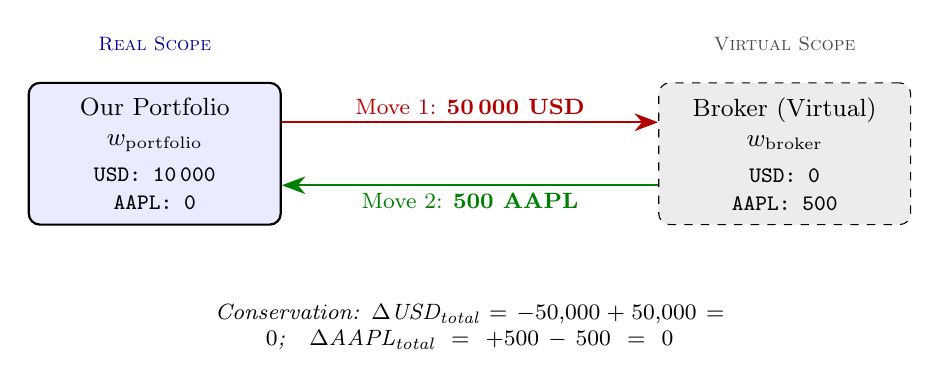
\begin{tikzpicture}[
    wallet/.style={draw, rounded corners, minimum width=3.2cm, minimum height=1.8cm, align=center, font=\small},
    real/.style={wallet, fill=blue!8, thick},
    virtual/.style={wallet, fill=gray!15, dashed},
    move/.style={-{Stealth[length=3mm]}, thick},
    label/.style={font=\footnotesize, midway, fill=white, inner sep=1.5pt},
  ]
  % Wallets
  \node[real]    (port) at (0,0)   {Our Portfolio\\$w_{\text{portfolio}}$\\[2pt]\footnotesize\texttt{USD: 10\,000}\\[-1pt]\footnotesize\texttt{AAPL: 0}};
  \node[virtual] (broker) at (8,0) {Broker (Virtual)\\$w_{\text{broker}}$\\[2pt]\footnotesize\texttt{USD: 0}\\[-1pt]\footnotesize\texttt{AAPL: 500}};

  % Moves
  \draw[move, color=red!70!black]
    ($(port.east)+(0,0.4)$) -- node[label, above=1pt] {Move 1: \textbf{50\,000 USD}} ($(broker.west)+(0,0.4)$);
  \draw[move, color=green!50!black]
    ($(broker.west)+(0,-0.4)$) -- node[label, below=1pt] {Move 2: \textbf{500 AAPL}} ($(port.east)+(0,-0.4)$);

  % Conservation annotation
  \node[font=\footnotesize\itshape, text width=7cm, align=center] at (4,-2.2)
    {Conservation: $\Delta\text{USD}_{\text{total}} = -50{,}000 + 50{,}000 = 0$;\quad $\Delta\text{AAPL}_{\text{total}} = +500 - 500 = 0$};

  % Scope labels
  \node[font=\scriptsize, color=blue!60!black] at (0,1.4) {\textsc{Real Scope}};
  \node[font=\scriptsize, color=gray!60!black] at (8,1.4) {\textsc{Virtual Scope}};
\end{tikzpicture}
\caption{Wallet-flow diagram for a share purchase: 500 AAPL shares at \$100 each. Cash moves from the real portfolio wallet to the virtual broker wallet; shares move in the opposite direction. Both moves execute atomically as a single transaction. The total quantity of each unit across all wallets is conserved.}
\label{fig:wallet-flow}
\end{figure}

\subsection{Books and Reference Wallets}

In practice, firms group trading activity into \textit{books} or \textit{accounts} for reporting and governance. Each book is associated with one or more real wallets and often with a distinguished \textit{reference wallet} holding the book's positions and cash. This grouping is a reporting convention: mathematically, all definitions and smart contracts operate at the wallet level. The managed-account smart contracts in Section~\ref{sec:managed} act on such reference wallets, regardless of whether they are classified as real or virtual.

\subsection{The Self-Consistency Principle}

The architecture is designed so that internally inconsistent states are structurally unreachable within the ledger's scope, not merely detectable after the fact.

\begin{principle}[Self-Consistency]
The ledger's conservation law, atomic transactions, and canonical event log must make internally inconsistent states structurally unreachable. Internal reconciliation---the process of comparing two independent records of the same reality within the firm---is a symptom of a multi-source-of-truth architecture. In a self-consistent system, the balance sheet IS the ledger viewed through an accounting lens; within the ledger, there is no second record to reconcile against. External systems---custodians, CSDs, counterparties, regulators---maintain independent records, and reconciliation at the ledger boundary remains necessary.
\end{principle}

This has immediate consequences for the most damaging reconciliation failures:

\begin{itemize}
\item \textbf{Trading system / general ledger divergence}: Conventionally, the front-office trading system and general ledger are separate systems connected by batch interfaces. When the interface fails, is delayed, or transmits a different version of the trade, the systems diverge. Here, the trade and its accounting entry are the same object---a transaction in the move stream. There is no second system to diverge from.

\item \textbf{PnL / balance sheet mismatch}: Conventionally, PnL is computed in one system (risk/front-office) and the balance sheet in another (general ledger), using different data sources, timing, and rounding. Here, PnL $= V_{t_1} - V_{t_0}$ is a theorem: both values derive from the same position set and price vector. There is no separate PnL system.

\item \textbf{Inter-entity breaks}: When two legal entities within the same group record different amounts for the same inter-company transaction---because each has its own ledger---the discrepancy must be reconciled. Here, the inter-entity move is a single atomic event recorded once. Within a shared ledger, disagreement is impossible.
\end{itemize}

The remaining failure modes---custodian breaks, nostro/vostro discrepancies (where ``nostro'' is our account at a correspondent bank, and ``vostro'' is a correspondent's account at our institution), counterparty disputes---are boundary conditions where the external world is an independent actor. The architecture cannot prevent an external custodian from disagreeing; it can only make disagreement detectable (via virtual wallet comparison) and narrowly scoped (via ISO 20022 feedback loops).

\noindent\textbf{Settlement timing and Herstatt risk.} The framework's atomic transaction model represents the \emph{economic intent} of simultaneous settlement. In practice, FX and cross-border transactions settle asynchronously: currency legs settle in different time zones, and CLS (Continuous Linked Settlement) provides payment-versus-payment within a specific window but not instantaneous atomicity. The framework models this by recording the trade as an atomic transaction at trade time (capturing economic intent) and tracking settlement status per leg via unit state or move metadata. Between trade and settlement, the framework represents the settlement risk as an unsettled receivable (a position in the virtual wallet of the settling counterparty). This is a modelling convention, not a risk elimination: Herstatt risk is a real-world timing risk that no ledger design can eliminate, only represent and monitor.

\clearpage
%==============================================================================
\section{The Unit Store}
\label{sec:unit-store}
%==============================================================================

Section~\ref{sec:ledger} defined the unit universe $\mathcal{U}$ and the balance function $w_t : \mathcal{U} \to \mathbb{R}$, but left $\mathcal{U}$ abstract. This section makes it concrete. The \textbf{Unit Store} is the component that manages $\mathcal{U}$: it decides what units exist, records their properties, binds each unit to a smart contract, and enforces validity at registration time. Every downstream component---the executor, the settlement projection, the valuation function---depends on the Unit Store for a well-defined, validated unit universe.

\subsection{What Is a Unit?}

A unit is any financial instrument that can appear as a balance in a wallet. The universe of units spans:

\begin{itemize}[nosep]
\item \textbf{Cash}: currencies (USD, EUR, JPY, \ldots)---dozens of entries.
\item \textbf{Listed equities}: securities identified by ISIN---tens of thousands across global exchanges.
\item \textbf{Listed derivatives}: option series and futures contracts defined by exchange contract specifications---millions of active series.
\item \textbf{OTC derivatives}: each bilateral trade is a distinct unit because counterparty identity and collateral terms (CSA) affect economics---unbounded.
\item \textbf{Bonds}: government and corporate debt identified by ISIN---millions.
\item \textbf{Structured products}: issuer warrants, securitised notes, each issuance with bespoke terms.
\end{itemize}

\noindent Units are not a flat set. Each unit has \emph{identity} (how it is uniquely distinguished from all other units), \emph{type} (what kind of instrument it is), \emph{terms} (its static contractual parameters), a \emph{smart contract} (the lifecycle logic that governs it), and a \emph{lifecycle stage} (its current state).

\subsection{Unit Identity: The OTC vs.\ Listed Distinction}
\label{sec:unit-identity}

The central design question is: \emph{when are two positions in the ``same'' instrument actually positions in the same unit?} The answer depends on fungibility.

\begin{principle}[Unit Identity]
Two positions are in the same unit if and only if they are fungible: a holder is economically indifferent between them. Positions that are fungible share a single unit entry and net against each other. Positions that are not fungible are distinct units with distinct entries.
\end{principle}

This principle produces different identity rules for different instrument classes:

\begin{center}
\small
\begin{tabular}{l l l}
\toprule
\textbf{Instrument class} & \textbf{Unit identity derived from} & \textbf{Fungibility} \\
\midrule
Cash (USD, EUR) & Currency code & All USD balances are fungible \\
Listed equity & ISIN & All shares of same ISIN net \\
Listed derivative & Contract specification & All positions in same series net \\
 & (exchange, underlier, type, strike, expiry) & (via CCP novation) \\
OTC derivative & Full CDM Trade object & Non-fungible: counterparty \\
 & (includes counterparty + Collateral) & and CSA make each trade unique \\
Bond & ISIN & All holdings of same ISIN net \\
Structured note & ISIN + product terms & Same issuance is fungible \\
Tokenized equity & Contract address + chain ID & All tokens on same contract net \\
 & (+ underlying ISIN) & (underlying tracked separately) \\
\bottomrule
\end{tabular}
\end{center}

\noindent Tokenized securities introduce a new identity pattern: the token is a distinct unit from the underlying security (see Section~\ref{sec:cdm-tokenized}). NVDA and tokenized-NVDA are different units with different settlement mechanisms, even though they carry the same economic exposure. The custodian holding the underlying shares nets to zero economic exposure (long NVDA, short NVDA\_TOKEN); the double-counting resolution is developed in Section~\ref{sec:cdm-tokenized}.

\medskip
\noindent The key insight, developed in Appendix~\ref{app:cdm-walkthrough}: for OTC instruments, the unit identity is the CDM \texttt{Trade} object including its \texttt{Collateral} field. Two OTC trades with identical payoff terms but different CSAs (e.g., USD CSA vs.\ EUR CSA) are \textbf{different units}---they have different discount curves, different margin flows, and different settlement currencies. For listed instruments, the CCP interposes itself as the sole counterparty via novation, making all positions in the same contract specification fungible regardless of the original counterparty.

\subsection{Three-Tier Architecture}

The Unit Store is organised in three tiers, each serving a distinct purpose.

\subsubsection{Tier 1: Reference Data}

\textbf{Source}: exchanges, reference data vendors, CSD records.\\
\textbf{Content}: instrument master data---ISIN, exchange, contract specification (underlier, strike, expiry, multiplier, settlement currency), issuer, coupon schedule.\\
\textbf{CDM mapping}: \texttt{TransferableProduct} for securities (equities, plain bonds); \texttt{NonTransferableProduct} for derivatives and structured products.\\
\textbf{Lifecycle}: read from external sources. The Ledger does not create reference data; it consumes it.

This tier answers: \emph{what instruments exist in the market?}

\subsubsection{Tier 2: Product Registry}

\textbf{Source}: CDM product qualification applied to Tier~1 data and OTC trade terms.\\
\textbf{Content}: the smart contract template that governs each product type. One entry per product type, not per individual contract---e.g., ``European equity index option'' maps to an \texttt{OptionPayout} contract template that handles all European equity index options regardless of underlier, strike, or expiry.\\
\textbf{CDM mapping}: CDM \texttt{ProductQualification} functions classify \texttt{EconomicTerms} into product types; each product type maps to a Ledger smart contract template (Section~\ref{sec:contracts}).\\
\textbf{Lifecycle}: entries are created automatically when a Tier~3 registration encounters a product type not yet in the registry. Once created, entries are immutable.

This tier answers: \emph{what lifecycle logic governs this kind of instrument?}

\subsubsection{Tier 3: Unit Registry}

\textbf{Source}: trade events (execution reports, reference data feeds, lifecycle events).\\
\textbf{Content}: the actual units that appear as wallet balances---the elements of $\mathcal{U}$.\\
\textbf{CDM mapping}: for listed instruments, the unit corresponds to the contract specification (a \texttt{NonTransferableProduct} or \texttt{TransferableProduct}); for OTC instruments, the unit corresponds to the full CDM \texttt{Trade} (including \texttt{Collateral}).

Each unit entry in the registry contains:

\begin{lstlisting}
UnitEntry:
    unit_id          : UniqueId          -- deterministic, from CDM object
    unit_type        : UnitType          -- CASH | EQUITY | LISTED_DERIV
                                         --   | OTC_DERIV | BOND | STRUCTURED
    -- Identity (varies by type)
    isin             : Option<ISIN>      -- securities, bonds, structured notes
    contract_spec    : Option<ContractSpec>  -- listed derivatives
    cdm_trade_ref    : Option<TradeRef>  -- OTC (includes Collateral)

    -- Product binding
    product_ref      : ProductRegistryRef  -- pointer to Tier 2 entry
    smart_contract   : SmartContractRef    -- lifecycle logic instance

    -- Terms (from CDM EconomicTerms)
    currency         : CurrencyCode
    multiplier       : Option<Decimal>
    expiry           : Option<Date>

    -- Lifecycle
    lifecycle_stage  : PENDING | ACTIVE | MATURED | TERMINATED | SETTLED
    unit_state       : ProductSpecificState  -- see Section 7 (Lifecycle)

    -- Provenance
    created_by       : TransactionId     -- registering transaction
    created_at       : Timestamp
\end{lstlisting}

\noindent The \texttt{lifecycle\_stage} is the coarse-grained lifecycle position (common to all unit types). The \texttt{unit\_state} is the product-specific state dictionary defined in Section~\ref{sec:lifecycle}---e.g., which coupons have been paid for a bond, or the accumulated cost for a futures position. The Unit Store owns the entry; the lifecycle engine (Section~\ref{sec:lifecycle}) drives state transitions.

The \texttt{unit\_id} is derived deterministically from the CDM object: for listed instruments, it is a hash of the contract specification fields; for OTC instruments, it is the CDM Trade's identifier (UTI or metadata key). The derivation is injective: distinct CDM objects always produce distinct unit IDs (as required by Appendix~\ref{app:cdm-walkthrough}, Section~\ref{sec:cdm-implications}).

This tier answers: \emph{what specific units can appear in wallet balances right now?}

\subsection{How Units Enter the Store}
\label{sec:unit-registration}

Units enter the registry through three channels, each corresponding to an instrument class:

\begin{enumerate}
\item \textbf{Cash (pre-registered).} Currency units (USD, EUR, GBP, JPY, etc.) are permanent entries created at system initialisation. They have no expiry, no lifecycle events, and lifecycle stage \texttt{ACTIVE} permanently. Their smart contract is the identity function (cash moves require no lifecycle logic). Registration is an administrative operation at system inception.

\item \textbf{Listed instruments (reference data feed).} When a new exchange product is listed or when the Ledger is initialised against an existing market, the reference data feed provides the contract specification. The Unit Store creates a Tier~1 entry (reference data), a Tier~2 entry (product registry, if the product type is new), and a Tier~3 entry (unit registry). This is an administrative operation, not a trade. The unit exists before any position is taken; it enters $\mathcal{U}$ upon listing, not upon first trade.

\item \textbf{OTC instruments (trade execution).} When an OTC trade is executed, the CDM \texttt{Trade} object \emph{is} the unit definition. The Unit Store creates a Tier~3 entry from the Trade. The unit ID is derived from the Trade's metadata key---which includes counterparty and \texttt{Collateral}, ensuring that two trades with identical payoffs but different CSAs receive different unit IDs. The unit enters $\mathcal{U}$ at trade execution and is specific to that bilateral agreement.
\end{enumerate}

\noindent In all cases, registration is atomic: either the unit is fully validated and added, or it is rejected with no partial state change. Units are never deleted from the store; when a unit reaches end of lifecycle (maturity, termination, full settlement), its \texttt{lifecycle\_stage} transitions to \texttt{MATURED}, \texttt{TERMINATED}, or \texttt{SETTLED}. The entry remains for audit, time travel, and historical queries, but the executor rejects new moves against non-\texttt{ACTIVE} units (except for settlement of existing obligations).

\subsection{Correctness Enforcement}
\label{sec:unit-validation}

The Unit Store enforces validity at two points: registration time and transaction time.

\medskip
\noindent\textbf{At registration}, a unit must satisfy:
\begin{enumerate}[nosep]
\item \textbf{Uniqueness}: no existing unit has the same \texttt{unit\_id}.
\item \textbf{Smart contract binding}: a smart contract reference exists for the unit's product type.
\item \textbf{CDM qualification}: for CDM-native units, the CDM \texttt{ProductQualification} function returns a valid classification for the stated \texttt{EconomicTerms}. An unclassifiable product is rejected.
\item \textbf{Term consistency}: static terms are internally consistent (e.g., expiry is in the future at creation, multiplier is positive, currency code is valid).
\end{enumerate}

\noindent\textbf{At transaction time}, the executor validates that every unit referenced in a move:
\begin{enumerate}[nosep]
\item exists in the Unit Store,
\item has lifecycle stage \texttt{ACTIVE} (or a stage compatible with the requested operation), and
\item has a smart contract that the executor can invoke for the requested event.
\end{enumerate}

\noindent This two-stage validation ensures that invalid units cannot enter $\mathcal{U}$ and that moves cannot reference non-existent or retired units. Combined with the conservation law (Section~\ref{sec:ledger}) and the executor's purity requirements (Section~\ref{sec:lifecycle}), the Unit Store completes the chain of correctness: the ledger operates only on well-defined, validated, contract-governed units.

\subsection{Guarantees}

The Unit Store provides four guarantees to all downstream consumers:

\begin{enumerate}
\item \textbf{Existence}: every unit referenced in a move exists in the registry and is in a valid lifecycle stage.
\item \textbf{Immutability}: a unit's identity and static terms are fixed at registration. The same \texttt{unit\_id} always refers to the same instrument with the same contractual parameters. (Lifecycle stage and unit state evolve; identity and terms do not.)
\item \textbf{Smart contract availability}: every registered unit has a bound smart contract that the executor can invoke for lifecycle events.
\item \textbf{CDM alignment}: every CDM-native unit maps to a CDM object (\texttt{Trade}, \texttt{NonTransferableProduct}, or \texttt{TransferableProduct}) with a successful product qualification.
\end{enumerate}

\noindent These guarantees make the referential integrity invariant (P3 in Section~\ref{sec:invariants}) enforceable by construction: $m.\text{unit} \in \mathcal{U}$ holds because the executor checks the Unit Store before accepting any move.

\subsection{CDM Alignment}

Each tier of the Unit Store maps to a CDM concept:

\begin{center}
\small
\begin{tabular}{l l l}
\toprule
\textbf{Tier} & \textbf{Content} & \textbf{CDM equivalent} \\
\midrule
1 (Reference Data) & Instrument master data & \texttt{TransferableProduct} (securities), \\
 & & \texttt{NonTransferableProduct} (derivatives) \\
2 (Product Registry) & Smart contract templates & \texttt{ProductQualification} + \texttt{EconomicTerms} \\
3 (Unit Registry) & Position-bearing units ($\mathcal{U}$) & \texttt{Trade} (OTC), contract spec (listed) \\
\bottomrule
\end{tabular}
\end{center}

\noindent\textbf{CDM gaps.} CDM does not have a native ``unit store'' concept---it models individual trades, not catalogues. CDM's listed derivative coverage is thinner than its OTC coverage: the same \texttt{NonTransferableProduct} type serves both, without a dedicated ``contract specification'' type for exchange listings. CDM does not model exchange reference data feeds (contract listings, expiry calendars, lot sizes). These are documentation gaps, not design incompatibilities: the Unit Store uses CDM objects as its internal representation; catalogue management is a Ledger-specific concern that sits alongside CDM, not against it.

\clearpage
%==============================================================================
\section{Portfolio Valuation and PnL}
\label{sec:valuation}
%==============================================================================

The valuation framework follows directly from the wallet structure. Because ownership is encoded as wallet balances, and because conservation ensures quantities are always consistent, valuation reduces to: multiply each position by its price and sum.

\medskip
\noindent\textbf{Quantity conservation vs.\ value conservation.} The conservation law (Section~\ref{sec:ledger}) guarantees \emph{quantity} balance: the total quantity of each unit across all wallets is zero. This is an algebraic invariant proved from the move semantics. \emph{Value} conservation---the invariance of total portfolio value $V_t = \sum w_t(u) \cdot P_t(u)$---does not follow from the conservation law alone, because prices are external inputs that change independently of ledger activity. An FX trade conserves EUR quantities and USD quantities separately, but the market value of the EUR received may differ from the USD paid at any rate other than the trade rate. Value conservation holds exactly only for deterministic lifecycle events (Section~\ref{sec:intro}, Property~5). The distinction is fundamental: conservation guarantees quantity integrity; the valuation layer captures value changes due to price movements. CDM's normalised quantity and price representations ensure standard-form inputs, eliminating unit-conversion ambiguities that arise when different systems use different notional conventions.

\subsection{Mark-to-Market Valuation}

\begin{definition}[Portfolio Value]
Let $P_t : \mathcal{U} \to \mathbb{R}$ be a price function at time $t$. The portfolio value represents the quantity of reference currency (typically USD) that would remain if every position were unwound at current market prices:
\[
V_t = \sum_{u \in \mathcal{U}} w_t(u) \cdot P_t(u)
\]
where the reference currency has $P_t(\text{USD}) = 1$. The price function $P_t$ is an \emph{external input} to the framework, not computed by it. For listed instruments, $P_t(u)$ is the exchange-quoted price; for OTC derivatives, it is the output of an external pricing model (Black-Scholes, Monte Carlo, etc.); for bespoke structured products, it may be a dealer quote or internal model valuation. The framework is agnostic to the pricing methodology---it requires only that $P_t$ be supplied as a function from units to prices in the reference currency. The framework requires a designated reference currency for all prices; for a multi-currency portfolio, the choice of reference currency and FX rates are additional parameters affecting reported PnL. Note that $P_t(u)$ assumes orderly markets with sufficient liquidity; in stressed conditions (market halts, exchange closures, counterparty default), the price function may be stale, unavailable, or may not reflect achievable liquidation values.
\end{definition}

\subsection{State-Sufficiency}

\begin{principle}[State-Sufficiency]
Portfolio value at time $t$ depends only on current wallet balances, current unit state (including all embedded lifecycle state such as accrued interest, exercise flags, and barrier status), and current prices---provided all economically relevant state changes have been recorded in the unit state. Transaction history is irrelevant given this precondition.
\end{principle}

\noindent State-sufficiency has a practical consequence: computing portfolio value requires only a snapshot of wallet balances and a price vector, not a replay of transaction history. This makes PnL computation $O(n)$ in instruments rather than $O(m)$ in moves.

\subsection{Path-Independent PnL Theorem}

\begin{theorem}[Path-Independent PnL]
The profit and loss over interval $[t_0, t_1]$ is:
\[
\text{PnL} = V_{t_1} - V_{t_0}
\]
This depends only on the portfolio states at $t_0$ and $t_1$, not on intermediate transactions.
\end{theorem}

\noindent\textit{Proof.} Both $V_{t_0}$ and $V_{t_1}$ are determined by wallet balances and prices at their respective times. Wallet balances are the cumulative effect of all moves up to that time. If intermediate snapshots are taken at times $t_0 < s_1 < s_2 < \cdots < s_k < t_1$, the telescoping sum
\[
V_{t_1} - V_{t_0} = (V_{t_1} - V_{s_k}) + (V_{s_k} - V_{s_{k-1}}) + \cdots + (V_{s_1} - V_{t_0})
\]
shows that the total PnL is the sum of incremental changes, and the intermediate values $V_{s_i}$ cancel. No information about the path of transactions between $t_0$ and $t_1$ enters the formula. \qed

\noindent The content of this result is not that a telescoping sum telescopes---that is the proof mechanism---but that total PnL is independent of trading activity between $t_0$ and $t_1$. A portfolio that executed 10{,}000 intermediate trades has the same total PnL as one that executed none, provided the final positions and prices match. This is non-trivial because it means PnL computation never requires replaying intermediate transactions---only the initial and final snapshots matter.

\noindent\textbf{Qualification.} This result holds given that all economically relevant state changes---fees, corrections, lifecycle events, corporate actions---are recorded as moves in the ledger. If a state change occurs outside the ledger (e.g., an unrecorded fee, a bilateral agreement not yet booked), the theorem does not capture it. The result is a consequence of the framework's modelling choice: the ledger records all economic activity within its scope, and PnL is defined as the change in the ledger's valuation.

\noindent\textbf{Scope note.} The PnL defined here is \textit{economic} PnL: the change in fair value of positions. Accounting PnL under IFRS~9 or US~GAAP depends on instrument classification (FVTPL, FVOCI, or amortised cost), which determines whether fair-value changes flow through profit or loss, other comprehensive income, or are recognised only on derecognition. Accounting classification is outside the ledger's scope; the framework guarantees correct position quantities and economic valuations from which accounting PnL can be derived.

\subsection{PnL Decomposition with Full Numerical Example}

\begin{proposition}[PnL Attribution]\hfill
\[
\text{PnL} = \text{PnL}_{\text{price}} + \text{PnL}_{\text{flow}}
\]
where:
\[
\text{PnL}_{\text{price}} = \sum_i w_{t_0}(i) \cdot [P_{t_1}(i) - P_{t_0}(i)]
\]
\[
\text{PnL}_{\text{flow}} = \Delta w(\text{USD}) + \sum_i \Delta w(i) \cdot P_{t_1}(i)
\]
\end{proposition}

\noindent\textbf{Numerical Example.}

\begin{center}
\begin{tabular}{l r r r}
\toprule
\textbf{Event} & \textbf{USD} & \textbf{AAPL shares} & \textbf{AAPL Price} \\
\midrule
\textit{Initial state at $t_0$} & 1{,}000 & 10 & 100 \\
Portfolio value $V_{t_0}$ & \multicolumn{2}{l}{$= 1{,}000 + (10 \times 100) = 2{,}000$} & \\
\midrule
\textit{Transaction 1: Buy 5~shares at \$100} & & & \\
\quad Move 1: USD payment & $-500$ & $+0$ & \\
\quad Move 2: Share receipt & $+0$ & $+5$ & \\
After transaction & 500 & 15 & 100 \\
\midrule
\textit{Transaction 2: Dividend received} & & & \\
\quad Move: Cash dividend & $+20$ & $+0$ & \\
After transaction & 520 & 15 & 100 \\
\midrule
\textit{Transaction 3: Trading fees paid} & & & \\
\quad Move: Fee payment & $-5$ & $+0$ & \\
After transaction & 515 & 15 & 100 \\
\midrule
\textit{Transaction 4: Financing cost} & & & \\
\quad Move: Interest charge & $-8$ & $+0$ & \\
After transaction & 507 & 15 & 100 \\
\midrule
\textit{Price change to $t_1$} & 507 & 15 & 110 \\
Portfolio value $V_{t_1}$ & \multicolumn{2}{l}{$= 507 + (15 \times 110) = 2{,}157$} & \\
\bottomrule
\end{tabular}
\end{center}

\noindent\textbf{PnL Analysis:}
\begin{align*}
\text{Total PnL} &= V_{t_1} - V_{t_0} = 2{,}157 - 2{,}000 = 157 \\
\text{PnL}_{\text{price}} &= 10 \times (110 - 100) = 100 \quad \text{(price appreciation on initial holding)} \\
\text{PnL}_{\text{flow}} &= (507 - 1{,}000) + 5 \times 110 = -493 + 550 = 57 \\
&\quad\text{(cash flow impact: $-500$ purchase, $+20$ dividend, $-5$ fees, $-8$ financing)} \\
\text{Verification:} &\quad 100 + 57 = 157 \checkmark
\end{align*}

All cash flows (purchases, dividends, fees, financing) appear as explicit wallet moves affecting the USD balance, while price changes affect only the valuation of existing positions.

\clearpage
%==============================================================================
\section{Smart Contracts as Move Generators}
\label{sec:contracts}
%==============================================================================

The closed ledger framework treats financial instruments as deterministic programs that emit moves, not as opaque objects stored in a database. A bond emits coupon payments and a final redemption. An option emits a premium at inception and a conditional payoff at expiry. A swap emits periodic net payments. The program logic can be complex, but its output is always the same: a list of moves.

\subsection{Contract Definition}

\begin{definition}[Smart Contract]
A smart contract is a deterministic program that maps inputs and state to sequences of atomic moves:
\[
\textit{Contract} : (\textit{Input}, \textit{State}, \textit{Conditions}) \to \{\textit{Moves}\}
\]
\end{definition}

\noindent Given the same inputs, state, and market conditions, a contract always produces the same moves. There is no randomness, no hidden state, no external dependency beyond the explicitly passed parameters. Determinism requires that arithmetic be reproducible across platforms: an implementation must use fixed-precision decimal arithmetic (not IEEE~754 floating-point, which is not associative) for all balance and payment calculations. Bankers' rounding (IEEE~754 ``round half to even'') is applied at instruction generation---the point where an exact internal amount is projected to a settlement or payment message. Quantities and prices are represented as exact decimals with a defined precision (e.g., 18 decimal places). This ensures that the same inputs produce bit-identical outputs regardless of hardware or compiler, which is a precondition for reproducible time travel and cross-system verification.

The contract is not stored separately from the ledger---its effects ARE ledger entries. Product complexity is isolated in the contract; the ledger sees only moves.

Adding a new product type requires only defining a new contract (a deterministic function from inputs and state to moves). No changes to the ledger engine, move stream, balance computation, or reporting infrastructure are needed. The new product's moves are indistinguishable from existing products' moves at the ledger level.

A smart contract in this framework is the machine-readable, executable form of the legal confirmation. An ISDA derivatives confirmation already describes the product, economics, lifecycle events, and settlement obligations in structured terms. CDM is the formal vocabulary of that structure---how ISDA documentation is expressed as data. Writing the smart contract from the confirmation is therefore a transcription, not an engineering exercise, because the vocabulary is shared. CDM enums map directly to product types, lifecycle events, and settlement obligations in the confirmation. The smart contract adds executability; it adds nothing to the information content.

\subsection{Smart Contract Composition: Modular vs Composite}

A natural question arises: should each payout type have its own smart contract (one script for the option payoff, a separate script for the CSA margin), or should there be one composite smart contract per instrument type (a single script for a call-with-CSA)?

The framework recommends the modular approach: one smart contract per payout or obligation type. The reasons are:

First, separation of concerns. The option payoff depends on the strike, the spot, and the exercise terms. The CSA margin depends on the aggregate mark-to-market, the threshold, the minimum transfer amount (MTA), and the eligible collateral currency. These are independent calculations with independent inputs. Combining them into a single script creates coupling without benefit.

Second, reusability. The CSA margin contract is the same regardless of whether the underlying trade is an option, a swap, or a structured note. Writing it once and attaching it to any collateral wallet eliminates duplication and reduces the surface area for bugs.

Third, testability. A pure function that computes option exercise moves can be tested in isolation with synthetic inputs. A pure function that computes margin calls can be tested in isolation. A composite function that does both is harder to test because its input space is the product of both---and most of that product space is irrelevant (the option payoff does not depend on the MTA, and the margin call does not depend on the strike).

The trade-off: the modular approach requires clear interfaces between contracts. The executor---the single component permitted to mutate the ledger, defined formally in Section~\ref{sec:lifecycle}---must orchestrate the correct sequence of contract invocations for a given lifecycle event. This orchestration is itself a design concern---but it is a simpler concern than the alternative of maintaining composite scripts for every product-CSA combination.

\subsection{Equity Contracts}

A stock contract emits moves for three event types: trade execution, dividend payments, and corporate actions. All three use the same primitive---a set of moves in a transaction---with no separate machinery for dividends or splits.

\noindent\textbf{Trade execution.} A purchase of $n$ shares at price $p$ is a transaction containing two moves: $n \times p$ units of cash from buyer wallet to seller wallet, and $n$ units of the stock from seller wallet to buyer wallet. Both moves execute atomically.

\noindent\textbf{Dividend payment.} On the ex-dividend date, the contract emits a cash move from an issuer virtual wallet to each holder wallet, proportional to shares held. The unit state records the dividend event (date and amount per share) to ensure idempotency.

\noindent\textbf{Bond trades and accrued interest.} When a bond trades between coupon dates, the buyer pays the dirty price (clean price plus accrued interest). In the framework, accrued interest is not a separate unit; instead, the bond's price function $P_t(u)$ returns the \emph{dirty} price (which includes accrual), and the trade is recorded as a cash-for-bond exchange at the dirty price. On the next coupon date, the lifecycle event pays the full coupon and transitions the bond ex-coupon. The clean/dirty distinction is a reporting convention derived from the bond's unit state (which records the last coupon date and accrual convention), not a separate position. For valuation, the system can report both clean and dirty prices by subtracting accrued interest computed from the unit state.

\noindent\textbf{Corporate actions.} Corporate actions such as stock splits span multiple dates: announcement date, record date (determining entitled holders), ex-date (when the market price adjusts), and payment/effective date. In the framework, a corporate action is modelled as a sequence of state transitions and moves anchored to these dates. At the record date, the unit state records the entitlement snapshot (which wallets hold positions). At the ex-date or effective date, the contract emits the position-adjustment moves: for a 2-for-1 split, this doubles the share count in each entitled wallet via moves from a corporate-action virtual wallet, while the price reference adjusts. The ledger records each step as a transaction with full metadata (dates, ratios, entitlement rules), enabling time travel to reconstruct both pre-action and post-action views. The same multi-date mechanism handles mergers, spin-offs, and rights issues, where each date (announcement, record, effective, payment) triggers a distinct lifecycle event.

\subsection{European Put Option---Full Move Schedule}

\noindent\textbf{Contract Specification:}
\begin{itemize}[nosep]
\item Strike price: $K$
\item Expiry date: $T$
\item Underlying asset: $S$
\item Notional quantity: $N$
\item Counterparties: buyer wallet $w_B$, seller wallet $w_S$
\item Premium: $P$
\end{itemize}

\noindent\textbf{Move Schedule.}
The contract is completely defined by conditional moves at inception and expiry.

\noindent\textit{Move 1 (at inception, $t = 0$):}

\begin{lstlisting}
Move(
    from: w_B,
    to: w_S,
    unit: USD,
    quantity: P * N,
    timestamp: t_0,
    source: "put_contract_ref_id",
    metadata: "PUT_PREMIUM"
)
\end{lstlisting}

This move is unconditional and executes immediately upon contract creation.

\noindent\textbf{Case 1: Cash Settlement.}\\
\textit{Move 2 (at expiry, $t = T$):}\\
If $S_T < K$ (put is in-the-money):

\begin{lstlisting}
Move(
    from: w_S,
    to: w_B,
    unit: USD,
    quantity: (K - S_T) * N,
    timestamp: T,
    source: "put_contract_ref_id",
    metadata: "PUT_SETTLEMENT_CASH"
)
\end{lstlisting}

If $S_T \geq K$ (put is out-of-the-money): no move executes.

In cash settlement, only a net cash payment is exchanged. If the put is in-the-money ($S_T < K$), the seller pays the buyer the intrinsic value $(K - S_T) \cdot N$ in USD.

\noindent\textbf{Case 2: Physical Delivery.}\\
\textit{Moves 2a and 2b (at expiry, $t = T$):}\\
If $S_T < K$ (put is in-the-money):

\begin{lstlisting}
Move(
    from: w_B,
    to: w_S,
    unit: S,                    -- ISIN code of underlying asset
    quantity: N,
    timestamp: T,
    source: "put_contract_ref_id",
    metadata: "PUT_DELIVERY_ASSET"
)

Move(
    from: w_S,
    to: w_B,
    unit: USD,
    quantity: K * N,
    timestamp: T,
    source: "put_contract_ref_id",
    metadata: "PUT_DELIVERY_CASH"
)
\end{lstlisting}

If $S_T \geq K$: no moves execute. In physical delivery, the buyer delivers $N$ units of the underlying asset to the seller and receives the strike price $K \cdot N$ in cash. The two moves execute atomically as a single transaction, ensuring simultaneous exchange of asset and cash. This requires the buyer to hold the underlying asset in their wallet at expiry.

\noindent\textbf{Physical Delivery with Lot-Size Constraints.}
Equity delivery requires whole multiples of the board lot (a property of the underlying, recorded in the Unit Store's reference data). When $N$ is not an exact multiple of the lot size~$L$, the contract computes:
\[
N_{\text{deliver}} = \left\lfloor \frac{N}{L} \right\rfloor \cdot L, \qquad N_{\text{residual}} = N - N_{\text{deliver}}.
\]
The physically delivered portion settles as a DvP pair (shares against cash at strike); the residual settles in cash at the put's intrinsic value $(K - S_T) \cdot N_{\text{residual}}$. The contract emits all moves in a single atomic transaction:

\begin{lstlisting}
Transaction(type = SETTLEMENT):
    -- Physical delivery of whole lots
    Move(from: w_B, to: w_S, unit: S, quantity: N_deliver)
    Move(from: w_S, to: w_B, unit: USD, quantity: K * N_deliver)
    -- Cash settlement of residual (put intrinsic value)
    Move(from: w_S, to: w_B, unit: USD, quantity: (K - S_T) * N_residual)
\end{lstlisting}

\noindent Conservation holds: the underlying unit nets to zero ($-N_{\text{deliver}} + N_{\text{deliver}} = 0$), and cash nets to zero (the seller's total outflow $K \cdot N_{\text{deliver}} + (K - S_T) \cdot N_{\text{residual}}$ equals the buyer's total inflow). The total economic value transferred equals the put payoff $(K - S_T) \cdot N$ regardless of the lot split---the lot-size constraint changes the delivery structure but not the economic value. The lot-size logic is a pure function of $(K, N, S_T, L)$, making it trivially testable with property-based tests (Appendix~\ref{app:properties}). The settlement projection (Section~\ref{sec:settlement}) produces two instructions from this single transaction: a securities delivery (\texttt{sese.023}) for $N_{\text{deliver}}$ shares, and a cash payment for the combined amount $K \cdot N_{\text{deliver}} + (K - S_T) \cdot N_{\text{residual}}$.

This pattern generalises to any physically settled instrument with lot constraints---convertible bond conversion, warrant exercise, equity forward delivery---because the lot-adjustment function is the same; only the payoff formula differs.

\medskip

\noindent In both cases, the contract is fully defined by its move schedule: a finite list of conditional transfers parameterised by market observables. Derivative pricing complexity (Black-Scholes, Monte Carlo, finite differences) is irrelevant to the ledger; the ledger sees only the moves the contract emits when conditions are met.

\subsection{Interest Rate Swap---Full Move Schedule}

\noindent\textbf{Contract Specification:}
\begin{itemize}[nosep]
\item Notional principal: $N$
\item Fixed rate: $r_{\text{fixed}}$
\item Floating rate reference: risk-free reference rate, e.g., the Secured Overnight Financing Rate (SOFR) (denoted $r_{\text{float},k}$ at reset $k$)
\item Reset dates: $\{t_1, t_2, \ldots, t_n\}$
\item Day count fraction: $\delta_k$ for period $k$ (e.g., ACT/360; see Section~\ref{sec:cdm-dates} for the CDM date types and day count conventions that determine the reset dates and year fractions $\delta_k$)
\item Counterparties: fixed-rate payer $w_F$, floating-rate payer $w_L$
\end{itemize}

\noindent\textbf{Move Schedule.}
For each reset $t_k$ where $k = 1, 2, \ldots, n$:

\[
\text{Payment}_k = N \cdot (r_{\text{float},k} - r_{\text{fixed}}) \cdot \delta_k
\]

\begin{lstlisting}
Move(
    from: w_F,
    to: w_L,
    unit: USD,
    quantity: Payment_k,
    timestamp: t_k,
    source: "irs_contract_ref_id",
    metadata: "IRS_NET_PAYMENT"
)
\end{lstlisting}

$\text{Payment}_k$ can be positive or negative. Because move quantities must be positive (Definition~2.3), the contract emits a move with $|\text{Payment}_k|$ as the quantity: when $\text{Payment}_k > 0$, the move goes from $w_F$ to $w_L$; when $\text{Payment}_k < 0$, the move goes from $w_L$ to $w_F$. The direction is determined by the sign; the quantity is always the absolute value. At each reset date, the contract needs only the current floating rate and the fixed parameters---no historical path is needed.

The complete contract is the sequence of settlement moves: $\text{SwapContract} = \{m_1, m_2, \ldots, m_n\}$, one per reset date. The swap's entire economic content is captured by these moves plus the unit state (which records processed resets for idempotency).

\medskip

\noindent\textbf{Worked Example: IRS Lifecycle in CDM Terms.}
Consider a 5-year USD IRS, notional \$10M, fixed rate 3\%, quarterly resets.

\noindent\textit{Step 1 --- Inception} (CDM \texttt{ExecutionEvent}, intent: \texttt{OPEN}). Unit state initialised: fixed rate, floating index, schedule, reset counter = 0. No cash moves at inception (no upfront premium for a par swap).

\noindent\textit{Step 2 --- Rate reset at $t_1$} (CDM \texttt{ResetEvent}). The floating rate is observed (e.g., SOFR = 3.5\%). Unit state updated: \texttt{float\_rate\_$t_1$} = 3.5\%, reset counter incremented.

\noindent\textit{Step 3 --- Coupon exchange at $t_1$} (CDM \texttt{TransferEvent}). Net payment computed: $10\text{M} \times (3.5\% - 3\%) \times 0.25 = 12{,}500$. Move: \texttt{Move(from: w\_F, to: w\_L, unit: USD, quantity: 12,500)}. Unit state updated: period $t_1$ marked as settled.

\noindent\textit{Step 4 --- Maturity at $t_n$} (CDM \texttt{TerminationEvent}, intent: \texttt{TERMINATE}). Final coupon exchange processed as in Step~3. Unit state transitions to TERMINATED. No further resets or payments are possible.

\clearpage
%==============================================================================
\section{Managed Accounts, Virtual Portfolios, and TRS}
\label{sec:managed}
%==============================================================================

Every wallet is a managed account. This is a structural identity, not a metaphor: a wallet holds positions, those positions generate PnL, and that PnL is periodically settled in cash. Whether the wallet belongs to a trading desk, a prime brokerage client, or a QIS investor, the mechanism is identical. This section consolidates the managed account architecture, including virtual ledgers and total return swaps.

\subsection{Wallets as Managed Accounts}

Any trading book---whether managed by internal traders, prime portfolio swap books, or QIS books---can be viewed uniformly as a managed account. Trades may be initiated by an internal trader, a hedge fund manager, or a systematic strategy, but the workflow is always identical: each trade is captured as a transaction (a finite collection of atomic moves) and fed into a designated book---a partition of real wallet balances used for position and PnL attribution.

\subsection{Reference Wallet, Performance, and the Managed-Account Smart Contract}

In ISDA terminology, it is natural to view such a book's wallet as representing a \textit{Reference Portfolio} and the party economically entitled to its performance---Treasury for internal risk-taking, or a client in a Prime Portfolio swap---as the \textit{Ultimate Beneficiary}, analogous to the Total Return Receiver in a total return swap.

Let $w_{\text{ref}} \in \mathcal{W}$ be the reference wallet for a given book. Its value under price vector $P_t$ is:
\[
V_t^{\text{ref}} = \sum_{u \in \mathcal{U}} w_{\text{ref},t}(u) \cdot P_t(u).
\]
Over each reset interval $[t_{k-1}, t_k]$, the \textit{Reference Wallet Performance Amount} is:
\[
\text{Perf}^{\text{ref}}_{[t_{k-1}, t_k]} = V^{\text{ref}}_{t_k} - V^{\text{ref}}_{t_{k-1}}.
\]

A managed-account smart contract for $w_{\text{ref}}$ is a deterministic program that, at each reset time $t_k$, performs three steps:

\begin{enumerate}
\item \textbf{Observation.} Read the state of $w_{\text{ref}}$ at $t_{k-1}$ and $t_k$ and the relevant price vectors to compute the Reference Wallet Performance Amount $\text{Perf}^{\text{ref}}_{[t_{k-1}, t_k]}$.

\item \textbf{Crystallisation.} Emit a single net cash move in the reference currency between the cash wallet associated with $w_{\text{ref}}$, denoted $w^{\text{cash}}_{\text{ref}}$, and a cash wallet representing the Ultimate Beneficiary, $w^{\text{cash}}_{\text{UB}}$:

\begin{lstlisting}
Move(
    from: w_ref_cash,
    to: w_ultimate_beneficiary_cash,
    unit: USD,
    quantity: Perf_ref_k,
    timestamp: t_k,
    source: "managed_account_contract_ref",
    metadata: "REFERENCE_PERFORMANCE_RESET"
)
\end{lstlisting}

\item \textbf{Reset.} The PnL baseline resets to the state at $t_k$; the next interval's performance is measured relative to $V^{\text{ref}}_{t_k}$.
\end{enumerate}

This three-step structure (Observe, Crystallise, Reset) applies uniformly to internal desks settled against Treasury, prime brokerage clients, and QIS investors. The only parameters that vary are the identity of the Ultimate Beneficiary, the reset frequency, and the valuation basis.

\subsection{Segregation as Algebraic Constraint}

Conservation means that \emph{logical} client asset segregation is enforced by algebra, not by operational controls. Every move has an explicit source and destination wallet; total quantity across all wallets is conserved; therefore moves within one client's wallet partition cannot affect another's balances. This provides the logical separation component of CASS Rule~6 (segregation of client assets from firm assets) and MiFID~II Article~16(8) (adequate safeguarding arrangements) through the structure of the move primitive itself. However, CASS~6 also requires \emph{legal} segregation: client assets must be held in legally distinct accounts at custodians, with appropriate trust or nominee arrangements. Legal segregation depends on custodial agreements and regulatory filings that are outside the ledger's scope. The framework enforces logical segregation by construction and provides the position data needed to evidence legal segregation, but cannot itself establish the legal separation that regulations require.

\subsection{CSA Margin as a Wallet-Level Smart Contract}

The CSA margin contract is a wallet-level smart contract. It is attached to the collateral wallet that manages margin for a bilateral relationship. It reads the aggregate mark-to-market (MTM) of all trades governed by that CSA, computes the required collateral, and generates margin call moves. Individual trades reference the CSA through their CDM \texttt{CollateralProvisions}, but the margin calculation operates at the portfolio level---this is how bilateral CSAs work in practice, and the framework models it directly.

The CSA governs a bilateral relationship between two parties across potentially many trades. In practice, a single CSA covers an entire portfolio of trades between a firm and a counterparty. The collateral wallet (where margin is posted and received) is per-counterparty, not per-trade. The CSA smart contract reads the aggregate MTM across all trades under that CSA, computes the required margin (applying thresholds, minimum transfer amounts, and eligible collateral rules), and generates moves to or from the collateral wallet. This is consistent with CDM: \texttt{CollateralProvisions} attaches at the Trade level to indicate \emph{which} CSA governs, but the CSA itself operates at the portfolio (wallet) level. The liveness guarantee for CSA margin delivery---ensuring that a margin call is either discharged by the counterparty or triggers close-out netting compensation---is formalised as the obligation workflow in Section~\ref{sec:obligation-liveness}, with a worked example in Section~\ref{sec:obligation-example-csa}.

\subsection{Mandate Constraints as Smart Contract Guards}

Investment mandates include both \emph{quantitative} constraints (asset class limits, concentration limits, leverage caps, currency restrictions) and \emph{qualitative} constraints (best execution, investment suitability, prudent person standards). Quantitative constraints are expressed as preconditions on the smart contract's move-generation function. Before emitting moves, the contract evaluates these constraints against the current wallet state. If a proposed trade would violate a quantitative constraint, the contract rejects it: no moves are emitted, and the wallet state is unchanged. For quantitative constraints, mandate enforcement is deterministic and auditable: the same wallet state and proposed trade always produce the same accept/reject decision. In CDM terms, quantitative mandate constraints are validation rules evaluated before a \texttt{BusinessEvent} is admitted to the ledger.

Qualitative constraints---best execution, suitability, prudent person---require judgment and cannot be fully expressed as smart contract preconditions. The framework can enforce necessary conditions (e.g., ``trade must be within the permitted instrument universe'') but not sufficient conditions for qualitative compliance. Qualitative mandate compliance requires external governance processes; the ledger provides the data (execution prices, timing, alternatives considered) needed to evidence compliance, but does not automate the judgment itself.

\subsection{Virtual Ledgers}
\label{sec:virtual-ledger}

A \textit{virtual ledger} is a separate instance of the same ledger framework in which every wallet is virtual, holding no real assets and connected to no custody or settlement system. It uses the same wallet, move, conservation, and lifecycle machinery as the real ledger---a second instantiation, not a separate system. Its purpose is pure strategy simulation: performance monitoring, ``what-if'' analysis, and performance attribution, with full time-travel and lifecycle capabilities. No real cash flows occur; all positions and flows are simulated.

\begin{definition}[Virtual Ledger]
A virtual ledger $\mathcal{L}_v$ is a complete ledger instance---wallets, move stream, unit state, conservation law, lifecycle engine---in which every wallet is virtual. It is closed and self-consistent: conservation holds within $\mathcal{L}_v$ independently of the real ledger $\mathcal{L}_r$. No move ever crosses between $\mathcal{L}_v$ and $\mathcal{L}_r$.
\end{definition}

A total return swap (TRS) in the real ledger mediates the relationship between real and virtual ledgers. The TRS contract in $\mathcal{L}_r$ \textit{observes} the virtual ledger's mark-to-market performance and emits real cash settlement moves accordingly. The TRS receiver's economic exposure is determined by the virtual ledger's valuations, but no assets or positions cross the boundary. Virtual simulation cannot contaminate real positions, and the same virtual ledger can back multiple TRS contracts simultaneously.

The virtual portfolio value evolves exactly as a real portfolio:
\[
V^v_t = w^v_{\text{strategy}}(\text{USD}) + \sum_{i \in \mathcal{U}} w^v_{\text{strategy}}(i) \cdot P_t(i)
\]

The total return over period $[t_{k-1}, t_k]$ is:
\[
\text{TR}_k = \frac{V^v_{t_k} - V^v_{t_{k-1}}}{V^v_{t_{k-1}}}
\]

\subsection{Total Return Swap as Synthetic Managed Account}

A TRS connects the virtual ledger to the real ledger through periodic cash settlements, converting virtual performance into real economic flows.

\begin{definition}[TRS Contract Structure]
A TRS contract links a virtual ledger $\mathcal{L}_v$ to real counterparty wallets $w_{\text{receiver}}$ and $w_{\text{payer}}$ in the real ledger $\mathcal{L}_r$, with parameters:
\begin{itemize}[nosep]
\item Notional principal: $N_k$ at reset $k$
\item Financing rate: $r_k$
\item Reset dates: $\{t_1, t_2, \ldots, t_n\}$
\item Virtual portfolio reference: $V^v_t$
\end{itemize}
\end{definition}

At each reset date $t_k$, the contract computes:
\[
\text{Payment}_k = N_k \cdot \text{TR}_k - N_k \cdot r_k \cdot \Delta t_k
\]
and emits a single real move:

\begin{lstlisting}
Move(
    from: w_payer,
    to: w_receiver,
    unit: USD,
    quantity: Payment_k,
    timestamp: t_k,
    source: "trs_contract_ref_id",
    metadata: "TRS_NET_SETTLEMENT"
)
\end{lstlisting}

\noindent\textbf{Price consistency.} The virtual ledger and the TRS contract in the real ledger must use the same price vector $P_t$ for valuation. If the virtual ledger uses a different price source (e.g., index levels rather than constituent prices), the TRS settlement will diverge from the virtual ledger's reported performance, creating unexplained PnL. The price vector used for TRS settlement must be contractually specified and consistently applied to both the virtual portfolio valuation and the real settlement calculation.

\noindent\textbf{Critical Property:} No moves ever cross between the virtual ledger $\mathcal{L}_v$ and the real ledger $\mathcal{L}_r$. The virtual ledger generates performance data; the TRS contract in $\mathcal{L}_r$ observes this data and generates real cash flows. This ensures that:

\begin{enumerate}[nosep]
\item Virtual simulation cannot contaminate real portfolio positions.
\item Real counterparty risk is limited to the TRS contract itself.
\item The same virtual ledger can back multiple TRS contracts simultaneously.
\item Virtual ledgers can be created, modified, or terminated without affecting real positions.
\end{enumerate}

The TRS is therefore a synthetic managed account: the investor receives economic performance of a strategy without holding the underlying positions. CDM's \texttt{TotalReturnSwap} product type maps directly to this structure, with \texttt{Transfer} events corresponding to periodic settlement moves.

\subsection{Periodic Reset and Cash Settlement}

On a regular reset schedule (daily, weekly, or monthly) at times $\{t_k\}$, accumulated book performance is crystallised and PnL reset to zero via a cash transfer. This is a single net settlement move in the reference currency (typically USD):

\begin{itemize}
\item For internal trading books: the settlement is paid to Treasury.
\item For managed-account and prime brokerage structures: the settlement is paid to the client.
\end{itemize}

In all cases, positions remain in-book while only the cash settlement crosses the boundary. The settlement move is:

\begin{lstlisting}
Move(
    from: w_book,
    to: w_treasury,         # or w_client for managed accounts
    unit: USD,
    quantity: PnL(t_{k-1}, t_k),
    timestamp: t_k,
    source: "book_settlement_ref",
    metadata: "PERIODIC_PNL_SETTLEMENT"
)
\end{lstlisting}

where $\text{PnL}(t_{k-1}, t_k) = V_{t_k} - V_{t_{k-1}}$ is the book's performance over the reset period. The mechanism is identical to the TRS payment described above: the book plays the role of the virtual ledger, and the periodic settlement is the TRS payment.

\subsection{Balance Sheet Substantiation at Account Level}

Because every managed account is a wallet partition, balance sheet substantiation operates at the account level. Each account's balance at any date is a deterministic projection of the move stream filtered to that account's wallets. Client statements, desk PnL reports, and regulatory position reports all derive from the same move stream, differing only in the wallet filter. Within the ledger, there is no separate account-level record to reconcile against: the account IS the set of wallet balances, and the move stream IS the evidence. External records (custodian statements, counterparty confirmations) remain independent and require boundary reconciliation.

\subsection{Applications}

\textit{Quantitative Investment Strategies.} A strategy is simulated completely in a virtual ledger. Multiple investors can hold TRS contracts referencing the same virtual ledger, each receiving performance proportional to their notional.

\textit{Prime Brokerage.} Client sub-accounts are managed accounts with client-specific reset schedules and financing terms.

\textit{Trading Desks.} Each desk's book is a managed account settled daily against Treasury. Desk-level PnL is the sequence of settlement payments.

\textit{Custom Indices and Baskets.} Any collection of positions can be represented as a virtual ledger. A TRS contract provides exposure to this basket through cash settlement, without requiring the underlying positions to trade or even be liquid.

Treating internal books and managed accounts as instances of the same mechanism---positions in a book, periodic cash settlement of PnL---eliminates separate infrastructure for each use case. The performance calculation is deterministic and fully auditable through the move stream: PnL settlement at each reset derives from the same position set and price vector used for all other purposes. No ad hoc recalculation or reconciliation is required.

\clearpage
%==============================================================================
\section{Lifecycle Management}
\label{sec:lifecycle}
%==============================================================================

\subsection{Motivation and Design Goals}

Lifecycle management takes a contract from one state to the next as events occur: coupon dates, ex-dividend dates, margin calls, barrier hits, exercises, resets, and so on. Conventionally, each product type has its own lifecycle engine, data format, and processing pipeline---a proliferation of bespoke systems that are hard to test, impossible to reconcile, and opaque to audit. This framework treats all lifecycle events uniformly, using the same primitives (moves and state transitions) for every product type. CDM's event model provides the canonical vocabulary: every lifecycle event maps to a CDM \texttt{BusinessEvent} composed from a small set of primitive operators. Three design goals govern the framework.

\subsubsection{Generality Beyond Analytic Pricing}

The analytic pricing library typically covers instruments with closed-form or standard numerical pricing models. The ledger must handle lifecycle events for a much broader set of products, including:

\begin{itemize}[nosep]
\item convertible bonds (with equity-like conversion features),
\item margin loans (with bespoke collateral and margining rules),
\item QIS strategies and other rule-based portfolios.
\end{itemize}

Lifecycle management cannot depend on the analytic pricing library. The ledger must support contracts whose lifecycles are defined by state evolution and observable events, even when no analytic price is available. Lifecycle is therefore:

\begin{itemize}[nosep]
\item pure state-transition logic (unit state before and after), and
\item a collection of moves (cash and position changes),
\end{itemize}

\noindent without assuming that a pricing model exists.

\subsubsection{Idempotence}

Lifecycle functions must be idempotent: applying the same lifecycle event twice to the same ledger state must have no additional economic effect. Applying a coupon payment twice to the same bond at the same date must pay the coupon once and only once.

Idempotence is achieved by encoding in the unit state which lifecycle events have occurred, and deriving moves from (current state, event) rather than full history. If the state already indicates that the coupon at date $T$ has been paid, the lifecycle function produces no moves and no state change.

\subsubsection{Time Travel as a Non-Negotiable Property}

Time travel---the ability to reconstruct exact ledger state at any historical timestamp---is a foundational property of the framework established in Section~1.2 (Property~6). Because CDM events carry explicit before and after states with lineage, the CDM record stored in the event log provides the business context needed to explain what each historical state meant---not just what the balances were.

\subsection{Why Lifecycle Events Are Naturally Transactions}

In the closed-ledger framework, every concrete change to economic reality is expressed as a list of atomic moves inside a transaction. A transaction is a finite list of moves (each transferring a quantity of a unit between wallets), possibly accompanied by unit registrations and state changes.

From the ledger's perspective, there is no difference between executing a trade (buying 1{,}000 shares) and executing a lifecycle event (a coupon payment, a dividend, a margin call, or a QIS rebalancing step). Both are contractual obligations becoming due, realised as value movement between wallets plus contract state updates.

Futures contracts illustrate how closely transactions and lifecycle events are intertwined: entering, carrying, and settling a futures position is a sequence of lifecycle-driven transactions on the ledger.

Treating lifecycle events as transactions has four natural consequences:

\begin{enumerate}
\item \textbf{Uniformity}: Trade execution, coupon payments, margin flows, QIS rebalancing and conversions are all expressed through the same primitive---a transaction containing moves and optional state updates. There is no separate machinery for trades versus lifecycle events.
\item \textbf{Conservation}: Because every transaction must obey the conservation law, lifecycle events automatically preserve closed-system integrity.
\item \textbf{Auditability}: The evidence of any lifecycle event is the transaction itself: a concrete list of moves with timestamps, origins and metadata, plus explicit state changes.
\item \textbf{Composability}: Lifecycle events can be sequenced, combined and simulated in exactly the same way as trades, by composing the corresponding transactions. A scenario consisting of ``execute a trade, then process a coupon, then settle a margin call'' is simply three transactions applied in sequence, each obeying the same conservation law.
\end{enumerate}

\subsection{Unit State as Explicit Object}

Each tradable object has a unit identifier $u$. Beyond static fields (currency, maturity, notional), the framework associates an explicit state dictionary $\text{state}_t(u)$ at time $t$. Unit state is per-unit for most instrument types. For instruments with per-wallet state (e.g., futures accumulated cost), the state dictionary is per (wallet, unit) pair.

\noindent\textbf{Examples of state fields per product type:}

\begin{itemize}
\item \textbf{Bond}: flags per coupon date (e.g., \texttt{"coupon\_2026-03-15":\ "paid"}), a flag \texttt{"matured": True}, redemption information.
\item \textbf{Equity}: \texttt{"last\_dividend\_date"}, \texttt{"cum\_dividend"} flag.
\item \textbf{QIS strategy}: \texttt{"last\_rebalance\_date"}, \texttt{"current\_weights"}, \texttt{"triggered\_barrier"} flag.
\item \textbf{Margin loan}: \texttt{"current\_margin"}, \texttt{"last\_margin\_call\_date"}, \texttt{"defaulted"} flag.
\end{itemize}

Each contract has its own dedicated state type. Product-specific typing makes illegal field combinations structurally unrepresentable: a matured bond cannot carry pending coupons, a settled option cannot be re-exercised, a fully redeemed QIS unit cannot have outstanding weights.

This addresses a fundamental design asymmetry. The balance layer (moves, conservation, $Q$) is algebraically complete: conservation holds by construction and illegal states are unreachable. Without typed unit state, the state layer would be unconstrained---any key-value pair could be stored, with no guarantee against nonsensical combinations. Product-specific state types close this gap, making the state layer as constrained as the balance layer. These typed schemas also serve as generators for property-based testing (Section~\ref{sec:invariants}): the type defines the space of valid states, and the test framework can enumerate or sample from it systematically.

The ledger view exposes a pure accessor:

\begin{lstlisting}
old_state = view.get_unit_state(unit)
\end{lstlisting}

\noindent which returns the current state dictionary for the given unit as of the view's time. This accessor is pure: it does not modify the ledger, and repeated calls with the same arguments return the same result.

Every unit state transition corresponds to a CDM \texttt{BusinessEvent} or composition of \texttt{BusinessEvent}s. The unit state machine is a projection of the CDM lifecycle onto the ledger.

\begin{center}
\begin{tabular}{l l l l}
\toprule
\textbf{Lifecycle Stage} & \textbf{CDM Event Intent} & \textbf{Unit State Transition} & \textbf{Moves Generated} \\
\midrule
Inception & \texttt{OPEN} & $\to$ ACTIVE: strike, expiry, type set & Premium: buyer $\to$ seller \\
Exercise (ITM) & \texttt{EXERCISE} & ACTIVE $\to$ EXERCISED & Settlement: cash or physical \\
Expiry (OTM) & \texttt{EXPIRE} & ACTIVE $\to$ EXPIRED & Position close (no cash) \\
Assignment & \texttt{ASSIGN} & ACTIVE $\to$ ASSIGNED & Delivery obligation \\
\bottomrule
\end{tabular}
\end{center}

\noindent\textit{Table: Equity option lifecycle---CDM event intents mapped to unit state transitions and ledger moves.}

\medskip

\noindent\textbf{Worked Example: Equity Call Option Lifecycle.}
Consider a call option on AAPL with strike \$150, expiry $T$, notional 100~shares.

\noindent\textit{Step 1 --- Inception} (CDM \texttt{ExecutionEvent}, intent: \texttt{OPEN}). Unit state transitions to ACTIVE with strike, expiry, and type recorded. Moves: buyer pays premium to seller: \texttt{Move(from: w\_B, to: w\_S, unit: USD, quantity: premium~$\times$~100)}.

\noindent\textit{Step 2 --- Exercise at expiry with $S_T = 170$} (CDM \texttt{ExerciseEvent}, intent: \texttt{EXERCISE}). Unit state transitions from ACTIVE to EXERCISED. Cash settlement moves: \texttt{Move(from: w\_S, to: w\_B, unit: USD, quantity: $(170-150) \times 100 = 2{,}000$)}.

\noindent\textit{Step 3 (alternative) --- Expiry with $S_T = 140$} (CDM \texttt{ExpiryEvent}, intent: \texttt{EXPIRE}). Unit state transitions from ACTIVE to EXPIRED. No cash moves are generated; the option position is closed with zero settlement.

\noindent At each step, the CDM event intent determines the unit state transition, and the transition determines the moves. The mapping is one-to-one: each intent produces exactly one state change and one set of moves.

\medskip

The CDM enum universe is the type universe for unit state fields. Because CDM enums are closed and formally defined, the set of valid states for any product family is finite and enumerable. This is the foundation of the property-based testing strategy: the test generator's input space is the CDM enum universe, and coverage is structurally bounded.

Each smart contract has its own dedicated unit state type, specific to its product class. Illegal field combinations for a given product are unrepresentable in the type system. A lifecycle transition that is invalid at the current stage cannot be expressed as a well-typed operation. The design principle is encoded correctness through product-specific types.

\subsection{Lifecycle Events as State Transitions}

Conceptually, a lifecycle event is a pure function:

\[
f : (\text{unit}, \text{state}_t(u), \text{market\_data}) \to (\text{moves}, \text{new\_state})
\]

This function:

\begin{itemize}[nosep]
\item does not mutate the ledger directly;
\item does not depend on hidden global variables;
\item produces a pure description of what should happen.
\end{itemize}

The lifecycle function returns moves (a list of wallet-to-wallet transfers) and a new state dictionary. The ledger engine applies these atomically. This keeps lifecycle logic local to the unit and event: the function needs no knowledge of other units, wallets, or pending events.

\subsection{Futures: The Canonical Lifecycle Example}

\noindent\textbf{Why futures?}
Futures are the right first example because they force every part of the framework to earn its keep.
An equity trade is a single transaction: cash one way, shares the other, done.
A futures trade looks similar on the surface---``buy 10 at 100''---but no cash changes hands at inception.
The economic effect unfolds over time through daily margining, partial closes, and settlement.
If the framework handles futures cleanly, it handles anything.

\medskip
\noindent\textbf{The accumulated cost method.}
For each wallet holding a futures position, the unit state stores exactly \emph{one} number:

\begin{itemize}[nosep]
\item \texttt{accumulated\_cost} --- the accumulated signed cost of all trades in this position, defined as $\sum_i (-\text{qty}_i \times \text{price}_i \times \text{mult})$ over all trades $i$.
\end{itemize}

\noindent The position itself (\texttt{net\_qty}) is the ledger balance---the authoritative sum of all signed quantities posted to the wallet.
It is not duplicated in the unit state; it is read from the ledger view.

\medskip
\noindent\textbf{Why state is per-wallet.}
A futures contract is an agreement intermediated by a clearinghouse.
Two different wallets can hold opposite positions in the same contract---one long, one short---at the same time.
Per-wallet state means there is no shared mutable state between clients: each wallet's \texttt{accumulated\_cost} is updated only by events involving that wallet.
No aggregation or disaggregation across wallets is ever required.
Conservation holds independently within each wallet's state transitions.
This maps directly to managed accounts: each client's wallet \emph{is} a managed account, and the framework treats all wallets uniformly.

\medskip
\noindent\textbf{Per-wallet state specification} (one instance per (wallet, contract) pair):

\begin{description}[style=nextline,nosep]
\item[\texttt{accumulated\_cost}] \hfill
  \begin{itemize}[nosep]
  \item \emph{Type}: Signed decimal.
  \item \emph{Sign convention}: Negative for net-long positions (cash paid out); positive for net-short positions (cash received); zero when flat.
  \item \emph{Valid range}: Any finite decimal.
  \item \emph{Invariant}: $\sum_w \texttt{accumulated\_cost}(w) = 0$ for each contract.
  \item \emph{Set by}: \textsc{trade} events (accumulation) and \textsc{settle} events (reset to target).
  \item \emph{Read by}: Variation margin calculation, economic value queries.
  \item \emph{CDM mapping}: At CDM boundaries, the system derives $\texttt{avg\_entry} = -\texttt{accumulated\_cost} / (\texttt{position} \times \texttt{mult})$.  No direct CDM field exists for accumulated cost.
  \item \emph{Plain meaning}: ``The total cash I have committed to acquire my current position in this contract.''
  \end{itemize}
\end{description}

\noindent The position (\texttt{net\_qty}) is \emph{not} part of the unit state---it is the ledger balance, read from the ledger view.

\medskip
\noindent\textbf{Per-contract state} (shared across all wallets):

\begin{description}[style=nextline,nosep]
\item[\texttt{last\_settlement\_price}] Decimal.  Set by \textsc{settle} events.
\item[\texttt{last\_settlement\_date}] Date.  Set by \textsc{settle} events.
\item[\texttt{lifecycle\_stage}] Enum: \textsc{active} $|$ \textsc{expired} $|$ \textsc{settled}.
\item[\texttt{multiplier}] Positive decimal.  Immutable after contract creation.
\item[\texttt{currency}] String (ISO~4217).  Immutable after contract creation.
\item[\texttt{clearinghouse}] Wallet ID.  Immutable after contract creation.  Note: this is a per-wallet field, not a per-contract global.  When the same contract class (e.g., Eurodollar futures) is cleared through multiple CCPs, each (wallet, contract, CCP) triple carries its own state.  Cross-CCP netting for regulatory exposure calculation (EMIR Article~4) is a higher-level aggregation performed over these per-CCP positions and is not modelled at the unit-state level.
\end{description}

\medskip
\noindent\textbf{The economic identity.}
At any price $P$, the total economic value of a wallet's futures position is:
\[
\texttt{economic\_value} = \texttt{accumulated\_cost} + \texttt{net\_qty} \times P \times \texttt{mult}
\]

\noindent This single formula captures both ``realized'' and ``unrealized'' PnL without distinguishing between them.

\medskip
\noindent\textbf{Two operations.}
Everything that happens to a futures position is one of two operations:

\begin{enumerate}[nosep]
\item \textbf{Trade} at price $P$, signed quantity $q$:
\[
\texttt{accumulated\_cost} \mathrel{-}= q \times P \times \texttt{mult}; \qquad \texttt{net\_qty} \mathrel{+}= q.
\]
Intraday trades are \emph{state-only transactions}---they update the unit state but generate no cash moves.  On CME-style exchanges, variation margin is computed once per day at EOD, not trade-by-trade.
\item \textbf{Settle} at price $P$:
\[
\texttt{target} = -\texttt{net\_qty} \times P \times \texttt{mult}; \quad \text{VM} = \texttt{accumulated\_cost} - \texttt{target}; \quad \texttt{accumulated\_cost} \leftarrow \texttt{target}.
\]
This is the only event that produces a cash flow.
\end{enumerate}

\medskip
\noindent\textbf{Exactness of the accumulated cost method.}

\smallskip
\noindent\emph{Part A --- Exactness of accumulation.}
After $N$ trades, the accumulated cost is exactly:
\[
\texttt{accumulated\_cost} = \sum_{i=1}^{N} (-\text{qty}_i \times \text{price}_i \times \text{mult})
\]
This involves only multiplication and addition on decimal quantities.  No division occurs.  The result is exact.

\smallskip
\noindent\emph{Part B --- Exactness of the MTM calculation.}
\begin{align*}
\text{VM} &= \texttt{accumulated\_cost} - (-\texttt{net\_qty} \times P_{\text{settle}} \times \texttt{mult}) \\
          &= \texttt{accumulated\_cost} + \texttt{net\_qty} \times P_{\text{settle}} \times \texttt{mult}
\end{align*}
Pure multiplication and addition.  The reset $\texttt{accumulated\_cost} \leftarrow -\texttt{net\_qty} \times P_{\text{settle}} \times \texttt{mult}$ is a single multiplication, exact.

\smallskip
\noindent\emph{Part C --- Conservation.}
For every trade: the buyer's \texttt{accumulated\_cost} decreases by $\text{qty} \times P \times \text{mult}$; the seller's increases by the same amount.  Sum $= 0$.
For every settlement: each wallet's \texttt{accumulated\_cost} is reset to its target; cash moves exactly offset the change.  Sum of cash moves $= 0$.
At all times: $\sum_w \texttt{accumulated\_cost}(w) = 0$ (including the clearinghouse wallet).

\medskip
\noindent\textbf{Setup.}
Contract: ES (S\&P 500 E-mini), multiplier $= 50$, currency $=$ USD.
Wallets: \textsf{CH} (clearinghouse), \textsf{ALPHA} (client).
ALPHA executes three trades on Day~0 and faces end-of-day settlement.
In the table and equations below, \texttt{ac} abbreviates \texttt{accumulated\_cost} and \texttt{pos} abbreviates \texttt{net\_qty} (position).

\medskip
\noindent\textbf{Scenario walkthrough.}

\begin{center}
\small
\begin{tabular}{@{}lrrrrl@{}}
\toprule
\textbf{Event} & \multicolumn{2}{c}{\textsf{ALPHA}} & \multicolumn{2}{c}{\textsf{CH}} & \textbf{Moves} \\
\cmidrule(lr){2-3}\cmidrule(lr){4-5}
 & \texttt{pos} & \texttt{ac} & \texttt{pos} & \texttt{ac} & \\
\midrule
Initial & $0$ & $0$ & $0$ & $0$ & --- \\
Trade 1: buy 10 @ 4500 & $+10$ & $-2{,}250{,}000$ & $-10$ & $+2{,}250{,}000$ & CH${}\to{}$ALPHA: 10 ES \\
Trade 2: buy 5 @ 4510  & $+15$ & $-3{,}377{,}500$ & $-15$ & $+3{,}377{,}500$ & CH${}\to{}$ALPHA: 5 ES \\
Trade 3: sell 8 @ 4520  & $+7$  & $-1{,}569{,}500$ & $-7$  & $+1{,}569{,}500$ & ALPHA${}\to{}$CH: 8 ES \\
\addlinespace
MTM settle @ 4530       & $+7$  & $-1{,}585{,}500$ & $-7$  & $+1{,}585{,}500$ & CH${}\to{}$ALPHA: \$16{,}000 \\
\bottomrule
\end{tabular}
\end{center}

\noindent\emph{Trade~1}: ALPHA buys 10 at 4500.
\[
\texttt{ac}_{\textsf{ALPHA}} = 0 + (-10 \times 4500 \times 50) = -2{,}250{,}000 \qquad
\texttt{ac}_{\textsf{CH}} = 0 + (+10 \times 4500 \times 50) = +2{,}250{,}000
\]
Sum: $-2{,}250{,}000 + 2{,}250{,}000 = 0$.\quad$\checkmark$

\noindent\emph{Trade~2}: ALPHA buys 5 at 4510.
\[
\texttt{ac}_{\textsf{ALPHA}} = -2{,}250{,}000 + (-5 \times 4510 \times 50) = -2{,}250{,}000 - 1{,}127{,}500 = -3{,}377{,}500
\]
\[
\texttt{ac}_{\textsf{CH}} = +2{,}250{,}000 + (+5 \times 4510 \times 50) = +3{,}377{,}500
\]
Sum: $0$.\quad$\checkmark$

\noindent\emph{Trade~3}: ALPHA sells 8 at 4520.
\[
\texttt{ac}_{\textsf{ALPHA}} = -3{,}377{,}500 + (+8 \times 4520 \times 50) = -3{,}377{,}500 + 1{,}808{,}000 = -1{,}569{,}500
\]
\[
\texttt{ac}_{\textsf{CH}} = +3{,}377{,}500 + (-8 \times 4520 \times 50) = +3{,}377{,}500 - 1{,}808{,}000 = +1{,}569{,}500
\]
Sum: $0$.\quad$\checkmark$

\medskip
\noindent\textbf{End-of-day settlement at 4530.}
\begin{align*}
\texttt{target}_{\textsf{ALPHA}} &= -7 \times 4530 \times 50 = -1{,}585{,}500 \\
\text{VM}_{\textsf{ALPHA}} &= \texttt{ac}_{\textsf{ALPHA}} - \texttt{target}_{\textsf{ALPHA}} = -1{,}569{,}500 - (-1{,}585{,}500) = +16{,}000 \\[4pt]
\texttt{target}_{\textsf{CH}} &= +7 \times 4530 \times 50 = +1{,}585{,}500 \\
\text{VM}_{\textsf{CH}} &= \texttt{ac}_{\textsf{CH}} - \texttt{target}_{\textsf{CH}} = +1{,}569{,}500 - 1{,}585{,}500 = -16{,}000
\end{align*}
CH pays ALPHA \$16{,}000.  After settlement, $\texttt{ac}_{\textsf{ALPHA}} \leftarrow -1{,}585{,}500$ and $\texttt{ac}_{\textsf{CH}} \leftarrow +1{,}585{,}500$.
Conservation of cash: $+16{,}000 + (-16{,}000) = 0$.\quad$\checkmark$

\medskip
\noindent\emph{Verification via trade-by-trade decomposition.}
For each trade~$i$, the contribution to variation margin is $(P_{\text{settle}} - P_i) \times \text{signed\_qty}_i \times \text{mult}$:
\begin{align*}
\text{T1 (buy 10 @ 4500):} \quad & (4530 - 4500) \times 10 \times 50 = +15{,}000 \\
\text{T2 (buy 5 @ 4510):} \quad & (4530 - 4510) \times 5 \times 50 = +5{,}000 \\
\text{T3 (sell 8 @ 4520):} \quad & (4530 - 4520) \times (-8) \times 50 = -4{,}000 \\
\text{Total:} \quad & 15{,}000 + 5{,}000 - 4{,}000 = 16{,}000 \quad\checkmark
\end{align*}

\begin{lstlisting}
Move(from: CH, to: ALPHA,
    unit: USD, quantity: 16000.00,
    timestamp: Day_0_EOD, source: "ES_ref",
    metadata: "VARIATION_MARGIN")
\end{lstlisting}

\noindent On Day~1, variation margin will be computed as $\texttt{accumulated\_cost} - (-\texttt{net\_qty} \times S_1 \times \texttt{mult}) = -1{,}585{,}500 + 7 \times S_1 \times 50$---the original entry prices are no longer needed.
This is the ``resettable forward'' property: each daily settlement economically closes and reopens the position at the new settlement price.

\medskip
\noindent\textbf{Direction reversals.}
The accumulated cost method handles long-to-short reversals in a single operation, with no special-case logic.
Starting from $\texttt{net\_qty} = +5$, $\texttt{accumulated\_cost} = -500$ (entered at 100, mult = 1), a single sell of 8 at 105 gives:
\[
\texttt{accumulated\_cost} = -500 + 8 \times 105 = +340, \qquad \texttt{net\_qty} = -3
\]
The economic value at 105 is $340 + (-3)(105) = 340 - 315 = 25$, which correctly equals the gain from closing the long~5 at a \$5 gain per contract.
The new short~3 position will be marked to market from here without any additional bookkeeping.

\medskip
\noindent\textbf{CDM alignment.}
Each event maps to a CDM type:

\begin{itemize}[nosep]
\item Trade 1 (new position): \texttt{ExecutionEvent} / \texttt{ContractFormation}.
\item Trade 2 (add): \texttt{QuantityChangeEvent}, direction = \textsc{increase}.
\item Trade 3 (partial close): \texttt{QuantityChangeEvent}, direction = \textsc{decrease}.
\item EOD settlement: \texttt{ResetEvent} (price observation) $+$ \texttt{TransferEvent} (cash flow).
\end{itemize}

\noindent CDM's \texttt{TradeLot} carries \texttt{averagePrice} and \texttt{openUnits}.
The \texttt{accumulated\_cost} field is an internal implementation choice; at CDM boundaries, the system derives $\texttt{avg\_entry} = -\texttt{accumulated\_cost} / (\texttt{net\_qty} \times \texttt{mult})$ for interoperability.
This is a display transformation, not a correctness-critical computation.

Note: CDM has no first-class composite event for ``daily settlement'' that bundles the price reset and the cash transfer.  The ledger models this as a single atomic transaction that maps to the composition \texttt{Reset} $\circ$ \texttt{Transfer} in CDM terms.

\medskip
\noindent\textbf{Properties.}
The following invariants hold at every point in the scenario:

\begin{enumerate}[nosep]
\item \emph{Conservation}: $\sum_w \texttt{accumulated\_cost}(w) = 0$ after every event; the sum of cash across all wallets is unchanged.
\item \emph{Position consistency}: $\texttt{net\_qty} = \sum \text{signed\_qty}(\text{trade})$ at all times (read from the ledger balance, not cached in unit state).
\item \emph{PnL identity}: $\texttt{accumulated\_cost} + \texttt{net\_qty} \times p \times \texttt{mult} = \text{total PnL at price } p$, encompassing both realized and unrealized components.
\item \emph{Idempotence}: replaying a previously applied settlement event (same date) produces no additional moves or state changes.
\item \emph{Margin consistency}: the margin balance equals initial margin plus the sum of all variation margin flows.  This property is fully reconciled only \emph{after} settlement; between intraday trades, the margin balance reflects the last settlement, not the current market.
\end{enumerate}

\medskip
\noindent\textbf{Audit trail.}
Every trade is logged with microsecond-precision UTC timestamp, execution venue, and counterparty (CCP).
Each log entry records the resulting \texttt{accumulated\_cost}, enabling reconstruction of the exact position state after any event.
The settlement price source---exchange identifier, publication timestamp, and data feed---is recorded with the settlement event.
An auditor reconstructing the day replays the event log and verifies that each intermediate \texttt{accumulated\_cost} matches the logged snapshot, that each variation margin calculation uses the correct position and settlement price, and that conservation holds at every step.
This satisfies EMIR Article~11 requirements for variation margin auditability and MiFID~II RTS~25 requirements for trade reconstruction.

\subsection{QIS Lifecycle and Leveraged ETF}

Quantitative investment strategies and leveraged ETFs are implemented analogously. A QIS or leveraged ETF strategy is represented by a unit whose state dictionary contains:

\begin{itemize}[nosep]
\item the last rebalance timestamp,
\item the current portfolio weights or holdings,
\item configuration parameters such as target leverage, rebalancing frequency and reset rules,
\item any path-dependent flags such as triggered barriers or suspension status.
\end{itemize}

The lifecycle engine computes, at each rebalance or leverage reset, the trades required to maintain the target allocation (expressed as moves between the strategy wallet and market wallets) and an updated state recording new weights, reference index level, and updated performance lock-in.

Even subscriptions and redemptions are lifecycle events: a subscription creates units of the QIS or ETF, triggers the underlying portfolio rebalance, and updates the state to reflect new composition and leverage. A redemption destroys units and triggers corresponding unwinding.

Time travel follows the same principles: a cloned view at time $t$ reconstructs the strategy unit's state and all past rebalances. The rebalance logic can be re-applied with historical market data to reproduce the same sequence of transactions. Client-level exposure, leverage and performance at time $t$ can be explained directly from the reconstructed state and the associated moves, without relying on external or ad hoc recalculations.

\subsection{Time Travel Challenges}

Time travel means something precise: rolling the system back to any historical time $t$ must reconstruct a state matching what the portfolio actually meant at that time. Several situations make this non-trivial.

\noindent\textbf{(1) Futures and Margin-Based PnL.} A time-travelled view must reconstruct the futures margining story step by step, not just reproduce the final cash total. The sequence of variation margin calls and the prices at which they were calculated must be recoverable.

\noindent\textbf{(2) Corporate Actions and Share Denominators.} A stock split changes what ``one share'' represents. Suppose a portfolio holds 100 shares of XYZ at $t_0$. At $t_1$, the issuer executes a 2-for-1 split. Before the split, the investor owns 100 pre-split shares at a pre-split price; after, 200 post-split shares at roughly half the price. Total economic value is preserved (ignoring market moves), but the position's unit has changed. A naive time-travel check that replays trade tickets into a ``current'' share definition may mis-describe the position at $t_0$. Correct time travel must reconstruct both views faithfully and explain the jump as a corporate action, not a reference table change.

\noindent\textbf{(3) Derivative Exercise and Novation.} When an option is exercised, the derivative position disappears and is replaced by a cash or physical position. When a swap is novated, the original contract is extinguished and a new contract with a different counterparty is created. The portfolio has a clear before/after story: at $t_0$ the derivative exists with certain risk; at $t_1$ it no longer exists and another position has taken its place. A time-travel mechanism that replays cash movements but cannot explain why the derivative is present at $t_0$ and absent at $t_1$ is incomplete. The exercise or novation event must be visible in the historical reconstruction.

\noindent\textbf{(4) Basket Composition Changes.} Consider an option on a basket of three stocks A, B, C. At time $t_0$ the basket is defined as 40\% A, 30\% B, 30\% C. At time $t_1$, stock B is acquired and disappears; the basket is redefined to use stock D (the acquirer) instead of B, with a conversion ratio dictated by the merger terms. Time travel to before $t_1$ must show the option on the original basket; time travel to after $t_1$ must show the updated basket with the conversion explained. A system that treats the basket definition as ``whatever is in today's static file'' cannot distinguish these two worlds.

These are not edge cases; they are routine features of real portfolios. Any implementation of time travel must pass these tests: replaying the move stream to reproduce today's total PnL is not enough. The system must reconstruct, at each historical date, what each position was, what it referenced, and how its value evolved through margining, corporate actions, exercises, novations, and basket redefinitions.

Unit state makes this possible. Because every lifecycle event (split, exercise, novation, basket redefinition) is recorded as an explicit state change on the relevant unit, the cloned view at any historical date carries the correct unit state. Re-applying the lifecycle function to that state with historical market data reproduces exactly the moves generated at that time. Without explicit unit state, time travel would be limited to balance replay---sufficient for cash totals, but insufficient for explaining what the portfolio meant.

\subsection{Cloning and Reproducibility}

The ledger provides two operations on views:

\begin{itemize}
\item \textbf{clone()}: Creates a deep copy of the current view, including all units, states and moves up to the current time. The clone can be used for simulations or testing without affecting the original.
\item \textbf{clone\_at(t)}: Replays the move stream and all unit-state changes up to time $t$ and returns a view representing the ledger as of that time. Subsequent moves are ignored.
\end{itemize}

Any lifecycle function can be re-run against a cloned view to reproduce exactly the same pending transaction, given the same market data. Testing, backtesting, and scenario analysis all reduce to: take a historical state, apply the lifecycle function, inspect the resulting moves and state deltas. Time travel is not an optional debugging feature but a non-negotiable design property: any state can be reached again by replaying the same transactions, and any lifecycle logic can be re-applied to yield identical outcomes.

\subsection{Purity, Testability, and Embedded Defence}

\subsubsection{The Executor}

The executor is the single component in the framework that is permitted to mutate the ledger. When a smart contract computes a set of moves in response to a lifecycle event, those moves are proposals---they do not take effect until the executor validates and applies them atomically to the ledger. The executor is the gatekeeper: it checks conservation (the sum of all moves in the transaction is zero for each unit), verifies that source wallets have sufficient balance for the unit being transferred (where the contract requires it---short positions are permitted when the product definition allows negative balances), confirms idempotency (the transaction has not already been applied), and if all checks pass, commits the moves as a single atomic transaction to the event log (the immutable move stream defined in Section~\ref{sec:ledger}).

Confining mutation to a single component is a deliberate design decision with three consequences: (1)~the conservation law is enforced in exactly one place---if the executor is correct, the ledger is correct; (2)~smart contracts remain pure functions---they compute moves but cannot directly alter state, which makes them testable, composable, and safe to replace; (3)~the audit trail is complete---every state change passes through the executor and is recorded in the event log.

\subsubsection{Composition of Pure Functions}

The lifecycle framework is structured as a composition of pure functions:
\begin{itemize}[nosep]
\item A view is a pure snapshot: all its methods are read-only.
\item Lifecycle functions take a view and parameters, and return pending transactions (lists of moves and state deltas).
\item The executor is the only component that mutates the ledger, and its behaviour is entirely determined by the pending transaction.
\end{itemize}

\begin{principle}[Purity]
For fixed inputs (view, parameters, market data), lifecycle functions must produce identical outputs, independent of when or where they are run.
\end{principle}

\noindent Purity is not a coding convention; it is a design requirement with concrete consequences. Lifecycle functions have no hidden dependencies---no database lookups, no configuration files read at runtime, no ambient state. Every input that affects the output must be passed explicitly. Given its inputs, anyone can predict a function's output. Note that purity alone does not guarantee reproducibility: reproducibility also requires a deterministic market data oracle---a fixed specification of price source, snapshot time, and fallback logic. In practice, ``deterministic oracle'' means that the market data used by each lifecycle invocation is captured and stored at the time of execution (e.g., as a versioned snapshot with source, timestamp, and fallback chain). Subsequent replays use the stored snapshot, not a live feed. Vendor corrections and late fixes are handled as separate data versions: a replay ``as known at time $t$'' uses the snapshot from $t$; a replay ``with corrected data'' uses the restated snapshot. Both are deterministic given their respective inputs.

Because of this:
\begin{itemize}[nosep]
\item Unit tests are simple ``given view and inputs, expect these moves and state changes'' checks.
\item Property-based tests (e.g., ``applying the same lifecycle twice does not change the result'') can be implemented by repeatedly running the same pure function on cloned views.
\item Regression tests are maintained by constructing the appropriate \texttt{clone\_at(t)} view and feeding the same market data.
\end{itemize}

\subsubsection{Lifecycle as First-Class Object}

Because lifecycle events are pure functions returning data structures, they are first-class citizens: they can be inspected, logged, and replayed; simulated offline without touching the live ledger; and composed into scenarios.

This matters for complex, non-analytic products: convertible bonds, margin loans, or QIS strategies whose economics are captured in state transitions and moves, not pricing formulas. A convertible bond defying closed-form pricing, a margin loan with bespoke collateral rules, a path-dependent QIS rebalancing strategy---all are handled at the lifecycle level, because the framework requires only a state transition function mapping (current state, event, market data) to (moves, new state). These products are treated uniformly with plain-vanilla instruments.

\subsubsection{Embedded Defence and Traceability}

Attaching all lifecycle state mutations to the unit provides an embedded, defence-ready explanation layer. For any instrument $u$, its current state $\text{state}_t(u)$ and recorded state changes suffice to reconstruct its lifecycle history: which coupons were paid, which dividends accrued, when a barrier was triggered, when a margin call occurred.

This has three practical consequences:

\begin{enumerate}
\item \textbf{Valuation justification}: The current valuation can be explained directly from the unit state (remaining cash flows, exercised versus unexercised rights, triggered versus untriggered features), without chasing scattered flags across multiple systems.
\item \textbf{Client notification}: Client communications (coupon advices, margin call letters) can be generated mechanically from the state-change stream, since every economically relevant event is encoded as an explicit transition.
\item \textbf{Traceability}: Auditors, control functions and clients can trace any amount or flag in the current state back to the exact transaction that created it, providing a clean and defensible audit trail.
\end{enumerate}

\subsection{Lifecycle Risk Profile}
\label{sec:risk-profile}

The preceding subsections establish that every lifecycle function is a pure function, that the executor is the sole mutation point, and that property-based testing provides systematic verification. The following table consolidates the risk profile of each lifecycle function category, mapping it to its purity guarantee and its coverage under the property-based test framework (Section~\ref{sec:invariants}, Appendix~\ref{app:properties}).

\begin{center}
\begin{longtable}{p{3.2cm} p{4cm} p{2.8cm} p{3.5cm}}
\toprule
\textbf{Function Category} & \textbf{Description} & \textbf{Purity Guarantee} & \textbf{Property Test Coverage} \\
\midrule
\endfirsthead
\toprule
\textbf{Function Category} & \textbf{Description} & \textbf{Purity Guarantee} & \textbf{Property Test Coverage} \\
\midrule
\endhead
Contract evaluation & Maps (input, state, conditions) to moves & Pure by Definition~5.1 & P1 (no panics), P2 (conservation) \\
\midrule
State transition & Maps (unit, state, event) to (moves, new state) & Pure by Principle~7.1 & P5, P6 (idempotency), P10 (valid transitions) \\
\midrule
Executor validation & Checks conservation, balance, idempotency & Deterministic; sole mutator & P2 (conservation), P4 (atomicity) \\
\midrule
View / snapshot & Read-only ledger accessor & Pure (read-only) & P8 (time travel consistency) \\
\midrule
PnL projection & $V_t = \sum w_t(u) \cdot P_t(u)$ & Pure (derived from state + prices) & P9 (path-independence) \\
\midrule
Balance computation & $w_t(u)$ from move stream replay & Pure (projection of log) & P2 (conservation), P3 (referential integrity) \\
\bottomrule
\end{longtable}
\end{center}

\noindent\textit{Table: Lifecycle function risk profile. Every function category is either a pure function or a deterministic projection. The executor is the sole mutation point (Section~\ref{sec:lifecycle}); no function bypasses it.}

\medskip

\noindent\textbf{Executor exclusivity as risk mitigant.} The confinement of all state mutation to the executor is the primary structural risk mitigant in the framework. Because smart contracts return proposed moves without directly altering state, a defective contract cannot corrupt the ledger---the executor rejects any proposal that violates conservation, referential integrity, or idempotency. This separation means that the attack surface for state corruption is bounded to a single component whose correctness properties (P1--P10) are formally stated and testable. The executor's role is analogous to a kernel in operating-system design: all privileged operations pass through a narrow, auditable interface.

\clearpage
%==============================================================================
\section{Balance Sheet Substantiation and Dual Valuation}
\label{sec:substantiation}
%==============================================================================

Balance sheet substantiation traces every line item to underlying evidence sufficient to satisfy an external auditor that the balance is complete, accurate, and properly valued. This process is dramatically simplified here because the balance sheet is not a separate record---it is a projection of the move stream. Each move carries CDM-native metadata linking the balance to its originating product, event, and counterparty, giving the auditor a standardised evidence chain from line item to business event.

\subsection{Immutable Move Stream as Source of Truth}

The move stream is an immutable, chronological log with complete metadata. To substantiate a balance sheet at time $t$, aggregate the move stream. For each wallet $w$ and unit $u$:

\[
w_t(u) = w_0(u) + \sum_{\substack{\text{moves } m \text{ with} \\ m.\text{unit} = u,\; m.\text{time} \leq t}}
\begin{cases}
+m.\text{quantity} & \text{if } m.\text{destination} = w \\
-m.\text{quantity} & \text{if } m.\text{source} = w
\end{cases}
\]

This formula reconstructs any balance from the move stream alone. The current balance is a projection of the log, not an independent record.

This formula is the foundation of substantiation: to verify a balance at any date $t$, replay the move stream up to $t$ and compute the sum. The result is deterministic, reproducible, and independent of cached state. An auditor can verify any balance by applying this formula to the raw move stream.

\subsection{Balance Sheet Substantiation as a Design Goal}

At any historical date, the position and valuation components of the balance sheet are a deterministic projection of the ledger state at that timestamp. Within the ledger, there is no separate position record to reconcile against---positions and mark-to-market valuations ARE the ledger viewed through an accounting lens. Full balance sheet presentation (classification as current/non-current, fair value hierarchy levels, hedge accounting designations) requires accounting metadata beyond the move stream, as noted above.

Substantiation of \emph{position quantities and transaction history} at any historical date reduces to replaying the log: position set and flows derive from the move stream and unit state at that date. This is a genuine advance over systems requiring manual comparison between independent records. However, full balance sheet substantiation under IAS~1 (paragraphs 117--124) also requires disclosure of accounting policies, significant estimates and judgments, and fair value hierarchy classification under IFRS~13 (Level~1/2/3 with sensitivity analysis for Level~3 inputs). These disclosures depend on information outside the move stream---valuation model documentation, management judgments, and external audit assessments---and are not substantiated by the ledger alone. The design claim is precise: the ledger substantiates quantities and transaction provenance; disclosures, valuations, and legal status require supplementary evidence.

The architecture provides substantiation infrastructure, but substantiation also depends on external inputs. Position quantities are fully substantiated by the move stream. Valuations depend on external price feeds (mark-to-market) or internal models (mark-to-model), outside the ledger boundary. Legal enforceability depends on external documentation. The design claim is precise: quantities and transaction history are substantiated by construction; valuations and legal status require external evidence.

\subsection{Reconciliation Failure Taxonomy}

Three of the most damaging \emph{internal} reconciliation failure modes are structurally unreachable within the ledger's scope:

\begin{enumerate}
\item \textbf{Trading system / general ledger divergence}: Structurally unreachable when the trade and its accounting entry are the same object (a transaction in the move stream). This assumes all trades are booked in the ledger; incomplete booking, duplicate booking via external channels, or stale data ingestion remain operational risks that the architecture does not eliminate.
\item \textbf{PnL / balance sheet mismatch}: Structurally unreachable when PnL $= V_{t_1} - V_{t_0}$ is a theorem of the framework and both values derive from the same position set and price vector.
\item \textbf{Inter-entity breaks} (within a shared ledger): Structurally unreachable when the inter-entity move is a single atomic event.
\end{enumerate}

The remaining failure modes are boundary conditions where external systems are independent actors:

\begin{itemize}[nosep]
\item Custodian/depot breaks (virtual wallet vs.\ external statement---detectable via comparison).
\item Nostro/vostro breaks (virtual wallet mirrors external account---detectable via ISO 20022 feedback).
\item Corporate action mismatches (lifecycle events vs.\ custodian processing---mitigated by idempotent processing).
\item Collateral disputes (internal valuation vs.\ counterparty valuation---detectable, not eliminable).
\item FX rate discrepancies (different rate sources---detectable via dual valuation).
\item Securities lending breaks (framework can represent but needs further specification).
\end{itemize}

\subsection{Dual Valuation Framework}

Different stakeholders require different valuations. No single methodology satisfies all needs simultaneously.

\begin{definition}[Dual Valuation]
For each unit $u \in \mathcal{U}$, we maintain two price functions:
\begin{itemize}[nosep]
\item $P_t^{\text{MtMk}}(u)$: Mark-to-market price from observable market data.
\item $P_t^{\text{MtMd}}(u)$: Mark-to-model price from internal valuation models.
\end{itemize}
\end{definition}

The pricing differential: $\Delta_t(u) = P_t^{\text{MtMd}}(u) - P_t^{\text{MtMk}}(u)$.

\noindent\textbf{Mark-to-Market}: Settlement with external counterparties, margin calculations, external reporting, reconciliation with custodian statements.

\noindent\textbf{Mark-to-Model}: Internal risk management with consistent pricing, portfolio optimisation, performance attribution.

\subsubsection{Practical Application: Multi-Exchange Futures}

Consider Nikkei 225 futures trading on multiple exchanges:
\begin{align*}
P_t^{\text{MtMd}}(\text{NKY}) &= 35{,}500 \quad \text{(theoretical fair value)} \\
P_t^{\text{MtMk}}(\text{NKY-SIMEX}) &= 35{,}480 \quad \text{(Singapore settlement)} \\
P_t^{\text{MtMk}}(\text{NKY-CME}) &= 35{,}490 \quad \text{(Chicago settlement)} \\
P_t^{\text{MtMk}}(\text{NKY-OSE}) &= 35{,}495 \quad \text{(Osaka settlement)}
\end{align*}

These futures cannot share a mark-to-market price because they settle at different cut-off times across time zones. Singapore closes hours before Chicago; Osaka falls between them. Each exchange's settlement price reflects the market at a different moment, and margin calculations must use the exchange-specific price.

However, all three share the same mark-to-model price because they converge to the same final settlement value (the Nikkei 225 index). A desk holding offsetting positions across exchanges needs a single consistent price to assess net exposure. The dual valuation framework provides both: exchange-specific MtMk prices for settlement and margin, and a unified MtMd price for risk management.

\subsection{Fair Value Adjustments}

Internal model prices may require adjustments:
\[
P_t^{\text{MtMd, adj}}(u) = P_t^{\text{MtMd}}(u) + \text{FVA}_t(u)
\]
where FVA captures the gap between theoretical and executable prices: liquidity costs, bid-ask spreads, and model uncertainty not reflected in the theoretical mid-price. Under CRR Article 105 (prudent valuation), the adjusted price may be required for regulatory capital, while the unadjusted model price is used for risk management. The framework supports both through dual valuation.

\subsection{Internal Trade Flexibility}

Each trading desk requires consistent internal valuations. The dual valuation framework addresses the tension between desk-level consistency and firm-level reconciliation:

\begin{itemize}
\item \textbf{Desk-Level Consistency}: Each desk uses $P^{\text{MtMd}}$ ensuring coherent pricing across related positions.
\item \textbf{Firm-Level Monitoring}: The differential $\Delta_t(u)$ provides clean visibility into valuation discrepancies.
\item \textbf{Transfer Pricing}: Internal transfers can use either pricing basis depending on policy.
\item \textbf{Reconciliation}: Both valuations derive from the same positions, differing only in price vector.
\end{itemize}

Desks operate with consistent internal prices while the firm maintains clean reconciliation to external valuations. Both valuations derive from the same position set---the same wallet balances---and differ only in the price vector. Position divergence between the two views is impossible because there is only one set of positions.

\subsection{State Snapshots and Audit Trail}

Periodic snapshots serve as substantiated checkpoints, verifiable by replaying the move stream from the last snapshot. Every move carries provenance metadata linking it to its originating contract, external settlement instruction (if applicable), and regulatory reporting context. With dual valuation, snapshots include both pricing bases, supporting multiple reporting views from the canonical internal record.

The snapshot mechanism also supports efficient queries: instead of replaying the entire move stream to compute current balances, the system can start from the most recent snapshot and replay only the moves since that snapshot. This makes balance queries $O(k)$ where $k$ is the number of moves since the last snapshot, rather than $O(n)$ where $n$ is the total number of moves in the system. Note that snapshot consistency requires either a quiescence point (no in-flight transactions) or a multi-version concurrency control (MVCC) mechanism to ensure the snapshot reflects a consistent cut of the move stream.

The conservation law enforces double-entry accounting: quantity conservation is independent of pricing.
\[
\sum_{w \in \mathcal{W}} w_t(u) = 0 \quad \forall u, \forall t
\]
Only valuations differ: $V_t^{\text{MtMk}} = \sum w_t(u) \cdot P_t^{\text{MtMk}}(u)$ and $V_t^{\text{MtMd}} = \sum w_t(u) \cdot P_t^{\text{MtMd}}(u)$.

\clearpage
%==============================================================================
\section{Implementation and Operations}
\label{sec:implementation}
%==============================================================================

This section describes the implementation architecture at the design level. No implementation language is assumed. The architecture is specified as data structures, algorithms, and interfaces that any implementation must provide.

\subsection{Move Stream Architecture: Three Layers}

The system is organised in three layers, each with a clear responsibility and a well-defined interface to the others. CDM objects flow through all three layers: they enter as business events at the move stream layer, are decomposed into balance deltas at the aggregation layer, and are reflected as wallet state changes at the projection layer.

\begin{enumerate}
\item \textbf{Move Stream} (persistence layer): The immutable, append-only log of all atomic moves. This is the canonical internal record. Every move carries full provenance: timestamp, source contract, metadata, and external references.
\item \textbf{Aggregation Engine} (computation layer): A GroupBy operation that computes net changes per (wallet, unit) key from a set of raw moves. This is a pure function from the move stream to a set of balance deltas---it has no side effects and can be parallelised across independent keys.
\item \textbf{Wallet State} (projection layer): Current balances derived from the move stream via the aggregation engine. These are cached projections, not independent records. They can be recomputed at any time by replaying the move stream.
\end{enumerate}

Layer separation matters for correctness. The move stream is the canonical internal record; wallet state is a derived cache. If the projection is corrupted (e.g., hardware failure), it can be rebuilt by replaying the move stream from the last verified snapshot. No data is lost because the move stream is append-only and immutable.

\subsection{Balance Update Algorithm}

The balance update process for a transaction $\tau = \{m_1, \ldots, m_n\}$:

\begin{enumerate}[nosep]
\item \textbf{Validate}: Check that all moves reference existing wallets and units, and that the transaction satisfies the conservation law.
\item \textbf{Aggregate}: Compute net changes per (wallet, unit) key via GroupBy over the moves.
\item \textbf{Apply}: Update wallet balances atomically. If any step fails, roll back all changes.
\item \textbf{Snapshot}: Save the updated wallet state as a checkpoint for efficient future queries.
\end{enumerate}

\subsection{PnL Calculation Efficiency}

Load snapshots and prices at $t_0$ and $t_1$, compute $V_0$ and $V_1$, return $V_1 - V_0$. The computation is $O(n)$ in instruments held, not in moves---because PnL depends only on initial and final states (state-sufficiency). A portfolio with 10{,}000 instruments and 1{,}000{,}000 moves requires reading 10{,}000 balances, not replaying 1{,}000{,}000 moves.

\subsection{Fault Tolerance}

\noindent\textbf{Late events.} The event log supports append-only insertion. Events arriving after their economic timestamp are recorded with both an economic timestamp and a booking timestamp, distinguishing ``what happened'' from ``when we learned about it.'' Financial statements and regulatory returns must reflect economic reality at the reporting date, not the booking date. The dual-timestamp approach supports both perspectives.

\noindent\textbf{Duplicate events.} Transaction-level idempotency is structural: each transaction carries a unique identifier, and the system rejects any already-applied identifier. Lifecycle-level idempotency is enforced by unit state: before emitting moves, the lifecycle function checks whether the event has been processed. If the state shows the event is complete, the function returns empty with no state change. CDM's event-qualification functions provide a standard mechanism for this check, preventing both duplicate processing and out-of-sequence events.

\noindent\textbf{Contradictory external state.} Virtual wallets mirror external counterparties. When external confirmations (ISO 20022 feedback) disagree with internal records, the discrepancy is detected by comparing virtual wallet balances to external statements. Resolution is not automated: the system surfaces the discrepancy, and a human or external process determines the correct state. The resolution is recorded as a transaction in the move stream.

\noindent\textbf{Stale or unavailable market data.} The conservation layer (moves, balances) is independent of market data and operates correctly even when price feeds fail. Valuation and PnL degrade gracefully: the system can flag stale prices, fall back to the last known good price with a staleness indicator, or suspend valuation for affected units while continuing to process moves. Position integrity is never compromised by market data failures---only the valuation projection is affected. However, operations that depend on valuations---managed account settlements (Section~\ref{sec:managed}), margin calculations, and TRS resets---produce economically incorrect moves if driven by stale prices. An implementation must gate value-dependent settlements on data quality checks (staleness thresholds, cross-source validation) and defer settlement when price quality is insufficient, rather than proceeding with known-stale data and relying on subsequent corrections.

\noindent\textbf{Move stream integrity.} A canonical internal record requires commensurate integrity protection. The append-only move stream must be replicated (e.g., synchronous multi-site replication) and protected against corruption (cryptographic hash chaining, as noted in Invariant~4). Periodic integrity verification---recomputing balances from the raw move stream and comparing to cached projections---detects silent corruption. The canonical-internal-record design eliminates \emph{internal inconsistency between records} but concentrates \emph{availability risk}; production deployments must address this through standard high-availability infrastructure (replication, backup, disaster recovery).

\noindent\textbf{Partial failures.} Atomicity ensures all-or-nothing execution. If a transaction cannot complete (e.g., a validation failure on one of its moves), all changes are rolled back. The move stream remains consistent. A production system requires write-ahead logging or equivalent crash-recovery semantics to guarantee this atomicity across process restarts.

\noindent\textbf{Corrections as events.} The move stream is immutable: errors are corrected by compensating transactions (new moves that reverse the original and book the correct version). This is the \textit{event sourcing} pattern, where all state derives from an append-only log and corrections are events, not mutations. Original incorrect moves remain in the stream, preserving error history for audit. The compensating transaction must reference the original transaction identifier via a \texttt{corrects} field in its metadata, creating an explicit correction chain. The pair (original transaction, compensating transaction) is linked by this reference, enabling the system to distinguish economic events from error corrections when replaying the log. This linkage is a first-class metadata requirement, not an informal convention. Trade amendments (changing terms of an existing trade, e.g., notional increase on a swap) are distinct from cancellations (voiding a trade). An amendment is modelled as a CDM \texttt{TermsChangeEvent}: the original contract's unit state is updated to reflect the new terms, and any economic difference (e.g., additional premium for a notional increase) is captured as a settlement move. The original terms remain in the move stream history. A formal correction algebra---defining anti-moves, amendment chains, their composition rules, and the interaction between corrections and snapshot consistency---remains an open problem (Section~\ref{sec:conclusion}).

\subsection{From Ledger Moves to Settlement Instructions}

A lifecycle event that generates moves in the ledger---the exercise of an option, the payment of a coupon, the settlement of a futures margin call---also needs to settle in the real world. The ledger move is the internal record of the economic event; the settlement instruction is the external message that causes cash or securities to transfer between custodian accounts, CCP clearing accounts, or payment systems.

The mapping from ledger moves to settlement instructions is a projection: each move contains the source wallet, destination wallet, unit, and quantity. The settlement layer translates wallet identifiers to external account identifiers (BIC, IBAN, CSD account), unit identifiers to security identifiers (ISIN, CUSIP), and quantity to settlement amount. Because the ledger's event model is built on CDM, and CDM is designed to map to ISO 20022, this translation is mechanical---it is a struct-to-struct transformation, not a business logic computation.

The open design question is timing: when does the settlement instruction fire? At the moment the executor commits the move (immediate), or at a scheduled cut-off (batched)? For CCP-cleared trades, settlement is typically same-day (T+0 for margin) or T+1/T+2 for final delivery. For bilateral trades, settlement timing is governed by the CSA or the confirmation. The framework does not prescribe a timing model---this is an integration decision that depends on the settlement infrastructure. What the framework guarantees is that the information content of every settlement instruction is fully determined by the ledger move and requires no additional data capture. The concrete field-level mapping from CDM objects to ISO 20022 messages is detailed in the following subsection.

\subsection{ISO 20022 Interface}

Because the ledger's event model is built on CDM, and CDM maps to ISO 20022 through its synonym layer, every ledger transaction already contains the information for the settlement message. Message generation is projection, not translation: the CDM object is the semantic content; the ISO 20022 message is a serialisation format.

The following table illustrates this for a \texttt{sese.023} Securities Settlement Instruction. Every required field is already present in the CDM representation of the move:

\begin{center}
\begin{tabular}{l l}
\toprule
\textbf{ISO 20022 Field (sese.023)} & \textbf{CDM Source} \\
\midrule
\texttt{SecurityIdentification} (ISIN) & \texttt{Product.security.identifier} \\
\texttt{SettlementQuantity} & \texttt{Move.quantity} \\
\texttt{SettlementAmount} & \texttt{Move.quantity $\times$ price} \\
\texttt{TradeDate} & \texttt{BusinessEvent.effectiveDate} \\
\texttt{SettlementDate} & \texttt{Transfer.settlementDate} \\
\texttt{DeliveryReceiveIndicator} & Move direction \\
\bottomrule
\end{tabular}
\end{center}

The same principle applies to cash messages (\texttt{pacs.008}, \texttt{pacs.009}): the CDM \texttt{Transfer} object contains the payer, payee, amount, currency, and value date. The ISO message adds only transport-level fields (BIC routing, message identifiers) that are not economic content.

The traceability chain is: smart contract $\to$ move (with contract reference) $\to$ ISO 20022 instruction (with \texttt{EndToEndId} and \texttt{TxId}) $\to$ external confirmation (with matching identifiers) $\to$ move status update in the event log. When the external system returns a confirmation (\texttt{sese.025} for securities, \texttt{camt.054} for cash), it is ingested back into the move stream, closing the settlement cycle within the same framework. At every step, linkage is deterministic and auditable. CDM's mapping layer achieves this traceability with minimal custom code: the semantic mapping is shared with the CDM-adopting industry.

\clearpage
%==============================================================================
\section{The Settlement Layer Interface}
\label{sec:settlement}
%==============================================================================

The framework defines a clean boundary between the Ledger (which records economic events) and the settlement layer (which executes real-world transfers). This section formalises that boundary. The key insight is that the interface is a \emph{projection}: a deterministic, stateless function that reads a committed transaction and produces a settlement instruction. Everything the settlement layer needs is already present in the transaction; everything the settlement layer adds (custodian accounts, CSD connectivity, message formatting) is outside the Ledger's scope.

\subsection{The Settlement Projection}
\label{sec:settlement-projection}

\begin{definition}[Settlement Projection]
The settlement projection is a pure function
\[
\texttt{settle\_projection} : \texttt{Transaction} \to \texttt{SettlementInstruction} \mid \texttt{None}
\]
that maps a committed Ledger transaction to an optional settlement instruction. It is deterministic, stateless, idempotent, and total for \texttt{SETTLEMENT}-type transactions (meaning every \texttt{SETTLEMENT} transaction produces exactly one instruction; the function is never undefined for valid inputs).
\end{definition}

The projection reads from the transaction:
\begin{itemize}[nosep]
\item \textbf{Transaction ID} --- becomes the settlement reference (\texttt{EndToEndId} in ISO~20022).
\item \textbf{Each move's source wallet, destination wallet, unit, and quantity} --- the economic content of the transfer.
\item \textbf{The CDM event payload} --- settlement date, counterparty identifiers (LEI, BIC), and execution venue (MIC code), stored in the transaction's log payload per Section~\ref{sec:cdm}.
\end{itemize}

\noindent The projection does \emph{not} read:
\begin{itemize}[nosep]
\item The Ledger's current wallet balances.
\item Other transactions.
\item Any external system (SSI databases, CSD accounts, market data).
\end{itemize}

\noindent This makes the interface pure: the same transaction always produces the same instruction, the projection can be re-run safely after failures (idempotent), and the settlement layer does not need to understand conservation, unit state, or lifecycle logic.

The output is a plain data struct:

\begin{definition}[SettlementInstruction]
The \texttt{SettlementInstruction} contains: instruction identifier, trade date, settlement date, securities leg (ISIN, quantity, delivering party, receiving party), cash leg (currency, amount, payer, receiver), counterparty LEI, execution venue MIC, and settlement type (\texttt{DVP} $\mid$ \texttt{FOP} $\mid$ \texttt{CASH}). It has no methods and no behaviour.
\end{definition}

\noindent The settlement type is determined by classifying the transaction's moves. The pseudocode below illustrates the logic; \texttt{FOP} denotes Free of Payment (securities delivery with no corresponding cash leg):

\begin{lstlisting}
settle_projection(tx):
    if tx.type not in {SETTLEMENT, COLLATERAL}:
        return None

    securities_leg = [m for m in tx.moves if m.unit.is_security()]
    cash_leg       = [m for m in tx.moves if m.unit.is_currency()]

    -- Gate: a SETTLEMENT transaction with no moves is a contract error
    if not securities_leg and not cash_leg:
        raise ProjectionError("empty SETTLEMENT transaction")

    settlement_type =
        DVP   if securities_leg and cash_leg
        FOP   if securities_leg and not cash_leg
        CASH  if not securities_leg and cash_leg

    return SettlementInstruction(
        instruction_id:    tx.transaction_id,
        trade_date:        tx.timestamp,
        settlement_date:   tx.cdm_payload.settlement_date,
        -- Securities leg (None if settlement_type is CASH)
        security_isin:     securities_leg[0].unit.isin       if securities_leg else None,
        security_quantity: securities_leg[0].quantity         if securities_leg else None,
        delivering_party:  securities_leg[0].source_wallet.external_id
                               if securities_leg else None,
        receiving_party:   securities_leg[0].destination_wallet.external_id
                               if securities_leg else None,
        -- Cash leg (None if settlement_type is FOP)
        cash_currency:     cash_leg[0].unit.currency_code    if cash_leg else None,
        cash_amount:       cash_leg[0].quantity               if cash_leg else None,
        cash_payer:        cash_leg[0].source_wallet.external_id
                               if cash_leg else None,
        cash_receiver:     cash_leg[0].destination_wallet.external_id
                               if cash_leg else None,
        counterparty_lei:  tx.cdm_payload.counterparty.lei,
        execution_venue:   tx.cdm_payload.execution_details.venue_mic,
        settlement_type:   settlement_type
    )
\end{lstlisting}

\noindent The pseudocode above assumes at most one securities leg and one cash leg, which covers the standard cases: DvP equity trades, FOP transfers, and cash-only settlements. Multi-leg structures (e.g., repo, FX swaps) are handled by the smart contract emitting separate transactions---one per independently settleable leg---rather than by extending the projection to handle arbitrary move counts. A repo, for instance, generates two \texttt{SETTLEMENT} transactions (opening leg and closing leg), each with a standard DvP structure.

\subsection{What the Ledger Provides vs.\ What the Settlement Layer Provides}
\label{sec:settlement-boundary}

\begin{principle}[Boundary Separation]
The Ledger provides \emph{what} needs to settle: the parties, the securities, the quantities, the dates. The settlement layer provides \emph{how}: standing settlement instructions (SSIs), custodian account identifiers, CSD connectivity, ISO~20022 message generation, and exception management. Neither side needs to understand the other's internals.
\end{principle}

\noindent The \texttt{SettlementInstruction} is the sole shared object between the two layers. The settlement layer enriches the instruction before generating the wire message:

\begin{lstlisting}
ISO_message = generate_sese023(
    enrich(
        settle_projection(tx),      -- economic content from Ledger
        ssi_lookup(counterparty),   -- SSI from settlement layer
        csd_account(custodian),     -- CSD account from settlement layer
        priority_rules(trade_type)  -- priority from settlement layer
    )
)
\end{lstlisting}

\noindent The projection produces an intermediate struct (the \texttt{SettlementInstruction}), not the final ISO~20022 message, because the final message requires operational details---SSIs, CSD participant IDs, settlement priority---that the Ledger does not possess. This two-step process (projection then enrichment) clarifies the message generation described in Section~\ref{sec:implementation}: ``Message generation is projection, not translation'' refers to the projection step; the enrichment step is the settlement layer's responsibility.

This separation mirrors the actual industry architecture: buy-side firms record trades in an OMS/PMS; the custodian bank generates settlement instructions from the trade data. The framework formalises this separation rather than prescribing a monolithic system.

\subsection{Transaction Types and Settlability}
\label{sec:settlement-types}

Not every Ledger transaction requires settlement. The framework classifies transactions by type, assigned by the smart contract that generates them:

\begin{center}
\begin{tabular}{l l p{7.5cm}}
\toprule
\textbf{Type} & \textbf{Settles?} & \textbf{Description} \\
\midrule
\texttt{SETTLEMENT} & Yes & Maps to a real-world settlement instruction (e.g., equity trade $\to$ \texttt{sese.023}). \\
\texttt{COLLATERAL} & Yes & Settles through the collateral channel (e.g., margin call $\to$ cash transfer). \\
\texttt{LIFECYCLE} & Sometimes & May decompose into settlement and accounting sub-transactions (e.g., option exercise generates a \texttt{SETTLEMENT} sub-transaction for physical delivery plus an \texttt{ACCOUNTING} sub-transaction for PnL crystallisation). \\
\texttt{ACCOUNTING} & No & Internal adjustment with no external transfer (e.g., PnL crystallisation, internal revaluation). \\
\texttt{CORRECTION} & Sometimes & Compensating transaction; may require settlement reversal if the original has already settled. \\
\bottomrule
\end{tabular}
\end{center}

\noindent The settlement projection processes only \texttt{SETTLEMENT} and \texttt{COLLATERAL} types; all others return \texttt{None}. The classification is a first-class field on the transaction, not a runtime inference---the smart contract knows the business intent at the point of move generation.

When a \texttt{LIFECYCLE} event requires both settlement and accounting, the smart contract emits multiple transactions: a \texttt{SETTLEMENT} transaction for the legs that require external transfer, and an \texttt{ACCOUNTING} transaction for the internal adjustments. The decomposition is the smart contract's responsibility, not the projection's. For example, physical exercise of an option generates a \texttt{SETTLEMENT} transaction (deliver shares, receive cash) and a separate \texttt{ACCOUNTING} transaction (close the option position and crystallise PnL).

\subsection{Lifecycle-Originated Settlement}
\label{sec:settlement-lifecycle}

Some settlement-triggering events originate from internal contract logic, not from external instructions. When an option is exercised, the option smart contract generates a settlement transaction (cash or physical delivery). When a barrier is breached, the knock-out terminates the contract. When a coupon falls due, the bond smart contract generates a payment. These lifecycle moves need to settle in the real world, but there is no corresponding external instruction to match them to---the Ledger itself is the originator.

The settlement projection works identically for lifecycle-originated transactions: the transaction is tagged \texttt{SETTLEMENT} by the smart contract, the projection extracts the instruction, and the settlement layer enriches and delivers it. The only difference is provenance: execution-originated instructions match an external trade confirmation; lifecycle-originated instructions are generated unilaterally by the contract logic.

For example, a European put option exercised at expiry (Section~\ref{sec:contracts}):

\begin{lstlisting}
-- Option smart contract generates on exercise:
Transaction(type = SETTLEMENT):
    Move(from: w_counterparty, to: w_holder,
         unit: USD, quantity: 75000)    -- cash settlement

-- Settlement projection produces:
SettlementInstruction(
    settlement_type: CASH,
    cash_amount: 75000, cash_currency: USD,
    settlement_date: expiry + 1 business day,
    ...
)
\end{lstlisting}

\noindent The settlement layer receives this instruction with no awareness that it was generated by an exercise event rather than a trade execution. The projection abstracts away the origin.

A single lifecycle transaction may produce multiple settlement instructions. For example, the physical exercise of an equity option with lot-size constraints (Section~\ref{sec:contracts}) generates one securities delivery instruction (whole lots) and one cash payment instruction (strike value plus any fractional residual). The settlement projection handles this naturally: it classifies each move by unit type (security vs.\ cash) and generates the appropriate instruction for each.

\subsection{DvP: Where the Atomicity Guarantee Lives}
\label{sec:settlement-dvp}

Delivery versus Payment (DvP) is the principle that securities delivery and cash payment occur simultaneously or not at all. The framework provides DvP at two independent levels that reinforce each other:

\paragraph{Ledger-level DvP.} A DvP trade is a single Ledger transaction containing both the securities move and the cash move. The executor commits all moves atomically---both take effect or neither does (Section~\ref{sec:implementation}). This is a \emph{structural consequence} of the transaction primitive, not a runtime check. Conservation reinforces it: a transaction that delivers securities without receiving cash (or vice versa) still conserves quantities per unit, but the smart contract specification (Section~\ref{sec:contracts}) requires that a trade emits both legs within the same transaction. Ledger-level DvP is guaranteed by the conjunction of transaction atomicity and correct contract design. Settlement-level DvP---the simultaneous transfer of securities and cash in the real world---depends on CSD infrastructure (DTC, Euroclear, Clearstream) and is outside the ledger's control.

\paragraph{Settlement-level DvP.} The settlement infrastructure (CSD, CCP) provides DvP independently at the real-world level. DTC's DvP mechanism ensures that securities delivery and cash payment happen simultaneously on its books. Euroclear and Clearstream provide equivalent guarantees.

\paragraph{The temporal gap.} Between trade date and settlement date, the Ledger shows the correct economic position (trade-date accounting per Section~\ref{sec:intro}); the CSD confirms the real-world transfer at settlement. This gap is not a DvP failure---it is the normal state of affairs under trade-date accounting, where the economic exposure exists from the moment of execution.

\paragraph{Settlement failure.} If settlement fails (counterparty cannot deliver), the Ledger records a settlement failure event. The economic position is \emph{not} automatically reversed---the exposure remains until the failure is resolved (buy-in, cancellation, or partial delivery). This is correct: the economic exposure existed from trade date regardless of settlement outcome. The discrepancy between Ledger positions and custodian positions is detected through virtual wallet comparison (Section~\ref{sec:implementation}).

\paragraph{Settlement timing distinctions.} The framework distinguishes trade-date recognition (economic exposure begins at execution) from settlement-date recognition (legal title transfers at CSD settlement). Between these dates, the ledger records the position under trade-date accounting while the settlement status lifecycle (\texttt{EXECUTED} $\to$ \texttt{INSTRUCTED} $\to$ \texttt{SETTLED/FAILED}) tracks the real-world transfer. Legal title, beneficial ownership, fail treatment, and regulatory capital treatment of settlement fails (CSDR mandatory buy-in, CRR capital charges for unsettled transactions) are governed by external legal and regulatory frameworks, not by the ledger. The ledger provides the position and timing data needed to compute these treatments but does not itself determine the applicable legal or regulatory regime.

\subsection{Netting}
\label{sec:settlement-netting}

The Ledger records gross transactions (one per trade). The settlement layer may net: for multiple trades in the same security with the same counterparty on the same settlement date, the settlement layer produces a single net instruction. Netting is a settlement-layer optimisation, not a Ledger operation. The Ledger's gross records are authoritative; the net settlement instructions are derived.

Reconciliation between gross and net is deterministic: for each (security, counterparty, settlement date) group, the algebraic sum of gross instruction quantities (deliveries positive, receipts negative) equals the net instruction quantity. This is an algebraic identity, not a heuristic---if it fails, either the projection produced an incorrect instruction (a Ledger bug) or the netting computation is wrong (a settlement-layer bug). The Ledger's gross records are never modified by netting.

This resolves the netting question raised in Section~\ref{sec:conclusion}: netting operates entirely within the settlement layer, and the interface between gross Ledger records and net settlement records is a verifiable algebraic identity.

\subsection{The Confirmation Return Path}
\label{sec:settlement-confirmation}

Settlement confirmations (\texttt{sese.025} for securities, \texttt{camt.054} for cash) flow from the settlement layer back into the Ledger as lifecycle events. The Ledger records the confirmation timestamp and external reference, updating the transaction status. No moves are generated---the positions were already correct from trade date. The status lifecycle is:

\begin{lstlisting}
EXECUTED  -->  INSTRUCTED  -->  SETTLED
                           -->  FAILED
\end{lstlisting}

\begin{itemize}[nosep]
\item \textbf{EXECUTED}: The trade is committed in the Ledger. The settlement layer has not yet processed it.
\item \textbf{INSTRUCTED}: The settlement layer has generated and submitted the settlement instruction. The CSD has not yet confirmed.
\item \textbf{SETTLED}: The CSD has confirmed successful settlement. Custody records now match Ledger positions.
\item \textbf{FAILED}: The CSD has reported a settlement failure. Ledger positions are correct (they represent economic exposure); the external transfer has not occurred. A failed trade may be re-instructed (returning to \texttt{INSTRUCTED} after a buy-in or settlement extension), partially settled (recording partial delivery as a lifecycle event), or cancelled (recording a \texttt{CORRECTION} transaction that reverses the original moves).
\end{itemize}

\noindent Each status transition is recorded as a lifecycle event in the move stream---an immutable record of when the transition occurred and what external reference triggered it. The traceability chain described in Section~\ref{sec:implementation} is thereby completed: smart contract $\to$ move $\to$ settlement instruction $\to$ external confirmation $\to$ status update.

\clearpage
%==============================================================================
\section{ISDA CDM Integration}
\label{sec:cdm}
%==============================================================================

The closed-ledger framework requires a canonical vocabulary for products and lifecycle events. Rather than invent one, we adopt the ISDA Common Domain Model, which provides the standardised, machine-executable descriptions the framework needs.

\subsection{What the CDM Is}

The FINOS Common Domain Model (CDM) is a standardised, machine-readable, machine-executable blueprint for representing financial products and processing their lifecycle events. It is expressed in the Rune domain-specific language (DSL) and distributed as open-source executable code.

At a high level, the CDM provides five components:

\begin{enumerate}
\item A \textit{product model} describing tradable contracts and instruments in a normalised way (quantity, price, parties, payouts, legal agreements).
\item An \textit{event model} describing lifecycle events as state transitions built from a small set of primitive operators (execution, quantity change, terms change, reset, transfer).
\item A \textit{process model} and \textit{workflow model} for pre-trade and post-trade steps (proposals, acceptances, rejections, allocations, novations).
\item A \textit{reference data model} for parties, legal entities and other static data needed to interpret trades and events.
\item A \textit{mapping layer} (synonyms) that connects CDM concepts to existing industry standards (Financial products Markup Language (FpML), Financial Information eXchange (FIX), ISO 20022), providing a standard, machine-readable specification of how CDM objects correspond to external message formats and identifiers.
\end{enumerate}

To make these components concrete, we trace a single example---a European call option on AAPL, strike \$200, expiry 20 June 2026---through the CDM's key abstractions.

\paragraph{What is a CDM product?}
A CDM product is a formal description of a financial instrument. The AAPL call is described by a CDM \texttt{OptionPayout} containing: \texttt{underlier} (AAPL equity), \texttt{optionType} (Call), \texttt{strikePrice} (200), \texttt{expirationDate} (2026-06-20), and \texttt{settlementTerms} (cash settlement). These fields correspond directly to the ISDA confirmation terms. The CDM product model ensures that every option, regardless of who books it or on which system, uses the same normalised structure.

\paragraph{What is a CDM payout?}
The payout specifies the economic transfer under defined conditions. For the AAPL call: if exercised, the payout is $\max(S_T - K, 0)$ per unit, where $S_T$ is the settlement price and $K = 200$. CDM encodes this as the option payout's \texttt{exerciseTerms} (European, single exercise date) and \texttt{settlementTerms} (cash settlement in USD). The payout is deterministic: given the settlement price, the cash amount is fully determined.

\paragraph{What is a CDM tradable product?}
A tradable product attaches counterparty and execution context to a product definition. The AAPL call becomes tradable when traded: buyer (Firm~A), seller (Firm~B), trade date (2026-03-15), notional (100 contracts). CDM's \texttt{Trade} type wraps the product with these fields, transforming an abstract description into a specific bilateral agreement with economic obligations.

\paragraph{How does a CDM BusinessEvent relate?}
When the option is exercised on 20 June 2026, a CDM \texttt{BusinessEvent} records the transition: the \texttt{before} \texttt{TradeState} (option ACTIVE) becomes the \texttt{after} \texttt{TradeState} (option EXERCISED), triggered by an \texttt{ExerciseInstruction}. The ledger maps this event to a settlement move: cash transfer of $100 \times \max(S_T - 200, 0)$ from seller (Firm~B) to buyer (Firm~A). The chain is: \emph{product} (what the contract is) $\to$ \emph{tradeable product} (who traded it) $\to$ \emph{business event} (what happened) $\to$ \emph{ledger moves} (how value transfers).

\subsection{Why CDM Is a Natural Choice}

The closed-ledger framework requires three things: (i)~a canonical description of what is being traded, (ii)~a canonical description of how obligations evolve, and (iii)~a deterministic, machine-executable definition of when a transition is allowed. CDM aligns naturally with each:

\noindent\textbf{Products as Units.} The wallet universe $\mathcal{U}$ can be instantiated directly from the CDM product model: each CDM trade or contract corresponds to a unit type or a bounded set of unit types (underlyings, legs, payouts). The Unit Store (Section~\ref{sec:unit-store}) manages this instantiation through its three-tier architecture. The same normalised notions of quantity, price and party used in CDM are the primitives for wallet balances and move units.

\noindent\textbf{Event Model as State Graph.} The CDM event model already treats every lifecycle event as a functional state transition:
\begin{itemize}[nosep]
\item \texttt{TradeState} and \texttt{State} correspond to the nodes in the lifecycle state graph.
\item Primitive operators and their composition in \texttt{BusinessEvent} correspond to the graph edges.
\item Lineage between \texttt{before} and \texttt{after} states, and between \texttt{WorkflowStep}s, provides exactly the evidence chain needed to reconstruct the full path through the graph.
\end{itemize}
In other words, CDM gives a concrete, standard state machine for trades and events that fits directly into the abstract lifecycle framework.

\noindent\textbf{Embedded Logic as Transition Contracts.} CDM embeds executable logic: primitive functions, validation rules, and event-qualification functions defined in Rune. These are the deterministic predicates the framework requires for transition contracts. A CDM primitive or business event function applied to a \texttt{TradeState} is a concrete transition contract instance. CDM's validation and state-transition logic corresponds to the ``proof of execution'' checks that must pass before emitting moves. This eliminates the need to reinvent lifecycle logic; the ledger treats CDM functions as authoritative contracts on top of which wallet moves are generated.

\noindent\textbf{Mapping Layer as Oracle Interface.} CDM synonyms translate between industry-standard messages (FpML, FIX, ISO 20022) and CDM objects. External messages are oracle outputs; synonym mappings are deterministic transforms into CDM trades and events; CDM functions then drive transition contracts and emit moves. Because the mapping layer is explicit and shared, it eliminates most ad-hoc adapter code.

Taken together, these properties make CDM a natural choice as the canonical domain model underneath the ledger framework: CDM describes \textit{what} trades and events are, while the closed ledger describes \textit{how} value moves between wallets in response to those events.

\subsection{The CDM Mapping / Synonym Layer}

CDM synonym mappings are critical for automation, allowing firms to adopt CDM as a logical model while reusing existing message formats. In practice:

\begin{itemize}[nosep]
\item Every external message (FpML confirmation, FIX execution report, ISO 20022 settlement instruction) maps to a CDM object through a declared synonym.
\item The mapping is deterministic, versioned, and machine-readable.
\item The same synonym definitions can be reused across systems, replacing bespoke bilateral adapters with a single shared mapping layer.
\item CDM versioning ensures that the mappings evolve in a controlled way as standards change. Because the move stream stores CDM objects from potentially older CDM versions, the system must handle version coexistence: each stored event carries its CDM version identifier, and the lifecycle engine must either process older-version events natively or apply a version migration before processing. CDM enum additions (new lifecycle intents, product types) must trigger corresponding updates to the lifecycle state machines and test generators.
\end{itemize}

For the ledger, this means that external events are ingested via a standard pipeline:

\begin{center}
raw message $\to$ CDM synonym mapping $\to$ CDM object $\to$ lifecycle function $\to$ moves and state changes
\end{center}

The only custom code is at the transport layer; the semantic mapping is shared with the CDM-adopting industry. Platforms such as Fragmos Chain use CDM natively in post-trade infrastructure, and ISDA's Digital Regulatory Reporting (DRR) expresses regulatory rules as machine-executable CDM-based logic. The ledger's CDM integration is part of an industry-wide adoption trend, not an isolated design choice.

\subsection{The CDM-to-Ledger Mapping}

\paragraph{Concrete example: exercising the AAPL call.}
Continuing the running example from Section~9.1, suppose Firm~A exercises the 100-contract AAPL call on 20 June 2026, with settlement price $S_T = 215$. The mapping proceeds step by step:

\begin{enumerate}[nosep]
\item \textbf{CDM BusinessEvent arrives.} The event contains an \texttt{ExerciseInstruction} with \texttt{before} TradeState (option ACTIVE, 100 contracts) and \texttt{after} TradeState (option EXERCISED).
\item \textbf{Extract PrimitiveInstruction.} The mapping $F$ reads the event's primitive instruction: a \texttt{Transfer} of cash from seller to buyer, amount $= 100 \times \max(215 - 200, 0) = \text{USD}\;1{,}500$.
\item \textbf{Generate ledger move.} $F$ emits: \texttt{Move(seller\_wallet[Firm~B], buyer\_wallet[Firm~A], USD, 1500)}.
\item \textbf{Update unit state.} The option unit's state transitions from ACTIVE to EXERCISED. No further lifecycle events are valid for this unit.
\item \textbf{Store full CDM event.} The original CDM \texttt{BusinessEvent}---including exercise terms, counterparty identifiers, product structure, and workflow lineage---is stored in the transaction's log payload, accessible for audit and reporting.
\end{enumerate}

The ledger now records two facts: Firm~B's USD wallet decreased by 1{,}500; Firm~A's USD wallet increased by 1{,}500. Conservation holds: the net change is zero. The option unit is marked EXERCISED and accepts no further events.

\paragraph{The general principle.}
Let $\mathbf{CDM}$ denote the category of CDM states and business events, and $\mathbf{Ledg}$ the category of ledger states and transactions. The mapping $F : \mathbf{CDM} \to \mathbf{Ledg}$ takes any CDM \texttt{BusinessEvent} and extracts the economic content---moves and state changes---while preserving the full CDM event alongside the ledger transaction. $F$ is a \textit{forgetful} mapping: it retains only what the ledger needs for correctness and discards nothing, because the full CDM record is stored in the event log payload.

\paragraph{What $F$ preserves.}
\begin{itemize}[nosep]
\item \textbf{Composition} (restricted): If CDM event $e_2$ follows $e_1$ and the two events are referentially independent (neither references the other's state), then $F(e_2 \circ e_1) = F(e_2) \circ F(e_1)$. This holds because $F$ extracts the economic content from each event without reference to surrounding events. The restriction is necessary: for events that carry cross-references to prior events (e.g., a novation referencing the original trade) or dependent cascades (e.g., a margin call triggered by a price reset on the same unit), $F$ must resolve references and process the cascade in causal order before extracting moves. Composition holds for the resolved sequence, provided the resolution is deterministic and does not alter the economic content of any event. In practice, most lifecycle events (coupon payments, resets, settlements) are referentially independent; cross-referencing events (novations, amendments, cascade triggers) require explicit ordering.
\item \textbf{Conservation}: Every CDM business event maps to a ledger transaction that satisfies the conservation law. $F$ cannot introduce or destroy value. In the AAPL example, the USD transfer sums to zero across wallets.
\item \textbf{Sequencing}: The temporal ordering of CDM events is preserved in the ledger's move stream.
\item \textbf{Idempotency}: If a CDM event is idempotent (applying it twice has no incremental effect), the corresponding ledger transaction is also idempotent. Exercising the same option twice produces no additional moves.
\end{itemize}

\paragraph{What $F$ forgets.}
\begin{itemize}[nosep]
\item \textbf{Business intent}: Why the AAPL call was traded (hedging, speculation) is not represented in ledger moves. It is preserved in the CDM event's workflow lineage.
\item \textbf{Workflow lineage}: The approval chain, negotiation steps, and process history are CDM concerns, not ledger concerns.
\item \textbf{Product structure}: The detailed payout schedules, legal terms, and economic structure of the AAPL call are not replicated in the ledger. The ledger carries the economic substance (who holds what); CDM carries the business meaning (what the contract is).
\item \textbf{Regulatory classification}: Whether the option is classified as FVTPL, FVOCI, or amortised cost under IFRS~9 is a regulatory and accounting concern that CDM captures but the ledger does not.
\end{itemize}

The information not mapped by $F$ into ledger primitives is not discarded---it is preserved in the event log payload as CDM-native records. Every CDM business event is stored in its original form in transaction metadata. The ledger extracts the moves and state changes it needs; the full CDM record remains available for business context, regulatory reporting, or workflow reconstruction.

\paragraph{Why the forgetfulness of $F$ is correct by design.}
The ledger tracks economic substance---positions, cashflows, conservation. Business intent, workflow provenance, and product structure are preserved in the CDM event payload alongside each transaction, accessible for audit but not required for ledger correctness. A tighter coupling---embedding full CDM graphs in ledger state---would compromise simplicity without improving correctness. The ledger should not carry business intent (irrelevant to balance computation or conservation). CDM should not carry wallet-level balance arithmetic (irrelevant to product definition or regulatory classification). Each system carries information appropriate to its abstraction level. The mapping $F$ bridges them, and its forgetfulness is a feature, not a deficiency.

\subsection{CDM Enumerations as Generator Universe}

CDM product and event type enumerations provide a closed, finite universe of valid financial constructs. By enumerating over product types, event types, and their valid combinations, the test suite systematically covers the space of possible inputs.

Concretely, the CDM defines enumerations for:
\begin{itemize}[nosep]
\item Product types (interest rate, equity, credit, FX, commodity, etc.)
\item Event types (execution, termination, novation, exercise, reset, transfer, quantity change, etc.)
\item Party roles (buyer, seller, calculation agent, etc.)
\item Date adjustment rules (business day conventions, holiday calendars)
\item Settlement types (cash, physical, net)
\end{itemize}

These enumerations, combined with the CDM's validation rules for which event types are valid for which product types, define the generator universe for property-based testing. The test framework can enumerate all valid (product, event) combinations and verify that the mapping $F$ produces valid ledger transactions for each. The CDM enum database serves as the generator universe for the property-based tests described in Section~\ref{sec:invariants}.

\clearpage
%==============================================================================
\section{Invariants, Conservation Laws, and Property-Based Testing}
\label{sec:invariants}
%==============================================================================

The preceding sections argued for properties such as conservation, idempotency, and time travel through worked examples and design rationale. This section restates those properties as precise, testable invariants. The goal is to give any implementer an unambiguous specification---postconditions that define correctness---and to show how property-based testing verifies them systematically.

Conservation by construction, idempotent lifecycle processing, scope isolation, and time travel correctness are not informal assertions. They are precise properties that any implementation must satisfy and that automated testing can verify. This section states them as invariants and shows how they serve as the specification language for property-based testing.

\subsection{Conservation and Symmetry}

The conservation law $Q(u) = 0$ is the central invariant. It is an algebraic consequence of move semantics (\texttt{src $-$= q; dst $+$= q}) and holds for every transaction by construction. This single constraint makes the system closed, auditable, and testable: any conservation violation indicates an implementation bug, not a financial event. Note that conservation operates on \emph{quantities per unit}, not on \emph{values}. In a multi-currency portfolio, an FX trade conserves EUR quantities and USD quantities separately, but the value equivalence depends on the exchange rate. At any rate other than the trade rate, the value of EUR received differs from the value of USD paid. This is by design: the conservation law guarantees quantity integrity; value changes due to price movements (including FX rates) are captured by the valuation layer ($V_t = \sum w_t(u) \cdot P_t(u)$), not by conservation.

The conservation law is analogous to conservation of charge in physics: the ``charge'' is the total quantity of each unit, transactions are the dynamics, and the conservation law constrains the dynamics. Valuation is a linear functional on the state space: $V = \sum_u w(u) \cdot P(u)$. Dual valuation is two different linear functionals (two price vectors) applied to the same state. PnL is the difference of the functional at two times. All of these are derived from the conservation law and the additive structure of moves.

Conservation provides a universal test oracle. For any sequence of transactions, verifying that $Q(u)$ remains zero is a constant-time check (after computing the sum) that catches any violation of the system's fundamental guarantee. This makes conservation the anchor for property-based testing: always testable, always meaningful, and sufficient to detect a broad class of implementation errors.

\subsection{Key Invariants}

The following ten core invariants define the correctness specification for the system (extended by P11--P20 for SBL in Section~\ref{sec:sbl-invariants} and P21--P23 for obligation liveness in Section~\ref{sec:obligation-invariants}):

\begin{enumerate}
\item \textbf{Conservation}: $Q(u) = \sum_{w} w_t(u) = 0$ for all units $u$ and all times $t$.
\item \textbf{Atomic commitment}: A transaction either applies completely or not at all. No partial state is observable.
\item \textbf{Referential integrity}: Every move references existing wallets and units.
\item \textbf{Log monotonicity}: The move stream is append-only; no retroactive mutation. In a production deployment, tamper-evidence is provided by cryptographic hash chaining (each entry includes the hash of the previous entry). Hash chaining detects tampering after the fact but does not prevent it; true immutability requires complementary controls such as WORM (write-once-read-many) storage, distributed consensus, or hardware security modules. The design requires tamper-evidence as a minimum; stronger immutability guarantees depend on the deployment environment.
\item \textbf{Transaction idempotency}: Applying the same transaction twice (by \texttt{tx\_id}) has no incremental effect.
\item \textbf{Lifecycle idempotency}: Applying the same lifecycle event to the same unit state produces no additional moves.
\item \textbf{Virtual/real ledger isolation}: No move crosses the boundary between a virtual ledger and the real ledger.
\item \textbf{Snapshot consistency}: \texttt{clone\_at(t)} produces a view---balances and unit state---identical to what the ledger state was at time $t$.
\item \textbf{Lifecycle purity}: For fixed inputs, lifecycle functions produce identical outputs.
\item \textbf{PnL path-independence}: $\text{PnL} = V_{t_1} - V_{t_0}$ regardless of intermediate transactions.
\end{enumerate}

These ten invariants are design requirements, not aspirations. An implementation that violates any of them is incorrect, regardless of whether it produces plausible outputs. The invariants are the acceptance criteria for any implementation. The mathematical content throughout this document is engineering-specification-grade: rigorous but elementary, serving to fix the design precisely rather than to advance mathematical theory.

\subsection{Invariants as the Specification Language}

\noindent\textbf{Question:} How do we define what ``correct'' means, independently of any particular implementation?

\noindent\textbf{Simple example.} A developer implements a bond coupon payment. How does a reviewer know it is right? Conventionally: ``compare the output to an expected value for a specific test case.'' If that test passes, confidence is limited to one scenario. A different bond, coupon schedule, or currency each requires a new hand-written test.

\noindent\textbf{Formal statement.} The invariants in Section~9.2 serve a dual purpose. They are the design specification: the system is correct if and only if all invariants hold. They are also the test oracle: any property-based test checking an invariant simultaneously tests the specification.

\noindent\textbf{Worked application.} For the bond coupon payment, invariant~1 (conservation) requires that $Q(\text{USD}) = 0$ before and after the coupon move. Invariant~6 (lifecycle idempotency) requires that paying the same coupon twice produces no additional moves. These two checks, applied to randomly generated bonds with random coupon schedules, exercise thousands of scenarios that no hand-written test suite would cover.

\noindent\textbf{Connection to earlier material.} This is the same conservation law from Section~\ref{sec:ledger}, now serving as an automated test oracle. The equation $Q(u) = 0$ governs both the ledger and the test suite. An example-based test verifies one input-output pair; an invariant-based test verifies a property for all inputs in a class. With random generation over the CDM enum universe, a single invariant test exercises thousands of combinations in seconds.

\subsection{Core Property-Based Test Properties}

\noindent\textbf{Question:} What properties must hold for \textit{every} possible input, and how do we test them without writing one test case per scenario?

\noindent\textbf{Simple example.} A conventional test might verify that a specific 5-year USD swap produces the correct net payment on one reset date. That test says nothing about a 10-year EUR swap, a negative floating rate, or the interaction between a reset and a simultaneous novation.

\noindent\textbf{Formal statement.} Property-based testing replaces specific examples with universal properties. Each property has a \textit{generator} (the space of random inputs) and a \textit{postcondition} (the invariant that must hold). The framework draws random inputs, applies the operation, and checks the postcondition. Failure produces a minimal counterexample. The following ten properties form the core test suite:

\begin{enumerate}
\item \textbf{No panics under valid input.} Generator: random valid moves, transactions, lifecycle events. Postcondition: the system does not crash---it returns either a success or a well-typed error.

\item \textbf{Conservation.} Generator: random sequences of valid transactions. Postcondition: $Q(u) = 0$ for all units $u$ after every transaction.

\item \textbf{Referential integrity.} Generator: random move specifications including invalid wallet/unit references. Postcondition: invalid references are rejected; valid ones succeed.

\item \textbf{Atomic commitment.} Generator: transactions with injected partial failures (e.g., one move in a three-move transaction fails validation). Postcondition: either all moves apply or none do; no intermediate state is observable.

\item \textbf{Transaction idempotency.} Generator: random transactions applied twice with the same \texttt{tx\_id}. Postcondition: the second application has no effect.

\item \textbf{Lifecycle idempotency.} Generator: random lifecycle events applied twice to the same unit. Postcondition: the second application produces no moves or state changes.

\item \textbf{Ledger isolation.} Generator: random moves within virtual ledgers. Postcondition: no move has one endpoint in a virtual ledger and the other in the real ledger.

\item \textbf{Time travel consistency.} Generator: random event sequences with intermediate \texttt{clone\_at} operations. Postcondition: the cloned view matches the original view at the specified time---both balances and unit state.

\item \textbf{PnL decomposition.} Generator: random transaction sequences with random price changes. Postcondition: $\text{PnL}_{\text{price}} + \text{PnL}_{\text{flow}} = V_{t_1} - V_{t_0}$.

\item \textbf{Valid lifecycle transitions only.} Generator: random CDM event types applied to random unit states. Postcondition: only transitions permitted by the product's state type succeed; all others are rejected.
\end{enumerate}

\noindent\textbf{Worked application.} For the swap example above, property~2 (conservation) is checked after every generated reset payment, property~6 (lifecycle idempotency) verifies that processing the same reset twice has no incremental effect, and property~10 ensures that applying a reset to an already-terminated swap is rejected. The generator draws from the CDM interest rate product type with random notionals, rates, and schedules---covering scenarios no hand-written test suite would anticipate.

\noindent\textbf{Connection to earlier material.} Generators draw from the CDM enum universe (Section~\ref{sec:cdm}). Postconditions are the invariants from Section~9.2. The lifecycle functions under test are the pure functions from Section~\ref{sec:lifecycle}. Property-based testing ties all three together: CDM defines the input space, invariants define correctness, and pure functions make tests reproducible.

\subsection{CDM Enum Database as Generator Universe}

The CDM type enumerations (product types, event types, party roles, date rules) provide a finite, well-defined universe of valid inputs. Property-based tests use these enumerations as the generator source, ensuring systematic coverage of the product space rather than relying on hand-written test cases.

The generator strategy is compositional: generate a random CDM product from the product type enum, generate a random sequence of valid lifecycle events, map through $F$ to ledger transactions, and check all invariants. This is strictly stronger than hand-written test cases because it covers combinations a human tester would not construct.

\subsubsection{Concrete Example: \texttt{EventIntentEnum}}

The CDM \texttt{EventIntentEnum} defines the closed set of lifecycle intents. Its values include (among others): \texttt{ALLOCATION}, \texttt{CANCELLATION}, \texttt{CLEARING}, \texttt{COMPRESSION}, \texttt{EXERCISE}, \texttt{FORMATION}, \texttt{INCREASE}, \texttt{NOVATION}, \texttt{OBSERVATION}, \texttt{OPEN}, \texttt{PARTIAL\_TERMINATION}, \texttt{TERMINATION}, \texttt{TRANSFER}, \texttt{EXPIRE}, \texttt{ASSIGN}.

Because this set is closed and finite, the state space of any product's lifecycle is structurally bounded. This has three consequences:

\noindent\textbf{1. Completeness is verifiable.} For an equity option, the relevant intents are: \texttt{OPEN} (inception), \texttt{EXERCISE} (in-the-money exercise), \texttt{EXPIRE} (out-of-the-money expiry), and \texttt{ASSIGN} (assignment to seller). Each intent maps to exactly one unit state transition:

\begin{center}
\begin{tabular}{l l l}
\toprule
\textbf{EventIntentEnum value} & \textbf{Unit state transition} & \textbf{Coverage status} \\
\midrule
\texttt{OPEN} & $\emptyset \to$ ACTIVE & Covered \\
\texttt{EXERCISE} & ACTIVE $\to$ EXERCISED & Covered \\
\texttt{EXPIRE} & ACTIVE $\to$ EXPIRED & Covered \\
\texttt{ASSIGN} & ACTIVE $\to$ ASSIGNED & Covered \\
\texttt{NOVATION} & ACTIVE $\to$ NOVATED & Covered \\
\texttt{PARTIAL\_TERMINATION} & --- & Not applicable (option is all-or-nothing) \\
\bottomrule
\end{tabular}
\end{center}

\noindent Every applicable enum value has a defined transition. No applicable value is unhandled. This is what completeness looks like.

\noindent\textbf{2. Incompleteness is visible.} If a new enum value were added to CDM (say, \texttt{RESTRUCTURING}) and the option contract's transition table had no entry for it, this gap would be immediately visible: the test generator would produce the (\texttt{RESTRUCTURING}, ACTIVE) pair, the lifecycle function would have no matching rule, and property~10 (valid transitions only) would flag the untreated case. Incompleteness is not hidden---it is surfaced as a failing test.

\noindent\textbf{3. The enum universe IS the generator universe.} The property-based test generator for equity options draws intents uniformly from \{\texttt{OPEN}, \texttt{EXERCISE}, \texttt{EXPIRE}, \texttt{ASSIGN}, \texttt{NOVATION}\} and applies them to randomly generated option states. Because the generator covers the full enum, and because the enum is closed, 100\% intent coverage is achievable by construction---not as an aspiration, but as a structural property of the test design.

\subsubsection{Specific CDM Enum Types}

Two CDM enumerations illustrate the pattern concretely:

\noindent\textbf{\texttt{EventIntentEnum}}: \{\texttt{CORRECTION}, \texttt{EARLY\_TERMINATION}, \texttt{EXERCISE}, \texttt{INCREASE}, \texttt{NOVATION}, \texttt{OBSERVATION}, \texttt{OPEN}, \texttt{PARTIAL\_TERMINATION}, \texttt{REALLOCATION}, \texttt{TERMINATION}\}. This enum encodes the \emph{reason} a lifecycle event occurs---the business intent behind a state transition. Finiteness matters because it bounds the set of lifecycle paths any product can follow: if the enum has $n$ values, the state machine has at most $n$ distinct edge labels, and completeness of the transition table is checkable by enumeration.

\noindent\textbf{\texttt{OptionTypeEnum}}: \{\texttt{CALL}, \texttt{PUT}, \texttt{PAYER}, \texttt{RECEIVER}, \texttt{STRADDLE}\}. This enum encodes the \emph{directionality} of an option payout---whether the holder benefits from upward movement (Call/Payer), downward movement (Put/Receiver), or both (Straddle). Finiteness matters because every option contract handler must define payout logic for each variant; a missing case is a compile-time or test-time error, not a runtime surprise.

\subsubsection{Completeness Illustration}

For an equity option, the lifecycle state machine must define a transition for each relevant \texttt{EventIntentEnum} value: \texttt{OPEN} (inception), \texttt{EXERCISE} (exercise), \texttt{TERMINATION} (expiry or early termination), and \texttt{NOVATION} (transfer to new counterparty). If the state machine has no transition for \texttt{PARTIAL\_TERMINATION}, this is a visible gap---a property test using the enum as generator will produce the missing case immediately. The test does not need to guess which intents might apply; it draws from the closed enum and lets the state machine accept or reject each one. A missing rejection rule is as much a bug as a missing acceptance rule.

\subsubsection{The Completeness Claim}

Because CDM enums are closed, the set of inputs the test suite must cover is bounded and known in advance. Coverage is a checklist, not a probability. This is stronger than random testing: every event type for every product family is exercised systematically. Where a random fuzzer might miss a rare combination after millions of runs, the enum-driven generator covers every combination in its first pass. The result is that coverage gaps are structural impossibilities rather than statistical improbabilities.

\subsection{Specification-First Development}

The properties above are written before the implementation. The development workflow is:

\begin{enumerate}[nosep]
\item Define typed state schemas for each product class, where illegal field combinations are structurally unrepresentable.
\item Write the core properties as executable specifications.
\item Start with the simplest lifecycle case (e.g., European option cash settlement) and build the deterministic simulation harness around it.
\item Generalise to the full product universe, using CDM enumerations as the generator source.
\end{enumerate}

This approach ensures that correctness is defined independently of the implementation and that every implementation choice is testable against a clear specification. CDM enumerations make this practical: because the product and event type spaces are finite and formally defined, the test generator can systematically cover the entire input space rather than relying on hand-selected examples.

The key advantage is that these properties are meaningful regardless of implementation language, storage backend, or deployment architecture. The same ten properties apply whether deployed as a single-process prototype or a distributed production system. They are the contract between design and implementation.

Specification-first also makes the design falsifiable. If a property cannot be satisfied by any reasonable implementation, the design is flawed---the property reveals a contradiction that must be resolved before implementation begins. If all properties can be satisfied, the design is consistent and implementation has a clear target.

\clearpage
%==============================================================================
\section{Regulatory Obligations and the Direction of Travel}
\label{sec:regulatory}
%==============================================================================

Post-trade regulatory reporting is the dominant compliance cost for derivatives market participants. Under EMIR Refit (EU 2024, 203 reportable fields), MiFIR (RTS~22, 65 fields), SFTR (155 fields), and CFTC Parts~43/45 (rewritten 2022--2024), the same economic event must be reported to multiple trade repositories in jurisdiction-specific formats. Dual-sided reporting---required under EMIR and SFTR---creates a reconciliation burden that is structural, not incidental: two counterparties must independently produce matching reports for every lifecycle event, with mismatches triggering regulatory queries. The result is that firms maintain parallel reporting pipelines per regime, each with bespoke field mappings, validation logic, and exception management. Industry estimates place ongoing reporting costs for a tier-1 dealer at tens of millions of dollars annually, with data quality remaining poor despite the expenditure.

\paragraph{Digital Regulatory Reporting.}
ISDA's Digital Regulatory Reporting (DRR) initiative attacks this fragmentation directly. DRR encodes reporting rules as executable code derived from the Common Domain Model, so that the interpretation of a regulation is a shared, testable artefact rather than a firm-specific implementation. As of early 2026, four institutions---Banque Pictet, BNP Paribas, JSCC, and JPMorgan---are live in production on DRR-generated reports, with thirteen further institutions in proof-of-concept.\footnote{ISDA, ``Digital Regulatory Reporting: 2025 Year in Review,'' January 2026.} Published results are material: 100\% acknowledgement rates under MAS reporting, 98.2\% under EMIR Refit, and up to 50\% reduction in ongoing reporting costs. These are production metrics from regulated entities filing with real trade repositories, not sandbox results. JPMorgan has open-sourced its DRR implementation, signalling that shared reporting logic is becoming infrastructure rather than competitive advantage.

\paragraph{CDM as industry standard.}
The Common Domain Model, now governed by FINOS, provides the shared vocabulary on which DRR operates. CDM adoption is accelerating beyond reporting. In March 2026, LSEG announced that its TradeAgent post-trade platform would integrate CDM natively, making CDM the wire format for trade processing across a major infrastructure provider.\footnote{LSEG, ``TradeAgent CDM Integration,'' press release, March 2026.} The implication is that platforms not built on CDM-compatible representations face increasing integration costs as counterparties, CCPs, and trade repositories converge on CDM as the canonical trade description.

\paragraph{Convergence trajectory.}
The observable direction of travel is toward a unified post-trade stack: trades described once in CDM, regulatory reports generated mechanically by DRR, settlement executed by CDM-native smart contracts, and collateral managed through tokenised structures. Each layer is already in production or advanced pilot somewhere in the industry. The remaining question is pace, not direction.

\paragraph{Framework alignment.}
The architecture specified in this paper---CDM as the canonical vocabulary for the unit universe (Section~\ref{sec:cdm}), smart contracts as deterministic move-generating programs (Section~\ref{sec:contracts}), and an immutable event log as the canonical internal record (Section~\ref{sec:ledger})---is structurally aligned with this trajectory. A ledger whose transactions are already expressed in CDM can generate the economic content of DRR-compliant regulatory reports from the move stream. However, complete regulatory reports (e.g., EMIR Refit's 203 fields) also require reference data enrichment---UTI generation, LEI validation, counterparty classification, collateral details---that may not reside in the move stream. The architecture eliminates the need for a separate \emph{trade data} pipeline but still requires integration with reference data systems for report enrichment. Event sourcing provides the audit trail that regulators increasingly expect under BCBS~239 Principle~6 (accuracy and integrity) and Principle~11 (distribution). The architecture is also structurally aligned with the EU Digital Operational Resilience Act (DORA, Regulation 2022/2554), which requires financial entities to maintain comprehensive ICT risk management frameworks including testing of ICT tools, systems, and processes (Article~8) and digital operational resilience testing (Chapter~IV). The framework's property-based testing strategy (Section~\ref{sec:invariants}), deterministic lifecycle functions, and immutable audit trail provide the technical substrate for DORA's testing and traceability requirements, though full DORA compliance also requires operational and organisational measures beyond the scope of a design specification. Early adoption of this architecture reduces the technical debt that firms will otherwise accumulate as the industry converges on CDM-native infrastructure.

\clearpage
%==============================================================================
\section{Orchestration: Temporal.io as the Execution Engine}
\label{sec:temporal}
%==============================================================================

The framework specifies \emph{what} must happen---conservation, atomicity, idempotency, purity---but not \emph{how} lifecycle events are scheduled, retried, or sequenced. This section introduces Temporal.io as the execution engine that completes the architecture, resolving the liveness and concurrency gaps identified in Section~\ref{sec:conclusion} while preserving every safety property established in Sections~\ref{sec:ledger}--\ref{sec:invariants}.

%----------------------------------------------------------------------
\subsection{Why Temporal}
\label{sec:temporal-why}
%----------------------------------------------------------------------

The framework requires four properties of any orchestration layer:

\begin{enumerate}[nosep]
\item \textbf{Exactly-once lifecycle processing.} The idempotency guarantee of Invariant~5 (transaction-level) and Invariant~6 (lifecycle-level) ensures that duplicate execution has no incremental effect. But idempotency alone does not guarantee that a lifecycle event fires at all---it only guarantees safety if it fires twice. The orchestration layer must complement idempotency with \emph{at-least-once delivery}: every scheduled event is dispatched to a worker, and if the worker fails, the event is re-dispatched. The combination---at-least-once delivery with idempotent activities---yields exactly-once semantics.

\item \textbf{Durable timers surviving restarts.} A bond coupon scheduled for 15~March~2027 must fire on 15~March~2027 regardless of process restarts, deployments, or infrastructure failures between now and then. Conventional timer implementations (in-memory schedulers, cron jobs, database polling) fail this requirement: in-memory timers are lost on restart, cron jobs require infrastructure continuity, and database polling introduces latency and operational burden. Temporal persists timer state in its own database; timer expiry is a durable event, not a volatile process.

\item \textbf{Deterministic replay of orchestration decisions.} The framework's time-travel requirement (Property~6, Section~\ref{sec:intro}) demands that ledger state at any historical timestamp be reconstructable by replaying the move stream. The orchestration layer must provide a complementary capability: the exact orchestration state at any point in a workflow's history is reconstructable by replaying workflow history. Temporal's core guarantee is deterministic replay of workflow functions from an append-only event history---the same principle that governs the ledger's move stream.

\item \textbf{Single-threaded execution per workflow instance.} Section~\ref{sec:conclusion} identifies the concurrency model as an open problem and notes that a single-writer model eliminates concurrency bugs by construction. Temporal's workflow execution model provides exactly this: each workflow instance processes signals, timer fires, and activity completions one at a time, in deterministic order.
\end{enumerate}

\noindent Temporal provides all four. Its core abstraction---a workflow as a deterministic function whose execution state is persisted in an append-only history---mirrors the framework's core abstraction of a ledger as a deterministic function of its append-only event log. Both systems derive correctness from the same principle: deterministic replay of an immutable log. This structural alignment is why the integration is natural rather than forced.

%----------------------------------------------------------------------
\subsection{The Executor as a Temporal Activity}
\label{sec:executor-activity}
%----------------------------------------------------------------------

The executor (Section~\ref{sec:lifecycle}, \S7.7.1) is the single component permitted to mutate the ledger. It receives a pending transaction (moves and state deltas), validates conservation, checks idempotency via transaction ID (Invariant~5), and commits atomically. In the Temporal model, the executor is an \emph{activity}---a retriable, idempotent unit of work invoked by a workflow.

This mapping is precise across three dimensions:

\paragraph{Retry semantics.} Temporal activities are automatically retried on transient failures (network partitions, process crashes, transient database errors). The executor's transaction-ID-based idempotency check ensures that retrying a committed transaction has no incremental effect. The combination upgrades at-most-once delivery to exactly-once semantics. The executor itself needs no retry logic; retry policy is configured declaratively in the activity options:

\begin{lstlisting}
ExecutorActivityOptions:
    StartToCloseTimeout:    30s
    RetryPolicy:
        InitialInterval:    500ms
        BackoffCoefficient: 2.0
        MaximumInterval:    30s
        MaximumAttempts:    10
        NonRetryableErrors: [ConservationViolation,
                             ReferentialIntegrityError,
                             IdempotencyRejection]
\end{lstlisting}

\noindent Conservation violations, referential integrity errors, and idempotency rejections are non-retryable: they indicate logic errors, not transient failures. Retrying them would never succeed.

\paragraph{Idempotency contract.} The activity's idempotency key is the transaction ID carried in the pending transaction. The executor checks this ID before committing. If the ID is already committed, the executor returns the previous result without re-applying the moves. This satisfies the Temporal activity idempotency contract: the activity may be called multiple times with the same input and must produce the same observable effect.

%----------------------------------------------------------------------
\subsection{Two Audit Trails}
\label{sec:temporal-audit-trails}
%----------------------------------------------------------------------

The framework maintains two complementary, append-only records of system activity. The event log (Section~\ref{sec:implementation}, Layer~1) records \emph{economic content}: moves, unit state changes, and the full CDM \texttt{BusinessEvent} payloads stored alongside each transaction. Temporal's workflow history records \emph{orchestration decisions}: which activities were invoked, with what inputs, producing what results, and where recovery from failure occurred.

Neither record subsumes the other. The event log answers ``what happened economically?''---which wallets changed, by how much, under which contract, with what CDM lineage. The workflow history answers ``how was the orchestration sequenced?''---which timer fired, which activity was retried after a transient failure, which signal delivered an external confirmation.

\begin{center}
\small
\begin{tabular}{l p{5.5cm} p{5.5cm}}
\toprule
\textbf{Dimension} & \textbf{Ledger Event Log} & \textbf{Temporal Workflow History} \\
\midrule
Content & Moves, unit state deltas, CDM events & Activity invocations, inputs, results, timer fires, signals \\
Question answered & ``What happened economically?'' & ``How was the orchestration sequenced?'' \\
Append-only & Yes (Invariant~4) & Yes (by Temporal design) \\
Supports replay & Move stream replay $\to$ ledger state & Workflow replay $\to$ orchestration state \\
\bottomrule
\end{tabular}
\end{center}

\noindent This separation is architecturally load-bearing, not merely an observation. The event log is the input to time travel (Property~6, Section~\ref{sec:intro}), balance sheet substantiation (Section~\ref{sec:substantiation}), and regulatory reporting (Section~\ref{sec:regulatory}). The workflow history is the input to operational forensics: diagnosing why a settlement instruction was delayed, why a lifecycle event was retried, or why a data quality gate deferred a margin call. Both logs share one structural property: append-only immutability. Corrections in both systems follow the same principle: compensating events, not mutations.

%----------------------------------------------------------------------
\subsection{Lifecycle Orchestration Workflows}
\label{sec:lifecycle-workflows}
%----------------------------------------------------------------------

Each instrument's lifecycle becomes a long-running Temporal workflow, instantiated at unit registration (Section~\ref{sec:unit-registration}) and completed at maturity, termination, or full settlement. The workflow encapsulates the timing and sequencing of lifecycle events; the business logic remains in pure functions (Section~\ref{sec:lifecycle}, \S7.7).

The workflow/activity boundary is the decisive design choice. The rule is simple and absolute: \emph{workflow code orchestrates; activity code does work}. Everything with side effects---network calls, database writes, market data retrieval, executor invocations---belongs in activities. Workflow code that calls an API directly, reads the system clock, generates random numbers, or uses non-deterministic language primitives will produce non-determinism errors during replay. This constraint aligns with the framework's purity principle (Section~\ref{sec:lifecycle}, \S7.7): lifecycle functions are pure, and the orchestration that invokes them is also deterministic.

\subsubsection{Futures Daily Settlement}

A cron-scheduled workflow runs at each exchange's end-of-day settlement time. The workflow ID encodes the exchange and date (\texttt{futures-settle-CME-2027-03-15}), providing natural idempotency: Temporal rejects duplicate workflow starts with the same ID.

\begin{lstlisting}
FuturesDailySettlementWorkflow(exchange, date):
    prices = await RetrieveSettlementPrices(exchange, date)
    for contract in active_contracts(exchange):
        for wallet in wallets_with_position(contract):
            pending_tx = ComputeVariationMargin(
                wallet, contract, prices[contract],
                view.get_unit_state(wallet, contract))
            result = await ExecutorCommit(pending_tx)
\end{lstlisting}

\noindent Temporal's durable execution guarantees that if the market data activity succeeds but the executor activity fails, the workflow resumes from the executor step with the already-retrieved settlement price. The VM computation (\texttt{ComputeVariationMargin}) is a pure function of wallet state, contract parameters, and settlement price (Section~\ref{sec:lifecycle}, \S7.4) and can be executed as a \emph{local activity}: a Temporal activity that runs in the workflow worker's process without a server round-trip.

\subsubsection{Bond Coupon Payments}

At unit registration, the bond's coupon schedule (from CDM \texttt{EconomicTerms}) is loaded into the workflow as a list of dates. Each coupon date is determined by the CDM date adjustment machinery---\texttt{CalculationPeriodFrequency}, \texttt{BusinessDayAdjustments}, and \texttt{DayCountFractionEnum}---as described in Section~\ref{sec:cdm-dates}. The workflow sleeps via Temporal timer until the next coupon date, invokes the coupon payment lifecycle function as an activity, submits to the executor, and advances to the next date.

\begin{lstlisting}
BondCouponWorkflow(unit_id, coupon_schedule):
    for coupon_date in coupon_schedule:
        await workflow.Sleep(until=coupon_date)
        mkt_data = await RetrieveMarketData(unit_id, coupon_date)
        if not mkt_data.passes_quality_check():
            await workflow.Sleep(duration=data_retry_interval)
            mkt_data = await RetrieveMarketData(unit_id, coupon_date)
        pending_tx = await ComputeCouponPayment(
            unit_id, coupon_date, mkt_data)
        await ExecutorCommit(pending_tx)
    -- Final redemption
    await workflow.Sleep(until=maturity_date)
    pending_tx = await ComputeRedemption(unit_id, maturity_date)
    await ExecutorCommit(pending_tx)
\end{lstlisting}

\noindent Each coupon payment is idempotent (Invariant~6): the unit state records which coupons have been paid, and a replay produces no duplicate payments.

\subsubsection{Option Expiry and Exercise}

\paragraph{European options.} The workflow sleeps until the \texttt{terminationDate}, observes the spot price, determines in-the-money or out-of-the-money status, and invokes the exercise or expire lifecycle function:

\begin{lstlisting}
EuropeanOptionWorkflow(unit_id, termination_date, terms):
    await workflow.Sleep(until=termination_date)
    spot = await RetrieveSpotPrice(terms.underlier, termination_date)
    if is_in_the_money(spot, terms):
        pending_tx = await ComputeExercise(unit_id, spot, terms)
        result = await ExecutorCommit(pending_tx)
        if terms.settlement_type == PHYSICAL:
            await workflow.ExecuteChildWorkflow(
                SettlementWorkflow, pending_tx.transaction_id)
    else:
        pending_tx = await ComputeExpiry(unit_id)
        await ExecutorCommit(pending_tx)
\end{lstlisting}

\paragraph{American options.} The workflow accepts \emph{signals}---Temporal's mechanism for external input to a running workflow---representing exercise decisions throughout the option's life:

\begin{lstlisting}
AmericanOptionWorkflow(unit_id, expiry_date, terms):
    exercised = False
    exercise_ch = workflow.GetSignalChannel("exercise")
    while not exercised:
        selector = workflow.NewSelector()
        selector.AddReceive(exercise_ch, handle_exercise)
        selector.AddTimer(expiry_date, handle_expiry)
        selector.Select()
    def handle_exercise(signal):
        if signal.idempotency_token in processed_tokens:
            return
        spot = await RetrieveSpotPrice(terms.underlier, workflow.Now())
        pending_tx = await ComputeExercise(unit_id, spot, terms)
        await ExecutorCommit(pending_tx)
        exercised = True
    def handle_expiry():
        spot = await RetrieveSpotPrice(terms.underlier, expiry_date)
        if is_in_the_money(spot, terms):
            pending_tx = await ComputeExercise(unit_id, spot, terms)
            await ExecutorCommit(pending_tx)
        else:
            pending_tx = await ComputeExpiry(unit_id)
            await ExecutorCommit(pending_tx)
        exercised = True
\end{lstlisting}

\paragraph{Barrier options.} The workflow periodically observes the underlying price against the barrier level. On breach, it invokes the state-only termination transaction (Section~\ref{sec:faq}, Q1):

\begin{lstlisting}
BarrierOptionWorkflow(unit_id, terms, observation_interval):
    while workflow.Now() < terms.expiry_date:
        await workflow.Sleep(duration=observation_interval)
        spot = await RetrieveSpotPrice(terms.underlier, workflow.Now())
        if barrier_breached(spot, terms):
            pending_tx = await ComputeKnockOut(unit_id, spot, terms)
            await ExecutorCommit(pending_tx)
            return  -- Workflow completes; unit is TERMINATED
\end{lstlisting}

\subsubsection{IRS Resets and CSA Margin Calls}

\paragraph{Swap resets.} Swap resets follow the bond coupon pattern: a timer per reset date, an activity to observe the floating rate, an activity to compute the net payment, and submission to the executor:

\begin{lstlisting}
IRSResetWorkflow(unit_id, reset_schedule, terms):
    for reset_date in reset_schedule:
        await workflow.Sleep(until=reset_date)
        float_rate = await ObserveFloatingRate(
            terms.floating_index, reset_date)
        pending_tx = await ComputeSwapPayment(
            unit_id, reset_date, float_rate, terms)
        await ExecutorCommit(pending_tx)
\end{lstlisting}

\paragraph{CSA margin calls.} CSA margin calls (Section~\ref{sec:managed}, \S6.4) are daily business-day workflows that compute aggregate mark-to-market across all trades under a CSA, apply thresholds and minimum transfer amounts, and generate margin moves:

\begin{lstlisting}
CSAMarginWorkflow(csa_id, business_calendar):
    mtm = await ComputeAggregateMTM(csa_id)
    threshold = csa_terms.threshold
    mta = csa_terms.minimum_transfer_amount
    required = max(0, abs(mtm) - threshold)
    if required >= mta:
        pending_tx = await ComputeMarginCall(
            csa_id, required, direction(mtm))
        await ExecutorCommit(pending_tx)
\end{lstlisting}

\subsubsection{SBL Loan Lifecycle}
\label{sec:sbl-lifecycle-workflow}

Securities lending introduces the most complex workflow topology in the framework. Each SBL loan unit (Section~\ref{sec:sbl-contract}) becomes a long-running Temporal workflow with signal handlers for the full range of lifecycle events defined in the state machine (Section~\ref{sec:sbl-state-machine}).

Every activity that generates moves for the SBL lifecycle must respect the Single-Coordinate Move Principle (Principle~\ref{princ:single-coord}): each move modifies exactly one coordinate of one unit in the position vectors of the entities it connects.

\begin{lstlisting}
SBLLoanWorkflow(loan_id, terms):
    await ExecutorCommit(CreateLoanUnit(loan_id, terms))
    settled = await workflow.GetSignalChannel("loan_settled").Receive()
    init_tx = await ComputeLoanInitiation(loan_id, terms)
    await ExecutorCommit(init_tx)  -- State -> ACTIVE

    while loan_state(loan_id) in S_live:
        selector = workflow.NewSelector()
        selector.AddReceive(recall_ch, func(signal):
            if signal.idempotency_token in processed: return
            recall_tx = await ComputeRecall(loan_id, signal.qty)
            await ExecutorCommit(recall_tx)
            processed.add(signal.idempotency_token))
        selector.AddReceive(return_ch, func(signal):
            if signal.idempotency_token in processed: return
            return_tx = await ComputeReturn(
                loan_id, signal.qty, signal.is_full)
            await ExecutorCommit(return_tx)
            if return_tx.is_full_return():
                await workflow.ExecuteChildWorkflow(
                    SettlementWorkflow, return_tx.transaction_id)
            processed.add(signal.idempotency_token))
        selector.AddReceive(rate_ch, func(signal):
            if signal.idempotency_token in processed: return
            rate_tx = await ComputeRateChange(loan_id, signal.new_rate)
            await ExecutorCommit(rate_tx)
            processed.add(signal.idempotency_token))
        selector.AddReceive(margin_ch, func(signal):
            if signal.idempotency_token in processed: return
            margin_tx = await ComputeMarginCall(
                loan_id, signal.delta_lv)
            await ExecutorCommit(margin_tx)
            processed.add(signal.idempotency_token))
        if terms.term_type == TERM:
            selector.AddTimer(terms.maturity_date, func():
                maturity_tx = await ComputeMaturity(loan_id)
                await ExecutorCommit(maturity_tx))
        selector.AddTimer(continue_as_new_deadline, func():
            workflow.ContinueAsNew(loan_id, terms,
                current_state, processed_tokens))
        selector.Select()

    fee_tx = await ComputeFeeSettlement(loan_id)
    await ExecutorCommit(fee_tx)
\end{lstlisting}

%----------------------------------------------------------------------
\subsection{Settlement Orchestration}
\label{sec:settlement-workflow}
%----------------------------------------------------------------------

The settlement pipeline defined in Section~\ref{sec:settlement}---\texttt{settle\_projection} $\to$ enrichment $\to$ ISO~20022 generation $\to$ CSD submission $\to$ confirmation---is a multi-step, multi-day, failure-prone process. Each settlement-requiring transaction spawns a Temporal settlement workflow:

\begin{lstlisting}
SettlementWorkflow(transaction_id):
    instruction = await SettleProjection(transaction_id)
    enriched = await Enrich(instruction)
    message = await GenerateISO20022(enriched)
    submission_ref = await SubmitToCSD(message)
    -- Status: EXECUTED -> INSTRUCTED

    await workflow.Sleep(until=expected_settlement_date)
    confirmation_ch = workflow.GetSignalChannel("settlement_confirm")
    selector = workflow.NewSelector()
    selector.AddReceive(confirmation_ch, func(confirm):
        await RecordConfirmation(transaction_id, confirm)
        -- Status: INSTRUCTED -> SETTLED
    )
    selector.AddTimer(settlement_deadline, func():
        await HandleSettlementFailure(transaction_id, submission_ref)
    )
    selector.Select()
\end{lstlisting}

\noindent Steps~4--5 span T+1 or T+2 (Section~\ref{sec:settlement-dvp}). The workflow sleeps via Temporal timer until the expected settlement date, then monitors for the confirmation signal. If no confirmation arrives by a configurable deadline, the workflow transitions to exception handling.

\paragraph{Failed settlement as saga compensation.} When the CSD reports a failure (Section~\ref{sec:settlement-confirmation}), the failure type determines the compensation path:

\begin{lstlisting}
HandleSettlementFailure(transaction_id, submission_ref):
    failure = await QueryCSDStatus(submission_ref)
    match failure.type:
        case INSUFFICIENT_SECURITIES:
            buyin_tx = await AttemptBuyIn(transaction_id, failure)
            if buyin_tx.success:
                await ExecutorCommit(buyin_tx)
                await SubmitToCSD(regenerate_message(buyin_tx))
            else:
                partial_tx = await ComputePartialDelivery(
                    transaction_id, failure.available_qty)
                await ExecutorCommit(partial_tx)
                await workflow.ExecuteChildWorkflow(
                    SettlementWorkflow, partial_tx.remainder_id)
        case COUNTERPARTY_REJECTION:
            cancel_tx = await ComputeCancellation(transaction_id)
            await ExecutorCommit(cancel_tx)
        case SYSTEM_ERROR:
            await workflow.Sleep(duration=retry_interval)
            await SubmitToCSD(regenerate_message(transaction_id))
\end{lstlisting}

\paragraph{Netting.} Netting (Section~\ref{sec:settlement-netting}) is a scheduled workflow that runs at settlement cut-off times. It queries pending gross instructions for each (security, counterparty, settlement\_date) group, computes net amounts, and generates net instructions. The algebraic identity---gross sum equals net---is verified as a postcondition activity.

%----------------------------------------------------------------------
\subsection{Saga Patterns for Securities Borrowing and Lending}
\label{sec:sbl-sagas}
%----------------------------------------------------------------------

The SBL lifecycle introduces saga patterns that go beyond settlement compensation. Each saga exploits the framework's conservation law and the Single-Coordinate Move Principle (Principle~\ref{princ:single-coord}) to ensure that compensating actions are well-defined and preserve system invariants.

\subsubsection{Loan Initiation as a 4-Move Saga}

Loan initiation (Section~\ref{sec:sbl-moves}) is an atomic transaction of four moves:

\begin{center}
\small
\begin{tabular}{c l l l}
\toprule
\textbf{Move} & \textbf{Entity} & \textbf{Coordinate} & \textbf{Unit} \\
\midrule
1 & Lender & $\mathrm{onloan} \mathrel{{+}{=}} Q$ & Securities ($u_s$) \\
2 & Borrower & $\mathrm{borr} \mathrel{{+}{=}} Q$ & Securities ($u_s$) \\
3 & Borrower & $\mathrm{coll\_post} \mathrel{{+}{=}} \mathrm{LV}$ & Collateral (ccy) \\
4 & Lender & $\mathrm{coll\_recv} \mathrel{{+}{=}} \mathrm{LV}$ & Collateral (ccy) \\
\bottomrule
\end{tabular}
\end{center}

\noindent If the executor rejects the transaction (e.g., insufficient available inventory), no moves are applied---atomicity (Invariant~2) ensures all-or-nothing. When the loan initiation spans an asynchronous settlement process, the workflow coordinates two child workflows with compensating anti-moves if either leg fails:

\begin{lstlisting}
LoanInitiationSaga(loan_id, terms):
    coll_tx = await ComputeCollateralDelivery(loan_id, terms)
    await ExecutorCommit(coll_tx)
    coll_settlement = await workflow.ExecuteChildWorkflow(
        SettlementWorkflow, coll_tx.transaction_id)
    if not coll_settlement.success:
        anti_tx = await ComputeAntiMoves(coll_tx)
        await ExecutorCommit(anti_tx)
        return LoanInitiationResult(failed=True,
            reason="collateral_settlement_failed")
    sec_tx = await ComputeSecuritiesDelivery(loan_id, terms)
    await ExecutorCommit(sec_tx)
    sec_settlement = await workflow.ExecuteChildWorkflow(
        SettlementWorkflow, sec_tx.transaction_id)
    if not sec_settlement.success:
        anti_sec = await ComputeAntiMoves(sec_tx)
        await ExecutorCommit(anti_sec)
        anti_coll = await ComputeAntiMoves(coll_tx)
        await ExecutorCommit(anti_coll)
        return LoanInitiationResult(failed=True,
            reason="securities_settlement_failed")
    return LoanInitiationResult(success=True)
\end{lstlisting}

\noindent The compensating transactions use anti-moves: for each original move, a reverse move that restores the coordinate to its prior value. Conservation holds for the anti-transaction by the same algebraic argument (Section~\ref{sec:implementation}).

\subsubsection{Cascade Recall in On-Lending Chains}

On-lending chains (Section~\ref{sec:sbl-onlending}) introduce the most operationally complex saga in the framework. When Alice recalls shares from Bob, and Bob has re-lent to Charlie, Bob must cascade the recall downstream:

\begin{lstlisting}
CascadeRecallSaga(loan_id, recall_qty, recall_deadline):
    borrower = loan_state(loan_id).borrower
    avail = compute_avail(borrower, loan_state(loan_id).isin)
    immediate_return = min(avail, recall_qty)
    cascade_qty = recall_qty - immediate_return
    if immediate_return > 0:
        return_tx = await ComputeReturn(loan_id, immediate_return)
        await ExecutorCommit(return_tx)
    if cascade_qty > 0:
        downstream = find_active_loans(
            lender=borrower, isin=loan_state(loan_id).isin)
        recall_futures = []
        remaining = cascade_qty
        for downstream_loan in downstream:
            qty = min(remaining, downstream_loan.quantity)
            future = workflow.ExecuteChildWorkflow(
                CascadeRecallSaga,
                downstream_loan.id, qty, recall_deadline)
            recall_futures.append((downstream_loan, qty, future))
            remaining -= qty
            if remaining <= 0: break
        returned_total = 0
        for loan, qty, future in recall_futures:
            result = await future
            if result.success:
                returned_total += result.returned_qty
        final_return_qty = immediate_return + returned_total
        if final_return_qty < recall_qty:
            shortfall = recall_qty - final_return_qty
            buyin_tx = await ExecuteMarketBuyIn(
                borrower, loan_state(loan_id).isin, shortfall)
            await ExecutorCommit(buyin_tx)
            cost_tx = await AttributeBuyInCosts(
                loan_id, buyin_tx.cost)
            await ExecutorCommit(cost_tx)
\end{lstlisting}

\noindent The cascade is a recursive saga: each downstream recall may itself cascade further. The timeout at each level prevents infinite waiting. The buy-in compensation is the terminal fallback.

\paragraph{Correctness properties.}
Conservation holds for every move (the executor validates each transaction). Lender Ownership Invariance (P18, defined in Section~\ref{sec:sbl-invariants}) is preserved: recall returns write $\mathrm{onloan}$, not $\mathrm{own}$. Each signal carries an idempotency token to prevent double processing. Every step is recorded in both the Temporal workflow history and the ledger event log.

%----------------------------------------------------------------------
\subsection{The Due-Event Scheduler: Resolving the Liveness Gap}
\label{sec:temporal-scheduler}
%----------------------------------------------------------------------

Section~\ref{sec:conclusion} identifies liveness as an open problem: ``a coupon that should be paid on March~15 will not cause an error if it is simply never triggered.'' The framework has strong safety properties (conservation, atomicity, idempotency) but no mechanism to guarantee that contractually required events actually fire. Temporal's durable timers and cron schedules resolve this gap.

Every contractual obligation with a deterministic future date is mapped to a Temporal timer at unit registration (Section~\ref{sec:unit-registration}). The timer is persisted in Temporal's database, not in process memory. It survives server restarts, worker deployments, version upgrades, and data centre failovers.

\begin{center}
\small
\begin{tabular}{l l}
\toprule
\textbf{Contractual obligation} & \textbf{Temporal scheduling mechanism} \\
\midrule
Bond coupons & Timer at each coupon date from CDM \texttt{EconomicTerms} \\
Futures daily settlement & Cron schedule at exchange EOD time \\
Option expiry & Timer at \texttt{terminationDate} \\
IRS resets & Timer at each reset date from swap schedule \\
CSA margin calls & Daily business-day cron schedule per CSA \\
Managed account resets & Periodic cron (daily/weekly/monthly, Section~\ref{sec:managed}) \\
\bottomrule
\end{tabular}
\end{center}

\paragraph{Data quality gating.}
A due event must not proceed with stale or unavailable market data (Section~\ref{sec:implementation}, fault tolerance). Each lifecycle workflow includes a data quality check activity before invoking the lifecycle function. If the market data fails a staleness threshold or cross-source validation, the workflow defers the event and retries after a configurable interval. The deferral is itself durable: if the worker crashes during the retry wait, Temporal reconstructs the workflow state on recovery and resumes the wait.

\paragraph{The liveness--safety composition.}
The guarantee is bidirectional. Temporal ensures that every scheduled event fires (liveness). The idempotency chain (Section~\ref{sec:temporal-idempotency}) ensures that no event fires more than once (safety). The combination resolves two of the open problems identified in Section~\ref{sec:conclusion}:

\begin{itemize}[nosep]
\item \textbf{Liveness gap}: resolved by durable timers that survive all infrastructure failures.
\item \textbf{Concurrency gap}: resolved by Temporal's single-threaded workflow execution model, which serialises lifecycle events per unit without requiring the framework to build its own command queue or consensus protocol.
\end{itemize}

%----------------------------------------------------------------------
\subsection{Concurrency Model: Single-Writer by Construction}
\label{sec:temporal-concurrency}
%----------------------------------------------------------------------

Each Temporal workflow instance processes events---signals, timer fires, activity completions---single-threaded, in deterministic order. The framework assigns one lifecycle workflow per unit (or per wallet for per-wallet state such as futures \texttt{accumulated\_cost}, Section~\ref{sec:lifecycle}). Concurrent lifecycle events on the same unit are therefore serialised by the workflow's event loop:

\begin{itemize}[nosep]
\item Two margin calls on the same CSA cannot interleave.
\item Two coupon payments on the same bond cannot race.
\item A daily settlement and an intraday trade on the same futures contract are processed in strict causal order.
\end{itemize}

\noindent This is the single-writer model identified in Section~\ref{sec:conclusion} (Open Problems, concurrency model), implemented without the framework needing to build a command queue or consensus protocol.

\paragraph{Cross-unit coordination.}
For operations that span multiple units---corporate actions (Section~\ref{sec:contracts}, \S5.2), close-out netting, CSA-level margin calls---a \emph{parent workflow} coordinates child workflows, each of which is single-threaded on its own unit. Causal ordering across units is maintained by the parent workflow's deterministic execution. No shared mutable state exists between children.

\paragraph{Alignment with the executor.}
Because each lifecycle workflow invokes the executor as a Temporal activity, and because the workflow serialises invocations for a given unit, the executor never receives concurrent mutations for the same unit from the orchestration layer. The executor's own idempotency check (Invariant~5) provides a second line of defence if a duplicate submission reaches it due to a Temporal activity retry.

\paragraph{Horizontal scalability.}
The single-writer model serialises events \emph{per unit}, not globally. Different units execute in parallel across different workflow instances. Total system throughput scales with the number of active units and the size of the worker pool, not with the complexity of any individual unit's lifecycle.

%----------------------------------------------------------------------
\subsection{Task Queues and Worker Architecture}
\label{sec:temporal-taskqueues}
%----------------------------------------------------------------------

Temporal task queues are the unit of worker scaling and routing. The framework defines separate task queues for logically distinct worker types:

\begin{center}
\small
\begin{tabular}{l p{7.5cm}}
\toprule
\textbf{Task Queue} & \textbf{Responsibility} \\
\midrule
\texttt{lifecycle-workflows} &
  Long-running lifecycle workflows (bond coupons, option expiry,
  IRS resets, SBL loan lifecycle).
  Scaling driver: number of active units. \\
\texttt{settlement-workflows} &
  Settlement orchestration workflows
  (Section~\ref{sec:settlement}).
  Scaling driver: daily settlement volume. \\
\texttt{executor-activities} &
  Activities that invoke the executor
  (Section~\ref{sec:lifecycle}, \S7.7.1).
  Scaling driver: transaction throughput. \\
\texttt{market-data-activities} &
  Activities that retrieve prices from the market data oracle.
  Scaling driver: number of price observations per cycle. \\
\texttt{iso20022-activities} &
  Activities that generate and submit ISO~20022 messages
  (\texttt{sese.023}, \texttt{pacs.008}, \texttt{pacs.009})
  and ingest confirmations
  (\texttt{sese.025}, \texttt{camt.054}).
  Scaling driver: settlement instruction volume. \\
\texttt{reporting-activities} &
  Regulatory reporting activities (SFTR, SLATE---Section~\ref{sec:sbl-cdm}).
  Scaling driver: reportable event count. \\
\bottomrule
\end{tabular}
\end{center}

\noindent Mixing workflow and activity workers with different scaling requirements on the same task queue is an anti-pattern. A surge in settlement message generation should not starve lifecycle timer processing; a backlog of market data retrievals should not delay executor commits. Separate task queues allow each worker type to be scaled, monitored, and restarted independently.

\paragraph{Sticky execution.}
Temporal routes subsequent workflow tasks for the same workflow instance to the same worker when possible, avoiding unnecessary history replay. This is a performance optimisation, not a correctness property: the design does not depend on it.

\paragraph{Graceful shutdown.}
When a worker process is terminated, \texttt{worker.Stop()} must drain in-flight activities before the process exits. If the drain does not complete within the configured shutdown timeout, Temporal marks the activity as timed out and schedules a retry on another worker. The executor's idempotency guarantee (Invariant~5) ensures that retrying a committed transaction after an ungraceful shutdown produces no duplicate effect.

%----------------------------------------------------------------------
\subsection{Retry and Timeout Policies}
\label{sec:temporal-timeouts}
%----------------------------------------------------------------------

Temporal exposes seven distinct timeouts, each controlling a different failure mode. Getting them wrong is a production incident: a timeout set too short causes false failures and unnecessary retries; a timeout set too long delays failure detection.

\begin{center}
\small
\begin{longtable}{p{4cm} p{2.8cm} p{6.5cm}}
\toprule
\textbf{Timeout} & \textbf{Scope} & \textbf{What It Controls} \\
\midrule
\endfirsthead
\toprule
\textbf{Timeout} & \textbf{Scope} & \textbf{What It Controls} \\
\midrule
\endhead
\texttt{WorkflowExecutionTimeout} &
  Entire workflow &
  Maximum total lifetime.
  For bond lifecycle workflows, potentially decades.
  For settlement workflows, typically 5~business days. \\
\midrule
\texttt{WorkflowRunTimeout} &
  Single run &
  Forces \texttt{ContinueAsNew} if exceeded.
  Bounds history size for long-running workflows. \\
\midrule
\texttt{WorkflowTaskTimeout} &
  Single decision cycle &
  Deadlock detection (default 10s).
  Temporal reassigns the task if exceeded. \\
\midrule
\texttt{ScheduleToCloseTimeout} &
  Activity (total) &
  Total budget including all retries.
  For executor activities: e.g., 30s. \\
\midrule
\texttt{ScheduleToStartTimeout} &
  Activity (queue wait) &
  Queue depth alarm.
  Signals that the worker pool is undersized. \\
\midrule
\texttt{StartToCloseTimeout} &
  Single attempt &
  Per-attempt timeout.
  Must reflect observed latency distributions. \\
\midrule
\texttt{HeartbeatTimeout} &
  Heartbeat interval &
  Liveness detection for long-running activities.
  Heartbeat details enable resumable retries. \\
\bottomrule
\end{longtable}
\end{center}

\paragraph{Retry policies.}
Each activity type carries a retry policy specifying maximum attempts, initial interval, backoff coefficient, maximum interval, and non-retryable error types:

\begin{itemize}[nosep]
\item \textbf{Executor activities}: Retry on transient failures (network timeout, database lock contention). Do \emph{not} retry on conservation violations or idempotency rejections.
\item \textbf{Market data activities}: Retry with exponential backoff on feed unavailability. After exhausting retries, defer the lifecycle event via the data-quality gating path (Section~\ref{sec:temporal-scheduler}).
\item \textbf{ISO~20022 activities}: Retry on network failures. Do not retry on CSD rejection (invalid instruction format, unknown account).
\item \textbf{Settlement confirmation activities}: Long-running with heartbeat. Retry on worker failure; the confirmation signal may arrive at any time within the settlement window.
\end{itemize}

%----------------------------------------------------------------------
\subsection{Corporate Action Processing: Fan-Out Pattern}
\label{sec:temporal-corpaction}
%----------------------------------------------------------------------

Corporate actions (Section~\ref{sec:contracts}, \S5.2) span multiple dates and affect all wallets holding the relevant unit. The orchestration follows a fan-out/fan-in pattern with bounded parallelism.

\paragraph{Parent workflow.}
A single corporate action workflow is instantiated per event (e.g., a 2-for-1 stock split on AAPL). The parent coordinates the multi-date sequence:

\begin{enumerate}[nosep]
\item \textbf{Announcement}: Record the corporate action parameters in unit state. No moves.
\item \textbf{Record date}: Snapshot entitled holders by querying all wallets where $w(u) \neq 0$. The result is memoised in workflow history.
\item \textbf{Ex-date / effective date}: Fan out to child activities, one per affected wallet.
\item \textbf{Price reference update}: Update the reference price (e.g., halve for a 2-for-1 split) via a market data coordination activity (Section~\ref{sec:substantiation}, \S8.4).
\end{enumerate}

\paragraph{Child activities.}
Each child activity computes the position-adjustment moves for one wallet and submits them to the executor. Children execute in parallel across the worker pool. Temporal's \texttt{MaxConcurrentActivityExecutionSize} provides bounded parallelism without explicit batching logic in the workflow code.

\paragraph{Individual failure handling.}
If one wallet's adjustment fails, only that child activity is retried---not the entire corporate action. The executor's idempotency guarantee (Invariant~5) ensures that retrying after a partial failure does not produce duplicate moves.

\paragraph{Cascade to SBL.}
For securities under active SBL loans (Section~\ref{sec:gpm}), the corporate action must propagate through the lending chain. The parent workflow identifies affected loan units and spawns additional child workflows to adjust loan terms in coordination with the SBL lifecycle workflow (Section~\ref{sec:sbl-lifecycle-workflow}).

%----------------------------------------------------------------------
\subsection{Deterministic Replay Alignment}
\label{sec:temporal-replay-alignment}
%----------------------------------------------------------------------

Both the framework and Temporal derive correctness from the same foundational principle: \emph{deterministic replay of an immutable log}. The framework's move stream is the canonical internal record from which all state---balances, unit state, PnL---can be reconstructed (Section~\ref{sec:implementation}, Layer~1). Temporal's workflow history is the canonical orchestration record from which all workflow state can be reconstructed.

The alignment is structural, not analogical. Both systems impose the same constraint on the code that operates over their respective logs: \emph{determinism is not optional}.

\paragraph{Framework determinism.}
Lifecycle functions are pure (Section~\ref{sec:lifecycle}, \S7.7): for fixed inputs, they produce identical outputs regardless of when or where they run. The executor is a deterministic validator and committer.

\paragraph{Temporal determinism.}
Workflow code must be deterministic: no random number generation, no system clock reads, no non-deterministic I/O. On recovery, Temporal replays the workflow history to reconstruct in-memory state. Non-deterministic workflow code would cause a replay divergence error.

\paragraph{The combined chain.}
Because both systems enforce determinism, the entire path from timer fire through lifecycle function invocation to executor commit is reproducible:

\begin{enumerate}[nosep]
\item Temporal fires a durable timer (the timer is persisted in workflow history).
\item The workflow invokes the lifecycle function as an activity (the activity input is recorded; the function is pure).
\item The lifecycle function computes moves and state deltas from the current view and market data snapshot.
\item The workflow invokes the executor as an activity (behaviour determined by the pending transaction).
\item The executor validates conservation (Invariant~1), checks idempotency (Invariant~5), and commits atomically (Invariant~2).
\end{enumerate}

\noindent On replay, Temporal does not re-execute activities; it reads their memoised results from the workflow history. The framework's purity guarantee ensures that if the activities \emph{were} re-executed, they would produce the same outputs---but Temporal's memoisation means they do not need to be.

%----------------------------------------------------------------------
\subsection{The Idempotency Chain}
\label{sec:temporal-idempotency}
%----------------------------------------------------------------------

Exactly-once lifecycle event processing is not a single guarantee; it is the composition of three independent idempotency layers, each addressing a different failure mode.

\paragraph{Layer 1: Transaction-ID idempotency (Invariant~5).}
The executor rejects any transaction whose \texttt{tx\_id} has already been committed. If Temporal retries the executor activity after a transient failure, the retry carries the same \texttt{tx\_id}. The executor recognises the duplicate and returns success without re-applying the transaction.

\paragraph{Layer 2: Lifecycle-event idempotency (Invariant~6).}
The unit state records which lifecycle events have occurred. Before emitting moves, the lifecycle function checks whether the event has already been processed. If the coupon at date $T$ has been paid, the function returns empty---no moves, no state change.

\paragraph{Layer 3: Temporal activity memoisation.}
When a Temporal activity completes successfully, its result is recorded in the workflow's append-only history. On replay, the workflow reads the memoised result rather than re-invoking the activity.

\paragraph{Composition.}
The three layers are defence in depth:

\begin{center}
\small
\begin{tabular}{l l l}
\toprule
\textbf{Layer} & \textbf{Scope} & \textbf{Prevents} \\
\midrule
Temporal memoisation & Orchestration replay & Re-invocation of completed activities \\
Lifecycle idempotency (P6) & Business logic & Re-emission of moves for processed events \\
Transaction-ID idempotency (P5) & Executor commit & Re-application of committed transactions \\
\bottomrule
\end{tabular}
\end{center}

\noindent Temporal guarantees \emph{liveness}: every scheduled event fires. The framework guarantees \emph{safety}: no event fires more than once. Together: exactly-once lifecycle event processing---each contractual obligation is fulfilled exactly once, regardless of infrastructure failures, worker crashes, or deployment restarts.

%----------------------------------------------------------------------
\subsection{Versioning and CDM Coexistence}
\label{sec:temporal-versioning}
%----------------------------------------------------------------------

CDM version coexistence (Section~\ref{sec:cdm}, \S10.3) requires that stored events carry their CDM version identifier. Temporal's workflow versioning mechanism (the \texttt{patched}/\texttt{GetVersion} API) addresses the complementary \emph{orchestration} versioning concern. When workflow logic changes, existing running workflows must continue with their original logic:

\begin{lstlisting}
version = workflow.GetVersion(
    "data-quality-gate", workflow.DefaultVersion, 1)
if version == 1:
    mkt_data = await RetrieveMarketData(unit_id, coupon_date)
    if not mkt_data.passes_quality_check():
        await workflow.Sleep(duration=data_retry_interval)
        mkt_data = await RetrieveMarketData(unit_id, coupon_date)
else:
    mkt_data = await RetrieveMarketData(unit_id, coupon_date)
\end{lstlisting}

\noindent The two versioning mechanisms---data (CDM) and orchestration (Temporal)---are independent but must be coordinated. A CDM version upgrade that adds a new \texttt{EventIntentEnum} value triggers updates at both layers: the lifecycle state machine gains a new transition rule, and the orchestrating workflow gains a new branch via \texttt{patched}. Neither update alone is sufficient; both are required for correctness.

For long-running workflows that span CDM version boundaries---a 30-year bond will outlive many CDM releases---\texttt{ContinueAsNew} provides a clean migration path. The workflow checkpoints its state, completes the current run, and starts a new run under updated code with a fresh history and the current CDM version.

%----------------------------------------------------------------------
\subsection{History Management and \texttt{ContinueAsNew}}
\label{sec:temporal-continueasnew}
%----------------------------------------------------------------------

Temporal persists every workflow decision and activity result in an append-only history. Long-running lifecycle workflows accumulate history events over their lifetimes. On worker failover, Temporal replays this entire history to reconstruct workflow state---replay time grows linearly with history size.

\texttt{ContinueAsNew} resets the history by starting a fresh workflow run with carried-over state. The framework applies it at two trigger points:

\begin{enumerate}[nosep]
\item \textbf{Event count threshold}: When the workflow history exceeds a configurable event count (e.g., 5{,}000 events), the workflow carries forward its current unit state, remaining schedule, and in-flight activity results as input to a new run.
\item \textbf{Calendar boundary}: For long-running per-unit workflows (bond lifecycle, SBL loan lifecycle), a \texttt{ContinueAsNew} at each calendar year boundary provides a natural checkpoint.
\end{enumerate}

\noindent The carried-over state must include everything the workflow needs to resume: the unit identifier, the remaining lifecycle schedule, the current unit state, and any pending activity results. No ledger data is lost---the move stream (Section~\ref{sec:implementation}) is the authoritative record; the workflow history is the orchestration record.

For lifecycle workflows, the natural \texttt{ContinueAsNew} boundary is the lifecycle event itself. After processing a coupon payment or a daily margin settlement, the workflow has a well-defined state and a well-defined next action. Issuing \texttt{ContinueAsNew} at this point keeps each run's history bounded by a small constant.

%----------------------------------------------------------------------
\subsection{CDM Activity Mapping}
\label{sec:temporal-cdm-mapping}
%----------------------------------------------------------------------

The following table maps each Temporal activity to its corresponding CDM business event type, as validated by the MATTHIAS CDM conformance review. Activities without a CDM equivalent are flagged as gaps.

\begin{center}
\small
\begin{longtable}{p{4.5cm} p{3.5cm} p{5cm}}
\toprule
\textbf{Temporal Activity} & \textbf{CDM Event Type} & \textbf{Notes} \\
\midrule
\endfirsthead
\toprule
\textbf{Temporal Activity} & \textbf{CDM Event Type} & \textbf{Notes} \\
\midrule
\endhead
\texttt{ComputeVariationMargin} & Transfer & Daily VM cash transfer \\
\midrule
\texttt{ComputeCouponPayment} & Transfer & PaymentType=Coupon \\
\midrule
\texttt{ComputeRedemption} & Transfer + Termination & Principal + unit termination \\
\midrule
\texttt{ComputeExercise} & ExerciseEvent & ExercisePrimitive \\
\midrule
\texttt{ComputeExpiry} & TerminationEvent & State-only: unit $\to$ EXPIRED \\
\midrule
\texttt{ComputeKnockOut} & TerminationEvent & \textbf{Partial gap}: no barrier-specific primitive \\
\midrule
\texttt{ComputeSwapPayment} & Reset + Transfer & ResetPrimitive + net payment \\
\midrule
\texttt{ComputeMarginCall} & MarginCallEvent & VM/IM per MarginCallInstructionTypeEnum \\
\midrule
\texttt{ComputeLoanInitiation} & ContractFormation + Transfer & 4-move loan setup \\
\midrule
\texttt{ComputeRecall} & \textbf{CDM GAP} & No CDM equivalent for SBL recall \\
\midrule
\texttt{ComputeReturn} & Transfer & Securities return + collateral release \\
\midrule
\texttt{ComputeRateChange} & AmendmentEvent & Contract term modification \\
\midrule
Corporate action fan-out & CorporateActionEvent & QuantityChange / Transfer by action type \\
\midrule
\texttt{ComputeAntiMoves} & CorrectionEvent & Compensating reverse moves \\
\midrule
\texttt{ExecuteMarketBuyIn} & ContractFormation + Transfer & \textbf{Partial gap}: no BuyInPrimitive \\
\bottomrule
\end{longtable}
\end{center}

\noindent Three CDM gaps are identified: (i)~SBL recall has no CDM equivalent and requires a custom \texttt{EventIntentEnum} extension; (ii)~barrier breach termination has no dedicated CDM primitive (modelled as TerminationEvent with metadata); (iii)~settlement failure and mandatory buy-in are not comprehensively modelled in CDM (individual transactions are CDM-compatible, but the orchestration is outside CDM scope). These gaps should be proposed to the FINOS CDM working group for future inclusion.

%----------------------------------------------------------------------
\subsection{Implementation Team: Required Technical Profiles}
\label{sec:temporal-team}
%----------------------------------------------------------------------

The following eight competency profiles are derived from the specific implementation requirements revealed by the framework. Each profile addresses a distinct layer of the architecture.

\begin{enumerate}

\item \textbf{Executor and ledger-engine developer.}
A developer with systems-programming experience (Rust, C++, or equivalent) who can implement the executor's atomic commit with correct rollback semantics (Section~\ref{sec:lifecycle}, \S7.7.1), the conservation check as a constant-time algebraic verification, and the \texttt{accumulated\_cost} model (Section~\ref{sec:lifecycle}, \S7.4) with exact decimal arithmetic (no IEEE~754). Must understand write-ahead logging and crash-recovery semantics to guarantee atomicity across process restarts (Section~\ref{sec:implementation}, fault tolerance).

\item \textbf{Temporal.io workflow engineer.}
A specialist in Temporal's durable workflow model who can design long-running lifecycle workflows (potentially spanning years for bond maturities), implement saga compensation patterns for failed settlements (Section~\ref{sec:settlement-confirmation}), configure cron-scheduled workflows for daily settlement and margin calls, and ensure workflow determinism across deployments. Must understand Temporal's versioning mechanism (\texttt{patched} API) to handle CDM version evolution (Section~\ref{sec:cdm}, \S10.3) without breaking running workflows.

\item \textbf{CDM and Rosetta engineer.}
A developer with deep knowledge of the FINOS CDM type hierarchy (Observable through Trade---Appendix~\ref{app:cdm-walkthrough}) who can implement and maintain the forgetful mapping~$F$ from CDM \texttt{BusinessEvent}s to ledger transactions (Section~\ref{sec:cdm}). Must track FINOS CDM releases and assess their impact on the Unit Store (Section~\ref{sec:unit-store}) and lifecycle state machines.

\item \textbf{Smart contract author.}
A quantitative developer who can transcribe ISDA confirmation terms into deterministic, pure lifecycle functions (Section~\ref{sec:contracts}) for each product family. Each contract must be a pure function from $(\text{unit}, \text{state}, \text{market\_data})$ to $(\text{moves}, \text{new\_state})$, with no hidden dependencies.

\item \textbf{Settlement and ISO~20022 integration engineer.}
A developer with experience in CSD connectivity (DTC, Euroclear, Clearstream), CCP clearing interfaces, and ISO~20022 message formats who can implement the settlement projection (Section~\ref{sec:settlement-projection}), the enrichment layer (Section~\ref{sec:settlement-boundary}), and the confirmation return path (Section~\ref{sec:settlement-confirmation}).

\item \textbf{Property-based testing engineer.}
A developer experienced in property-based testing frameworks (Hypothesis, QuickCheck, or equivalent) who can translate the ten core invariants (Section~\ref{sec:invariants}) into executable test specifications and build generators over the CDM enum universe.

\item \textbf{Market data and pricing coordination engineer.}
A developer who can implement the state-aware pricing layer described in Appendix~\ref{app:pricing-coordination}: ensuring that price functions are consistent with unit state after lifecycle transitions. The dual valuation framework (Section~\ref{sec:substantiation}, \S8.4) is also their responsibility.

\item \textbf{DevOps and infrastructure engineer.}
An engineer who can deploy and operate the Temporal cluster (multi-node, multi-region for high availability), the move stream storage backend, and the market data ingestion pipeline. Must understand the availability-consistency trade-offs of a canonical-internal-record architecture.

\end{enumerate}

\clearpage
%----------------------------------------------------------------------
\subsection{Obligation Liveness}
\label{sec:obligation-liveness}
%----------------------------------------------------------------------

Section~\ref{sec:temporal-scheduler} resolves the liveness gap for obligations with deterministic future dates: bond coupons, futures daily settlement, option expiry, IRS resets, CSA margin calls. Every such obligation is mapped to a Temporal timer at unit registration, and Temporal's durable execution guarantees that the timer fires regardless of infrastructure failures.

This resolution is incomplete. The framework generates a second class of obligations---\emph{event-triggered obligations}---that arise dynamically during the lifecycle and have no timer at registration time. An SBL recall creates a return-by deadline that did not exist when the loan was registered. A collateral eligibility change creates a substitution demand with a cut-off deadline. A CSA margin call creates a delivery obligation whose deadline is T+1 from the call, not from trade inception. A counterparty default triggers close-out netting with contractual deadlines from the master agreement.

Until now, these obligations have been implicit in workflow code: the SBL lifecycle workflow (Section~\ref{sec:sbl-lifecycle-workflow}) handles recalls via signal handlers, and the CSA margin workflow (Section~\ref{sec:lifecycle-workflows}) processes margin calls via daily cron schedules. But no formal object tracks the obligation, its deadline, its discharge condition, or the compensation action when the deadline passes. The framework cannot distinguish ``obligation registered and tracked'' from ``obligation forgotten by the workflow author.''

This subsection closes the gap by introducing the obligation as a first-class object, defining the liveness invariant, and proving that the combined Executor + Temporal + Obligation Store architecture guarantees it.

%----------------------------------------------------------------------
\subsubsection{The Obligation Type}
\label{sec:obligation-type}
%----------------------------------------------------------------------

\begin{definition}[Obligation]
\label{def:obligation}
An \emph{obligation} is a tuple:
\[
o = (\mathit{id},\; \mathit{type},\; \mathit{source},\; t_d,\; D,\; \kappa)
\]
where:
\begin{itemize}[nosep]
\item $\mathit{id}$: a unique identifier, derived deterministically from the source event and obligation type.
\item $\mathit{type}$: an element of the obligation type enumeration (Table~\ref{tab:obligation-types}).
\item $\mathit{source}$: the unit, agreement, or regulatory event that created this obligation.
\item $t_d$: the \emph{deadline}---the timestamp by which the obligation must be discharged.
\item $D$: the \emph{discharge predicate}---a predicate on the ledger state. An obligation is discharged when there exists a set of moves $M$ journaled before $t_d$ such that $D(\mathrm{state\_after}(M)) = \mathit{true}$.
\item $\kappa$: the \emph{compensation action}---a deterministic function that computes compensating moves when the deadline passes without discharge.
\end{itemize}
\end{definition}

\noindent Every obligation has a lifecycle state:

\begin{center}
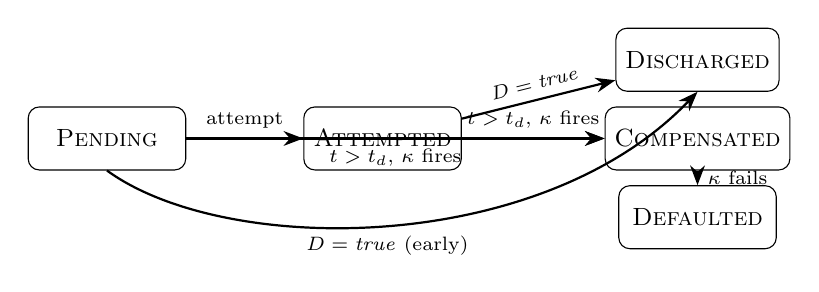
\begin{tikzpicture}[
    state/.style={draw, rounded corners, minimum width=2cm, minimum height=0.8cm, font=\small},
    arr/.style={-{Stealth[length=2.5mm]}, thick},
  ]
  \node[state] (P) at (0,0) {\textsc{Pending}};
  \node[state] (A) at (3.5,0) {\textsc{Attempted}};
  \node[state] (D) at (7.5,1) {\textsc{Discharged}};
  \node[state] (C) at (7.5,0) {\textsc{Compensated}};
  \node[state] (F) at (7.5,-1) {\textsc{Defaulted}};

  \draw[arr] (P) -- node[above, font=\scriptsize] {attempt} (A);
  \draw[arr] (A) -- node[above, font=\scriptsize, sloped] {$D = \mathit{true}$} (D);
  \draw[arr] (A) -- node[above, font=\scriptsize] {$t > t_d$, $\kappa$ fires} (C);
  \draw[arr] (P) -- node[below, font=\scriptsize, sloped] {$t > t_d$, $\kappa$ fires} (C);
  \draw[arr] (P.south) .. controls (1.5,-1.5) and (5.5,-1.5) .. node[below, font=\scriptsize] {$D = \mathit{true}$ (early)} (D.south);
  \draw[arr] (C) -- node[right, font=\scriptsize] {$\kappa$ fails} (F);
\end{tikzpicture}
\end{center}

\noindent Terminal states are \textsc{Discharged}, \textsc{Compensated}, and \textsc{Defaulted}. No obligation leaves a terminal state.

%----------------------------------------------------------------------
\subsubsection{Obligation Taxonomy}
\label{sec:obligation-taxonomy}
%----------------------------------------------------------------------

Table~\ref{tab:obligation-types} classifies all obligation types in the framework by trigger mechanism and scope.

\begin{table}[ht]
\centering
\small
\begin{tabular}{l l l l}
\toprule
\textbf{Obligation type} & \textbf{Scope} & \textbf{Trigger} & \textbf{Compensation $\kappa$} \\
\midrule
\multicolumn{4}{l}{\textit{Deterministic-date (timer at registration)}} \\
Bond coupon & Unit & Timer at coupon date & Default event \\
Option expiry & Unit & Timer at termination date & N/A (auto-expire) \\
IRS reset & Unit & Timer at reset date & Default event \\
Futures daily VM & Unit & Cron at exchange EOD & Position liquidation \\
SBL term loan return & Unit & Timer at maturity & Buy-in (GMSLA~9.3) \\
\midrule
\multicolumn{4}{l}{\textit{Event-triggered (timer at event time)}} \\
SBL recall return & Unit & Recall signal & Buy-in (GMSLA~9.3) \\
SBL manuf.\ dividend & Unit & Corp.\ action record date & Cost attribution \\
SBL collateral subst. & Unit & Demand / eligibility change & Shortfall escalation \\
CSA VM delivery & Agreement & Margin call computation & Close-out netting (ISDA) \\
CSA IM delivery & Agreement & Regulatory schedule & Close-out netting \\
Collateral substitution & Agreement & Schedule amendment & Close-out netting \\
SBL collateral top-up & Unit & MTM threshold breach & Recall / default \\
Close-out netting & Agreement & Default event & Waterfall / loss alloc. \\
\midrule
\multicolumn{4}{l}{\textit{Regulatory}} \\
SFTR report & Unit & SBL lifecycle event & Regulatory penalty \\
SLATE report & Unit & SBL lifecycle event & Regulatory penalty \\
EMIR report & Unit & Trade/lifecycle event & Regulatory penalty \\
Settlement instruction & Unit & Settlement-type transaction & Failed settlement \\
\bottomrule
\end{tabular}
\caption{Obligation types by trigger mechanism and scope. Deterministic-date obligations are scheduled at unit registration. Event-triggered obligations are created when the triggering event is processed. Regulatory obligations are created alongside the business event.}
\label{tab:obligation-types}
\end{table}

%----------------------------------------------------------------------
\subsubsection{The Obligation Store}
\label{sec:obligation-store}
%----------------------------------------------------------------------

\begin{definition}[Obligation Store]
\label{def:obligation-store}
The \emph{obligation store}~$\mathcal{O}$ is an append-only registry of obligations. Obligations are added atomically as part of the transaction that creates the triggering event. Obligation state transitions are recorded in the event log (Section~\ref{sec:implementation}, Layer~1) as state-only transactions, preserving the audit trail and supporting time travel (Property~6, Section~\ref{sec:intro}).
\end{definition}

\noindent The obligation store is not a separate system; it is a view over the event log, filtered to obligation-typed entries. Like the Unit Store (Section~\ref{sec:unit-store}), it is a registry that manages a typed universe of objects with lifecycle state.

%----------------------------------------------------------------------
\subsubsection{Obligation Registration}
\label{sec:obligation-registration}
%----------------------------------------------------------------------

Obligations are registered through two channels, corresponding to the two trigger regimes:

\paragraph{At unit registration (deterministic-date obligations).}
When a unit is registered (Section~\ref{sec:unit-registration}), the lifecycle function extracts obligation dates from the CDM \texttt{EconomicTerms} (coupon schedule, reset schedule, termination date) and registers one obligation per date. These obligations map one-to-one to the Temporal timers described in Section~\ref{sec:temporal-scheduler}. The registration makes explicit what was previously implicit: each timer corresponds to an obligation with a defined discharge predicate and compensation action.

\paragraph{At event processing (event-triggered obligations).}
When a lifecycle event creates a new obligation---a recall signal, a margin call computation, a collateral eligibility change---the lifecycle function includes the obligation in its return value alongside the moves and state deltas. The executor commits the obligation registration atomically with the triggering event. The obligation workflow (Section~\ref{sec:obligation-workflow}) is spawned as a post-commit action.

\begin{principle}[Obligation Completeness]
\label{princ:obligation-completeness}
A lifecycle function that processes an obligation-creating event must include the obligation in its output. A lifecycle function that omits a required obligation is incorrect, regardless of whether the moves it produces are valid.
\end{principle}

\noindent This principle is enforceable by property-based testing: for each event type in the obligation taxonomy (Table~\ref{tab:obligation-types}), the test generator produces events of that type and verifies that the lifecycle function's output includes a non-empty obligation list. The CDM event type enumeration (Section~\ref{sec:invariants}) bounds the test space.

%----------------------------------------------------------------------
\subsubsection{The Obligation Workflow}
\label{sec:obligation-workflow}
%----------------------------------------------------------------------

Each obligation spawns a Temporal workflow or is tracked by the existing unit/agreement lifecycle workflow with an internal obligation register. The pattern is uniform:

\begin{lstlisting}
ObligationWorkflow(obligation):
    o = obligation
    discharge_ch = workflow.GetSignalChannel("discharge_" + o.id)
    selector = workflow.NewSelector()

    selector.AddReceive(discharge_ch, func(signal):
        if o.discharge_predicate(signal.ledger_state):
            await RecordObligationState(o.id, DISCHARGED)
            return  -- workflow completes
        else:
            await RecordObligationState(o.id, ATTEMPTED)
            -- remain in loop, wait for correct discharge or deadline
    )

    selector.AddTimer(o.deadline, func():
        state = await CheckLedgerState(o.source)
        if o.discharge_predicate(state):
            await RecordObligationState(o.id, DISCHARGED)
            return
        -- Deadline passed without discharge. Fire compensation.
        compensation_tx = await o.compensation_action(o)
        result = await ExecutorCommit(compensation_tx)
        if result.success:
            await RecordObligationState(o.id, COMPENSATED)
        else:
            await RecordObligationState(o.id, DEFAULTED)
            await RaiseDefaultEvent(o.source)
    )

    selector.Select()
\end{lstlisting}

\noindent The workflow ID is derived deterministically from \texttt{o.id}, providing natural idempotency: Temporal rejects duplicate starts.

For obligations managed within an existing lifecycle workflow (e.g., the SBL loan workflow in Section~\ref{sec:sbl-lifecycle-workflow}), the pattern is the same---a selector with a discharge signal channel and a deadline timer---but embedded within the parent workflow rather than spawned as a separate child.

%----------------------------------------------------------------------
\subsubsection{Liveness Invariants}
\label{sec:obligation-invariants}
%----------------------------------------------------------------------

\begin{invariant}[P21---Obligation Liveness]
\label{inv:obligation-liveness}
For every obligation $o \in \mathcal{O}$ registered at time $t_0$ with deadline $t_d$:
\[
\forall\, t > t_d : \quad o.\mathit{state} \in \{\textsc{Discharged},\; \textsc{Compensated},\; \textsc{Defaulted}\}
\]
No obligation persists in state \textsc{Pending} or \textsc{Attempted} beyond its deadline.
\end{invariant}

\begin{invariant}[P22---Obligation Conservation]
\label{inv:obligation-conservation}
Every discharging move set for obligation~$o$ satisfies the conservation law $Q(u) = 0$ (Invariant~1). Every compensation move set satisfies conservation. The obligation mechanism does not bypass the executor.
\end{invariant}

\begin{invariant}[P23---Obligation Idempotency]
\label{inv:obligation-idempotency}
Discharging the same obligation twice (by $o.\mathit{id}$) has no incremental effect. The discharge predicate~$D$ is checked before emitting moves; if already satisfied, no moves are produced. This composes with transaction-ID idempotency (Invariant~5) and lifecycle idempotency (Invariant~6).
\end{invariant}

%----------------------------------------------------------------------
\subsubsection{Proof of Liveness}
\label{sec:liveness-proof}
%----------------------------------------------------------------------

\begin{theorem}[Obligation Liveness]
\label{thm:obligation-liveness}
Under the Executor + Temporal + Obligation Store architecture, Invariant~\ref{inv:obligation-liveness} (P21) holds: no obligation persists in state \textsc{Pending} beyond its deadline.
\end{theorem}

\begin{proof}
The argument is a chain of five lemmas.

\medskip
\noindent\textbf{Lemma~1 (Registration completeness).} Every obligation-creating event registers an obligation in~$\mathcal{O}$.

\textit{Enforcement}: Principle~\ref{princ:obligation-completeness} makes obligation registration part of the lifecycle function's output contract. The executor commits obligations atomically with the triggering event. Registration completeness is verified by property-based testing: for each obligation-creating event type, the generator produces events and the postcondition verifies that the obligation list is non-empty.

\medskip
\noindent\textbf{Lemma~2 (Workflow creation).} Every obligation in~$\mathcal{O}$ is managed by a Temporal workflow with a timer at~$t_d$.

\textit{Enforcement}: The executor's post-commit hook spawns the obligation workflow. The workflow ID is derived deterministically from $o.\mathit{id}$, so Temporal's duplicate-start rejection prevents double-spawning.

\medskip
\noindent\textbf{Lemma~3 (Timer durability).} The timer at~$t_d$ is persisted in Temporal's database and survives server restarts, worker deployments, version upgrades, and data centre failovers.

\textit{Enforcement}: This is a property of the Temporal SDK and server, as described in Section~\ref{sec:temporal-why}.

\medskip
\noindent\textbf{Lemma~4 (Timer fires).} The timer fires at~$t_d$.

\textit{Enforcement}: Temporal's core durable-execution guarantee. \textit{Prerequisite}: the Temporal cluster is available at~$t_d$. Cluster availability is an operational prerequisite, not a framework property. Temporal's multi-region replication (Section~\ref{sec:temporal-taskqueues}) mitigates but does not eliminate this dependency.

\medskip
\noindent\textbf{Lemma~5 (Handler totality).} When the timer fires, the handler transitions~$o$ out of \textsc{Pending}.

\textit{Enforcement}: The handler code (Section~\ref{sec:obligation-workflow}) is total over its inputs. It checks the discharge predicate~$D$. If $D = \mathit{true}$, the obligation is marked \textsc{Discharged}. If $D = \mathit{false}$, the compensation action~$\kappa$ is invoked. If $\kappa$ succeeds, the obligation is marked \textsc{Compensated}. If $\kappa$ fails, the obligation is marked \textsc{Defaulted} and a default event is raised. Every branch terminates in a terminal state.

\medskip
\noindent\textbf{Composition.} For any obligation~$o$ registered at~$t_0$ with deadline~$t_d$:
\begin{itemize}[nosep]
\item By Lemma~1, $o \in \mathcal{O}$.
\item By Lemma~2, a workflow exists for~$o$ with a timer at~$t_d$.
\item By Lemma~3, the timer is durable.
\item By Lemma~4, the timer fires at~$t_d$ (assuming cluster availability).
\item By Lemma~5, the handler transitions~$o$ to a terminal state.
\end{itemize}
Therefore, for all $t > t_d$: $o.\mathit{state} \in \{\textsc{Discharged},\; \textsc{Compensated},\; \textsc{Defaulted}\}$.
\end{proof}

\paragraph{Consistency with existing invariants.}
P22 (obligation conservation) follows from P1 (conservation) and the executor exclusivity principle (Section~\ref{sec:lifecycle}, \S7.7.1): every discharging and compensating move passes through the executor, which validates $Q(u) = 0$ before committing. P23 (obligation idempotency) composes with P5 (transaction-ID idempotency) and P6 (lifecycle idempotency) via the three-layer idempotency chain (Section~\ref{sec:temporal-idempotency}): the obligation ID is part of the transaction source metadata, the discharge predicate prevents re-emission, and the transaction ID prevents re-commitment.

%----------------------------------------------------------------------
\subsubsection{The Liveness--Safety Composition (Revised)}
\label{sec:liveness-safety-revised}
%----------------------------------------------------------------------

Section~\ref{sec:temporal-scheduler} established the liveness--safety composition for deterministic-date obligations. With the obligation type, the composition extends to all obligations:

\begin{center}
\small
\begin{tabular}{l l l}
\toprule
\textbf{Property} & \textbf{Guarantee source} & \textbf{Scope} \\
\midrule
Every obligation fires & Temporal durable timer (Lemma~4) & All obligations \\
No obligation fires twice & Idempotency chain (P5, P6, P23) & All obligations \\
Discharge preserves conservation & Executor (P1, P22) & All obligations \\
Handler reaches terminal state & Workflow totality (Lemma~5) & All obligations \\
\bottomrule
\end{tabular}
\end{center}

\noindent The combination resolves the remaining piece of the liveness gap identified in v7.4 (Section~\ref{sec:conclusion}): not only do deterministic-date events fire, but \emph{every obligation---including those created dynamically during the lifecycle---is tracked, timed, and resolved}.

%----------------------------------------------------------------------
\subsubsection{Worked Example: CSA Variation Margin Call}
\label{sec:obligation-example-csa}
%----------------------------------------------------------------------

Alice and Bob have a CSA governing five IRS trades with threshold \$500{,}000 and minimum transfer amount \$250{,}000.

\paragraph{Step~1: Margin call computation.} The daily \texttt{CSAMarginWorkflow} (Section~\ref{sec:lifecycle-workflows}) computes aggregate mark-to-market: exposure = \$2.3M in Alice's favour. Required margin: $\max(0, |\$2.3\text{M}| - \$500\text{K}) = \$1.8\text{M}$. Since $\$1.8\text{M} \geq \$250\text{K}$ (MTA), a margin call is generated.

\paragraph{Step~2: Obligation registration.} The margin call transaction registers an obligation:
\begin{lstlisting}
Obligation(
    id:            "CSA-AB-20260328-VM",
    type:          CSA_VARIATION_MARGIN,
    source:        CSA-AB,
    deadline:      2026-03-31T17:00 (T+1, next business day COB),
    discharge:     Bob.coll_post(USD, CSA-AB) increased by >= 1,800,000,
    compensation:  CSA_CloseOutNetting(CSA-AB)
)
\end{lstlisting}

\noindent The obligation is committed atomically with the margin call event. The obligation workflow starts with a timer at 2026-03-31T17:00.

\paragraph{Step~3a: Discharge (happy path).} Bob delivers \$1.8M before the deadline. The delivery is a conservation-preserving move submitted to the executor:

\begin{lstlisting}
Move(from: w_Bob, to: w_Alice_coll, unit: USD,
     quantity: 1,800,000, source: "CSA-AB-VM-20260328")
\end{lstlisting}

\noindent The discharge signal is sent to the obligation workflow. The handler checks the discharge predicate: Bob's collateral balance under CSA-AB has increased by \$1.8M. Predicate satisfied. Obligation $\to$ \textsc{Discharged}.

\paragraph{Step~3b: Compensation (failure path).} Bob does not deliver by the deadline. The timer fires at 2026-03-31T17:00. The handler checks the discharge predicate---not satisfied. Compensation fires: the \texttt{CSA\_CloseOutNetting} function terminates all five IRS trades, computes close-out values per the ISDA Master Agreement, and emits a single net settlement move. All moves pass through the executor. Conservation preserved (P22). Obligation $\to$ \textsc{Compensated}.

\paragraph{Conservation verification (discharge path).}
\begin{align*}
\Delta\, w_{\mathrm{Bob}}(\text{USD})[\mathrm{own}] &= -1{,}800{,}000 \\
\Delta\, w_{\mathrm{Alice}}(\text{USD})[\mathrm{coll\_recv}] &= +1{,}800{,}000 \\
Q(\text{USD}) &= -1{,}800{,}000 + 1{,}800{,}000 = 0 \;\checkmark
\end{align*}

%----------------------------------------------------------------------
\subsubsection{Worked Example: SBL Collateral Substitution}
\label{sec:obligation-example-sbl}
%----------------------------------------------------------------------

Lender demands substitution: bond XYZ (ISIN DE000...) is no longer eligible per the updated collateral schedule.

\paragraph{Step~1: Obligation registration.} The collateral eligibility check identifies the ineligible collateral and registers (IBP references throughout denote clauses of the ISLA Best Practice Handbook~\cite{isla-ibp}):
\begin{lstlisting}
Obligation(
    id:            "SBL-L123-SUBST-20260328",
    type:          SBL_COLLATERAL_SUBSTITUTION,
    source:        loan L123,
    deadline:      2026-03-28T15:30 (1h before DVP cut-off, IBP-170),
    discharge:     new eligible collateral posted AND old released,
    compensation:  CollateralShortfallEscalation(L123)
)
\end{lstlisting}

\paragraph{Step~2: Discharge (happy path).} The borrower delivers German Bund as replacement. The substitution is a transaction of four moves, each satisfying the Single-Coordinate Move Principle (Principle~\ref{princ:single-coord}):

\begin{lstlisting}
tau_subst = Transaction(type = SETTLEMENT):
  Move 1: Borrower coll_post(XYZ) -= old_amt   [coll_post, XYZ]
  Move 2: Lender   coll_recv(XYZ) -= old_amt   [coll_recv, XYZ]
  Move 3: Borrower coll_post(BUND) += new_amt   [coll_post, BUND]
  Move 4: Lender   coll_recv(BUND) += new_amt   [coll_recv, BUND]
\end{lstlisting}

\noindent Conservation per unit: $\Delta Q(\text{XYZ}) = -\mathit{old\_amt} + \mathit{old\_amt} = 0$; $\Delta Q(\text{BUND}) = \mathit{new\_amt} - \mathit{new\_amt} = 0$. Obligation $\to$ \textsc{Discharged}.

\paragraph{Step~3: Compensation (failure path).} The cut-off passes without delivery. The timer fires. \texttt{CollateralShortfallEscalation}:
\begin{enumerate}[nosep]
\item Marks loan L123 as collateral-deficient in the SBL unit state.
\item Raises an exposure breach notification.
\item If the breach persists beyond the GMSLA grace period, triggers recall or default per GMSLA~$\S$10.
\end{enumerate}
Obligation $\to$ \textsc{Compensated}.

%----------------------------------------------------------------------
\subsubsection{Relationship to SBL Invariants}
\label{sec:obligation-sbl-relationship}
%----------------------------------------------------------------------

The obligation liveness invariant (P21) strengthens the SBL-specific invariants (P11--P20, Section~\ref{sec:sbl-invariants}) by providing the temporal guarantee that underpins them:

\begin{itemize}[nosep]
\item \textbf{P13 (Collateral Sufficiency)}: P21 guarantees that collateral top-up obligations are resolved by their deadline---either the borrower delivers (collateral restored) or compensation fires (recall/default). Without P21, P13 could be violated by an untracked collateral call that is simply never followed up.

\item \textbf{P16 (SFTR Completeness)}: Each reportable SBL event creates a regulatory reporting obligation. P21 guarantees that the reporting workflow fires before the T+1 deadline, or a regulatory escalation is triggered.

\item \textbf{P18 (Lender Ownership Invariance)}: P21 ensures that recall obligations are resolved, preventing the indefinite state where shares are on loan past a recall deadline without either return or buy-in.
\end{itemize}

%----------------------------------------------------------------------
\subsubsection{Property-Based Testing for Obligations}
\label{sec:obligation-testing}
%----------------------------------------------------------------------

The obligation type extends the property-based testing framework (Section~\ref{sec:invariants}) with three additional test properties:

\begin{enumerate}\setcounter{enumi}{10}
\item \textbf{Obligation registration completeness.} Generator: random lifecycle events of obligation-creating types (Table~\ref{tab:obligation-types}). Postcondition: the lifecycle function's output includes a non-empty obligation list with valid deadline, discharge predicate, and compensation action.

\item \textbf{Obligation discharge conservation.} Generator: random obligations with random discharge move sets. Postcondition: every discharge move set satisfies $Q(u) = 0$.

\item \textbf{Obligation handler totality.} Generator: random obligation states $\times$ \{discharge-before-deadline, no-discharge-by-deadline, compensation-success, compensation-failure\}. Postcondition: the handler reaches a terminal state in every case.
\end{enumerate}

\noindent The CDM event type enumeration bounds the obligation-creating event space, making coverage structurally complete (Section~\ref{sec:invariants}, \S11.4). For each CDM \texttt{EventIntentEnum} value that creates an obligation, the test generator produces the event and verifies that the obligation is registered, tracked, and resolved.

%----------------------------------------------------------------------
\subsubsection{Assumptions and Limitations}
\label{sec:obligation-limitations}
%----------------------------------------------------------------------

The proof of Theorem~\ref{thm:obligation-liveness} depends on four assumptions:

\begin{enumerate}
\item \textbf{Temporal cluster availability at~$t_d$.} If the Temporal cluster is unavailable when the deadline timer should fire, the timer is delayed until cluster recovery. Liveness holds \emph{eventually} (after recovery), not instantaneously at~$t_d$. Temporal's multi-region replication and the cluster operations described in Section~\ref{sec:temporal-taskqueues} mitigate this risk but cannot eliminate it.

\item \textbf{Executor availability.} Compensation moves must be committed by the executor. If the executor is unavailable, Temporal retries the activity per the retry policy (Section~\ref{sec:temporal-timeouts}). The obligation remains in \textsc{Pending} until the executor recovers. This is a bounded delay, not a permanent failure, assuming the executor's transient-failure retries eventually succeed.

\item \textbf{External counterparty cooperation for discharge.} Some discharge conditions require external action (counterparty delivers margin, borrower returns securities). The framework cannot compel external actors. Discharge depends on external signals; compensation is the contractual fallback when external cooperation fails.

\item \textbf{Lifecycle function correctness.} Lemma~1 assumes that lifecycle functions register all required obligations. This is a correctness requirement on the smart contract author, enforceable by property-based testing (Property~11 above) but not by construction in an untyped implementation. In a typed implementation, the lifecycle function's return type can include a mandatory obligation list for obligation-creating event types, making omission a compile-time error.
\end{enumerate}

\noindent These assumptions are consistent with the framework's existing boundary (Section~\ref{sec:scope-limitations}): the framework guarantees correctness for activity within the ledger, given infrastructure availability and correct smart contracts. External actors and infrastructure availability are outside the ledger boundary.

\clearpage
%==============================================================================
\section{Generalised Positions and Securities Borrowing and Lending}
\label{sec:gpm}
%==============================================================================

The scalar model developed in Sections~\ref{sec:ledger}--\ref{sec:invariants}---one number per (wallet, unit) pair (or a six-coordinate vector when the generalised position model applies; for non-lendable instruments, this degenerates to a scalar)---is sufficient for buy/sell/exercise workflows that cover the vast majority of instruments. It is \emph{not} sufficient for activities where ownership and possession diverge: securities lending, repo, pledged collateral, or any instrument requiring lifecycle-rich position tracking beyond a net quantity. This section shows where the scalar model breaks, introduces a vector generalisation that resolves the failure, and develops Securities Borrowing and Lending (SBL) as a native application of the framework. Repo, collateral management beyond SBL, and novation/partial assignment workflows are identified as open problems (Section~\ref{sec:conclusion}).

%----------------------------------------------------------------------
\subsection{Motivation: Where the Scalar Model Breaks}
\label{sec:scalar-breaks}
%----------------------------------------------------------------------

\noindent\textbf{The simplest possible ledger.} Alice buys 1{,}000 shares of Vodafone (VOD) for GBP~200{,}000. Her wallet balance is:
\[
w_{\mathrm{Alice}}(\text{VOD}) = 1{,}000
\]
This is a single number, and it is all we need. For cash, equities, derivatives, swaps, and all other instruments that are not lent or borrowed, the scalar model is complete.

\medskip
\noindent\textbf{Where the scalar model breaks.} Alice lends 400~VOD to Bob. In a scalar model, three attempts all fail:

\begin{enumerate}[nosep]
\item \emph{Transfer the shares:} $w_{\mathrm{Alice}}(\text{VOD}) = 600$, $w_{\mathrm{Bob}}(\text{VOD}) = 400$. Conservation holds, but Alice's PnL drops by 40\%---wrong, because under IFRS~9 paragraph~3.2.6, the lender does not derecognise lent securities.
\item \emph{Do not transfer:} $w_{\mathrm{Alice}}(\text{VOD}) = 1{,}000$, $w_{\mathrm{Bob}}(\text{VOD}) = 0$. Bob possesses 400~shares but has no record of them.
\item \emph{Credit both:} $w_{\mathrm{Alice}}(\text{VOD}) = 1{,}000$, $w_{\mathrm{Bob}}(\text{VOD}) = 400$. Total = 1{,}400, but the external world holds only 1{,}000. Conservation is violated.
\end{enumerate}

\noindent The root cause: a scalar balance cannot encode two distinct operational states simultaneously. After the loan, Alice's relationship with VOD has two aspects: 600~shares available and 400~shares on loan. The physical analogy is instructive: lending a car does not transfer ownership. ``On-loan'' is a coordinate because ``lend'' is a physical action that changes operational status without changing ownership.

%----------------------------------------------------------------------
\subsection{The Generalised Coordinate Vector}
\label{sec:position-vector}
%----------------------------------------------------------------------

A coordinate is a stored quantity that passes the \emph{physical-action test}: there exists a distinct physical action that modifies this coordinate and only this coordinate. A quantity that is fully determined by other coordinates via an algebraic identity is a \emph{projection}---computed on read, never stored, never written to by a move.

\begin{principle}[Single-Coordinate Move]
\label{princ:single-coord}
An atomic move modifies exactly one coordinate of one unit in the position vectors of the entities it connects. One move, one coordinate, one unit, two entities (source and destination). A move is the smallest possible state change. Any operation that requires multiple coordinate changes is a \emph{transaction}---a list of moves executed atomically.
\end{principle}

\noindent This principle is consistent with the scalar core (Sections~\ref{sec:ledger}--\ref{sec:invariants}): in the scalar model, a move modifies one wallet (which has one coordinate) per entity. The principle makes the same guarantee explicit in the vector model.

\begin{definition}[Position Vector]
\label{def:position-vector-gpm}
For an entity~$e$ and unit~$u$, the \emph{position vector} is an element of $\mathbb{R}^6$:
\[
\vec{w}_e(u) = \bigl(
  \underbrace{w^{\mathrm{own}}_e(u)}_{\text{own}},\;
  \underbrace{w^{\mathrm{onloan}}_e(u)}_{\text{onloan}},\;
  \underbrace{w^{\mathrm{borr}}_e(u)}_{\text{borr}},\;
  \underbrace{w^{\mathrm{coll\text{-}post}}_e(u)}_{\text{coll\_post}},\;
  \underbrace{w^{\mathrm{coll\text{-}recv}}_e(u)}_{\text{coll\_recv}},\;
  \underbrace{w^{\mathrm{coll\text{-}rehyp}}_e(u)}_{\text{coll\_rehyp}}
\bigr)
\]
Each coordinate passes the physical-action test:
\begin{itemize}[nosep]
\item $\mathrm{own}$: economic ownership. Modified by buy/sell. Can be negative (short positions). Drives PnL.
\item $\mathrm{onloan}$: securities lent out. Modified by lend/recall-return. The lender retains economic ownership.
\item $\mathrm{borr}$: borrowed shares received (the obligation count---must be returned). Modified by borrow-receive/return-to-lender. Non-negative. Does not change when the borrower sells.
\item $\mathrm{coll\_post}$: collateral delivered to a lender or triparty agent. Modified by post-collateral/release.
\item $\mathrm{coll\_recv}$: collateral held from the borrower. Modified by receive-collateral/release.
\item $\mathrm{coll\_rehyp}$: non-cash collateral re-used by the collateral taker. Modified by rehypothecate/recall. Tracked for SFTR Article~15 compliance.
\end{itemize}
\end{definition}

\noindent Available inventory and pending settlement state are projections, not stored coordinates: they fail the physical-action test and are fully determined by the six coordinates above.

\begin{definition}[Available Inventory (Projection)]
\label{def:avail-projection}
For all entities~$e$ and lendable units~$u$, available inventory is computed on read:
\[
\mathrm{avail}(e,u) \;\stackrel{\mathrm{def}}{=}\; \vec{w}_e(u)[\mathrm{own}] - \vec{w}_e(u)[\mathrm{onloan}] + \vec{w}_e(u)[\mathrm{borr}]
\]
which reads: \emph{what you can trade = what you own, minus what you've lent out, plus what you've borrowed.}

Because $\mathrm{avail}$ is never stored, the identity holds by definition---there is no stored value that can drift out of sync with the coordinates that determine it.
\end{definition}

\begin{remark}[Special cases]
\hfill
\begin{itemize}[nosep]
\item \textbf{Pure holder/lender} ($\mathrm{borr} = 0$): reduces to $\mathrm{avail} = \mathrm{own} - \mathrm{onloan}$.
\item \textbf{Non-SBL entity} (all SBL coordinates zero): reduces to $\mathrm{avail} = \mathrm{own}$.
\item \textbf{Borrower who sold $Q$ of $N$ borrowed shares} ($\mathrm{own} = -Q$, $\mathrm{borr} = N$): $\mathrm{avail} = -Q - 0 + N = N - Q$.
\end{itemize}
\end{remark}

\noindent\textbf{Why \texttt{own} is the first coordinate and not a projection.} Four reasons: (1)~PnL computation is a direct coordinate lookup---no summation, no regime-dependent projection logic at read time; (2)~for non-lendable instruments (the vast majority), only $\mathrm{own}$ is non-zero, making the vector equivalent to a scalar; (3)~$\mathrm{own}$ cannot be derived from the five operational coordinates alone (proof: two states with identical operational vectors but different $\mathrm{own}$ values exist whenever a borrower has sold some but not all borrowed shares); (4)~every move that changes $\mathrm{own}$ (buy/sell) is a distinct physical action that does not modify any other coordinate.

\begin{proposition}[Conservation in the Generalised Model]
\label{prop:gpm-conservation}
Each move subtracts $q$ from one (entity, coordinate) slot and adds $q$ to another. The algebraic sum across all slots is preserved by construction---this follows directly from the $\mathrm{src} \mathbin{{-}{=}} q;\; \mathrm{dst} \mathbin{{+}{=}} q$ pattern of the core framework (Section~\ref{sec:ledger}).

For the meaningful conservation check---total physical quantity of each unit---substitute the $\mathrm{avail}$ projection into the sum. Expanding all six coordinates:
\[
\sum_{e \in \mathcal{E}} \bigl( \vec{w}_e(u)[\mathrm{own}] + \vec{w}_e(u)[\mathrm{onloan}] + \vec{w}_e(u)[\mathrm{borr}] + \vec{w}_e(u)[\mathrm{coll\_post}] + \vec{w}_e(u)[\mathrm{coll\_recv}] + \vec{w}_e(u)[\mathrm{coll\_rehyp}] \bigr) = 0.
\]
For each unit~$u$, the lender's $+\mathrm{onloan}$ and the per-relationship virtual wallet's $-\mathrm{onloan}$ contra-entry cancel in the global sum, leaving five terms per real entity:
\[
\sum_{e \in \mathcal{E}} \bigl( \vec{w}_e(u)[\mathrm{own}] + \vec{w}_e(u)[\mathrm{borr}] + \vec{w}_e(u)[\mathrm{coll\_post}] + \vec{w}_e(u)[\mathrm{coll\_recv}] + \vec{w}_e(u)[\mathrm{coll\_rehyp}] \bigr) = 0
\]
where $\mathcal{E}$ includes both real entities and virtual wallets. This is a cleaner equation than an eight-coordinate formulation: five terms per entity instead of six, and the cancellation of $\mathrm{onloan}$ reflects the physical reality that lent shares are not double-counted (they appear once as the borrower's $\mathrm{borr}$).
\end{proposition}

\medskip
\noindent\textbf{Portfolio value using the \texttt{own} coordinate.} For entity~$e$:
\[
V_e(t) = \sum_{u \in \mathcal{U}} \vec{w}_e(u)[\mathrm{own}] \cdot P_t(u)
\]
This is the scalar formula from Section~\ref{sec:valuation} with $\mathrm{own}$ replacing the scalar balance. No projections, no filtering, no conditional logic.

\medskip
\noindent\textbf{Settlement timing and in-flight collateral.}
Standard buy/sell trades use trade-date accounting: when Alice buys 500~AAPL at time~$T$, her position vector is immediately updated to $\vec{w}_{\mathrm{Alice}}(\text{AAPL}) = (500,\; 0,\; 0,\; 0,\; 0,\; 0)$. The unsettled delivery obligation lives in the virtual wallet (the custodian contra-entry).

For SBL prepay collateral (IBP-177; IBP references throughout denote clauses of the ISLA Best Practice Handbook~\cite{isla-ibp}), where collateral is instructed before the loan settles, the in-flight collateral is modelled as a virtual-wallet entry---exactly as unsettled buy/sell obligations are handled. Upon settlement confirmation, the virtual-wallet entry resolves to a move writing $\mathrm{coll\_recv}$ (for the lender) or $\mathrm{coll\_post}$ (for the borrower). The custodian reconciliation formula becomes: $\mathrm{avail}(L,u) + \vec{w}_L(u)[\mathrm{onloan}] + \mathrm{inflight}(L,u) \stackrel{?}{=} \text{Custodian depot}(u)$, where $\mathrm{inflight}$ is a virtual-wallet query. Substituting the $\mathrm{avail}$ projection and simplifying: $\vec{w}_L(u)[\mathrm{own}] + \vec{w}_L(u)[\mathrm{borr}] + \mathrm{inflight}(L,u) \stackrel{?}{=} \text{Custodian depot}(u)$.

%----------------------------------------------------------------------
\subsection{Graceful Degeneration to the Scalar Model}
\label{sec:degeneration}
%----------------------------------------------------------------------

\begin{remark}[Non-lendable instruments]
For non-lendable instruments---OTC derivatives, listed options and futures, FX forwards, credit derivatives, cash---only the $\mathrm{own}$ coordinate is non-zero. The vector degenerates to:
\[
\vec{w}_e(u) = (q,\; 0,\; 0,\; 0,\; 0,\; 0)
\]
where $q = \vec{w}_e(u)[\mathrm{own}]$. The six-coordinate structure adds no cognitive overhead for these instruments. The PnL formula $V_e(t) = \sum_u \vec{w}_e(u)[\mathrm{own}] \cdot P_t(u)$ reduces to a single coordinate lookup per unit. The $\mathrm{avail}$ projection yields $\mathrm{own} - 0 + 0 = q$. The scalar model from Sections~\ref{sec:ledger}--\ref{sec:invariants} is recovered exactly.
\end{remark}

\noindent\textbf{The collapse property.} For entities not engaged in securities lending, only the $\mathrm{own}$ coordinate is non-zero. Every other coordinate is zero. The model collapses to a scalar: $\vec{w}_e(u)[\mathrm{own}] = q$, a single number per (entity, unit) pair. The generalisation is invisible when not needed.

%----------------------------------------------------------------------
\subsection{The Lending Resolution: Named Wallets}
\label{sec:named-wallets}
%----------------------------------------------------------------------

Returning to Alice's loan of 400~VOD to Bob. After the loan, Alice's position vector is:
\[
\vec{w}_{\mathrm{Alice}}(\text{VOD}) = (1000,\; 400,\; 0,\; 0,\; 0,\; 0)
\]
The first coordinate is still 1{,}000---lending does not change ownership. The $\mathrm{avail}$ projection: $1000 - 400 + 0 = 600$. \checkmark

Bob has:
\[
\vec{w}_{\mathrm{Bob}}(\text{VOD}) = (0,\; 0,\; 400,\; 0,\; 0,\; 0)
\]
Bob's $\mathrm{own}$ is zero---borrowed is not ownership. The $\mathrm{avail}$ projection: $0 - 0 + 400 = 400$. A per-relationship virtual wallet absorbs the delivery contra-entry: $w^{\mathrm{virtual}}_{A \leftrightarrow B}(\text{VOD}) = -400$.

Conservation holds across all wallets. Using the five-term conservation equation from Proposition~\ref{prop:gpm-conservation}:
\[
\underbrace{1000}_{\mathrm{own}_A} + \underbrace{0}_{\mathrm{borr}_A} + \underbrace{0}_{\mathrm{own}_B} + \underbrace{400}_{\mathrm{borr}_B} + \underbrace{(-400)}_{\text{virtual}_{A \leftrightarrow B}} + \underbrace{(-1000)}_{\text{custodian}} = 0. \;\checkmark
\]
\noindent (Note: the first four terms are coordinates from entity position vectors; the last two are scalar virtual-wallet balances from the core framework. The $\mathrm{onloan}$ terms do not appear---they cancel algebraically when the $\mathrm{avail}$ projection is substituted.)
Alice's PnL correctly reflects 1{,}000~shares: read $\vec{w}_{\mathrm{Alice}}(\text{VOD})[\mathrm{own}] = 1{,}000$.

\noindent\textbf{Reclassification vs.\ transfer.} Under the Single-Coordinate Move Principle, a \emph{reclassification} is a transaction of two moves within the same entity: one coordinate decreases, another increases (e.g., rehypothecation: $\mathrm{coll\_recv}$ decreases, $\mathrm{coll\_rehyp}$ increases). A \emph{transfer} is a move between different entities. The move primitive is identical in both cases; the semantic distinction arises from the entity identities. Lending writes $\mathrm{onloan}$ for the lender---the decrease in $\mathrm{avail}$ is computed on read, not written.

%----------------------------------------------------------------------
\subsection{Analytical Projections and Encumbrance}
\label{sec:projections}
%----------------------------------------------------------------------

\begin{definition}[Projections (Computed on Read)]
\label{def:projections}
All projections are functions of the six stored coordinates. None is stored; none is written to by a move.
\begin{align*}
\mathrm{avail}(e, u) &= \vec{w}_e(u)[\mathrm{own}] - \vec{w}_e(u)[\mathrm{onloan}] + \vec{w}_e(u)[\mathrm{borr}] && \text{tradeable inventory} \\
\mathrm{possess}(e, u) &= \mathrm{avail}(e,u) + \vec{w}_e(u)[\mathrm{coll\_recv}] && \text{physical custody} \\
\mathrm{encumb}(e, u) &= \vec{w}_e(u)[\mathrm{onloan}] + \vec{w}_e(u)[\mathrm{coll\_post}] && \text{owned but not tradeable}
\end{align*}
\end{definition}

\noindent The pre-trade sell check: an entity may sell $q$ units only if $\mathrm{avail}(e, u) \geq q$. This requires reading three coordinates from the same position record---the arithmetic (two additions) is negligible compared to the record lookup. A scalar balance of 1{,}000 would pass a sell check for 500, but the projection reveals that only 300 may be available if 700 are on loan.

Available to lend: $\text{AvailableToLend}(e, u) = \mathrm{avail}(e,u) - \text{reserved}(e, u)$.

%----------------------------------------------------------------------
\subsection{The SBL Smart Contract}
\label{sec:sbl-contract}
%----------------------------------------------------------------------

\begin{principle}[SBL Representability]
Securities borrowing and lending is representable as a smart contract over existing Ledger primitives. The additions required are: (1)~a new unit type (SBL loan) in the Unit Store; (2)~a \texttt{legal\_regime} field; (3)~SBL-specific invariants P11--P20 (defined in Section~\ref{sec:sbl-invariants}). No changes to the move primitive, conservation law, or execution engine are required. Every SBL lifecycle event decomposes into moves satisfying the Single-Coordinate Move Principle (Principle~\ref{princ:single-coord}).
\end{principle}

\noindent\textbf{Why SBL belongs in the ledger.} The decisive argument is \emph{double-lending prevention}. A companion system reintroduces the TOCTOU race condition: between querying inventory and executing the loan, another process may lend the same shares. Conservation across the boundary becomes unprovable. Collateral becomes invisible, breaking P13 (defined in Section~\ref{sec:sbl-invariants}). Exposure calculation requires joining two systems. The ``reserved'' bucket in a companion system discards load-bearing information.

\begin{lstlisting}
SBLUnitState:
    loan_id, lender, borrower, agent
    isin, quantity, original_qty, term_type, maturity_date
    fee_rate, rebate_rate
    collateral_type, margin_pct, haircut_pct, collateral_ccy
    triparty_agent, legal_regime, rehyp_consent
    lifecycle_stage, settlement_status, recall_date, recall_qty
    sftr_uti, slate_loan_id, execution_ts, trade_date
    last_mark_date, accrued_fee, fee_accrual_log
\end{lstlisting}

The SBL smart contract is a pure function:
\[
f_{\mathrm{SBL}} : (u_\ell,\; \mathrm{state}_t(u_\ell),\; e,\; \mathrm{data}) \to (\tau,\; \mathrm{state}_{t+1}(u_\ell))
\]

\subsubsection{Loan Unit Valuation (Bond Analogy)}

The SBL loan unit is a priced unit in the wallet. Lender holds $+1$, borrower holds $-1$. Conservation: $+1 + (-1) = 0$. The loan unit's price function is the accrued but unpaid fee:
\[
P_t(u_{\mathrm{loan}}) = \mathrm{loan\_value}(t) \times \mathrm{fee\_rate} \times \mathrm{DCF}(\mathrm{last\_settle}, t)
\]
Fee payment is a cash move that resets the accrual---exactly like a bond coupon: the price drops to zero, the cash move offsets, net PnL from the payment is zero. This eliminates any standalone fee accruals term from the PnL formula. Under IFRS~9 paragraph~3.2.6, the lender does not derecognise lent securities because the risks and rewards of ownership are not transferred. This is why lent securities remain in $\vec{w}_e(u)[\mathrm{own}]$.

%----------------------------------------------------------------------
\subsection{SBL State Machine}
\label{sec:sbl-state-machine}
%----------------------------------------------------------------------

The state machine is total: every (state, event) pair either produces a valid transition or an explicit rejection. Terminal states are \texttt{RETURNED}, \texttt{CANCELLED}, and \texttt{DEFAULTED}.

\begin{center}
\small
\begin{tabular}{l l l l}
\toprule
\textbf{From State} & \textbf{Event} & \textbf{To State} & \textbf{Moves Generated} \\
\midrule
\multicolumn{4}{l}{\textit{Loan creation and settlement}} \\
--- & \texttt{new\_loan} & \texttt{PENDING} & None \\
\texttt{PENDING} & \texttt{loan\_settled} & \texttt{ACTIVE} & Securities + collateral \\
\texttt{PENDING} & \texttt{cancel} & \texttt{CANCELLED} & None \\
\midrule
\multicolumn{4}{l}{\textit{Recalls and returns}} \\
\texttt{ACTIVE} & \texttt{recall} & \texttt{RECALLED} & None (notification) \\
\texttt{ACTIVE} & \texttt{partial\_return} & \texttt{PART.\ RET.} & Partial securities + collateral \\
\texttt{ACTIVE} & \texttt{full\_return} & \texttt{RETURNED} & Full securities + collateral \\
\texttt{RECALLED} & \texttt{partial\_return} & \texttt{PART.\ RET.} & Partial securities + collateral \\
\texttt{RECALLED} & \texttt{full\_return} & \texttt{RETURNED} & Full securities + collateral \\
\texttt{PART.\ RET.} & \texttt{partial\_return} & \texttt{PART.\ RET.} & Delta securities + collateral \\
\texttt{PART.\ RET.} & \texttt{full\_return} & \texttt{RETURNED} & Remaining securities + collateral \\
\midrule
\multicolumn{4}{l}{\textit{Ongoing lifecycle ($S_{\mathrm{live}} = \{\texttt{ACTIVE}, \texttt{RECALLED}, \texttt{PARTIALLY\_RETURNED}\}$)}} \\
$S_{\mathrm{live}}$ & \texttt{rate\_change} & $S_{\mathrm{live}}$ & State-only \\
$S_{\mathrm{live}}$ & \texttt{mark\_to\_market} & $S_{\mathrm{live}}$ & Margin call moves (if threshold) \\
$S_{\mathrm{live}}$ & \texttt{collateral\_sub} & $S_{\mathrm{live}}$ & Paired collateral swap \\
$S_{\mathrm{live}}$ & \texttt{corp\_action} & $S_{\mathrm{live}}$ & Manufactured payment \\
$S_{\mathrm{live}}$ & \texttt{reallocation} & $S_{\mathrm{live}}$ & State-only (lender change) \\
\midrule
\multicolumn{4}{l}{\textit{Term loan maturity and default}} \\
\texttt{ACTIVE} & \texttt{maturity} & \texttt{RETURNED} & Full securities + collateral \\
$S_{\mathrm{live}}$ & \texttt{buy\_in} & \texttt{RETURNED} & Buy-in + close-out moves \\
any non-terminal & \texttt{default} & \texttt{DEFAULTED} & Close-out moves per GMSLA \\
\bottomrule
\end{tabular}
\end{center}

%----------------------------------------------------------------------
\subsection{Atomic Moves for SBL Lifecycle Events}
\label{sec:sbl-moves}
%----------------------------------------------------------------------

\subsubsection{Loan Initiation}

Loan Value (IBP-163, ISLA Best Practice Handbook): $\mathrm{LV} = \lceil Q \times P \times M\% \times \chi \rceil_{0.01}$.

Under the Single-Coordinate Move Principle, loan initiation is a \emph{transaction} of four moves. Each move touches one coordinate per entity for one unit:

\begin{lstlisting}
tau_new = Transaction(type = SETTLEMENT):
    -- Securities leg (unit: u_s)
    Move 1: Lender   onloan += Q          [one coordinate: onloan]
    Move 2: Borrower borr   += Q          [one coordinate: borr]
    -- Collateral leg (unit: ccy)
    Move 3: Borrower coll_post += LV      [one coordinate: coll_post]
    Move 4: Lender   coll_recv += LV      [one coordinate: coll_recv]
\end{lstlisting}

\noindent Conservation per move: Move~1 subtracts from the virtual wallet $w^{\mathrm{virtual}}_{L \leftrightarrow B}$; Move~2 adds from the same virtual wallet; Moves~3--4 are paired: borrower's $\mathrm{coll\_post}$ increase is offset by the lender's $\mathrm{coll\_recv}$ increase (the physical collateral moves from the borrower's custody to the lender's custody, with the virtual wallet absorbing the contra-entry for non-cash collateral, or $\mathrm{own}$ absorbing it for cash collateral).

\noindent Ownership check: $\vec{w}_L(u_s)[\mathrm{own}]$ unchanged---no move writes to $\mathrm{own}$ for the lender. P18 (defined in Section~\ref{sec:sbl-invariants}) holds.

\noindent Verification of $\mathrm{avail}$ projection after initiation:
\begin{itemize}[nosep]
\item Lender: $\mathrm{avail} = \mathrm{own} - \mathrm{onloan} + \mathrm{borr} = 1000 - 400 + 0 = 600$. Decreased by $Q$. \checkmark
\item Borrower: $\mathrm{avail} = 0 - 0 + 400 = 400$. Increased by $Q$. \checkmark
\end{itemize}

\subsubsection{Recall and Return}

Collateral release on partial return: $\mathrm{LV}_{\mathrm{new}} = \lceil (Q_{\mathrm{out}} - Q_{\mathrm{ret}}) \times P_{\mathrm{current}} \times M\% \times \chi \rceil_{0.01}$. Release: $C_{\mathrm{release}} = C_{\mathrm{held}} - \mathrm{LV}_{\mathrm{new}}$.

\begin{lstlisting}
tau_return = Transaction(type = SETTLEMENT):
    -- Securities leg (unit: u_s)
    Move 1: Borrower borr     -= Q_ret    [one coordinate: borr]
    Move 2: Lender   onloan   -= Q_ret    [one coordinate: onloan]
    -- Collateral release leg (unit: ccy)
    Move 3: Lender   coll_recv -= C_rel   [one coordinate: coll_recv]
    Move 4: Borrower coll_post -= C_rel   [one coordinate: coll_post]
\end{lstlisting}

\noindent Each move touches one coordinate per entity. Verification: lender's $\mathrm{avail}$ increases by $Q_{\mathrm{ret}}$ (because $\mathrm{onloan}$ decreased); borrower's $\mathrm{avail}$ decreases by $Q_{\mathrm{ret}}$ (because $\mathrm{borr}$ decreased). \checkmark

\subsubsection{Short Sale}

A short sale---Bob sells 400 borrowed VOD to Carol---is a standard buy/sell transaction. Each entity sees one coordinate change:

\begin{lstlisting}
tau_sell = Transaction(type = SETTLEMENT):
    Move 1: Bob   own -= 400               [one coordinate: own]
    Move 2: Carol own += 400               [one coordinate: own]
\end{lstlisting}

\noindent Bob's $\mathrm{borr}$ does \emph{not} change ($\mathrm{borr}$ tracks the obligation count, not possession). The sell writes only to $\mathrm{own}$. Bob's $\mathrm{avail}$ projection: $\mathrm{own}(-400) - \mathrm{onloan}(0) + \mathrm{borr}(400) = 0$. Bob has consumed his available inventory. \checkmark

\subsubsection{Collateral Substitution, Manufactured Dividend, Buy-In}

Collateral substitution (IBP-170): a transaction of four moves---release the old collateral (two moves: $\mathrm{coll\_recv}$ and $\mathrm{coll\_post}$ decrease), post the new collateral (two moves: $\mathrm{coll\_post}$ and $\mathrm{coll\_recv}$ increase for the new unit). Each move touches one coordinate per entity per unit. Manufactured dividend: borrower pays lender $\text{dividend} \times Q_{\mathrm{onloan}}$; a single move per entity writing $\mathrm{own}$ (cash). Buy-in (GMSLA~9.3): market purchase, close-out, collateral release, cost attribution to borrower---a transaction of multiple moves, each satisfying the Single-Coordinate Move Principle.

\subsubsection{Mark-to-Market Margin Call}

A margin call is structurally identical to the initial collateral posting---one move per entity for the collateral unit:

\begin{lstlisting}
tau_margin = Transaction(type = SETTLEMENT):
    Move 1: Borrower coll_post += delta_LV [one coordinate: coll_post]
    Move 2: Lender   coll_recv += delta_LV [one coordinate: coll_recv]
\end{lstlisting}

\noindent For cash collateral, the borrower's move writes $\mathrm{own}$ instead of $\mathrm{coll\_post}$. Conservation: paired moves sum to zero. \checkmark

%----------------------------------------------------------------------
\subsection{Title Transfer vs Security Interest}
\label{sec:sbl-title-transfer}
%----------------------------------------------------------------------

The legal regime governing collateral determines what the collateral taker may do with received collateral:

\begin{center}
\small
\begin{tabular}{l p{4.2cm} p{4.2cm}}
\toprule
\textbf{Regime} & \textbf{Collateral Treatment} & \textbf{Rehypothecation} \\
\midrule
\texttt{TITLE\_TRANSFER} (GMSLA 2000/2010) & Receiver owns collateral & Permitted by default \\
\texttt{SECURITY\_INTEREST} (GMSLA 2018) & Pledged; poster retains ownership & Forbidden unless GMSLA Schedule consent \\
\texttt{US\_15C3\_3} & Regulated possession/control & Capped at 140\% of customer debit \\
\bottomrule
\end{tabular}
\end{center}

The wallet structure is identical under all regimes. The $\mathrm{avail}$ projection $\mathrm{own} - \mathrm{onloan} + \mathrm{borr}$ is the same regardless of legal regime. The regime affects the PnL projection: under pledge, the poster retains ownership of collateral, so the poster's economic value for the collateral unit is $\mathrm{coll\_post} \times P$ (not $\mathrm{own} \times P$). The general PnL formula: $V_e(t) = \sum_u \bigl(\vec{w}_e(u)[\mathrm{own}] + \mathrm{pledge\_post}(e,u)\bigr) \cdot P_t(u)$, where $\mathrm{pledge\_post} = \vec{w}_e(u)[\mathrm{coll\_post}]$ under pledge, $0$ under title transfer. The \texttt{legal\_regime} is set at inception and immutable.

\begin{remark}[The pledge regime and the \texttt{own} coordinate]
Under pledge (security interest), the collateral poster retains economic ownership of pledged assets. This means the poster's PnL depends on both $\mathrm{own}$ and $\mathrm{coll\_post}$:
\[
V_e^{\mathrm{SI}}(t) = \sum_u \bigl(\vec{w}_e(u)[\mathrm{own}] + \vec{w}_e(u)[\mathrm{coll\_post}]\bigr) \cdot P_t(u)
\]
Under title transfer, the collateral receiver takes ownership, so the simpler formula $V_e^{\mathrm{TT}} = \sum_u \vec{w}_e(u)[\mathrm{own}] \cdot P_t(u)$ suffices.

This means the \texttt{own} coordinate does not, by itself, fully capture economic ownership under all legal regimes. This is an honest limitation: the pledge regime creates a situation where economic ownership is split between \texttt{own} (for the lent securities) and \texttt{coll\_post} (for the pledged collateral). The alternative---making \texttt{own} include pledged collateral---would require \texttt{own} to change meaning depending on the legal regime, which would undermine its role as a simple, universally readable first coordinate.

The framework's choice is: \texttt{own} always means the same thing (ownership from buy/sell/lend operations), and regime-dependent adjustments are explicit in the valuation formula. This is analogous to how the core framework handles accrued interest on bonds: the price function $P_t(u)$ returns the dirty price, which incorporates the accrual. Similarly, the regime-aware valuation function incorporates the pledge adjustment.
\end{remark}

%----------------------------------------------------------------------
\subsection{Collateral and Margin}
\label{sec:sbl-collateral}
%----------------------------------------------------------------------

\begin{center}
\small
\begin{tabular}{l p{3.5cm} p{5cm}}
\toprule
\textbf{Method} & \textbf{Mechanism} & \textbf{Ledger Representation} \\
\midrule
Cash rebate & Cash collateral; lender pays rebate & Single cash move per loan \\
Non-cash bilateral & Securities B$\to$L directly & Securities to $w^{\mathrm{coll\text{-}recv}}_L$; haircut applied \\
Non-cash triparty & Securities to triparty agent & RQV instruction; daily agreement (IBP-189) \\
Cash pool (standard) & Single pool per cpty-ccy & Aggregate marking; single margin move (IBP-322) \\
Cash pool (EU) & Per-loan margin tracking & Individual marks; net movement (IBP-323) \\
Uncollateralised & No collateral & No collateral moves (IBP-326) \\
\bottomrule
\end{tabular}
\end{center}

Exposure calculation (IBP-163): $\mathrm{LV} = \lceil Q \times P_{\mathrm{close}} \times M\% \times \chi \rceil_{0.01}$. Mark-to-market margin calls are conservation-preserving moves: the collateral shortfall is a transfer between borrower's $\mathrm{coll\_post}$ and lender's $\mathrm{coll\_recv}$ (or $\mathrm{own}$ for cash collateral). Rehypothecation is a reclassification: a move from $\mathrm{coll\_recv}$ to $\mathrm{coll\_rehyp}$ within the lender's position---one coordinate decreases, another increases, satisfying the Single-Coordinate Move Principle via two moves in a transaction. Collateral substitution demands, top-up obligations, and their deadline-driven resolution are formalised as obligations with the obligation workflow pattern (Section~\ref{sec:obligation-liveness}); a worked SBL collateral substitution example appears in Section~\ref{sec:obligation-example-sbl}.

%----------------------------------------------------------------------
\subsection{Short Selling and Inventory}
\label{sec:sbl-short-selling}
%----------------------------------------------------------------------

Short selling creates a negative $\mathrm{own}$ coordinate---the defining feature of a short position.

\medskip
\noindent\textbf{Worked Example: Alice borrows and sells NVDA.}

\noindent\textit{Step 1: Alice borrows 1{,}000 NVDA from Bob.}
\[
\vec{w}_{\mathrm{Bob}}(\text{NVDA}) = (1000,\; 1000,\; 0,\; 0,\; 0,\; 0)
\]
\[
\vec{w}_{\mathrm{Alice}}(\text{NVDA}) = (0,\; 0,\; 1000,\; 0,\; 0,\; 0)
\]
Bob's $\mathrm{own} = 1000$ (unchanged). Alice's $\mathrm{own} = 0$ (borrowed is not ownership). Projections: Bob $\mathrm{avail} = 1000 - 1000 + 0 = 0$; Alice $\mathrm{avail} = 0 - 0 + 1000 = 1000$. \checkmark

\noindent\textit{Step 2: Alice sells 500 NVDA on the open market.} The sell writes only $\mathrm{own}$. The $\mathrm{borr}$ coordinate is not touched---it stays at 1000.
\[
\vec{w}_{\mathrm{Alice}}(\text{NVDA}) = (-500,\; 0,\; 1000,\; 0,\; 0,\; 0)
\]

\noindent Projection: $\mathrm{avail} = \mathrm{own}(-500) - \mathrm{onloan}(0) + \mathrm{borr}(1000) = 500$. \checkmark

\noindent The key insight: selling borrowed shares changes economic exposure without any operational coordinate going negative. The negativity is purely in the economic dimension ($\mathrm{own}$), not in the operational coordinates. $\mathrm{borr}$ stays at 1{,}000 because the obligation to return does not change when you sell.

\medskip
\noindent\textbf{Locate obligation.} EU SSR Article~12(1) requires a ``reasonable expectation'' of borrowing before short selling. The real-time inventory model:
\begin{lstlisting}
def available_to_lend(entity, security, t):
    pos = position_vector(entity, security, t)
    avail = pos.own - pos.onloan + pos.borr   -- projection
    reserved = sum(loc.quantity for loc in active_locates(entity, security, t))
    regulatory_hold = regulatory_restrictions(entity, security, t)
    return max(0, avail - reserved - regulatory_hold)
\end{lstlisting}

FTD close-out: Reg~SHO Rule~204 (T+3); CSDR daily cash penalties.

%----------------------------------------------------------------------
\subsection{External Reconciliation}
\label{sec:sbl-external}
%----------------------------------------------------------------------

\begin{center}
\small
\begin{tabular}{l p{4.5cm} p{3.5cm}}
\toprule
\textbf{Participant} & \textbf{View} & \textbf{Ledger Mapping} \\
\midrule
Beneficial owner & On-loan; collateral; fee income & $w^{\mathrm{onloan}}_L$, $w^{\mathrm{coll\text{-}recv}}_L$, fee accrual \\
Agent lender & Pool across BOs & Aggregate $\mathrm{own}$ \\
Borrower & Borrowed; collateral posted; fee expense & $w^{\mathrm{borr}}_B$, $\mathrm{avail}(B, \mathrm{ccy})$ \\
Custodian & Depot position & Nostro/depot wallet \\
\bottomrule
\end{tabular}
\end{center}

Contract compare (IBP-153/155): daily at COB. Custodian reconciliation: $\mathrm{avail}(L,u) + \vec{w}_L(u)[\mathrm{onloan}] + \mathrm{inflight}(L,u) \stackrel{?}{=} \text{Custodian depot}(u)$, where $\mathrm{inflight}$ is a virtual-wallet query for in-flight items. Substituting the $\mathrm{avail}$ projection and simplifying: $\vec{w}_L(u)[\mathrm{own}] + \vec{w}_L(u)[\mathrm{borr}] + \mathrm{inflight}(L,u) \stackrel{?}{=} \text{Custodian depot}(u)$---a more transparent formula (what you own plus what you borrowed plus what is in flight equals what the custodian holds). CSDR penalty attribution tracked per instruction. Settlement instruction generation for SBL uses the same projection pattern, branching by collateral type (non-cash bilateral produces two FOP instructions; cash rebate produces one FOP plus one CASH instruction; cash pool produces one FOP instruction).

%----------------------------------------------------------------------
\subsection{CDM Alignment and Regulatory Reporting for SBL}
\label{sec:sbl-cdm}
%----------------------------------------------------------------------

\begin{center}
\small
\begin{tabular}{l l l}
\toprule
\textbf{SBL Event} & \textbf{CDM Type} & \textbf{SFTR Action} \\
\midrule
New loan & \texttt{ContractFormation} & NEWT \\
Rate change & \texttt{TermsChange} & MODI \\
Partial return & \texttt{QuantityChange} & MODI \\
Full return & \texttt{Termination} & ETRM \\
Recall & \emph{No CDM equivalent (gap)} & --- \\
Margin call & \texttt{Transfer} (collateral) & COLU \\
MTM & \texttt{Observation} + \texttt{Valuation} & VALU \\
Substitution & \texttt{Transfer} $\times$ 2 & COLU \\
Locate & \emph{No CDM equivalent (gap)} & --- \\
Rehypothecation & \emph{No CDM equivalent (gap)} & COLU \\
\bottomrule
\end{tabular}
\end{center}

Three CDM gaps: Recall, Locate, Rehypothecation. SFTR: both counterparties report; UTI per ESMA waterfall. FINRA SLATE: same-day reporting with 24 required fields.

\medskip
\noindent\textbf{Tokenized collateral.} ISLA's Digital Securities Lending working group has identified tokenized securities as eligible collateral for SBL transactions. When tokenized equities (Section~\ref{sec:cdm-tokenized}) are posted as collateral, they occupy the \texttt{coll\_post}/\texttt{coll\_recv} coordinates with the token unit (not the underlying unit). The haircut schedule must account for both the underlying equity's market risk and the operational risk of the tokenization platform. CDM has no native type for tokenized collateral eligibility; this is an additional gap alongside the three listed above.

%----------------------------------------------------------------------
\subsection{Temporal Workflows for SBL}
\label{sec:sbl-temporal}
%----------------------------------------------------------------------

\paragraph{Loan lifecycle workflow.} Long-running workflow per SBL unit with signal handlers, idempotency tokens, recall/return/maturity/settlement monitoring.

\paragraph{Daily mark-to-market workflow.} Cron-scheduled at COB: prices, exposure, margin calls, VALU reports.

\paragraph{SFTR and SLATE reporting workflows.} Per reportable event: determine action type, generate payload, submit, track acceptance.

\paragraph{Prepay saga workflow.} Two-phase with compensating activity on failure.

\paragraph{Contract compare workflow.} Daily: fetch vendor reports (IBP-155), compare, generate break reports.

%----------------------------------------------------------------------
\subsection{Cash Collateral Reinvestment}
\label{sec:sbl-reinvestment}
%----------------------------------------------------------------------

In US cash-collateral lending (the dominant model under Rule~15c3-3), the lender receives cash collateral and reinvests it in approved money market instruments. This reinvestment creates two distinct economic positions that must be tracked independently:

\begin{enumerate}[nosep]
\item \textbf{Collateral obligation}: The contractual duty to return cash collateral to the borrower when the loan terminates. This is a fixed amount (adjusted by mark-to-market) tracked in the loan Unit state as \texttt{collateral\_amount} and reflected in the lender's $\mathrm{coll\_recv}$ coordinate.
\item \textbf{Reinvestment asset}: The money market fund (MMF) units, commercial paper, or repo positions purchased with the cash collateral. This is a separate position in the lender's $\mathrm{own}$ coordinate for the reinvestment instrument, with its own market risk profile.
\end{enumerate}

\noindent\textbf{Reinvestment as a standard transaction.} When Fidelity (via State~Street) reinvests \$892{,}500{,}000 in an approved MMF:

\begin{lstlisting}
tau_reinvest = Transaction(type = SETTLEMENT, day = 0):
  -- Cash leaves coll_recv
  Move 1: FIDELITY  coll_recv -= 892,500,000    [coll_recv, USD]
  -- MMF units acquired
  Move 2: FIDELITY  own       += 892,500         [own, MMF_UNIT]
  -- Cash to MMF (standard buy/sell)
  Move 3: MMF_FUND  own       -= 892,500         [own, MMF_UNIT]
  Move 4: MMF_FUND  own       += 892,500,000     [own, USD]
\end{lstlisting}

\noindent\textbf{Conservation check (USD).} Fidelity $\mathrm{coll\_recv}$ decreases by \$892.5M; MMF\_FUND $\mathrm{own}(\text{USD})$ increases by \$892.5M. Net change $= 0$. \checkmark

\noindent\textbf{Conservation check (MMF).} Fidelity $\mathrm{own}(\text{MMF})$ increases; MMF\_FUND $\mathrm{own}(\text{MMF})$ decreases. Net $= 0$. \checkmark

\medskip
\noindent\textbf{Fidelity's position after reinvestment.}

\begin{center}\small
\begin{tabular}{l l r r r r r r l}
\toprule
\textbf{Entity} & \textbf{Unit} & own & onl & borr & c\_p & c\_r & c\_rh & avail \\
\midrule
FIDELITY & NVDA & 1{,}000{,}000 & 1{,}000{,}000 & 0 & 0 & 0 & 0 & 0 \\
FIDELITY & USD & 0 & 0 & 0 & 0 & 0 & 0 & 0 \\
FIDELITY & MMF & 892{,}500 & 0 & 0 & 0 & 0 & 0 & 892{,}500 \\
\bottomrule
\end{tabular}
\end{center}

\noindent The cash collateral has been transformed: $\mathrm{coll\_recv}(\text{USD})$ is now zero; $\mathrm{own}(\text{MMF})$ holds the reinvestment. The obligation to return \$892.5M persists in the loan Unit state (\texttt{collateral\_amount = 892,500,000}). This separation is critical---the reinvestment asset may fluctuate in value while the obligation remains fixed.

\medskip
\noindent\textbf{Reinvestment risk.} If the MMF ``breaks the buck'' (NAV drops below \$1.00), Fidelity's MMF position falls below \$892.5M while the obligation to return \$892.5M remains. The gap is uncollateralised credit risk borne by Fidelity. This is a real risk---the Reserve Primary Fund broke the buck in September 2008 during the Lehman bankruptcy, and SEC Rule~2a-7 reforms since then have not eliminated the possibility for institutional prime MMFs.

\medskip
\noindent\textbf{Unwinding reinvestment on loan return.} When the loan terminates and cash collateral must be returned, Fidelity sells MMF units and returns cash:

\begin{lstlisting}
tau_unwind = Transaction(type = SETTLEMENT, day = 25):
  -- Sell MMF units
  Move 1: FIDELITY  own     -= 892,500          [own, MMF_UNIT]
  Move 2: MMF_FUND  own     += 892,500          [own, MMF_UNIT]
  Move 3: MMF_FUND  own     -= 892,500,000      [own, USD]
  Move 4: FIDELITY  coll_recv += 892,500,000    [coll_recv, USD]
\end{lstlisting}

\noindent This restores Fidelity's $\mathrm{coll\_recv}(\text{USD})$ to \$892.5M, which is then released in the loan return transaction (Move~3 of the full return in Section~\ref{sec:us-step7}).

\medskip
\noindent\textbf{CDM alignment.} The reinvestment buy/sell is a standard \texttt{Transfer} (buy MMF units for cash). No CDM gap. The obligation tracking is in the loan Unit state, which maps to CDM \texttt{SecurityLendingPayout.collateral}.

%----------------------------------------------------------------------
\subsection{On-Lending Chains}
\label{sec:sbl-onlending}
%----------------------------------------------------------------------

Borrowed shares can be re-lent. This creates \emph{on-lending chains}---a sequence of loans where each link is an independent bilateral transaction. The six-coordinate model handles this correctly without modification.

\medskip
\noindent\textbf{Scenario.} Alice owns 1{,}000 shares of XYZ. Alice lends 1{,}000 to Bob (Loan~$\ell_1$). Bob re-lends 500 to Charlie (Loan~$\ell_2$).

\medskip
\noindent\textbf{Two independent loan Units.} $\ell_1$ (lender = Alice, borrower = Bob, qty = 1{,}000) and $\ell_2$ (lender = Bob, borrower = Charlie, qty = 500). Each has its own fee rate, collateral terms, and regulatory reporting obligations.

\medskip
\noindent\textbf{Position vectors after both loans.}

\begin{center}\small
\begin{tabular}{l r r r r r r l}
\toprule
\textbf{Entity} & own & onl & borr & c\_p & c\_r & c\_rh & avail \\
\midrule
Alice & 1{,}000 & 1{,}000 & 0 & 0 & $C_1$ & 0 & 0 \\
Bob & 0 & 500 & 1{,}000 & $C_1$ & $C_2$ & 0 & 500 \\
Charlie & 0 & 0 & 500 & $C_2$ & 0 & 0 & 500 \\
\bottomrule
\end{tabular}
\end{center}

\noindent where $C_1$ and $C_2$ are the collateral amounts for Loan~$\ell_1$ and Loan~$\ell_2$ respectively (shown in the collateral unit, omitted here for clarity).

\medskip
\noindent\textbf{Verification.}
\begin{itemize}[nosep]
\item Alice: $\mathrm{avail} = 1{,}000 - 1{,}000 + 0 = 0$. All shares lent. \checkmark
\item Bob: $\mathrm{avail} = 0 - 500 + 1{,}000 = 500$. Bob has 500 available (borrowed 1{,}000, re-lent 500). \checkmark
\item Charlie: $\mathrm{avail} = 0 - 0 + 500 = 500$. \checkmark
\item System total $\mathrm{own}$: $1{,}000 + 0 + 0 = 1{,}000$. Physical shares unchanged. \checkmark
\end{itemize}

\medskip
\noindent\textbf{P18 scope clarification.} P18 (Lender Ownership Invariance) states that $\vec{w}_e(u)[\mathrm{own}]$ is constant across lending operations for \emph{pure lenders}---entities whose $\mathrm{borr} = 0$ for the lent security. Bob is not a pure lender: Bob's $\mathrm{borr} = 1{,}000$ while $\mathrm{onloan} = 500$. P18 applies to Alice ($\mathrm{own} = 1{,}000$, constant) but not to Bob. This is correct: Bob's economic exposure is through $\mathrm{borr}$, not $\mathrm{own}$.

For an intermediary re-lender where $\mathrm{own} = 0$ and $\mathrm{borr} > 0$, the relevant identity is: $\mathrm{onloan} \leq \mathrm{borr}$ (an entity cannot re-lend more than it has borrowed plus what it owns). This follows from the pre-condition on the lending smart contract: $\mathrm{avail}(e, u) \geq Q_{\mathrm{lend}}$, which expands to $\mathrm{own} - \mathrm{onloan} + \mathrm{borr} \geq Q_{\mathrm{lend}}$.

\medskip
\noindent\textbf{Cascade recall.} When Alice recalls from Bob:

\begin{enumerate}[nosep]
\item Alice sends recall notification to Bob (recall qty = 1{,}000).
\item Bob checks available inventory: $\mathrm{avail} = 0 - 500 + 1{,}000 = 500$. Bob can return 500 immediately but must recall 500 from Charlie to return the remaining 500.
\item Bob sends recall notification to Charlie (recall qty = 500).
\item Charlie returns 500 to Bob. Bob's vector: $(0, 0, 1{,}000, C_1, 0, 0)$, $\mathrm{avail} = 1{,}000$.
\item Bob returns 1{,}000 to Alice.
\end{enumerate}

\noindent This cascade introduces \emph{settlement timing risk}: if Charlie fails to return in time, Bob's return to Alice fails, triggering CSDR penalties (or Reg~SHO close-out obligations). The cascade is modelled as a Temporal saga workflow:

\begin{lstlisting}
CascadeRecallWorkflow(loan_id=L1, recall_qty=1000):
  avail = compute_avail(bob, XYZ)
  immediate_return = min(avail, recall_qty)
  cascade_qty = recall_qty - immediate_return
  if cascade_qty > 0:
    -- Identify downstream loans where bob is lender
    downstream = find_loans(lender=bob, isin=XYZ, stage in S_live)
    -- Recall from downstream borrowers (may itself cascade)
    for loan in downstream:
      signal RecallWorkflow(loan.id, min(cascade_qty, loan.qty))
      cascade_qty -= min(cascade_qty, loan.qty)
    -- Wait for downstream returns (with timeout)
    await downstream_returns(timeout=settlement_deadline)
  -- Execute return to alice
  execute_return(L1, recall_qty)
\end{lstlisting}

\noindent If downstream returns time out, the saga compensates: Bob sources shares from the market (buy-in) and attributes costs per GMSLA~9.3 (IBP-328).

\medskip
\noindent\textbf{CDM alignment.} Individual recalls and returns use existing CDM types (\texttt{QuantityChange}, \texttt{Termination}). Cascade recall as a coordinated multi-loan operation has no CDM equivalent (gap)---it is orchestration logic, not a single business event.

%----------------------------------------------------------------------
\subsection{Locates}
\label{sec:sbl-locates}
%----------------------------------------------------------------------

A \emph{locate} is a pre-trade confirmation that securities are available for borrowing. It is issued by a lender (or agent lender) to a prospective short seller, affirming that the lender has identified the requested securities and has a reasonable expectation of being able to deliver them.

\medskip
\noindent\textbf{Key property: a locate is NOT a ledger move.} No securities move. No collateral moves. No position-vector coordinates change. The conservation law is not engaged at locate time. Conservation engages only when the short seller converts the locate into a borrow (which triggers the standard loan initiation transaction from Section~\ref{sec:sbl-moves}).

\medskip
\noindent\textbf{Regulatory basis.}
\begin{itemize}[nosep]
\item \textbf{EU SSR Article 12(1)(c)}: A person may short sell if a third party has confirmed that the share has been ``located'' and has taken measures necessary for the person to have a reasonable expectation of settlement. ESMA~70-448-10 proposes reinforcing the commitment of third parties providing locate arrangements.
\item \textbf{US Reg~SHO Rule~203(b)(1)}: Before effecting a short sale, a broker-dealer must ``borrow the security, or enter into a bona-fide arrangement to borrow the security, or have reasonable grounds to believe that the security can be borrowed so that it can be delivered on the date delivery is due.'' This is the US locate obligation.
\end{itemize}

\medskip
\noindent\textbf{Locate lifecycle.} A locate has a well-defined lifecycle that is distinct from the loan lifecycle:

\begin{enumerate}[nosep]
\item \textbf{Request}: Short seller requests locate for security $u$, quantity $Q$, from lender (or locate provider).
\item \textbf{Confirmation}: Lender checks $\text{AvailableToLend}(e, u)$ (Section~\ref{sec:projections}) and confirms. The locate is valid for a limited period (typically intraday; some jurisdictions permit overnight).
\item \textbf{Conversion or expiry}: Either the short seller executes the short and converts the locate into a borrow (triggering loan initiation), or the locate expires unused at end-of-day (or at the agreed time limit).
\end{enumerate}

\medskip
\noindent\textbf{Locate modelling.} Two approaches:

\begin{itemize}[nosep]
\item \textbf{External to the ledger}: Locates are tracked in the trading or order management system. The ledger provides the $\text{AvailableToLend}$ query (Section~\ref{sec:projections}) but does not store locate state. This is simpler and avoids polluting the Unit Store with ephemeral objects.
\item \textbf{Time-limited Unit}: A locate is registered as a Unit in the Unit Store with a time-to-live (TTL). No position-vector entries are created. The Unit exists solely for audit trail and aggregate tracking. On expiry, the Unit transitions to a terminal state automatically (via the due-event scheduler).
\end{itemize}

\noindent The second approach is preferred for regulatory compliance because EU SSR and ESMA~70-448-10 propose a 5-year record-keeping obligation for locate arrangements. A time-limited Unit provides the audit trail natively.

\medskip
\noindent\textbf{Over-location prevention.} Over-location occurs when a lender confirms more locates than its available inventory can support. The risk: multiple short sellers attempt to borrow simultaneously, but only some can be filled.

Prevention requires tracking aggregate outstanding locates against available inventory:

\begin{lstlisting}
def confirm_locate(lender, security, quantity, t):
    atl = available_to_lend(lender, security, t)  -- from Sec 15.5
    outstanding_locates = sum(
        loc.quantity for loc in active_locates(lender, security, t)
    )
    if atl - outstanding_locates >= quantity:
        create_locate(lender, security, quantity, expiry=eod(t))
        return CONFIRMED
    else:
        return DECLINED
\end{lstlisting}

\noindent This is the same \texttt{available\_to\_lend} function from Section~\ref{sec:sbl-short-selling}, now serving as the gate for locate confirmations. The \texttt{reserved} term in that function includes outstanding locates, creating a consistent deduction chain: owned inventory $\to$ minus on-loan $\to$ plus borrowed $\to$ minus reserved (locates + regulatory holds) $=$ available to lend.

\medskip
\noindent\textbf{P14 enforcement.} Invariant P14 (Locate Before Short) is enforced as a pre-condition on the short sell transaction: the executor checks that a valid, unexpired locate exists for the security and quantity before permitting the sell. If the locate has expired or the quantity exceeds the locate, the sell is rejected.

\medskip
\noindent\textbf{CDM alignment.} Locate has no CDM equivalent (gap identified in Section~\ref{sec:sbl-cdm}). ISLA and ISDA have noted this gap; any future CDM extension for SBL should include a \texttt{LocateConfirmation} event type. Note that a locate confirmation may generate a non-economic CDM \texttt{BusinessEvent} for audit purposes: no moves fire, but the event is recorded in the move stream metadata to satisfy the regulatory record-keeping obligation.

%----------------------------------------------------------------------
\subsection{Cross-Border Regulatory Treatment}
\label{sec:sbl-crossborder}
%----------------------------------------------------------------------

A single securities loan can span multiple regulatory jurisdictions. When a EU lender lends to a US borrower (or vice versa), both SFTR and FINRA SLATE reporting obligations may be triggered simultaneously.

\medskip
\noindent\textbf{Dual-regime loans.} Consider: BNP~Paribas (EU, SFTR-reportable) lends AAPL to Goldman~Sachs (US, SLATE-reportable). The loan Unit carries:

\begin{lstlisting}
SBLUnitState:
    ...
    legal_regime: TITLE_TRANSFER   -- governs collateral treatment
    sftr_reportable: true          -- EU counterparty triggers SFTR
    sftr_uti: "ESMA-UTI-..."       -- ESMA UTI waterfall
    slate_reportable: true         -- US counterparty triggers SLATE
    slate_loan_id: "FINRA-..."     -- FINRA-assigned identifier
    ...
\end{lstlisting}

\noindent Both reporting workflows fire for each lifecycle event. The SFTR workflow generates NEWT/MODI/VALU/ETRM actions per ESMA technical standards. The SLATE workflow generates New Loan Event / Modification events per FINRA Rule~6500. The workflows are independent---different schemas, different counterparty identifiers (LEI for SFTR; LEI + FINRA Loan ID for SLATE), different reporting deadlines (T+1 for SFTR; same-day before 8pm~ET for SLATE).

\medskip
\noindent\textbf{Governing agreement selection.} Cross-border loans may be governed by either GMSLA (ISLA) or MSLA/Prime Brokerage Agreement (PBA). The choice determines collateral treatment, default provisions, and netting enforceability. The \texttt{legal\_regime} field in the Unit State is set at inception based on the governing agreement:

\begin{center}\small
\begin{tabular}{l l l}
\toprule
\textbf{Governing Agreement} & \textbf{Typical Use} & \textbf{\texttt{legal\_regime}} \\
\midrule
GMSLA 2010 (title transfer) & EU/UK bilateral & \texttt{TITLE\_TRANSFER} \\
GMSLA 2018 (security interest) & EU/UK pledge & \texttt{SECURITY\_INTEREST} \\
MSLA & US bilateral & \texttt{US\_15C3\_3} \\
PBA (Prime Brokerage Agreement) & US prime broker & \texttt{US\_15C3\_3} \\
\bottomrule
\end{tabular}
\end{center}

\medskip
\noindent\textbf{Locate regime differences.} EU SSR Article~12(1) requires a locate before any short sale on an EU venue. US Reg~SHO Rule~203(b)(1) imposes a similar requirement for sales on US venues. For cross-border activity where a US entity short sells on a EU venue (or vice versa), both locate regimes may apply. The locate system must be jurisdiction-aware, checking the applicable rule based on the trading venue, not the entity's domicile.

\medskip
\noindent\textbf{Settlement discipline.} EU-settled transactions are subject to CSDR cash penalties. US-settled transactions follow Reg~SHO Rule~204 (T+3 close-out) and FINRA Rule~4320. A cross-border loan settled through a EU CSD will face CSDR discipline regardless of the borrower's domicile; a loan settled through DTC will face US rules. The settlement discipline regime is determined by the settlement venue, not the counterparty's jurisdiction.

%----------------------------------------------------------------------
\subsection{Worked Example: Full 20-Day Lifecycle}
\label{sec:sbl-example}
%----------------------------------------------------------------------

\noindent\textbf{Setup.} Lender~$L$ (agent for BO$_1$) lends 10{,}000 AAPL to borrower~$B$. Terms: open, 25~bps/annum (ACT/360), cash collateral, margin 102\%, USD, title transfer.

\medskip
\noindent\textbf{Day 0: Loan Initiation.} Price: \$200.00. $\mathrm{LV} = \$2{,}040{,}000$. Loan unit $u_{\mathrm{loan}}$ created: $\vec{w}_L(u_{\mathrm{loan}})[\mathrm{own}] = +1$, $\vec{w}_B(u_{\mathrm{loan}})[\mathrm{own}] = -1$. $P_0(u_{\mathrm{loan}}) = 0$.

$\vec{w}_L(\text{AAPL})[\mathrm{own}] = 10{,}000$ (unchanged by lending: $\mathrm{onloan}$ increased by 10{,}000, so $\mathrm{avail}$ projection decreases by 10{,}000). P18 holds. Daily fee base: $\$2{,}000{,}000 \times 0.0025 / 360 = \$13.89$.

\medskip
\noindent\textbf{Day 1: Mark-to-Market.} Price: \$205.00. New LV: \$2{,}091{,}000. Margin call: \$51{,}000. $P_1(u_{\mathrm{loan}}) = \$13.89$. Conservation check: margin call moves write $\mathrm{coll\_post}$ for borrower and $\mathrm{coll\_recv}$ for lender (or $\mathrm{own}$ for cash collateral); net change $= 0$. \checkmark

\medskip
\noindent\textbf{Day 5: Manufactured Dividend.} \$0.25 dividend. Payment: $10{,}000 \times \$0.25 = \$2{,}500$. Move writes $\mathrm{own}$ for both borrower ($-2500$) and lender ($+2500$). Conservation: $-2500 + 2500 = 0$. \checkmark

\medskip
\noindent\textbf{Day 10: Recall.} Lender recalls 6{,}000 shares. State: ACTIVE $\to$ RECALLED. No moves generated---a notification event.

\medskip
\noindent\textbf{Day 12: Partial Return.} Price: \$210.00. Return 6{,}000 shares. $\mathrm{LV}_{\mathrm{new}} = \$856{,}800$. $C_{\mathrm{release}} = \$1{,}234{,}200$. P13: $\$856{,}800 \geq \$856{,}800$. \checkmark. P18: $\vec{w}_L(\text{AAPL})[\mathrm{own}] = 10{,}000$ (unchanged: $\mathrm{onloan}$ decreased by 6{,}000, so $\mathrm{avail}$ projection increases by 6{,}000). \checkmark. SFTR: MODI.

\medskip
\noindent\textbf{Day 15: Agent Reallocation.} BO$_1$ sold AAPL; agent reallocates to BO$_2$. State-only update (IBP-307).

\medskip
\noindent\textbf{Day 20: Full Return.} Price: \$208.00. 4{,}000 shares returned. Full collateral release. State: RETURNED. SFTR: ETRM. Conservation: all securities moves and collateral releases sum to zero. \checkmark

\medskip
\noindent\textbf{Fee settlement.} Total accrued: \$216.71. Fee payment is a cash move that resets the loan unit price $P_t(u_{\mathrm{loan}})$ to zero---net PnL from the payment event is zero (bond-analogy pattern). Conservation: $-216.71 + 216.71 = 0$. \checkmark

%----------------------------------------------------------------------
\subsection{SBL-Specific Invariants (P11--P20)}
\label{sec:sbl-invariants}
%----------------------------------------------------------------------

SBL introduces ten additional invariants that narrow the set of valid states. They never relax a core invariant; every SBL transaction satisfying P11--P20 also satisfies P1--P10.

\begin{enumerate}\setcounter{enumi}{10}
\item \textbf{P11---Paired Legs.} Every SBL settlement transaction contains both securities and collateral legs (exceptions: uncollateralised, cash pool, triparty RQV).

\item \textbf{P12---On-Loan Consistency.}
$w^{\mathrm{onloan}}_e(u) = \sum_{\substack{u_\ell : \mathrm{lender}(u_\ell) = e \\ \mathrm{isin}(u_\ell) = u \\ \mathrm{stage}(u_\ell) \in S_{\mathrm{live}}}} \mathrm{quantity}(u_\ell)$.

\item \textbf{P13---Collateral Sufficiency.} Three formulations by method: (a)~per-loan cash, (b)~cash pool, (c)~non-cash bilateral.

\item \textbf{P14---Locate Before Short.} Short sales satisfy locate precondition.

\item \textbf{P15---Partial Return Monotonicity.} Loan quantity monotonically non-increasing.

\item \textbf{P16---SFTR Completeness.} Each reportable event has exactly one SFTR report.

\item \textbf{P17---Settlement State Monotonicity.} Settlement states advance monotonically.

\item \textbf{P18---Lender Ownership Invariance.} $\vec{w}_e(u)[\mathrm{own}] = \mathrm{const}$ across lending operations for pure lenders (under title transfer), excluding buy-in. Under the Single-Coordinate Move Principle, this follows directly: loan initiation writes $\mathrm{onloan}$ for the lender, not $\mathrm{own}$; return writes $\mathrm{onloan}$ for the lender, not $\mathrm{own}$. No SBL move touches the lender's $\mathrm{own}$ coordinate for the lent security.

\begin{proof}
For each SBL event type: loan initiation writes $\mathrm{onloan} \mathrel{{+}{=}} Q$ for the lender---$\mathrm{own}$ untouched; return writes $\mathrm{onloan} \mathrel{{-}{=}} Q_{\mathrm{ret}}$---$\mathrm{own}$ untouched; MTM/substitution/dividend affect collateral or cash coordinates only. Buy-in (excluded): the market purchase writes $\mathrm{own}$, breaking the invariance.
\end{proof}

\item \textbf{P19---Rehypothecation Regime Compliance.} Rehypothecation validated against legal regime.

\item \textbf{P20---Available Inventory Identity.} For all entities~$e$ and lendable units~$u$: $\mathrm{avail}(e,u) = \vec{w}_e(u)[\mathrm{own}] - \vec{w}_e(u)[\mathrm{onloan}] + \vec{w}_e(u)[\mathrm{borr}]$. Under the six-coordinate model this is a \emph{definition}, not a cross-check: $\mathrm{avail}$ is computed on read from the three stored coordinates and cannot be violated because it is never stored.
\end{enumerate}

\clearpage
%==============================================================================
\section{Scope and Limitations}
\label{sec:scope-limitations}
%==============================================================================

\subsection{The Ledger Boundary}

The framework's guarantees hold for activity recorded within the ledger. To prevent misreading of the claims, this section states explicitly what is inside and outside the ledger boundary.

\medskip
\noindent\textbf{Inside the boundary} (governed by the framework's invariants):
\begin{itemize}[nosep]
\item Positions: wallet balances, the generalised position vector, and the conservation law.
\item Moves: atomic transfers of quantity between wallets, with full provenance.
\item Conservation: the algebraic guarantee that $\sum_w w_t(u) = 0$ for every unit at all times.
\item Lifecycle events: state transitions on units, recorded as transactions with CDM event metadata.
\item PnL computation: portfolio valuation as $V_t = \sum w_t(u) \cdot P_t(u)$, given an externally supplied price vector.
\item Time travel: reconstruction of historical state via move stream replay and unit-state reconstruction.
\item Internal reconciliation: the structural guarantee that trading system, general ledger, and balance sheet views are projections of the same record.
\end{itemize}

\medskip
\noindent\textbf{Outside the boundary} (dependent on external systems and not governed by the framework):
\begin{itemize}[nosep]
\item Price formation: the price vector $P_t$ is an external input; the framework does not compute, validate, or guarantee executable prices.
\item Legal agreements: ISDA Master Agreements, GMSLAs, GMRAs, CSAs, and custody agreements determine legal rights and obligations. The ledger records economic positions but does not determine legal ownership or enforceability.
\item Settlement infrastructure: CSD connectivity, payment system access, settlement finality, and real-world DvP depend on external infrastructure (DTC, Euroclear, Clearstream, CLS, TARGET2).
\item Regulatory gateways: trade reporting (EMIR, MiFIR, SFTR, Dodd-Frank), transaction reporting (MiFID~II RTS~25), and prudential reporting (CRR, FRTB) require regulatory submission infrastructure beyond the ledger.
\item Reference data authority: instrument master data (ISINs, contract specifications, corporate action terms) is consumed from external sources, not created by the ledger.
\item Model governance: pricing models, risk models, and their validation are external to the framework.
\item Accounting policy: IFRS~9 classification (FVTPL, FVOCI, amortised cost), hedge accounting designation, and impairment assessment are accounting decisions outside the ledger's scope.
\end{itemize}

\subsection{What the Framework Does Not Do}

The following limitations are inherent in the design and should be understood by any reader evaluating the framework's claims:

\begin{enumerate}
\item \textbf{Does not guarantee executable prices or replace pricing models.} The price vector $P_t$ is an external input. The framework is agnostic to pricing methodology---it requires only that prices be supplied. In stressed conditions, the price function may be stale, unavailable, or may not reflect achievable liquidation values.

\item \textbf{Does not replace legal documentation or determine legal ownership.} The ledger records economic positions within its scope. Legal ownership depends on custodial arrangements, nominee structures, share registrar entries, and governing law---all outside the ledger boundary.

\item \textbf{Does not guarantee settlement finality.} Settlement finality depends on CSD infrastructure and the legal framework governing the settlement system (e.g., the EU Settlement Finality Directive). The ledger provides ledger-level atomicity (all moves in a transaction commit or none do); real-world settlement finality is a property of the external settlement system.

\item \textbf{Does not determine accounting policy.} IFRS~9 instrument classification, hedge accounting designation under IAS~39/IFRS~9, expected credit loss provisioning under IFRS~9, and fair value hierarchy classification under IFRS~13 are accounting decisions that require judgment beyond the ledger's data. The framework provides the position and valuation data needed to support these decisions but does not make them.

\item \textbf{Does not eliminate market risk, credit risk, or operational risk from external systems.} The framework eliminates certain classes of internal reconciliation failure. It does not eliminate price risk, counterparty default risk, liquidity risk, or operational failures in external systems (custodians, payment systems, exchanges).

\item \textbf{Does not replace model governance or model validation.} Pricing models, risk models, and their independent validation (as required by CRR Article~368 and SR~11-7) are external to the framework. The framework consumes model outputs (prices) and records them; it does not validate the models themselves.

\item \textbf{Does not eliminate the need for external reconciliation at the ledger boundary.} Virtual wallet balances must be reconciled against custodian statements, counterparty confirmations, and CSD records. The framework makes this reconciliation narrowly scoped and detectable but cannot eliminate it, because external systems are independent actors.

\item \textbf{Does not replace regulatory submission infrastructure.} The framework provides the economic data content for regulatory reports. Report formatting, submission to trade repositories, acknowledgement handling, and regulatory query response require infrastructure beyond the ledger.

\item \textbf{Does not guarantee reproducibility without dependency versioning.} Time travel and replay produce identical results only when the same versions of market data snapshots, reference data, and pricing model parameters are used. An implementation must version-pin these external dependencies; the framework specifies the requirement but does not provide the versioning infrastructure.
\end{enumerate}

\subsection{Relationship Between Theorems and Modelling Choices}

Several results presented as theorems in this document are more precisely understood as consequences of the framework's modelling choices rather than independent mathematical discoveries. The conservation law ($Q(u) = 0$) is an algebraic identity that follows from the move semantics ($\mathrm{src} \mathbin{{-}{=}} q$; $\mathrm{dst} \mathbin{{+}{=}} q$). Path-independent PnL follows from the definition of portfolio value as a function of current state. State-sufficiency is a consequence of making the unit state carry all economically relevant information. These results are nonetheless valuable as design properties: they make precise what the architecture guarantees and serve as executable specifications for property-based testing. The value of stating them formally is that any implementation violation reveals a bug, and any proposed extension that breaks an invariant must justify the violation.

\subsection{Architecture vs.\ Operational Reality}

The framework specifies a target architecture, not an operational system. Adopting the architecture reduces the structural complexity of post-trade processing but does not eliminate the need for real-world operational controls: four-eyes trade approval, exception management, manual intervention for settlement failures, regulatory query response, and business continuity planning remain necessary. The architecture makes these controls more effective (by providing better data and eliminating certain failure modes) but does not replace them.

\clearpage
%==============================================================================
\section{Conclusion}
\label{sec:conclusion}
%==============================================================================

\subsection{Summary}

We have presented a unified framework for financial settlement in which all economic activity uses a single primitive: the atomic wallet-to-wallet move. Complex financial instruments---equities, bonds, derivatives, swaps, managed accounts, QIS strategies---are deterministic contracts that emit sequences of moves. The framework is governed by one law (conservation), supported by an immutable event log, and extended by pure lifecycle functions enabling idempotent processing and full time travel.

The scalar model---one number per (wallet, unit) pair (or a six-coordinate vector when the generalised position model of Section~\ref{sec:gpm} applies; for non-lendable instruments, this degenerates to a scalar)---is sufficient for the vast majority of instruments and operations. For securities lending, where ownership and possession diverge, the generalised position vector extends the scalar balance to six stored coordinates. The first coordinate---$\mathrm{own}$---gives economic ownership directly. Available inventory is a projection computed on read: $\mathrm{avail} = \mathrm{own} - \mathrm{onloan} + \mathrm{borr}$. The Single-Coordinate Move Principle governs all state changes: one move, one coordinate, one unit, two entities. Multi-coordinate operations are transactions. For non-lendable instruments, only $\mathrm{own}$ is non-zero and the vector degenerates to a scalar.

The architecture rests on a small number of concepts: wallet, unit, move, transaction, contract. One invariant (conservation) governs the entire system. The design in one sentence: every financial event is a set of quantity transfers between wallets, and the total quantity of each unit is always conserved. Everything else---PnL, valuation, dual pricing, time travel, lifecycle management, CDM integration, property-based testing, securities lending---follows. CDM is architecturally load-bearing: it provides the vocabulary for smart contracts, the lifecycle model for unit state transitions, the type universe for property-based testing, and the interoperability standard for ISO 20022 messages.

The design achieves its power through radical simplicity: reducing the post-trade activities within scope to one operation (the move) and one equation (conservation) makes the system amenable to formal analysis, automated testing, and complete auditability. Product complexity is isolated in contracts; the ledger engine is the same regardless of what is traded.

\subsection{The Four Design Goals Revisited}

\begin{itemize}
\item \textbf{Auditability}: Every balance change has a provenance chain. The move stream is the complete audit trail. Balance sheet substantiation at any date is a deterministic computation.
\item \textbf{Reproducibility}: Pure lifecycle functions and the immutable event log guarantee that any historical state can be reconstructed and any lifecycle logic re-executed to produce identical results, provided the same versions of market data, reference data, and pricing models are used. Reproducibility requires version-pinning of these external dependencies (Section~\ref{sec:scope-limitations}).
\item \textbf{Time travel}: \texttt{clone\_at(t)} reconstructs the ledger at any historical date. Combined with pure lifecycle functions, this provides a strict notion of historical truth.
\item \textbf{Encoded correctness}: Conservation is algebraic, not checked. Typed unit state makes illegal lifecycle transitions structurally unreachable. Invariants are the specification language, and property-based tests verify them systematically.
\end{itemize}

\subsection{Self-Consistency as the Standard}

Internal reconciliation---comparing two independent records of the same reality within the firm---is unnecessary for activity recorded in the ledger. The balance sheet, PnL, position reports, and regulatory filings are all projections of the canonical internal record. The most damaging internal reconciliation failures---trading/GL divergence, PnL/BS mismatch, inter-entity breaks---are structurally unreachable within the ledger's scope. External reconciliation---against custodians, counterparties, and regulatory authorities---remains necessary at the ledger boundary.

The standard is self-consistency: internally inconsistent states must be structurally unreachable within the ledger's scope, not detectable after the fact. Where the design cannot eliminate a failure mode (because it depends on an external actor), it must make the failure detectable and narrowly scoped. The reconciliation failure taxonomy in Appendix~\ref{app:reconciliation} documents this assessment for every known failure mode.

\subsection{Benefits}

\noindent\textbf{Operational}: Real-time reconciliation eliminates internal breaks (trading/GL divergence, PnL/BS mismatch). Multi-view consistency without data duplication---the same position set serves all stakeholders. Complete audit trail with full provenance for every balance change. Forward solvency monitoring through continuous balance computation. Cross-asset universality: the same Move primitive works for equities, fixed income, derivatives, FX, commodities, and structured products. Internal trade flexibility with policy-driven pricing via the dual valuation framework.

\noindent\textbf{Computational}: PnL calculation is $O(n)$ in number of instruments held, not in number of historical moves. The GroupBy aggregation over independent (wallet, unit) keys supports partitioned computation. State snapshots enable efficient queries: balance at any time is computable from the nearest snapshot plus subsequent moves. No path dependency in valuation. Dual valuation adds minimal overhead---the same position set is evaluated twice with different price vectors.

\noindent\textbf{Design}: Uniform wallet logic across asset classes. Product complexity isolated in contracts. Extension to new instruments requires only defining a new contract---no infrastructure changes needed. Clear separation between business logic (contracts) and execution (the ledger engine). Multiple pricing methodologies without architectural changes. The same position set serves all stakeholders: trading, risk, finance, regulatory, and audit.

\subsection{Key Advantages}

Dual valuation addresses the tension between external settlement and internal risk management. Mark-to-market pricing ensures accurate reconciliation; mark-to-model pricing provides theoretical consistency for portfolio management. CDM provides a standard vocabulary eliminating bespoke integration, and the CDM synonym layer makes regulatory reporting (EMIR, MiFID~II, Dodd-Frank) a direct projection of existing state into regulator-specific views, not a separate data-extraction exercise. The architecture aligns with several BCBS~239 principles (effective risk data aggregation and risk reporting): the canonical-internal-record design supports accuracy, completeness, timeliness, and adaptability. However, BCBS~239 Principle~3 also calls for ``reconciliation to confirm data accuracy,'' which traditionally involves cross-checking against independent sources. A canonical-internal-record architecture reduces the scope for internal cross-checks but enables a stronger form of verification: conservation checks, move stream replay, and snapshot reconciliation provide mathematical guarantees that conventional multi-system reconciliation cannot. External reconciliation (against custodians, counterparties, and market data providers) remains necessary and is supported through virtual wallet comparisons.

\subsection{Open Problems and Future Work}

We identify the following areas that require further specification:

\begin{itemize}
\item \textbf{Netting and close-out}: The framework's atomic moves are gross transfers. Bilateral and multilateral netting---where offsetting obligations between counterparties are replaced by a single net payment---can be represented as a higher-level operation that inspects pending gross moves, computes net amounts per (counterparty, unit) pair, and emits a reduced set of net moves. Conservation is preserved under netting because the net moves are themselves valid transactions summing to zero. However, the algebra of netting (commutativity, associativity, interaction with CCP default management) has not been formalised and requires further specification, particularly for multilateral netting through central counterparties (CCPs). Close-out netting under the ISDA Master Agreement---where a counterparty default triggers simultaneous termination, valuation, and netting of all outstanding transactions to a single amount---is a mass lifecycle event affecting potentially thousands of contracts. The per-contract lifecycle model must be extended with a cross-contract close-out mechanism that terminates multiple contracts, computes close-out values, and emits a single net settlement move.

\item \textbf{Concurrency model} \textit{(resolved---Section~\ref{sec:temporal-concurrency})}: Temporal's single-threaded workflow execution model provides the single-writer guarantee identified in v10.0 as the preferred approach. Each lifecycle workflow instance serialises events for its unit; cross-unit coordination is handled by parent workflows. The executor never receives concurrent mutations for the same unit from the orchestration layer.

\item \textbf{Liveness guarantees} \textit{(fully resolved---Sections~\ref{sec:temporal-scheduler} and~\ref{sec:obligation-liveness})}: Temporal's durable timers and cron schedules guarantee that every contractually required lifecycle event fires, regardless of infrastructure failures. The combination of durable timers (liveness) with the idempotency chain (safety, Section~\ref{sec:temporal-idempotency}) yields exactly-once lifecycle event processing. The obligation liveness extension (Section~\ref{sec:obligation-liveness}) closes the remaining gap for event-triggered obligations---SBL recalls, collateral substitution demands, CSA margin deliveries, close-out netting deadlines---by introducing the obligation as a first-class object with formal liveness, conservation, and idempotency invariants (P21--P23).

\item \textbf{Correction algebra}: Compensating transactions are described informally. A formal algebra of corrections (anti-moves, amendment chains, and their composition rules) would strengthen the auditability story and enable the system to reason about corrections as first-class objects.

\item \textbf{Multi-entity federation}: The current design assumes a single shared ledger. Multi-entity deployments (e.g., a bank with multiple legal entities) require a federation protocol to preserve conservation across ledger boundaries. Inter-company eliminations for consolidated reporting are not addressed.

\item \textbf{XVA integration}: Credit, funding, and capital valuation adjustments (CVA, DVA, FVA) are not addressed. These non-transfer value changes do not naturally decompose into wallet-to-wallet moves and may require a dedicated adjustment layer alongside the move stream.

\item \textbf{Bitemporal semantics}: The design distinguishes economic timestamps from booking timestamps informally. A full bitemporal model would strengthen the time travel story, handling market data restatements (when a vendor corrects a historical price) without corrupting the historical record.

\item \textbf{Tax lot tracking}: The wallet model stores net quantities per unit. For US tax reporting under IRS wash sale rules and specific identification methods, individual purchase lots (date, quantity, cost basis) must be tracked. Tax lot accounting can be implemented as metadata on the move stream---each purchase move is a lot, and sale moves reference specific lots via a lot-selection method (FIFO, specific identification)---but this layer has not been specified. The interaction between tax lot tracking and the futures accumulated cost method (which deliberately avoids per-trade tracking) also requires resolution.

\item \textbf{Impairment and ECL}: IFRS 9 expected credit losses and IAS 36 impairment charges reduce carrying value without a counterparty transfer. These non-transfer events may require introducing a virtual ``impairment reserve'' wallet or extending the move primitive.

\item \textbf{Data privacy and GDPR}: The immutable append-only move stream conflicts with GDPR Article~17 (right to erasure) when moves contain personal data (counterparty names, client identifiers). Standard approaches include: (i)~storing personal data in a separate, mutable reference store and linking moves to pseudonymous identifiers that can be deleted; (ii)~encrypting personal data fields with keys that can be destroyed (``crypto-shredding''); or (iii)~designing the move schema so that personal data never enters the immutable log. The choice affects the move stream schema and must be resolved at design time. Note that crypto-shredding creates a tension with time travel: if encryption keys for personal data at time $t$ are destroyed, \texttt{clone\_at($t$)} produces a view with anonymised counterparty references. This is acceptable for financial replay (balances and valuations are unaffected) but incomplete for audit purposes requiring counterparty identification.

\item \textbf{Access control and actor attribution}: The current move primitive does not carry an authenticated actor identity. For production deployment, every move must be attributable to an authorised human or system actor. Maker-checker workflows and cryptographic non-repudiation are needed for regulatory compliance. Additionally, wallet-level access control is required: a trader should not be able to view or modify Treasury wallet balances, and read/write permissions must be scoped to the actor's role and organisational boundary.

\item \textbf{Repos}: Repurchase agreements are governed by GMRA and share collateral and settlement primitives with SBL (Section~\ref{sec:gpm}), but with different title-transfer semantics and economic motivation. The SBL framework developed in Section~\ref{sec:gpm} provides the position-vector and collateral infrastructure; extending it to repos requires specifying the GMRA-specific lifecycle events (open leg, close leg, repricing, substitution, buy-sell back vs.\ classic repo distinction).

\item \textbf{Default management}: When a counterparty or clearing member defaults, positions must be closed out, portfolios auctioned, and losses allocated (via default fund contributions or assessment powers). The conservation law must accommodate loss mutualisation---the transfer of losses from a defaulting entity to surviving participants---which is economically a move but requires governance and waterfall rules that the current framework does not address.

\item \textbf{Pre-trade validation}: The framework addresses post-trade settlement comprehensively but is silent on pre-trade checks: credit limits, position limits, margin sufficiency, and regulatory constraints that must be verified before a trade is accepted. Pre-trade validation gates are a natural extension point---the move primitive could be augmented with a pre-condition check---but the interaction between pre-trade limits and the conservation law (which governs post-trade state) has not been specified.

\item \textbf{Migration from legacy architectures}: Adopting the framework requires migrating from existing multi-system architectures (separate trading systems, risk engines, general ledgers). A realistic migration path would likely involve running the closed ledger in parallel with existing systems, reconciling outputs during a transition period, and progressively routing new trades through the ledger while back-loading historical positions. The political economy of this transition---which teams gain and lose control, how reconciliation teams are redeployed---is as important as the technical design.

\item \textbf{Tokenized securities}: Section~\ref{sec:cdm-tokenized} develops the tokenized equity model using NVDA as a worked example, identifying four CDM v6.0.0 gaps (blockchain identifiers, custodial backing model, DigitalAsset underspecification, on-chain settlement type). The double-counting resolution and the custodian-is-flat principle are established. Open questions remain: (i)~cross-chain interoperability (the same token on multiple L1/L2 chains), (ii)~partial backing and proof-of-reserves verification, (iii)~regulatory classification of tokenized securities under MiFID~II and SEC frameworks, (iv)~integration with ISLA's Digital Securities Lending working group for tokenized collateral eligibility, and (v)~the interaction between on-chain governance (DAO voting via tokens) and off-chain corporate governance (shareholder voting via the custodian).
\end{itemize}

\noindent Two of the most critical open problems from v10.0---concurrency and liveness---are now fully resolved. Concurrency is resolved by Temporal's single-writer workflow model (Section~\ref{sec:temporal-concurrency}). Liveness is resolved in two stages: deterministic-date obligations by durable timers (Section~\ref{sec:temporal-scheduler}), and event-triggered obligations by the obligation workflow and liveness invariant P21 (Section~\ref{sec:obligation-liveness}). Together, the liveness guarantee now covers all obligation types in the framework. The remaining items are genuine design-level questions, not implementation details, and must be resolved before production implementation. Repos and access control can be addressed incrementally.

\clearpage
%==============================================================================
\section{Frequently Asked Questions}
\label{sec:faq}
%==============================================================================

This section addresses questions that arise naturally when applying the framework to concrete operational scenarios. Each answer is self-contained but references the relevant framework sections for further detail.

\subsection*{Q1: How does the Ledger handle a knock-out event on a product where the issuer holds no position?}

The knock-out is a product-level event, not a position-level event. The Ledger records the termination of the product---the unit state transitions from \texttt{ACTIVE} to \texttt{TERMINATED}---regardless of whether any particular wallet holds a position in that unit. For the issuer with zero position, the event generates no moves; it is a \emph{state-only transaction}, using the same primitive described for intraday futures trades in Section~\ref{sec:lifecycle}.

The issuer must still record the event for three reasons:

\begin{enumerate}[nosep]
\item \textbf{Product lifecycle integrity.} The warrant no longer exists as an active instrument. Any subsequent query about the warrant's status, tradability, or price must reflect the termination. If the Ledger does not record the state change, \texttt{clone\_at($t$)} for any $t$ after the knock-out cannot distinguish between ``the warrant was knocked out'' and ``the warrant is still active but happens to have zero holders.'' These are economically different states: one has a zero contingent liability, the other has a potentially large one.

\item \textbf{Contingent liability extinguishment.} As issuer, the firm carried a contingent obligation to pay the warrant's payoff at maturity. The knock-out extinguishes this obligation. Under IFRS~9, the fair-value liability drops to zero---not because the firm paid it, but because the contract terminated with no settlement. The Ledger's unit state change is the record of why the liability disappeared (barrier breach, not payment). The Lifecycle Value Invariance qualification (Section~\ref{sec:intro}) explicitly addresses this: barrier knock-out extinguishes option value when uncertainty resolves.

\item \textbf{Hedge portfolio linkage.} The knock-out triggers hedge unwinding decisions. The CDM event payload stored alongside the state-only transaction provides the audit trail linking the barrier breach to subsequent hedge adjustments.
\end{enumerate}

\noindent In CDM terms, the knock-out is an \texttt{ObservationEvent} (barrier breach) followed by a \texttt{TerminationEvent}. The product is classified as a \texttt{NonTransferableProduct} with \texttt{OptionPayout}---despite having an ISIN and trading on exchange---because the embedded derivative requires explicit payout modelling (see Appendix~\ref{app:cdm-walkthrough} for the \texttt{TransferableProduct}/\texttt{NonTransferableProduct} distinction).

Conservation is trivially satisfied: a transaction with zero moves has a net change of zero for every unit in every wallet.

\subsection*{Q2: What happens between a FIX Execution Report and settlement confirmation?}

The FIX Execution Report (\texttt{MsgType=8}, \texttt{ExecType=F} for a fill) is translated into a CDM \texttt{BusinessEvent} by the gateway layer---this translation is outside the Ledger's scope (Section~\ref{sec:cdm}). The CDM event enters the Ledger, which generates a transaction containing two moves (securities leg and cash leg) plus any fee moves. The executor validates conservation and commits atomically (Section~\ref{sec:implementation}).

The committed transaction is visible to the settlement layer via the settlement projection (Section~\ref{sec:settlement-projection}). The settlement layer enriches the instruction with custodian account details and generates ISO~20022 messages (\texttt{sese.023} for securities, \texttt{pacs.009} for cash). Between trade date and settlement, the trade passes through affirmation, CCP novation (NSCC for US equities), and netting---all settlement-layer operations that do not modify the Ledger's gross positions (Section~\ref{sec:settlement-netting}).

At settlement (T+1 for US equities since May 2024), the CSD (DTC) executes DvP. Confirmations (\texttt{sese.025}, \texttt{camt.054}) flow back to the Ledger as lifecycle events, updating the trade status to \texttt{SETTLED} (Section~\ref{sec:settlement-confirmation}). No position changes occur---the positions were correct from trade date under trade-date accounting (Section~\ref{sec:intro}).

The complete chain is: FIX gateway $\to$ CDM synonym mapping $\to$ CDM \texttt{BusinessEvent} $\to$ Ledger transaction (atomic moves) $\to$ settlement projection $\to$ ISO~20022 instruction $\to$ CSD settlement $\to$ confirmation $\to$ Ledger status update.

\subsection*{Q3: Does the Ledger guarantee Delivery versus Payment atomicity?}

Yes. A DvP trade is a single Ledger transaction containing both the securities move and the cash move. The executor commits all moves atomically---both take effect or neither does. This is a structural consequence of the transaction primitive (Definition~2.4 in Section~\ref{sec:ledger}), not a runtime check.

Conservation reinforces atomicity but does not by itself guarantee DvP: a single-leg transfer (shares without cash) is conservation-preserving because quantities are still balanced across wallets. The DvP guarantee comes from the conjunction of two properties:

\begin{enumerate}[nosep]
\item \textbf{Transaction atomicity} (executor guarantee): All moves in a transaction commit together or not at all.
\item \textbf{Contract correctness} (smart contract guarantee): The trade contract emits both legs---cash and securities---in the same transaction (Section~\ref{sec:contracts}).
\end{enumerate}

\noindent External DvP (real-world settlement atomicity) is provided independently by the CSD. The framework guarantees internal consistency; the settlement infrastructure guarantees external settlement. See Section~\ref{sec:settlement-dvp} for the full treatment.

\subsection*{Q4: Who generates the settlement instruction---the Ledger or the custodian?}

The framework does not prescribe. The Ledger provides a deterministic projection (Section~\ref{sec:settlement-projection}) that extracts settlement-relevant fields from each committed transaction into a \texttt{SettlementInstruction} struct. Whether the Ledger's own settlement module generates the final ISO~20022 message, or an external system (custodian, prime broker) queries the Ledger and generates it, is an integration decision. The framework's responsibility ends at providing complete, accurate economic data in a standardised form.

This is the boundary separation principle (Section~\ref{sec:settlement-boundary}): the Ledger owns the \emph{what} (parties, securities, quantities, dates); the settlement layer owns the \emph{how} (CSD connectivity, SSI enrichment, message formatting). The \texttt{SettlementInstruction} is the sole shared object between the two layers.

\subsection*{Q5: How are settlement failures handled without reversing positions?}

When the CSD reports a settlement failure, the Ledger records a failure event that transitions the trade status from \texttt{INSTRUCTED} to \texttt{FAILED} (Section~\ref{sec:settlement-confirmation}). Positions are \emph{not} automatically reversed because they represent economic exposure under trade-date accounting, not custodial state. The trade was executed; the settlement infrastructure failed to transfer custody.

The discrepancy between Ledger positions and custodian positions is detected through virtual wallet comparison (Section~\ref{sec:implementation}). Resolution depends on the failure type:

\begin{itemize}[nosep]
\item \textbf{Buy-in}: The CSD or CCP forces the counterparty to deliver. If successful, status moves to \texttt{SETTLED}.
\item \textbf{Partial delivery}: The settlement layer accepts partial delivery and generates a new instruction for the remainder. The Ledger records partial settlement as a lifecycle event.
\item \textbf{Cancellation}: If the trade is ultimately cancelled, the Ledger records a \texttt{CORRECTION} transaction---a compensating transaction with anti-moves that reverse the original trade's positions. The original transaction remains in the move stream for audit (Section~\ref{sec:implementation}).
\end{itemize}

\noindent In all cases, the Ledger maintains a complete record of what happened, when, and why. The economic exposure is tracked from trade date; the settlement status is tracked separately.

\subsection*{Q6: What happens to lifecycle events that have no cash flows?}

A lifecycle event may produce a state change with an empty move list. The transaction is still recorded in the move stream as a state-change entry with the full CDM event payload, preserving the audit trail and enabling time travel. Conservation is trivially satisfied (the empty sum is zero for every unit).

Examples include: barrier knock-out observed on a product where the Ledger owner holds no position (Q1 above), out-of-the-money option expiry where the position-closing move has zero economic effect, product suspension or delisting events, and intraday futures trades that update the unit state but generate no cash moves (Section~\ref{sec:lifecycle}).

Move-less events are valid lifecycle events. The executor must not reject them. The framework already establishes this through state-only transactions in the futures lifecycle (Section~\ref{sec:lifecycle}); the principle applies generally to all product types.

\subsection*{Q7: How does the framework handle physical delivery with lot-size constraints?}

Physical delivery of equities requires whole multiples of the board lot. When an exercise produces a non-integer lot quantity, the smart contract rounds down to the nearest whole lot and cash-settles the residual at the option's intrinsic value. This is a single atomic transaction containing two types of moves: a share delivery (whole lots against strike cash) and a cash payment for the residual (intrinsic value on the undeliverable shares). Conservation holds because the total economic value exchanged---the put payoff $(K - S_T) \times N$---is split between physical delivery and cash but not altered.

The lot-size constraint is a product term, not a settlement concern. The board lot size is a property of the underlying security, recorded in the Unit Store's reference data (Section~\ref{sec:unit-store}). The smart contract consults this reference data and computes the delivery as a pure function of $(K, N, S_T, L)$, where $L$ is the lot size. This makes the logic trivially testable: property-based tests verify conservation, lot-size compliance ($N_{\text{deliver}} \bmod L = 0$), and economic equivalence (total value transferred equals the payoff regardless of the lot split).

The settlement layer projects this single transaction into two settlement instructions: a securities delivery (\texttt{sese.023}) for the whole-lot quantity, and a cash payment for the combined amount. The DvP guarantee applies at both the Ledger level (transaction atomicity) and the CSD level (settlement atomicity). See Section~\ref{sec:settlement-lifecycle} for lifecycle-originated settlement and Section~\ref{sec:contracts} for the full move schedule.

Boundary cases are worth noting. If the exercise quantity is smaller than one board lot (e.g., 50 shares with a lot size of 100), physical delivery is zero and the entire exercise is cash-settled---the contract degrades gracefully to pure cash settlement. If the exercise quantity is an exact multiple of the lot size, the residual is zero and there is no cash adjustment. In markets that permit odd-lot trading, the lot size is effectively~1 and the residual is always zero; the general formula subsumes this as a special case.

This pattern generalises to any physically settled instrument with lot constraints: convertible bond conversion, warrant exercise, equity forward delivery. The lot-adjustment function is shared across products; only the payoff formula differs.

\subsection*{Q8: Why is SBL inside the ledger rather than in a companion system?}

Five reasons: (1)~a companion system reintroduces the TOCTOU race condition, enabling double-lending; (2)~conservation across the boundary becomes unprovable; (3)~collateral becomes invisible, breaking P13 (collateral sufficiency); (4)~exposure calculation requires joining two systems; (5)~the ``reserved'' bucket in a companion system discards load-bearing information. See Section~\ref{sec:sbl-contract} for the full argument.

\subsection*{Q9: Why is \texttt{own} a stored coordinate while \texttt{avail} is a projection?}

$\mathrm{own}$ passes the physical-action test: buy/sell modifies $\mathrm{own}$ and only $\mathrm{own}$. It cannot be derived from the five operational coordinates (proof: two states with identical operational vectors but different $\mathrm{own}$ values exist whenever a borrower has sold some but not all borrowed shares). In contrast, $\mathrm{avail}$ fails the test: every action that changes available inventory also changes another coordinate ($\mathrm{onloan}$, $\mathrm{borr}$, or $\mathrm{own}$). The identity $\mathrm{avail} = \mathrm{own} - \mathrm{onloan} + \mathrm{borr}$ fully determines $\mathrm{avail}$ from stored coordinates, so storing it would be redundant---a cache, not a fact. See Section~\ref{sec:position-vector} for details.

\subsection*{Q10: Is a scalar balance sufficient for cash (including cash received as collateral in securities lending), or is the six-coordinate vector required?}

\textbf{The scalar model is fully sufficient for all cash units.} Cash---whether free cash, escrow cash, or cash received as collateral in a securities lending transaction---is not a lendable security. The six-coordinate position vector $(\mathrm{own},\; \mathrm{onloan},\; \mathrm{borr},\; \mathrm{coll\_post},\; \mathrm{coll\_recv},\; \mathrm{coll\_rehyp})$ from Section~\ref{sec:position-vector} degenerates to $(q, 0, 0, 0, 0, 0)$ for any cash unit, which is simply the scalar $q$. No system ever ``lends'' cash in the securities-lending sense (where ownership and possession diverge and the lender tracks \texttt{onloan}); cash transfers are outright movements of ownership. The six-coordinate generalisation applies \emph{only} to lendable securities---equities, bonds, ETFs---where the operational states of lending, borrowing, and collateral posting are meaningful. For cash, the generalisation is invisible: a cash wallet is a scalar wallet.

\medskip
\noindent\textbf{Cash collateral in securities lending.} When cash collateral is received in an SBL transaction, the framework handles it as follows:

\begin{enumerate}[nosep]
\item \textbf{Receipt into a collateral wallet.} Cash collateral posted by the borrower is received into the lender's $\mathrm{coll\_recv}$ coordinate for the USD unit (see Step~1 of Appendix~\ref{app:us-sbl-example}, where Morgan~Stanley's $\mathrm{own}(\text{USD})$ decreases and Fidelity's $\mathrm{coll\_recv}(\text{USD})$ increases). This $\mathrm{coll\_recv}$ is a scalar quantity---it tracks a cash amount earmarked as collateral, not a lendable security position. The collateral relationship is recorded in the SBL loan Unit state, not in the position vector's lending coordinates.

\item \textbf{Reinvestment under title transfer (GMSLA 2010).} Under the GMSLA~2010 title-transfer regime, the lender takes full ownership of the cash collateral---title passes outright (Section~\ref{sec:sbl-title-transfer}). The lender may freely reinvest the cash via ordinary atomic moves: buy MMF units, enter a reverse repo, purchase commercial paper. The reinvestment transaction (Section~\ref{sec:sbl-reinvestment}) moves cash out of $\mathrm{coll\_recv}(\text{USD})$ and acquires the reinvestment instrument in $\mathrm{own}(\text{MMF})$---both scalar entries. The return obligation (to return equivalent cash when the loan terminates) is preserved in the SBL loan Unit state as \texttt{collateral\_amount} and enforced by the SBL smart contract's termination pre-conditions (P18, Section~\ref{sec:sbl-invariants}). No vector coordinates beyond \texttt{own} and \texttt{coll\_recv} are engaged for any cash or reinvestment unit at any point.

\item \textbf{Reinvestment under pledge (US Rule~15c3-3 / MSLA).} Under the US regime, cash collateral received by the lender is held subject to the SEC's possession-or-control and reserve-formula requirements (Section~\ref{sec:sbl-title-transfer}, Appendix~\ref{app:us-sbl-example}). Reinvestment is permitted but constrained to approved instruments (government securities, qualified MMFs). The framework models this identically: cash in $\mathrm{coll\_recv}$, reinvestment in $\mathrm{own}(\text{MMF})$, return obligation in the loan Unit state. The rehypothecation cap (140\% of customer debit balance) is enforced as a smart contract pre-condition (P19)---it constrains \emph{securities} rehypothecation, not cash reinvestment.

\item \textbf{Return on loan termination.} When the loan closes, the reinvestment is unwound (sell MMF units $\to$ cash returns to $\mathrm{coll\_recv}$), and the cash collateral is released from $\mathrm{coll\_recv}$ back to the borrower's $\mathrm{own}$ (see the full unwind in Section~\ref{sec:sbl-reinvestment} and Section~\ref{sec:us-step7}). Every move is scalar. Conservation holds at each step.
\end{enumerate}

\medskip
\noindent\textbf{Regulatory alignment.}

\begin{quote}
GMSLA 2010 (title transfer): full ownership transfer $\to$ lender may use cash freely $\to$ fully aligned.

US 15c3-3 / MSLA (pledge/control): permitted reinvestment with reserve-formula protection $\to$ fully aligned.

The framework's scalar cash model + collateral wallet + SBL smart contract exactly reproduces the contractual rights and operational flows required by both master agreements and the applicable regulations (SFTR, Rule~15c3-3, CSDR, etc.).
\end{quote}

\noindent\textbf{Summary.} The scalar cash balance, the $\mathrm{coll\_recv}$ coordinate (itself a scalar per cash unit), and the SBL loan Unit state are jointly sufficient to represent all cash collateral operations in securities lending. The six-coordinate vector's lending-specific coordinates ($\mathrm{onloan}$, $\mathrm{borr}$, $\mathrm{coll\_post}$, $\mathrm{coll\_rehyp}$) are never populated for cash units. No extension to the cash model is required. This treatment matches real-market practice at major agent lenders under both GMSLA~2010 and US regulatory frameworks.

\medskip
\textit{Validated by ISDA Collateral Working Group member and ISLA SBL Operations Expert, March 2026.}

\clearpage
\appendix

%==============================================================================
\section{CDM Type Mapping Tables}
\label{app:cdm-mapping}
%==============================================================================

This appendix documents the concrete mapping between CDM types and ledger concepts. The mapping $F$ described in Section~\ref{sec:cdm} is implemented as a set of translation rules, one per CDM type. CDM types that carry economic substance (products, events, transfers) are mapped to ledger primitives; CDM types that carry business context (workflow steps, lineage) are preserved in the event log metadata.

The following table shows how CDM types map to ledger concepts under the mapping $F$. Note that workflow-level CDM types (\texttt{WorkflowStep}, \texttt{Lineage}) are preserved in the event log payload as metadata rather than being mapped to ledger primitives.

\begin{center}
\begin{tabular}{l l l}
\toprule
\textbf{CDM Type} & \textbf{Ledger Concept} & \textbf{Notes} \\
\midrule
\texttt{Product} & Unit type ($u \in \mathcal{U}$) & One product $\to$ one or more units \\
\texttt{TradeState} & Unit state ($\text{state}_t(u)$) & Lifecycle position and flags \\
\texttt{BusinessEvent} & Transaction ($\tau$) & Maps to one or more moves \\
\texttt{PrimitiveEvent} & Move ($m$) & Atomic transfer \\
\texttt{Transfer} & Move ($m$) & Cash or securities movement \\
\texttt{QuantityChange} & Move ($m$) & Position adjustment \\
\texttt{Party} & Wallet ($w$) & One party $\to$ one or more wallets \\
\texttt{Account} & Wallet ($w$) & Direct correspondence \\
\texttt{WorkflowStep} & Transaction metadata & Preserved in event log payload \\
\texttt{Lineage} & Transaction metadata & Preserved in event log payload \\
\bottomrule
\end{tabular}
\end{center}

%==============================================================================
\section{Property Test Catalogue}
\label{app:properties}
%==============================================================================

The ten core properties from Section~\ref{sec:invariants}, stated as executable test specifications. Each property is stated with its formal precondition and postcondition, suitable for direct translation into a property-based testing framework.

For each property, the test framework generates random inputs from the CDM enum universe, applies the operation under test, and verifies the postcondition. A failing test provides a minimal counterexample that violates the property.

\begin{enumerate}
\item \textbf{P1---No Panics}: For all valid inputs $i$ drawn from the CDM generator universe, $\texttt{execute}(s, i)$ returns a result (success or well-typed error), never an unhandled exception.

\item \textbf{P2---Conservation}: For all transactions $\tau$, $Q_{\text{after}}(u) = Q_{\text{before}}(u) = 0$ for all units $u$.

\item \textbf{P3---Referential Integrity}: For all moves $m$ in accepted transactions, $m.\text{source} \in \mathcal{W}$ and $m.\text{destination} \in \mathcal{W}$ and $m.\text{unit} \in \mathcal{U}$.

\item \textbf{P4---Atomic Commitment}: If transaction $\tau$ contains $n$ moves and move $k$ fails validation ($1 \leq k \leq n$), then the state after attempting $\tau$ equals the state before.

\item \textbf{P5---Transaction Idempotency}: $\texttt{execute}(\texttt{execute}(s, \tau), \tau) = \texttt{execute}(s, \tau)$ for all states $s$ and transactions $\tau$.

\item \textbf{P6---Lifecycle Idempotency}: If $f(u, \text{state}, \text{data}) = (\text{moves}, \text{state}')$, then $f(u, \text{state}', \text{data}) = (\emptyset, \text{state}')$, where $\text{state}'$ is the state \emph{after applying the moves and state changes} from the first invocation. The second call sees a state that already reflects the event, and therefore produces no further moves.

\item \textbf{P7---Ledger Isolation}: For all moves $m$ in virtual ledger $\mathcal{L}_v$, both $m.\text{source} \in \mathcal{L}_v$ and $m.\text{destination} \in \mathcal{L}_v$.

\item \textbf{P8---Time Travel Consistency}: $\texttt{clone\_at}(t).\texttt{balance}(w, u) = s_t.\texttt{balance}(w, u)$ and $\texttt{clone\_at}(t).\texttt{unit\_state}(u) = s_t.\texttt{unit\_state}(u)$ for all wallets $w$, units $u$, and times $t$ in the log. That is, time travel must reconstruct the complete view---both balances and unit state---not merely the balances.

\item \textbf{P9---PnL Decomposition}: $\text{PnL}_{\text{price}} + \text{PnL}_{\text{flow}} = V_{t_1} - V_{t_0}$ for all price vectors and transaction sequences.

\item \textbf{P10---Valid Transitions Only}: For all (product type, current state, event type) triples not in the product's transition table, the lifecycle function returns an error.
\end{enumerate}

\noindent These ten properties, combined with the CDM enum generator universe, provide comprehensive coverage of the design's correctness claims. A passing property suite demonstrates that conservation, atomicity, idempotency, purity, scope isolation, and time travel consistency all hold under random adversarial input.

\noindent\textbf{SBL extension.} Section~\ref{sec:sbl-invariants} extends this framework with ten additional invariants (P11--P20) specific to Securities Borrowing and Lending. These never relax a core invariant; every SBL transaction satisfying P11--P20 also satisfies P1--P10.

%==============================================================================
\section{Reconciliation Failure Mode Taxonomy}
\label{app:reconciliation}
%==============================================================================

The following taxonomy documents every class of reconciliation break encountered in the audit of large financial institutions, and assesses whether the proposed architecture makes each break structurally unreachable within the ledger's scope, easier to detect, or unaddressed. Three internal modes are structurally unreachable for activity recorded in the ledger; six are easier to detect but not eliminable (because they depend on external actors). Operational failures---incomplete booking, duplicate booking via external channels, stale data ingestion---remain possible and require operational controls outside the architecture.

\begin{center}
\begin{longtable}{p{4.5cm} p{3cm} p{5.5cm}}
\toprule
\textbf{Failure Mode} & \textbf{Assessment} & \textbf{Rationale} \\
\midrule
\endfirsthead
\toprule
\textbf{Failure Mode} & \textbf{Assessment} & \textbf{Rationale} \\
\midrule
\endhead
Trading / GL divergence & Structurally unreachable & Trade and accounting entry are the same object (for activity recorded in the ledger) \\
\midrule
PnL / balance sheet mismatch & Structurally unreachable & Both are projections of the same position set and price vector \\
\midrule
Inter-entity breaks (shared ledger) & Structurally unreachable & Inter-entity move is a single atomic event \\
\midrule
Custodian / depot breaks & Easier to detect & Virtual wallet provides comparison point; external system is independent \\
\midrule
Nostro / vostro breaks & Easier to detect & Virtual wallet mirrors external account; ISO 20022 feedback narrows window \\
\midrule
Corporate action mismatches & Easier to detect & Lifecycle events are transactions; idempotence prevents double-processing \\
\midrule
Collateral disputes & Easier to detect & Internal valuation recorded; counterparty may disagree. Collateral posting/return are standard moves; full collateral management (eligibility, haircuts, substitution under UMR) requires further specification \\
\midrule
FX rate discrepancies & Easier to detect & Dual valuation framework surfaces differential \\
\midrule
Securities lending breaks & Addressed by design & Full SBL integration (Section~\ref{sec:gpm}) eliminates split-system breaks \\
\bottomrule
\end{longtable}
\end{center}

%==============================================================================
\section{Coordination Between Pricing, Contract State, and Market Data}
\label{app:pricing-coordination}
%==============================================================================

A critical requirement of the ledger is that the \textit{valuation} of each unit and the \textit{recorded cash flows} in wallets remain perfectly consistent at all times. If they fall out of step, the system enters a self-inconsistent state in which value is either duplicated or lost. This appendix shows concretely how the architecture prevents this.

\subsection{The Core Problem}

Consider a fixed-income instrument such as a bond that pays a stream of coupons. At each coupon date, two things must happen simultaneously:

\begin{enumerate}
\item The ledger must record the cash flow---a move from the issuer's wallet to the holder's wallet.
\item The bond must transition \textit{ex-coupon}: future pricing and accrual must reflect that this particular coupon has been paid and is no longer part of the bond's remaining promise.
\end{enumerate}

If these two aspects are not kept in lockstep, two failure modes arise:

\begin{itemize}
\item The coupon cash has been paid in the ledger, but the pricing engine still treats the bond as if the coupon were unpaid---the coupon is counted twice (once as cash, once embedded in the dirty price).
\item The pricing engine has moved the bond ex-coupon, but no corresponding cash flow has been recorded---the coupon has vanished from the total economic picture.
\end{itemize}

In both cases, the total value (cash plus marked-to-market positions) is wrong.

\subsection{The Solution: Atomic Lifecycle Events}

Each unit $u$ is modelled not only by its static contractual terms but also by an internal state variable $\text{state}_t(u)$ that records which lifecycle events have occurred. The pricing function depends on this state:
\[
P_t(u) = P\big(u,\, \text{state}_t(u),\, \text{market data at } t\big).
\]

A lifecycle event such as a coupon date is implemented as a single atomic operation that:

\begin{enumerate}
\item generates the appropriate cash-flow move:

\begin{lstlisting}
Move(
    from: issuer_wallet,
    to: holder_wallet,
    unit: cash,
    quantity: coupon_amount,
    timestamp: t,
    source: "bond_coupon",
    metadata: "COUPON_PAYMENT"
)
\end{lstlisting}

\item updates the unit's internal state so that the coupon is now marked as paid---the bond goes ex-coupon from that instant onwards.
\end{enumerate}

Because both the wallet balances and the unit state are updated as one indivisible lifecycle event, there is no intermediate configuration in which the cash flow has appeared without the bond going ex-coupon, or vice versa. The pricing engine always evaluates $P_t(u)$ against the current $\text{state}_t(u)$, which is guaranteed to be consistent with the move stream. As a result, the jump in the bond's price at the coupon date exactly offsets the appearance of the coupon cash in the wallet, and the total value (cash plus bond) is continuous through the lifecycle event.

\subsection{Equity Dividends and State-Aware Pricing}

A closely related coordination issue arises for equity dividends. On the ex-dividend date, the ledger records a dividend cash flow from the issuer's wallet to the holder's wallet, and the equity unit's state moves from cum-dividend to ex-dividend. In practice, however, the raw spot price disseminated by an exchange is not guaranteed to switch state at the exact instant of the ledger event: in many markets, the first ex-dividend price appears only at the next market open, and between the dividend event time and that open the published spot may still reflect the cum-dividend value.

If the pricing engine were to use this raw spot directly while the ledger has already recorded the dividend cash and marked the equity ex-dividend, the dividend would be counted twice (once as cash, once still embedded in the equity price).

To avoid this, the equity price used internally must depend on both the observable market quote and the unit's state. When the ledger state indicates that a dividend has been paid but the exchange quote has not yet moved ex-dividend, the internal price is obtained by adjusting the raw spot---for example, subtracting the present value of the just-paid dividend. The ledger maintains a \textit{state-aware} spot derived from the external quote and the contract state, ensuring that cash moves and equity valuations remain consistent across the ex-dividend transition.

\subsection{Conclusion}

Prices from exchanges or other feeds cannot be consumed blindly: they must be processed in light of instrument state. The traditional distinction between ``primary'' and ``derived'' market data adds no value here; what matters is that valuation prices are coherent with the ledger's recorded lifecycle events. The architecture guarantees this by making cash flows and state transitions indivisible, so the self-inconsistency that conventional systems must detect and repair is structurally unreachable within the ledger's scope.

%==============================================================================
\section{Glossary}
\label{app:glossary}
%==============================================================================

The following terms are used throughout this document with specific technical meanings.

\begin{description}[style=nextline]
\item[Accumulated cost] The per-wallet signed sum $\sum_i (-\text{qty}_i \times \text{price}_i \times \text{mult})$ over all trades in a futures position.  Negative for net-long positions (cash paid out), positive for net-short (cash received), zero when flat.
\item[Atomic move] The indivisible primitive operation: transfer of a quantity of a unit from one wallet to another.
\item[CDM] ISDA Common Domain Model---a standardised, machine-executable model for financial products and lifecycle events.
\item[Clone\_at(t)] Operation that reconstructs the ledger state as of historical time $t$ by replaying the move stream and unit-state changes.
\item[Conservation law] The invariant that the total quantity of each unit across all wallets is zero at all times: $Q(u) = 0$.
\item[Dual valuation] Maintaining two price functions (mark-to-market and mark-to-model) over the same position set.
\item[Event sourcing] Architecture where all state is derived from an append-only log of events (moves).
\item[Forgetful mapping] The CDM-to-ledger mapping $F$, which preserves economic substance while forgetting business intent and workflow lineage.
\item[Idempotency] The property that applying the same operation twice has no incremental effect beyond the first application.
\item[Lifecycle event] A state transition on a unit (coupon, margin call, exercise, reset, etc.) expressed as a transaction.
\item[Managed account] An internal book treated as a virtual portfolio with periodic cash settlement of accumulated PnL.
\item[Move stream] The immutable, append-only log of all atomic moves---the canonical internal record.
\item[PnL] Profit and loss: $V_{t_1} - V_{t_0}$, depending only on initial and final portfolio states.
\item[Property-based testing] Testing methodology where properties (invariants) are checked against randomly generated inputs.
\item[Purity] The property that lifecycle functions produce identical outputs for identical inputs, with no side effects.
\item[Real wallet] A wallet representing an actual portfolio position; changes affect PnL.
\item[Self-consistency] The design property that internally inconsistent states are structurally unreachable within the ledger's scope, not merely detectable.
\item[Smart contract] A deterministic program mapping inputs and state to sequences of atomic moves.
\item[State-sufficiency] Portfolio value depends only on current balances and prices, not on transaction history.
\item[Time travel] The ability to reconstruct the ledger at any historical date and re-run lifecycle logic.
\item[Transaction] A finite collection of simultaneous moves satisfying the conservation law.
\item[TRS] Total return swap---a contract that converts virtual ledger performance into real cash flows.
\item[Unit] Any tradable or bookable object: currency, security, derivative, contract.
\item[Unit state] The explicit state dictionary attached to a unit, recording its lifecycle position.
\item[Virtual ledger] A separate instance of the same ledger framework in which every wallet is virtual, used for strategy simulation.
\item[Virtual wallet] A wallet representing an external counterparty; exists to close the system for conservation.
\item[Coordinate] A component of the position vector; equivalently, a position type in the wallet model. Each coordinate passes the physical-action test: there exists a distinct physical action that modifies this coordinate and only this coordinate.
\item[Encumbrance] Owned but not freely deployable: on-loan, pledged, or pending positions. Computed as $\mathrm{encumb} = \mathrm{onloan} + \mathrm{coll\_post}$.
\item[Own] The first coordinate of the position vector: $\vec{w}_e(u)[\mathrm{own}]$. Economic ownership. Independently maintained by buy/sell. Determines PnL.
\item[Ownership consistency] The invariant $\mathrm{avail} = \mathrm{own} - \mathrm{onloan} + \mathrm{borr}$ for lendable securities. Under the six-coordinate model this is a definitional identity (P20).
\item[Position vector] $\vec{w}_e(u) \in \mathbb{R}^6$: $(\mathrm{own}, \mathrm{onloan}, \mathrm{borr}, \mathrm{coll\_post}, \mathrm{coll\_recv}, \mathrm{coll\_rehyp})$. Available inventory $\mathrm{avail} = \mathrm{own} - \mathrm{onloan} + \mathrm{borr}$ is a projection, computed on read. For non-lendable instruments, the vector degenerates to a scalar.
\item[Reclassification] A move between wallets of the same entity with different position types (e.g., rehypothecation moves collateral from $\mathrm{coll\_recv}$ to $\mathrm{coll\_rehyp}$).
\item[Single-Coordinate Move Principle] An atomic move modifies exactly one coordinate of one unit in the position vectors of the entities it connects.
\item[Transfer] A move between wallets of different entities.
\item[$Q(u)$] The total quantity of unit $u$ across all wallets: $Q(u) = \sum_{w \in \mathcal{W}} w_t(u)$. Equal to zero by the conservation law, because the framework is a closed double-entry system.
\end{description}

\vspace{2em}
\noindent\rule{\textwidth}{0.4pt}

\noindent\textbf{Document Version:} 10.0\\
\textbf{Date:} March 2026\\
\textbf{Classification:} Design Specification

\clearpage
%==============================================================================
\section{The CDM Product Model---A Developer's Guide}
\label{app:cdm-walkthrough}
%==============================================================================

The ISDA Common Domain Model defines a layered object hierarchy for financial products. This appendix walks through each layer once, showing how it maps to the Ledger framework. Three instruments illustrate the layers in parallel; a fourth (structured note) is treated separately in Section~\ref{sec:cdm-structured-note} because it raises questions that the basic walkthrough does not:

\begin{enumerate}[nosep]
\item \textbf{OTC equity option}: Alice buys 100 European calls on Euro Stoxx 50 ($K = 4500$, 1Y expiry) from Counterparty Alpha (USD CSA) and the same trade from Counterparty Beta (EUR CSA).
\item \textbf{Listed SPX option}: Alice buys 10 SPX calls ($K = 5500$, June 2026) on CBOE, cleared through OCC.
\item \textbf{Listed NKY future}: Alice buys 2 Nikkei 225 futures (June 2026, \textyen1,000/point) on JPX, cleared through JSCC.
\item \textbf{Structured equity note}: BankCo issues a 1Y zero-coupon note on Euro Stoxx 50 (EUR~1,000,000 notional) to FundCo, with equity-linked conditional redemption---see Section~\ref{sec:cdm-structured-note}.
\end{enumerate}

\noindent Throughout, ``CDM'' refers to FINOS Common Domain Model v6.0.0. Field names use the Rosetta/Rune schema notation.
%----------------------------------------------------------------------
\subsection{Layer 1: Observable --- What Is Being Referenced?}
\label{sec:cdm-observable}
%----------------------------------------------------------------------

An \texttt{Observable} in CDM is the market quantity that a contract references. In CDM v6.0.0, the type hierarchy is: \texttt{Index} extends \texttt{Observable} extends \texttt{AssetBase}. The \texttt{Underlier} wraps an Observable for use inside a Payout.

All three instruments reference equity indices:

\begin{lstlisting}
Observable:
  Index:
    EquityIndex:
      identifier: [".SX5E"]         -- OTC option: Euro Stoxx 50
      -- or: [".SPX"]               -- Listed option: S&P 500
      -- or: [".N225"]              -- Listed future: Nikkei 225
\end{lstlisting}

\paragraph{Key point.} This layer is identical across all three instruments. The Observable exists independently of how the product is structured, whether the option is a call or a put, whether the trade is OTC or listed, and whether the position is long or short. Product type is irrelevant at this layer.

\paragraph{Framework mapping.} The Observable is a market data feed input. It is not a unit---it cannot be held in a wallet or transferred. It feeds the pricing layer and the lifecycle observation function.

%----------------------------------------------------------------------
\subsection{Layer 2: Payout --- The Economic Logic}
\label{sec:cdm-payout}
%----------------------------------------------------------------------

\texttt{Payout} is a choice type in CDM. The branches include: \texttt{AssetPayout}, \texttt{CommodityPayout}, \texttt{CreditDefaultPayout}, \texttt{FixedPricePayout}, \texttt{InterestRatePayout}, \texttt{OptionPayout}, \texttt{PerformancePayout}, and \texttt{SettlementPayout}.

\textbf{This is the only layer that is truly product-specific.} The three instruments select different branches:

\medskip
\noindent\textbf{OTC option and listed SPX option} both use \texttt{OptionPayout}:
\begin{lstlisting}
Payout:
  OptionPayout:
    buyerSeller:
      buyer: Party1              -- Alice
      seller: Party2             -- counterparty or CCP
    optionType: Call             -- enum: Call or Put
    exerciseTerms:
      exerciseStyle: European
      expirationDate: 2027-03-20 -- or 2026-06-19 for SPX
    underlier:
      Observable: [as above]
    strike:
      strikePrice: 4500          -- or 5500 for SPX
    settlementTerms:
      settlementType: Cash
      settlementCurrency: EUR    -- or USD for SPX
\end{lstlisting}

\noindent CDM does \emph{not} use a different payout type for listed vs.\ OTC options---the economic logic of the option is identical. The only field-level differences are the specific strike, expiry, and settlement currency. \textbf{CDM does not distinguish listed from OTC at the Payout level.}

\medskip
\noindent\textbf{Listed NKY future} uses \texttt{PerformancePayout} + \texttt{FixedPricePayout}:
\begin{lstlisting}
Payout:
  PerformancePayout:
    payerReceiver:
      payer: Party2              -- CCP pays index performance
      receiver: Party1           -- Alice receives
    underlier:
      Observable: [Nikkei 225]
    returnTerms:
      priceReturnTerms:
        returnType: Price
    settlementTerms:
      settlementType: Cash
      settlementCurrency: JPY
  FixedPricePayout:
    payerReceiver:
      payer: Party1              -- Alice pays futures price
      receiver: Party2           -- CCP receives
    fixedPrice:
      value: 38500               -- entry price
    settlementTerms:
      settlementType: Cash
      settlementCurrency: JPY
\end{lstlisting}

\noindent A future is \emph{not} an \texttt{OptionPayout}---there is no optionality, no conditional exercise. A future is a binding obligation to exchange cash flows based on the performance of the underlying relative to a fixed entry price. CDM decomposes this into two composable legs, mirroring how it models equity swaps (\texttt{PerformancePayout} + \texttt{InterestRatePayout}).

\paragraph{What changes for a put?} Change \texttt{optionType: Put}. Nothing else. The Payout structure is identical; only the enum value differs.

\paragraph{What changes for a short?} Reverse the direction. For options, flip \texttt{buyerSeller} (the CDM direction type for options). For futures, reverse both \texttt{payerReceiver} fields (the CDM direction type for performance and fixed-price payouts). The naming differs because options have a buyer and seller, while swap-like payouts have a payer and receiver---but the structural role is the same: who is on which side. Nothing else changes.

\paragraph{Framework mapping.} The Payout is the move-generating logic of the smart contract. It defines \textit{what} economic transfers occur under \textit{what} conditions. Critically, the Payout contains \textbf{no counterparty identity} (only anonymised \texttt{Party1}/\texttt{Party2} roles) and \textbf{no collateral reference}. For the future, the Payout defines the terminal economics; the daily margining is a lifecycle mechanism that incrementally realises those economics, connecting to the \texttt{accumulated\_cost} model in Section~\ref{sec:lifecycle}.

%----------------------------------------------------------------------
\subsection{Layer 3: EconomicTerms --- Wrapping the Obligation}
\label{sec:cdm-econterms}
%----------------------------------------------------------------------

\texttt{EconomicTerms} wraps the Payout with temporal and contractual metadata: \texttt{effectiveDate}, \texttt{terminationDate}, \texttt{calculationAgent}, and optional fields such as \texttt{extraordinaryEvents}. The structure is the same for all three instruments:

\begin{lstlisting}
EconomicTerms:
  effectiveDate: 2026-03-20
  terminationDate: ...           -- 2027-03-20 / 2026-06-19 / 2026-06-12
  payout: [as above]
\end{lstlisting}

\paragraph{Design note.} CDM's \texttt{EconomicTerms} includes a \texttt{collateral} field, but this field is for \textit{product-intrinsic} collateral (e.g., repo haircuts, securities lending collateral). It is \textbf{not} the VM CSA and not the CCP margin framework. Bilateral variation margin attaches at the Trade level (Section~\ref{sec:cdm-trade}), not here.

\paragraph{Listed vs.\ OTC.} For listed instruments, the \texttt{terminationDate} and exercise rules are standardised by the exchange rather than negotiated bilaterally. For futures, the \texttt{terminationDate} is the SQ (Special Quotation) date---the mandatory cash-settlement date, not an optional exercise date. The CDM structure is identical; the \emph{source} of the field values differs (exchange rulebook vs.\ bilateral term sheet).

\paragraph{Framework mapping.} EconomicTerms drives the lifecycle state machine. The \texttt{effectiveDate} triggers the transition to ACTIVE; the \texttt{terminationDate} triggers the expiry/exercise/settlement observation.

%----------------------------------------------------------------------
\subsection{Layer 4: NonTransferableProduct --- The Reusable Template}
\label{sec:cdm-product}
%----------------------------------------------------------------------

\texttt{NonTransferableProduct} wraps \texttt{EconomicTerms} with \texttt{identifier} (product identifiers), \texttt{taxonomy} (ISDA product taxonomy), and an optional \texttt{[metadata key]}.

\paragraph{Why NonTransferableProduct, not TransferableProduct?} CDM v6.0.0 defines two product types:
\begin{itemize}[nosep]
\item \texttt{TransferableProduct}: extends \texttt{Asset}. For fungible instruments that can be held and transferred by a single party---equities, bonds, loans. Economic terms are pre-set and publicly available.
\item \texttt{NonTransferableProduct}: wraps \texttt{EconomicTerms}. For contractual agreements with payout logic that must be explicitly modelled.
\end{itemize}

\noindent All three instruments use \texttt{NonTransferableProduct}---including the listed ones. Despite being exchange-traded and fungible, listed options and futures are \emph{contracts} with explicit payout logic, not \emph{assets} with simple ownership transfers. \texttt{TransferableProduct} is reserved for securities (equities, bonds) where the product is a transferable asset.

\paragraph{The fungibility paradox.} Listed options are fungible on the exchange: contract SPXW 2026-06-19 C5500 is the same regardless of who trades it. In CDM, this fungibility is captured at the \texttt{NonTransferableProduct} level via the product's \texttt{[metadata key]}---all trades in the same contract spec reference the same \texttt{NonTransferableProduct}. Similarly, for the OTC example, Alice's two trades with different counterparties reference the same product definition. The product is shared; the trades are distinct.

\paragraph{ProductQualification.} CDM's qualification functions infer the product type from the payout structure. Given an \texttt{OptionPayout} on an equity index with European exercise, the output identifies a European equity index option. The qualification output is identical for all OTC and listed options with the same payout structure---it operates on EconomicTerms, which are shared.

\paragraph{Framework mapping.} The \texttt{NonTransferableProduct} is the smart contract \textit{template}---the code, not the instance. It defines the logic that will generate moves, but it is not yet bound to specific counterparties or collateral terms. This object is \textbf{shared across trades with the same terms}.

%----------------------------------------------------------------------
\subsection{Layer 5: TradableProduct --- Binding Price and Counterparties}
\label{sec:cdm-tradable}
%----------------------------------------------------------------------

\texttt{TradableProduct} binds a \texttt{NonTransferableProduct} with:
\begin{itemize}[nosep]
\item \texttt{TradeLot}: the \texttt{PriceQuantity} agreed for this execution (premium/price and quantity).
\item \texttt{Counterparty} roles: \texttt{Party1} and \texttt{Party2}.
\end{itemize}

\noindent The three instruments differ in what \texttt{PriceQuantity} contains:
\begin{itemize}[nosep]
\item \textbf{OTC option}: premium EUR~185.00 per option, quantity 100.
\item \textbf{Listed SPX option}: premium USD~42.50 per contract, quantity 10, multiplier \$100/point.
\item \textbf{Listed NKY future}: entry price 38,500 index points (no premium---futures trade at par), quantity 2, multiplier \textyen1,000/point.
\end{itemize}

\paragraph{Why does this layer exist?} TradableProduct separates the agreed economics (who trades what at what price) from the trade-level identity and legal context (identifiers, execution venue, collateral). A product can be quoted at many prices to many counterparties before a trade is struck; each quote is a TradableProduct. Only when the trade is confirmed does it become a Trade.

\paragraph{Framework mapping.} The TradableProduct is a smart contract \textit{instance} before collateral attachment---it has counterparties and agreed economics, but no collateral terms yet. Trade-specific but not yet a unit.

%----------------------------------------------------------------------
\subsection{Layer 6: Trade --- Where Everything Diverges}
\label{sec:cdm-trade}
%----------------------------------------------------------------------

\textbf{This is the climax of the appendix.} In CDM v6.0.0, \texttt{Trade} extends \texttt{TradableProduct} (inheritance, not composition). Trade adds: \texttt{tradeIdentifier} (UTI and internal identifiers), \texttt{tradeDate}, \texttt{party} (resolved Party objects with LEIs), \texttt{executionDetails}, \texttt{contractDetails}, and \texttt{collateral} (type \texttt{Collateral (0..1)}).

The three instruments share the same Observable, similar Payout structures, and identical wrapping at EconomicTerms and NonTransferableProduct. At Trade, they diverge completely:

\begin{center}
\small
\begin{tabular}{l l l l}
\toprule
\textbf{Aspect} & \textbf{OTC Option} & \textbf{Listed SPX Option} & \textbf{NKY Future} \\
\midrule
Counterparty & Named bilateral & OCC (CCP) & JSCC (CCP) \\
 & (Alpha or Beta) & & \\
Execution venue & --- & CBOE (XCBO) & JPX (XOSE) \\
Collateral source & Bilateral CSA & CCP rulebook (OCC) & CCP rulebook (JSCC) \\
Collateral currency & Per-CSA (USD or EUR) & USD (per OCC rules) & JPY (per JSCC rules) \\
IM methodology & ISDA SIMM / bilateral & OCC STANS & JSCC SPAN \\
Margin negotiable? & Yes & No & No \\
Governing law & NY or English law & Exchange rules & Exchange rules \\
Settlement currency & Per-CSA & USD & JPY \\
\bottomrule
\end{tabular}
\end{center}

\paragraph{OTC: the dual-CSA unit identity test.} Alice's two OTC trades illustrate why Trade is the unit boundary. Both reference the same NonTransferableProduct (European call on SX5E, $K=4500$), but Trade~1 has a USD CSA (with Alpha, SOFR discounting, New York law) and Trade~2 has a EUR CSA (with Beta, ESTR discounting, English law). Because the \texttt{Collateral} differs, the Trade objects differ, and the unit identifiers differ. Two otherwise-identical equity options collateralised in different currencies are \textbf{different units}.

\paragraph{Listed: CCP as counterparty.} For listed instruments, the counterparty is the CCP. OCC interposes itself between buyer and seller via novation. Alice's trade object references OCC (or JSCC) as Party2, not the original seller. The \texttt{executionDetails} field references the exchange (CBOE or JPX), distinguishing listed from OTC at the Trade level.

\paragraph{CCP margin vs.\ bilateral CSA.} For OTC trades, the collateral terms are bilaterally negotiated; different CSAs on the same product create different units. For listed trades, the margin terms are set by the CCP's published rules. Alice has no negotiation power. CDM v6.0.0 does not have a dedicated type for ``CCP margin rules'' as distinct from ``bilateral collateral provisions''---the \texttt{Collateral} type on Trade was designed primarily for bilateral OTC collateral. This is a CDM gap: \textbf{CDM was designed for bilateral OTC derivatives and is being extended to cover listed/cleared instruments. The margin model for CCP-cleared trades is less mature in CDM than the bilateral CSA model.}

\paragraph{Futures: daily margining \emph{is} the economic mechanism.} For futures, the two-contract design (payoff contract + margin contract) applies, but the margin contract is economically dominant. Daily settlement \emph{is} the P\&L realisation: the \texttt{accumulated\_cost} (the cumulative signed cost of all trades in a position) is reset and cash flows the day's P\&L. This connects directly to the futures lifecycle model in Section~\ref{sec:lifecycle}, where the economic value at any price $P$ is:
\begin{align*}
\texttt{economic\_value} &= \texttt{accumulated\_cost} + \texttt{net\_qty} \times P \times \texttt{mult} \\
\text{VM} &= \texttt{accumulated\_cost} - (-\texttt{net\_qty} \times P_{\text{settle}} \times \texttt{mult})
\end{align*}

\noindent For Alice's 2 NKY futures at entry price 38,500 with multiplier 1,000:

\begin{center}
\small
\begin{tabular}{@{}lrrl@{}}
\toprule
\textbf{Event} & \textbf{ac (JPY)} & \textbf{VM (JPY)} & \textbf{CDM Event} \\
\midrule
Buy 2 @ 38,500 & $-77{,}000{,}000$ & --- & \texttt{ContractFormation} \\
Day 1 settle @ 38,600 & $-77{,}200{,}000$ & $+200{,}000$ & \texttt{Reset} + \texttt{Transfer} \\
Day 2 settle @ 38,450 & $-76{,}900{,}000$ & $-300{,}000$ & \texttt{Reset} + \texttt{Transfer} \\
\bottomrule
\end{tabular}
\end{center}

\noindent Day~1: target $= -2 \times 38{,}600 \times 1{,}000 = -77{,}200{,}000$; VM $= -77{,}000{,}000 - (-77{,}200{,}000) = +200{,}000$. JSCC pays Alice \textyen200,000. Conservation: $+200{,}000 + (-200{,}000) = 0$.\quad$\checkmark$

\medskip
\noindent For OTC derivatives, variation margin is collateral; for futures, daily settlement \emph{is} the P\&L.

\paragraph{Framework mapping.} \textbf{Trade = Unit.} The unit key is the Trade's identifier (UTI or equivalent). The unit identity encompasses the full Trade object including Collateral. Different Trade objects---whether they differ in counterparty (Alpha vs.\ Beta), collateral terms (USD CSA vs.\ EUR CSA), or clearing arrangement (OCC vs.\ JSCC)---always produce different units. Product identity $\neq$ unit identity. Listed vs.\ OTC is a Trade-level distinction, not a product-level one.

%----------------------------------------------------------------------
\subsection{The Mapping Table}
\label{sec:cdm-mapping-table}
%----------------------------------------------------------------------

\begin{center}
\small
\begin{tabular}{l l l}
\toprule
\textbf{CDM Layer} & \textbf{Ledger Primitive} & \textbf{Same across instruments?} \\
\midrule
Observable & Market data input & Yes (always) \\
Payout & Move-generating logic & \textbf{Product-specific (the ONLY varying layer)} \\
EconomicTerms & Contract definition & Yes (structural wrapper) \\
NonTransferableProduct & Contract template & Shared if same terms \\
TradableProduct & Instance with price/qty & Trade-specific \\
Trade & \textbf{Unit} & Always different \\
\bottomrule
\end{tabular}
\end{center}

\noindent The table shows a progressive narrowing from shared to unique. Everything up to and including NonTransferableProduct is reusable infrastructure. The Payout is the only layer that is truly product-specific---it is where an option differs from a future. The Trade is where units are born---it is where OTC differs from listed, where one CSA differs from another, and where one CCP differs from another.

%----------------------------------------------------------------------
\subsection{Advanced Example: Structured Note with Embedded Derivative}
\label{sec:cdm-structured-note}
%----------------------------------------------------------------------

The three instruments above---OTC option, listed option, listed future---are all \texttt{NonTransferableProduct}s with straightforward payout logic. This section introduces a fourth instrument that tests the CDM hierarchy in ways the simpler examples do not: a structured equity note that combines a transferable security with embedded derivative optionality.

%......................................................................
\subsubsection{The Product}
\label{sec:cdm-sn-product}
%......................................................................

BankCo (the issuer, Alice's firm) issues a zero-coupon equity-linked note to FundCo (the investor):

\begin{itemize}[nosep]
\item \textbf{Underlying}: Euro Stoxx 50 Index (SX5E)
\item \textbf{Notional}: EUR\,1,000,000
\item \textbf{Maturity}: 1 year
\item \textbf{Coupon}: None (zero coupon)
\item \textbf{ISIN}: assigned at issuance; the note is a security
\item \textbf{Redemption at maturity}:
  \begin{itemize}[nosep]
  \item If $\text{SX5E}_T \geq \text{SX5E}_0$ (index at or above initial level): par redemption (EUR\,1,000,000)
  \item If $\text{SX5E}_T < \text{SX5E}_0$: redemption $= \text{Notional} \times \dfrac{\text{SX5E}_T}{\text{SX5E}_0}$
  \end{itemize}
\end{itemize}

\noindent The payoff is:
\[
\text{Redemption} = N \times \min\!\Bigl(1,\; \frac{S_T}{S_0}\Bigr) = N \times \Bigl(1 - \max\!\bigl(0,\; 1 - \tfrac{S_T}{S_0}\bigr)\Bigr)
\]

\noindent Economically, this is a zero-coupon bond \emph{plus} a short put on SX5E struck at par. The investor receives par if the index is flat or up, and bears the full downside if the index falls. The investor is short the embedded put; BankCo (the issuer) is long the put---the issuer benefits from index declines because it pays back less than par.

The note has an ISIN, is listed on a platform (e.g., SIX Swiss Exchange, Luxembourg Stock Exchange), and settles through a Central Securities Depository (CSD)---Euroclear or Clearstream. It can be bought and sold on the secondary market. This makes it a \emph{transferable security} in the legal and market-infrastructure sense.

%......................................................................
\subsubsection{The CDM Challenge}
\label{sec:cdm-sn-challenge}
%......................................................................

This instrument is harder to model than the previous three for three reasons:

\begin{enumerate}
\item \textbf{Product-type ambiguity.} The note is simultaneously a security (transferable, ISIN, CSD-settled) and a derivative (conditional payoff linked to an equity index). The previous examples were unambiguously derivatives---even the listed ones. Where does a structured note sit in CDM's \texttt{TransferableProduct} / \texttt{NonTransferableProduct} dichotomy?

\item \textbf{Payout composition.} The conditional redemption embeds derivative logic. Is this one Payout or two? If two, which types? The previous examples used a single \texttt{OptionPayout} (options) or a \texttt{PerformancePayout} + \texttt{FixedPricePayout} pair (futures). What combination captures a conditional redemption?

\item \textbf{Settlement paradigm.} OTC options settle bilaterally. Listed instruments settle through CCPs. This note settles through a CSD. CDM's \texttt{Collateral} type was designed for bilateral CSAs and is already strained for CCP margin (Section~\ref{sec:cdm-trade}). How does CSD settlement fit?
\end{enumerate}

\noindent The IFRS~9 Solely Payments of Principal and Interest (SPPI) test faces the same decomposition challenge: the note fails SPPI because of the embedded equity derivative, requiring fair value measurement. The CDM modelling question and the IFRS classification question are structurally parallel.

%......................................................................
\subsubsection{CDM Representation}
\label{sec:cdm-sn-representation}
%......................................................................

\paragraph{Layer 1: Observable.} Same as the OTC option example---SX5E:

\begin{lstlisting}
Observable:
  Index:
    EquityIndex:
      identifier: [".SX5E"]       -- Euro Stoxx 50
\end{lstlisting}

\noindent No change from the basic walkthrough. The Observable is agnostic to the product wrapper.

\paragraph{Layer 2: Payout --- the key layer.}

The conditional redemption is a \emph{performance-linked} payoff: the investor receives notional times the lesser of 100\% and the index return. This is not an \texttt{OptionPayout}---there is no separable exercise decision, no premium, no buyer/seller of optionality. The embedded put is implicit in the performance formula, not an independently exercisable right.

The correct CDM representation is a single \texttt{PerformancePayout}:

\begin{lstlisting}
Payout:
  PerformancePayout:
    payerReceiver:
      payer: Party1                -- BankCo (issuer pays redemption)
      receiver: Party2             -- FundCo (investor receives)
    underlier:
      Observable: [SX5E]
    returnTerms:
      priceReturnTerms:
        returnType: Price
        initialPrice:
          value: [SX5E_0]         -- initial fixing
        valuationMethod:
          valuationDate: 2027-03-20  -- maturity observation
    payoutQuantity:
      quantitySchedule:
        value: 1000000             -- EUR notional
      unitOfAmount: EUR
    settlementTerms:
      settlementType: Cash
      settlementCurrency: EUR
\end{lstlisting}

\noindent The return formula $\min(1, S_T/S_0)$ is captured by the \texttt{priceReturnTerms} with a cap at 0\% return---the investor participates in the downside but the upside is capped at par. CDM's \texttt{ReturnTerms} support both upside and downside participation rates, barriers, and caps, which together define the structured payoff.

\paragraph{Why not OptionPayout + FixedPricePayout?}

One might decompose the payoff analytically into: (a)~a par bond (\texttt{FixedPricePayout} for the EUR\,1,000,000 redemption) plus (b)~a short put (\texttt{OptionPayout} on SX5E struck at $S_0$). This decomposition is economically correct but \emph{wrong as a CDM model} for three reasons:

\begin{enumerate}[nosep]
\item The embedded put is not independently exercisable. CDM's \texttt{OptionPayout} models a right that a party \emph{chooses} to exercise. No choice exists here---the redemption formula applies automatically.
\item The note has a single contractual cash flow at maturity, not two. Splitting it into two Payouts would imply two settlement obligations, which is incorrect.
\item CDM's product qualification functions would not recognise the split as a valid structure. A \texttt{PerformancePayout} on an equity index with a return cap is a known CDM pattern (equity-linked note); an \texttt{OptionPayout} with no premium and no exercise mechanism is not.
\end{enumerate}

\noindent The lesson: \textbf{economic decomposition is not the same as CDM decomposition.} Risk systems decompose structured notes into bond + option for Greeks calculation. CDM models the contractual reality: a single performance-linked redemption.

\paragraph{Layer 3: EconomicTerms.}

\begin{lstlisting}
EconomicTerms:
  effectiveDate: 2026-03-20       -- issue date
  terminationDate: 2027-03-20     -- maturity
  payout: [PerformancePayout as above]
\end{lstlisting}

\noindent The \texttt{payout} field is \texttt{Payout (1..*)}---it permits multiple payouts, but this instrument requires only one. A more complex note (e.g., with periodic coupons plus equity-linked redemption) would use multiple payouts: an \texttt{InterestRatePayout} for the coupon stream and a \texttt{PerformancePayout} for the conditional redemption.

\paragraph{Layer 4: NonTransferableProduct --- the resolution.}

\textbf{The structured note uses \texttt{NonTransferableProduct}, not \texttt{TransferableProduct}.}

This is the central finding. Despite the note being a transferable security with an ISIN that trades on a secondary market, CDM classifies it as \texttt{NonTransferableProduct}. The reasoning:

\begin{itemize}[nosep]
\item \texttt{TransferableProduct} in CDM extends \texttt{Asset}. It is designed for instruments whose economics are fully determined by ownership---equities (own shares $\Rightarrow$ receive dividends) and plain bonds (own the bond $\Rightarrow$ receive coupons and par). The economic terms are trivially implied.
\item \texttt{NonTransferableProduct} wraps \texttt{EconomicTerms}. It is designed for instruments whose payout logic must be \emph{explicitly modelled}---the Payout tree must be traversed to determine what cash flows occur under what conditions.
\item The structured note's redemption is conditional on an equity index observation. This requires explicit \texttt{PerformancePayout} logic. Without modelling the Payout, no system can determine the maturity cash flow. Therefore: \texttt{NonTransferableProduct}.
\end{itemize}

\noindent The distinction is not ``is this instrument transferable in the real world?'' but ``does CDM need explicit Payout logic to describe its economics?'' The former is a market-infrastructure question; the latter is a data-modelling question. A plain vanilla government bond is a \texttt{TransferableProduct} because its cash flows follow mechanically from coupon rate and maturity. This structured note is a \texttt{NonTransferableProduct} because its cash flows depend on an observable.

\begin{lstlisting}
NonTransferableProduct:
  identifier:
    assignedIdentifier:
      identifier: "XS1234567890"   -- ISIN
      source: ISIN
  taxonomy:
    source: ISDA
    productQualifier: "EquitySwap_PriceReturnBasicPerformance"
  economicTerms: [as above]
\end{lstlisting}

\noindent The ISIN lives in the \texttt{identifier} field of \texttt{NonTransferableProduct}---it does not require \texttt{TransferableProduct}. The product qualifier identifies this as an equity-linked performance structure. CDM qualification functions infer this from the payout structure: a \texttt{PerformancePayout} on an equity index with price return terms.

\paragraph{Layer 5: TradableProduct.}

\begin{lstlisting}
TradableProduct:
  product: [NonTransferableProduct as above]
  tradeLot:
    priceQuantity:
      price:
        value: 100                 -- issue price (% of notional)
        unit: percent
      quantity:
        value: 1000000             -- EUR notional
        unit: EUR
  counterparty:
    - role: Party1
      partyReference: BankCo       -- issuer
    - role: Party2
      partyReference: FundCo       -- investor
\end{lstlisting}

\noindent The issue price of 100\% means the investor pays par. BankCo is the issuer (payer of redemption); FundCo is the investor (receiver). No premium is exchanged beyond the issue price, which is the purchase of the note itself.

\paragraph{Layer 6: Trade.}

\begin{lstlisting}
Trade:
  -- inherits TradableProduct
  tradeIdentifier:
    assignedIdentifier: "TRD-SN-2026-001"
  tradeDate: 2026-03-20
  party:
    - name: "BankCo"
      partyId: [LEI: "549300EXAMPLE00001"]
    - name: "FundCo"
      partyId: [LEI: "549300EXAMPLE00002"]
  executionDetails:
    executionVenue:
      identifier: "XLUX"          -- Luxembourg Stock Exchange
  settlementInstructions:
    settlementType: CSD
    csdIdentifier: "CEDELULLXXX"   -- Clearstream Luxembourg
    settlementCurrency: EUR
\end{lstlisting}

\noindent Three features distinguish this Trade from the previous examples:

\begin{enumerate}[nosep]
\item \textbf{No \texttt{Collateral} field.} Unlike the OTC option (bilateral CSA) and listed derivatives (CCP margin), the structured note has no collateral agreement. The investor's protection is the note itself---the investor owns the security, and the issuer's obligation is the redemption. There is no variation margin, no CSA, no CCP.
\item \textbf{CSD settlement.} The note settles through Clearstream (or Euroclear), not through bilateral transfer or CCP novation. This is a third settlement paradigm. Core CDM v6.0.0 can represent this through \texttt{executionDetails} referencing the CSD, but there is no dedicated \texttt{CSDSettlement} type---another instance of CDM's OTC-derivative-first design leaving securities settlement underspecified.
\item \textbf{Issuer risk.} The counterparty is the issuer, not a CCP. The investor bears BankCo's credit risk in addition to the equity market risk. This is fundamentally different from CCP-cleared trades where the CCP interposes itself. The issuer's credit quality affects the note's price (credit spread) but is not modelled in CDM's product hierarchy---it is a market-data input.
\end{enumerate}

%......................................................................
\subsubsection{Ledger Framework Mapping}
\label{sec:cdm-sn-framework-mapping}
%......................................................................

\paragraph{One unit or two?}

\textbf{One unit.} The structured note is a single security with one ISIN, one set of contractual terms, and one redemption cash flow. The embedded short put is not a separable instrument---it cannot be traded, exercised, or settled independently. The note is one contract, one CDM Trade, one ledger unit.

This contrasts with a callable bond, where the issuer's call right could in principle be modelled as a separate option. For the equity-linked note, the conditional redemption is intrinsic to the product---there is no ``bond component'' that can exist without the ``put component.'' The payoff formula is unitary.

\paragraph{Smart contract design.}

The framework's smart contract for this note has three lifecycle events:

\begin{enumerate}[nosep]
\item \textbf{Issuance} (trade date): FundCo pays EUR\,1,000,000 to BankCo. BankCo delivers the note (1 unit of ISIN XS1234567890) to FundCo. Two moves:

\begin{lstlisting}
Move(from: FundCo, to: BankCo, unit: EUR, qty: 1000000)
Move(from: BankCo, to: FundCo, unit: XS1234567890, qty: 1)
\end{lstlisting}

Conservation: EUR is transferred, note unit is transferred. $\checkmark$

\item \textbf{Maturity observation} (maturity date): the smart contract observes $\text{SX5E}_T$ and computes redemption amount $R = N \times \min(1, S_T/S_0)$.

\item \textbf{Redemption} (settlement date): BankCo pays $R$ to FundCo. FundCo returns the note to BankCo (extinguishing it). Two moves:

\begin{lstlisting}
Move(from: BankCo, to: FundCo, unit: EUR, qty: R)
Move(from: FundCo, to: BankCo, unit: XS1234567890, qty: 1)
\end{lstlisting}

Conservation: EUR and note units net to zero. $\checkmark$
\end{enumerate}

\paragraph{Scenario analysis.} Suppose $\text{SX5E}_0 = 5000$ (initial fixing).

\begin{center}
\small
\begin{tabular}{@{}lrrrl@{}}
\toprule
\textbf{Scenario} & $\textbf{SX5E}_T$ & \textbf{Return} & \textbf{Redemption (EUR)} & \textbf{Investor PnL} \\
\midrule
Index up 20\% & 6,000 & +20\% (capped) & 1,000,000 & 0 \\
Index flat & 5,000 & 0\% & 1,000,000 & 0 \\
Index down 20\% & 4,000 & $-$20\% & 800,000 & $-$200,000 \\
Index down 50\% & 2,500 & $-$50\% & 500,000 & $-$500,000 \\
\bottomrule
\end{tabular}
\end{center}

\noindent The investor's maximum loss is the full notional (if SX5E goes to zero). The investor's maximum gain is zero---the note pays no coupon and redeems at par at best. The investor has \emph{sold} optionality: in exchange for receiving the note's full notional at issuance (which can be invested or used as collateral), the investor bears equity downside risk. This is the embedded short put.

\paragraph{Conservation at maturity.} In the ``index down 20\%'' scenario:

\begin{lstlisting}
Move(from: BankCo, to: FundCo, unit: EUR, qty: 800000)
Move(from: FundCo, to: BankCo, unit: XS1234567890, qty: 1)
\end{lstlisting}

\noindent Before maturity: FundCo holds 1 note (valued at EUR\,800,000 at current market). After maturity: FundCo holds EUR\,800,000 cash, no note. BankCo's obligation (the note liability) is extinguished. The ``missing'' EUR\,200,000 is the put payoff---it was never ``lost'' because the note's market value already reflected the index decline. Lifecycle value invariance (Section~\ref{sec:intro}, property~4) holds: the jump in the note's value at redemption (from EUR\,800,000 market value to EUR\,800,000 cash) is zero; the economic loss was already recognised through mark-to-market.

%......................................................................
\subsubsection{Extended Mapping Table}
\label{sec:cdm-sn-table}
%......................................................................

The structured note adds a fourth column to the mapping table:

\begin{center}
\small
\begin{tabular}{l l l l l}
\toprule
\textbf{CDM Layer} & \textbf{OTC Option} & \textbf{Listed Option} & \textbf{NKY Future} & \textbf{Structured Note} \\
\midrule
Observable & SX5E & SPX & NKY & SX5E \\
Payout & \texttt{OptionPayout} & \texttt{OptionPayout} & \texttt{Perf+Fixed} & \texttt{PerformancePayout} \\
Product type & NonTransferable & NonTransferable & NonTransferable & \textbf{NonTransferable} \\
Counterparty & Bilateral & CCP (OCC) & CCP (JSCC) & \textbf{Issuer (BankCo)} \\
Collateral & Bilateral CSA & CCP margin & CCP margin & \textbf{None} \\
Settlement & Bilateral & CCP & CCP & \textbf{CSD} \\
Ledger unit & Trade (UTI) & Trade (UTI) & Trade (UTI) & Trade (UTI) \\
\bottomrule
\end{tabular}
\end{center}

\noindent The structured note matches the others at the Observable and Product-type layers (confirming that these layers are truly product-agnostic), but diverges at every other layer. The most striking finding: \textbf{all four instruments are \texttt{NonTransferableProduct}}, including a transferable security. CDM's product-type taxonomy is not about market-infrastructure transferability---it is about whether explicit Payout logic is required.

%......................................................................
\subsubsection{What This Example Teaches}
\label{sec:cdm-sn-lessons}
%......................................................................

\begin{enumerate}
\item \textbf{Payout composition models contractual reality, not economic decomposition.} Risk systems decompose structured notes into bond + put for pricing and hedging. CDM models the contractual cash flow: a single \texttt{PerformancePayout} with a capped return. The two representations serve different purposes; confusing them produces an invalid CDM object graph.

\item \textbf{TransferableProduct is narrower than ``transferable.''} CDM's \texttt{TransferableProduct} is reserved for instruments whose economics are trivially implied by ownership (equities, plain bonds). Any instrument that requires explicit Payout modelling---including transferable securities with embedded derivatives---is \texttt{NonTransferableProduct}. The name is misleading; think of it as ``SimpleAssetProduct'' vs.\ ``ExplicitPayoutProduct.''

\item \textbf{Three settlement paradigms.} The walkthrough now covers all three: bilateral (OTC CSA), CCP (listed derivatives), and CSD (securities). CDM's support decreases from left to right: bilateral CSA is well-modelled (\texttt{Collateral} type), CCP margin is partially modelled (identified as a gap in Section~\ref{sec:cdm-trade}), and CSD settlement is essentially unmodelled in CDM v6.0.0. This reflects CDM's origin as an OTC derivatives standard.

\item \textbf{No collateral $\neq$ no risk.} The structured note has no CSA and no CCP margin, but the investor bears both equity market risk (via the embedded put) and issuer credit risk. The risk is embedded in the product's cash flows, not managed through a collateral agreement. This is a fundamentally different risk architecture from the margin-based examples.

\item \textbf{The IFRS~9 connection.} CDM's product decomposition parallels the IFRS~9 SPPI test. A plain bond passes SPPI (cash flows are solely principal and interest) and can be measured at amortised cost. This structured note fails SPPI (the equity-linked redemption introduces non-SPPI cash flows) and must be measured at fair value. The CDM signal is the same: the presence of \texttt{PerformancePayout} on an equity underlier means the cash flows are not ``trivially implied by ownership''---hence \texttt{NonTransferableProduct}, hence fair value, hence trading-book scope (Section~\ref{sec:intro}).

\item \textbf{One unit, not two.} The mapping is unambiguous: the note is one security, one ISIN, one CDM Trade, one ledger unit. The economic decomposition into bond + put is a pricing convenience, not a ledger structure. Splitting the note into two units would violate the one-trade-one-unit principle and create phantom positions.
\end{enumerate}

%----------------------------------------------------------------------
\subsection{What We Learned}
\label{sec:cdm-lessons}
%----------------------------------------------------------------------

\begin{enumerate}
\item \textbf{The CDM hierarchy separates WHAT from HOW.} The Payout defines \textit{what} economic transfers occur; the Trade defines \textit{how} they are executed (with whom, under what collateral, on what venue).

\item \textbf{Product identity $\neq$ unit identity.} Product identity is determined by EconomicTerms qualification---it answers ``what kind of derivative is this?'' Unit identity is determined by the full Trade object---it answers ``which specific agreement, with which counterparty and collateral terms?'' The ledger operates on units, not products.

\item \textbf{The Payout is the only layer a product engineer writes.} Everything above---EconomicTerms, NonTransferableProduct, TradableProduct, Trade---is structural and reusable.

\item \textbf{Listed vs.\ OTC is a Trade-level distinction.} The Observable, Payout, EconomicTerms, and NonTransferableProduct layers are agnostic to whether an instrument is exchange-traded or bilateral. The divergence occurs at Trade, where the counterparty becomes the CCP, the collateral becomes the CCP's rules, and the execution venue becomes the exchange.

\item \textbf{CCP margin is a CDM gap.} Core CDM v6.0.0 does not have a dedicated type for CCP margin rules. The \texttt{Collateral} type on Trade was designed for bilateral CSAs. For listed instruments, the margin framework is an external reference to the CCP's rulebook. The framework handles CCP margin correctly (the two-contract design works for both OTC and listed), but CDM's representation is less mature for CCP-cleared trades.

\item \textbf{Futures VM = P\&L.} For OTC derivatives, variation margin is collateral. For futures, daily settlement is P\&L realisation. The \texttt{accumulated\_cost} model in Section~\ref{sec:lifecycle} captures this distinction exactly.

\item \textbf{TransferableProduct $\neq$ transferable security.} CDM's \texttt{TransferableProduct} is for instruments whose economics are trivially implied by ownership (equities, plain bonds). Structured notes---despite being transferable securities with ISINs---use \texttt{NonTransferableProduct} because their payoff requires explicit Payout modelling. The CDM taxonomy classifies by modelling complexity, not market-infrastructure properties (Section~\ref{sec:cdm-structured-note}).

\item \textbf{CSD settlement is a third paradigm.} Bilateral CSA, CCP margin, and CSD settlement are three distinct settlement mechanisms. CDM v6.0.0 handles the first well, the second partially, and the third barely. The structured note exposes this third gap.

\item \textbf{Economic decomposition $\neq$ CDM decomposition.} A structured note is ``bond + short put'' for risk management. In CDM, it is a single \texttt{PerformancePayout}. The embedded option has no independent exercise right and therefore no \texttt{OptionPayout}. CDM models contractual reality; risk systems model economic components.
\end{enumerate}

%----------------------------------------------------------------------
\subsection{Framework Implications}
\label{sec:cdm-implications}
%----------------------------------------------------------------------

Three framework weaknesses were confirmed by this walkthrough:

\medskip
\noindent\textbf{A. Unit identity formalisation.}
The main body now formalises unit identity in Section~\ref{sec:unit-store}. Unit identity is derived from the Trade's identifier (UTI) for OTC instruments and from the contract specification for listed instruments. The Trade object, including its Collateral field, is the canonical source for OTC units. The unit identifier must be injective on Trade objects: distinct Trades (differing in any field, including Collateral) must map to distinct unit IDs. The forgetful functor $U : \mathbf{Trade} \to \mathbf{NonTransferableProduct}$ that strips counterparty and collateral is many-to-one; the ledger operates on the source category $\mathbf{Trade}$, not on the quotient. The Unit Store (Section~\ref{sec:unit-store}) enforces this injectivity at registration time.

\medskip
\noindent\textbf{B. Payoff/collateral boundary.}
CDM makes the boundary explicit: the Payout (within EconomicTerms) defines the payoff; the Collateral (on Trade) defines the collateral terms. The two-contract design (payoff contract + margin contract) is the correct architectural pattern for both OTC and listed instruments.

\medskip
\noindent\textbf{C. CollateralProvisions integration.}
The Collateral field on Trade maps to the margin contract's parameters (eligible currency, interest rate, MTA, threshold for OTC; CCP rulebook reference for listed). The presence of different Collateral on otherwise-identical trades is what creates distinct units.

\medskip
\noindent\textbf{D. Structured products and the TransferableProduct boundary.}
The structured note example (Section~\ref{sec:cdm-structured-note}) confirmed that CDM's \texttt{TransferableProduct} / \texttt{NonTransferableProduct} distinction is not about legal transferability but about modelling complexity. This has a framework implication: the unit universe $\mathcal{U}$ does not need separate handling for ``securities'' vs.\ ``derivatives.'' All instruments with explicit payout logic---whether they have ISINs or not---are \texttt{NonTransferableProduct} and are modelled as smart contracts in the Ledger framework. The distinction between ``asset'' and ``derivative'' is a regulatory and accounting classification, not an architectural one.

\medskip
\noindent\textbf{E. CSD settlement gap.}
Core CDM v6.0.0 lacks a purpose-built \texttt{CSDSettlement} choice type for CSD settlement instructions.\footnote{The FINOS CDM roadmap includes securities post-trade as a work stream; a dedicated CSD settlement type may be addressed in a subsequent release. See \url{https://cdm.finos.org}.} The structured note's settlement through Clearstream/Euroclear must be represented through generic \texttt{executionDetails} rather than a purpose-built structure. This is the third CDM gap identified by the walkthrough (after CCP margin and securities settlement), and the most significant for expanding the framework to cover securities alongside derivatives.

%==============================================================================
% END OF APPENDIX F (structured note)
%==============================================================================

\clearpage
%----------------------------------------------------------------------
\subsection{Tokenized Securities: NVIDIA as a Worked Example}
\label{sec:cdm-tokenized}
%----------------------------------------------------------------------

The structured note example tested CDM's product-type boundaries. This section tests a different boundary: what happens when a plain listed equity---the simplest possible \texttt{TransferableProduct}---is ``wrapped'' in a blockchain token? What changes in the CDM object graph, what stays the same, and where does CDM have no answer at all?

NVIDIA Corporation common stock (NVDA) is the worked example throughout. NVDA is chosen because it is among the most liquid listed equities globally, is unambiguously a plain equity (no embedded derivatives, no convertible features), and is the subject of active real-world tokenization projects.

%......................................................................
\subsubsection{Baseline: NVDA as a Traditional Listed Equity}
\label{sec:cdm-nvda-baseline}
%......................................................................

In CDM v6.0.0, a plain listed equity is a \texttt{TransferableProduct}, which extends \texttt{Asset}. NVDA sits in the \texttt{Security} $\to$ \texttt{Equity} branch of the \texttt{Instrument} hierarchy:

\begin{lstlisting}
-- CDM Asset hierarchy (v6.0.0):
--   Asset (choice): Cash | Commodity | DigitalAsset | Instrument
--   Instrument (choice): ListedDerivative | Loan | Security
--   Security: extends Instrument

-- NVDA as a TransferableProduct (pseudo-Rosetta):
TransferableProduct:
  identifier:
    - ProductIdentifier:
        identifier: "US67066G1040"
        source: ProductIdSourceEnum -> ISIN
    - ProductIdentifier:
        identifier: "BBG000BBJQV0"
        source: ProductIdSourceEnum -> FIGI
    - ProductIdentifier:
        identifier: "67066G104"
        source: ProductIdSourceEnum -> CUSIP
    - ProductIdentifier:
        identifier: "NVDA"
        source: ProductIdSourceEnum -> Ticker
  securityType: SecurityTypeEnum -> Equity
  economicTerms: EconomicTerms {
    -- For a plain equity, EconomicTerms are trivially implied:
    -- dividend entitlement: pro-rata based on share count
    -- corporate action participation: automatic
    -- no explicit Payout tree required
  }
  exchangeListing:                       -- not a CDM field; framework extension
    mic: "XNAS"                          -- NASDAQ exchange MIC code
\end{lstlisting}

\paragraph{What makes this a TransferableProduct?} CDM's \texttt{TransferableProduct} extends \texttt{Asset}---it represents instruments whose economics are trivially implied by ownership: own one share of NVDA, receive dividends pro rata, participate in corporate actions automatically. No explicit Payout tree is required to determine the cash flows. This is the definitional criterion established in Section~\ref{sec:cdm-structured-note}: \texttt{TransferableProduct} is for instruments where ``the economic terms are trivially implied by ownership.''

\paragraph{Identifiers.} NVDA has four standard identifiers: ISIN (US67066G1040, the global identifier), FIGI (BBG000BBJQV0, Bloomberg's open identifier), CUSIP (67066G104, the US/Canada identifier), and ticker (NVDA, exchange-specific). The exchange MIC (XNAS for NASDAQ) identifies the primary listing venue. CDM v6.0.0 supports \texttt{ProductIdentifier} with \texttt{ProductIdSourceEnum} covering ISIN, CUSIP, and other standard sources. FIGI is supported via \texttt{ProductIdSourceEnum.Other} with a scheme qualifier.

\paragraph{Framework mapping.} NVDA enters the Unit Store as a Tier~1 reference data entry (ISIN-identified listed equity), bound to a Tier~2 smart contract template (the equity contract from Section~\ref{sec:contracts}). The unit identity is the ISIN: all shares of NVDA are fungible regardless of which broker holds them. In the Ledger, \texttt{own(NVDA)} is a scalar balance---no generalised position vector is needed unless the shares are lent (Section~\ref{sec:gpm}).

%......................................................................
\subsubsection{What ``Tokenized'' Means in CDM Terms}
\label{sec:cdm-tokenized-meaning}
%......................................................................

\paragraph{The mirror/backed model.} The primary tokenization model for listed equities is \emph{mirror} or \emph{backed} tokenization: a regulated custodian holds real NVDA shares in a segregated account, and a tokenizing party (often the same custodian or a licensed platform) issues on-chain tokens on a 1:1 basis. Each token represents a beneficial claim on one underlying share. The token holder does not hold the share directly---they hold a claim against the custodian, who holds the share on their behalf.

\paragraph{What changes.}
\begin{enumerate}[nosep]
\item \textbf{Additional identifiers}: the token carries blockchain-native identifiers---smart contract address (e.g., \texttt{0x7ceb23...} on Ethereum), chain ID (1 for Ethereum mainnet, 137 for Polygon), and token standard (ERC-20, ERC-1400).
\item \textbf{Custodial structure}: the token is a claim on shares held by a custodian. A new legal and operational layer interposes between the investor and the underlying equity.
\item \textbf{Settlement}: on-chain atomic transfer (near-instant finality on L1/L2) vs.\ T+1 CSD settlement for the underlying.
\item \textbf{Fractional ownership}: tokens can represent fractional shares (0.01 NVDA), unlike the underlying equity which trades in whole shares on NASDAQ.
\end{enumerate}

\paragraph{What does NOT change.}
\begin{enumerate}[nosep]
\item \textbf{EconomicTerms}: the underlying exposure is NVDA. The delta to NVDA's price is 1.0 for a fully-backed token.
\item \textbf{Dividends}: flow through from the underlying via the custodian to token holders.
\item \textbf{Corporate actions}: stock splits, mergers, spin-offs apply to the underlying; the custodian propagates them to the token layer.
\item \textbf{Risk profile}: NVDA equity risk + custodian credit risk + operational risk of the tokenization platform. The first component is identical; the latter two are new.
\end{enumerate}

\paragraph{CDM v6.0.0 coverage.} CDM defines \texttt{DigitalAsset} as a branch of the \texttt{Asset} choice type, alongside \texttt{Cash}, \texttt{Commodity}, and \texttt{Instrument}. However, \texttt{DigitalAsset} in CDM v6.0.0 is a placeholder with minimal structure---it does not carry blockchain-specific identifiers (contract address, chain ID, token standard), custodial backing references, or fractional share semantics. \textbf{CDM v6.0.0 acknowledges that digital assets exist but does not provide the type structure needed to represent a tokenized equity.} This is the central CDM gap for this section.

%......................................................................
\subsubsection{CDM Representation: Two Approaches}
\label{sec:cdm-tokenized-representation}
%......................................................................

Two CDM-compatible approaches exist, neither fully satisfactory.

\paragraph{Approach A: Extended identifiers on TransferableProduct.}

The tokenized NVDA is modelled as the same \texttt{TransferableProduct} (plain equity) with additional \texttt{ProductIdentifier} entries for the blockchain addresses:

\begin{lstlisting}
-- Approach A: same TransferableProduct, extended identifiers
TransferableProduct:
  identifier:
    - ProductIdentifier:
        identifier: "US67066G1040"        -- ISIN (underlying)
        source: ProductIdSourceEnum -> ISIN
    - ProductIdentifier:
        identifier: "NVDA"
        source: ProductIdSourceEnum -> Ticker
    - ProductIdentifier:
        identifier: "0x7ceb23fd6bc0add59e62ac25578270cff1b9f619"
        source: ProductIdSourceEnum -> Other
        scheme: "blockchain:ethereum:erc20"  -- convention
    - ProductIdentifier:
        identifier: "1"                   -- Ethereum mainnet chain ID
        source: ProductIdSourceEnum -> Other
        scheme: "blockchain:chainId"
  securityType: SecurityTypeEnum -> Equity
\end{lstlisting}

\noindent\textbf{Advantages}: minimal CDM deviation; reuses existing types. \textbf{Disadvantages}: the smart contract address is stuffed into \texttt{ProductIdentifier} with ad-hoc scheme qualifiers---there is no type safety, no validation, and no way to distinguish the token from the underlying in the CDM object graph. The custodial backing relationship is entirely absent.

\paragraph{Approach B: Proposed CDM extension (\texttt{TokenizedAsset}).}

A purpose-built type extends the CDM asset hierarchy:

\begin{lstlisting}
-- PROPOSED CDM EXTENSION (does not exist in CDM v6.0.0)
-- Pseudo-Rosetta syntax; field names follow CDM conventions

type TokenIdentifier:
    contractAddress   string          (1..1) -- "0x7ceb23fd6b..."
    chainId           int             (1..1) -- 1 (Ethereum mainnet)
    tokenStandard     TokenStandardEnum (1..1) -- ERC20, ERC1400, ...

enum TokenStandardEnum:
    ERC20
    ERC721
    ERC1400
    ERC3643

type TokenizedAsset extends TransferableProduct:
    underlyingAsset   TransferableProduct (1..1)  -- reference to NVDA
    tokenIdentifier   TokenIdentifier     (1..1)
    custodian         Party               (1..1)  -- entity holding shares
    backingRatio      number              (1..1)  -- 1.0 for fully backed
    fractionalizable  boolean             (1..1)  -- true
\end{lstlisting}

\noindent\textbf{Advantages}: type-safe blockchain identifiers; explicit custodial relationship; the \texttt{underlyingAsset} reference makes the backing structure machine-readable; \texttt{backingRatio} handles partially-backed or leveraged tokens. \textbf{Disadvantages}: this type does not exist in CDM v6.0.0. Any implementation must define it as a CDM extension and accept that it is outside the FINOS-maintained schema.

\paragraph{Recommendation.} For production systems, use Approach~A with strict naming conventions for the \texttt{scheme} field, and carry the custodial relationship in trade-level metadata. Propose Approach~B to the FINOS CDM working group as a v7.0 extension. The Ledger framework adopts Approach~B internally for type safety and uses Approach~A for external CDM interoperability.

%......................................................................
\subsubsection{Transfer Primitive for Tokenized Equity}
\label{sec:cdm-tokenized-transfer}
%......................................................................

\paragraph{Simple transfer.} Alice sends 100 tokenized NVDA to Bob. On-chain: an ERC-20 \texttt{transfer()} call moves 100 tokens from Alice's wallet to Bob's wallet atomically. Off-chain: the custodian's records are unchanged---the same shares back the same tokens; only the beneficial ownership of the claim has changed.

\begin{lstlisting}
-- Ledger move (single leg):
Move(from: Alice.own, to: Bob.own, unit: NVDA_TOKEN, qty: 100)
\end{lstlisting}

\noindent Conservation: $\Delta\text{Alice.own}(\text{NVDA\_TOKEN}) = -100$, $\Delta\text{Bob.own}(\text{NVDA\_TOKEN}) = +100$. Net: $0$. $\checkmark$

\noindent CDM event: \texttt{TransferPrimitive} with the tokenized equity as the transferable product. The CDM \texttt{Transfer} carries payer (Alice), receiver (Bob), quantity (100), and product reference.

\paragraph{DvP for tokenized equity.} Bob buys 100 tokenized NVDA from Alice at \$135 per token:

\begin{lstlisting}
-- DvP transaction (two legs, atomic):
Move(from: Alice.own, to: Bob.own, unit: NVDA_TOKEN, qty: 100)
Move(from: Bob.own,   to: Alice.own, unit: USD,        qty: 13500)
\end{lstlisting}

\noindent Conservation holds per unit: NVDA\_TOKEN nets to zero, USD nets to zero. $\checkmark$

Three settlement scenarios arise:

\begin{enumerate}[nosep]
\item \textbf{Both legs on-chain} (token + stablecoin/CBDC): true atomic DvP. The smart contract executes both transfers in a single transaction. Neither party bears settlement risk. This is the strongest form of DvP---stronger than T+1 CSD settlement.
\item \textbf{Token leg on-chain, cash leg off-chain}: the token transfers instantly; the USD settles T+1 via bank transfer. A settlement timing gap exists. The seller (Alice) faces the risk that she delivers the token but does not receive cash. This is structurally identical to traditional DvP risk, not resolved by tokenization.
\item \textbf{Both legs off-chain}: the tokenized equity settles via a token custodian's internal book transfer; the cash settles via bank transfer. No on-chain atomicity benefit. Equivalent to traditional settlement.
\end{enumerate}

\noindent The Ledger treats all three scenarios identically: two moves in a single transaction. The settlement layer (Section~\ref{sec:settlement}) classifies the transaction type and routes to the appropriate external settlement mechanism. The on-chain vs.\ off-chain distinction is a settlement-layer concern, not a ledger-layer concern.

%......................................................................
\subsubsection{Lifecycle Events}
\label{sec:cdm-tokenized-lifecycle}
%......................................................................

\paragraph{Dividend.} NVDA pays a quarterly dividend of \$0.04 per share (as of 2026). The lifecycle for tokenized NVDA:

\begin{enumerate}[nosep]
\item Custodian receives dividend on underlying shares from NVIDIA's transfer agent.
\item Custodian distributes to token holders pro rata based on token holdings at the record date.
\item CDM event: \texttt{Transfer} (cash from custodian to each token holder).
\end{enumerate}

\begin{lstlisting}
-- Custodian receives dividend on 1,000,000 underlying shares:
Move(from: NVIDIA_VW, to: Custodian.own, unit: USD, qty: 40000)

-- Custodian distributes to token holders (e.g., Alice holds 100 tokens):
Move(from: Custodian.own, to: Alice.own, unit: USD, qty: 4)
-- ... repeated for each token holder
\end{lstlisting}

\noindent \texttt{NVIDIA\_VW} is the virtual wallet representing NVIDIA as the dividend payer (Section~\ref{sec:ledger}). Conservation: the total USD entering the system (from the virtual wallet) equals the total USD distributed to all token holders. $\checkmark$

\paragraph{Corporate action: stock split.} NVIDIA executes a 2-for-1 stock split. The underlying shares held by the custodian double from 1,000,000 to 2,000,000. The token supply must double to maintain the 1:1 backing ratio.

\begin{lstlisting}
-- Custodian's underlying doubles (reference data update):
-- NVDA: 1,000,000 -> 2,000,000 shares (CSD action)

-- Token supply doubles (custodian mints new tokens):
-- For each token holder, token balance doubles:
Move(from: Custodian.own, to: Alice.own, unit: NVDA_TOKEN, qty: 100)
  -- Alice: 100 -> 200 tokens
-- ... repeated for each holder

-- Custodian's token liability doubles correspondingly:
-- Custodian.own(NVDA_TOKEN) goes from -1,000,000 to -2,000,000
\end{lstlisting}

\noindent CDM event: \texttt{QuantityChangeInstruction} on the tokenized equity. The quantity change is 2:1 across all holdings. The price adjusts: if pre-split NVDA\_TOKEN = \$135, post-split NVDA\_TOKEN = \$67.50. Conservation of \emph{value}: each holder's position value is unchanged ($100 \times \$135 = 200 \times \$67.50 = \$13{,}500$). Conservation of \emph{quantity}: the total token supply change nets to zero across the custodian (issuer of tokens, negative balance) and all holders (positive balances). $\checkmark$

\paragraph{Redemption (unwrapping).} A token holder redeems 100 tokens for 100 underlying NVDA shares. This is the inverse of the tokenization process:

\begin{lstlisting}
-- Two simultaneous transfers:
-- 1. Tokens returned to custodian (burned or held):
Move(from: Alice.own, to: Custodian.own, unit: NVDA_TOKEN, qty: 100)

-- 2. Underlying shares delivered to Alice:
Move(from: Custodian.own, to: Alice.own, unit: NVDA, qty: 100)
\end{lstlisting}

\noindent CDM event: two \texttt{TransferPrimitive}s in a single \texttt{BusinessEvent}. The token leg extinguishes Alice's claim; the share leg delivers the underlying. After redemption, Alice holds 100 NVDA (real shares) instead of 100 NVDA\_TOKEN. The custodian's NVDA holding decreases by 100 and its token liability decreases by 100---both offsets reduce symmetrically. Conservation per unit: NVDA\_TOKEN nets to zero (Alice $-100$, Custodian $+100$); NVDA nets to zero (Custodian $-100$, Alice $+100$). $\checkmark$

%......................................................................
\subsubsection{The Double-Counting Problem}
\label{sec:cdm-tokenized-double-counting}
%......................................................................

If NVDA and NVDA\_TOKEN are separate units in the Unit Store---and they must be, because they have different settlement mechanisms, different identifiers, and different risk profiles (the token carries additional custodian credit risk)---a na\"ive aggregation of economic exposure produces a double count:

\begin{center}
\small
\begin{tabular}{@{}lrrl@{}}
\toprule
\textbf{Entity} & \textbf{own(NVDA)} & \textbf{own(NVDA\_TOKEN)} & \textbf{Na\"ive NVDA exposure} \\
\midrule
Custodian & $+1{,}000{,}000$ & $-1{,}000{,}000$ & $+1{,}000{,}000$?? \\
Alice & 0 & $+100$ & $+100$ \\
Bob & 0 & $+200$ & $+200$ \\
Other holders & 0 & $+999{,}700$ & $+999{,}700$ \\
\midrule
\textbf{System total} & $+1{,}000{,}000$ & $0$ & $+2{,}000{,}000$?? \\
\bottomrule
\end{tabular}
\end{center}

\noindent The na\"ive count of ``NVDA exposure'' sums to 2,000,000: 1,000,000 real shares held by the custodian plus 1,000,000 tokens held by various investors. This is wrong---only 1,000,000 shares of economic exposure exist.

\paragraph{Resolution.} The custodian's NVDA holding is \emph{backing inventory}, not economic exposure. The custodian is simultaneously:
\begin{itemize}[nosep]
\item Long 1,000,000 NVDA (the underlying shares in custody): $\text{own}(\text{NVDA}) = +1{,}000{,}000$
\item Short 1,000,000 NVDA\_TOKEN (the issued tokens are a liability): $\text{own}(\text{NVDA\_TOKEN}) = -1{,}000{,}000$
\end{itemize}

\noindent The custodian's net economic exposure to NVDA price movements is \emph{zero}---a \$1 increase in NVDA's price increases the value of the underlying by \$1{,}000{,}000 but also increases the custodian's liability to token holders by \$1{,}000{,}000. The custodian is a pass-through entity.

The correct aggregation uses the Ledger's conservation property:

\begin{itemize}[nosep]
\item $\sum_e \text{own}(\text{NVDA}) = 0$: the custodian's $+1{,}000{,}000$ is offset by the virtual wallet's $-1{,}000{,}000$ (the shares entered the system from outside). Conservation holds for the underlying.
\item $\sum_e \text{own}(\text{NVDA\_TOKEN}) = 0$: the custodian's $-1{,}000{,}000$ (issuer liability) plus all holders' $+1{,}000{,}000$ nets to zero. Conservation holds for the token.
\item \textbf{Economic exposure to NVDA} for any entity $e$: $\text{own}(\text{NVDA}) + \text{own}(\text{NVDA\_TOKEN})$. For the custodian: $+1{,}000{,}000 + (-1{,}000{,}000) = 0$. For Alice: $0 + 100 = 100$. For Bob: $0 + 200 = 200$.
\item \textbf{Total system economic exposure}: $\sum_e [\text{own}(\text{NVDA}) + \text{own}(\text{NVDA\_TOKEN})] = 0 + 0 = 0$. The system is closed; all NVDA exposure nets to zero against virtual wallets. $\checkmark$
\end{itemize}

\paragraph{The valuation layer.} The correct valuation requires a price for NVDA\_TOKEN that reflects both the underlying equity value and any premium/discount for tokenization (liquidity, custody fees, platform risk). In equilibrium, $P(\text{NVDA\_TOKEN}) \approx P(\text{NVDA})$---any persistent deviation creates an arbitrage that the custodian (or authorised participants) can exploit by minting or redeeming tokens. The framework's valuation layer (Section~\ref{sec:valuation}) prices each unit independently; the economic-exposure aggregation is a \emph{projection} computed on read, analogous to the \texttt{avail} projection in the SBL model (Section~\ref{sec:projections}).

\paragraph{Structural parallel with SBL.} The double-counting problem for tokenized equity is structurally identical to the SBL custody problem: in securities lending, the lender's shares are held by the borrower, but the lender retains economic ownership. The SBL model resolves this with the six-coordinate vector (Section~\ref{sec:position-vector}), where \texttt{own} and \texttt{onloan} distinguish economic ownership from physical possession. The tokenization model has the same structure: the custodian has physical possession (NVDA in custody) but no economic ownership (fully offset by the NVDA\_TOKEN liability). The resolution mechanism differs (explicit coordinates for SBL, liability netting for tokens), but the underlying principle is the same: \textbf{possession is not ownership, and the Ledger must distinguish them}.

%......................................................................
\subsubsection{Synthetic and Native-Issuance Variants}
\label{sec:cdm-tokenized-variants}
%......................................................................

The mirror/backed model is the primary case, but two alternatives exist:

\paragraph{Synthetic tokenized equity.} A delta-one derivative referencing NVDA. The token represents not a claim on custodied shares but a contractual obligation between the token issuer and the holder to exchange the performance of NVDA. In CDM: \texttt{NonTransferableProduct} with a \texttt{PerformancePayout} and observable = NVDA. No custodian, no backing inventory, no double-counting problem---the synthetic token is a derivative, not a claim on a physical asset. The issuer bears the full NVDA exposure (hedged or unhedged). This is economically identical to a Contract for Difference (CFD), wrapped in a token. The CDM qualification function \texttt{Qualify\_EquitySwap\_PriceReturnBasicPerformance} would apply.

\paragraph{Native issuance.} Equity issued directly on a blockchain with no off-chain underlying. The blockchain \emph{is} the share register; the token \emph{is} the share, not a claim on one. In CDM: standard \texttt{TransferableProduct} $\to$ \texttt{Equity} with blockchain-native identifiers replacing the ISIN/CUSIP identifiers. No custodian, no backing ratio concept, no double-counting problem. The Unit Store registers the native token with its contract address as the primary identifier. CDM's \texttt{ProductIdentifier} suffices for the identifier; the gap is in the absence of a \texttt{blockchain} enum value in \texttt{ProductIdSourceEnum}.

\begin{center}
\small
\begin{tabular}{l l l l}
\toprule
\textbf{Variant} & \textbf{CDM Product Type} & \textbf{Custodian?} & \textbf{Double-counting?} \\
\midrule
Mirror/backed & \texttt{TransferableProduct} (ext.) & Yes & Yes (resolved by netting) \\
Synthetic & \texttt{NonTransferableProduct} & No & No \\
Native issuance & \texttt{TransferableProduct} & No & No \\
\bottomrule
\end{tabular}
\end{center}

%......................................................................
\subsubsection{CDM Gaps and Proposed Extensions}
\label{sec:cdm-tokenized-gaps}
%......................................................................

This worked example identifies four CDM v6.0.0 gaps specific to tokenized securities:

\begin{enumerate}
\item \textbf{No blockchain identifier type.} CDM's \texttt{ProductIdentifier} and \texttt{ProductIdSourceEnum} do not include blockchain-native identifiers (smart contract address, chain ID, token standard). Workaround: use \texttt{ProductIdSourceEnum.Other} with a scheme qualifier. Severity: \textbf{significant}---every tokenized security requires an ad-hoc identifier convention.

\item \textbf{No custodial backing model.} CDM has no type representing the relationship between a token and its underlying asset held by a custodian. The backing ratio, custodian identity, and segregation rules are not representable in the current schema. Workaround: carry backing metadata in trade-level \texttt{contractDetails}. Severity: \textbf{significant}---the custodial relationship is the defining feature of a mirror token.

\item \textbf{DigitalAsset is underspecified.} The \texttt{DigitalAsset} branch of the \texttt{Asset} choice type exists in CDM v6.0.0 but has minimal structure. It does not extend \texttt{TransferableProduct} or carry \texttt{EconomicTerms}. It cannot represent a tokenized equity with its full economic profile. Severity: \textbf{moderate}---\texttt{DigitalAsset} was designed for crypto-native assets (Bitcoin, Ether), not for tokenized traditional securities.

\item \textbf{No on-chain settlement type.} CDM's settlement model assumes CSD, CCP, or bilateral settlement. There is no \texttt{SettlementTypeEnum} value for on-chain atomic settlement, and no structure for specifying the blockchain, confirmation depth, or gas parameters. Workaround: use \texttt{SettlementTypeEnum.Other}. Severity: \textbf{moderate}---on-chain settlement is a new paradigm that CDM's OTC-derivative-first design did not anticipate.
\end{enumerate}

\noindent These gaps are consistent with CDM's design trajectory: CDM was built for bilateral OTC derivatives, extended to listed/cleared instruments (with the CCP margin gap noted in Section~\ref{sec:cdm-trade}), and is now being asked to cover tokenized assets. Each expansion tests a boundary of the original model. The tokenization gaps are addressable through CDM v7.0 extensions; none requires a fundamental architectural change.

%......................................................................
\subsubsection{Extended Mapping Table}
\label{sec:cdm-tokenized-table}
%......................................................................

Adding the tokenized equity to the mapping table from Section~\ref{sec:cdm-sn-table}:

\begin{center}
\small
\begin{tabular}{l l l l l l}
\toprule
\textbf{CDM Layer} & \textbf{OTC Opt.} & \textbf{Listed Opt.} & \textbf{NKY Fut.} & \textbf{Struct.\ Note} & \textbf{NVDA Token} \\
\midrule
Observable & SX5E & SPX & NKY & SX5E & NVDA (equity) \\
Payout & \texttt{Option} & \texttt{Option} & \texttt{Perf+Fixed} & \texttt{Perf} & \textbf{None (trivial)} \\
Product type & NonTransf. & NonTransf. & NonTransf. & NonTransf. & \textbf{Transferable} \\
Counterparty & Bilateral & CCP & CCP & Issuer & \textbf{Custodian} \\
Collateral & CSA & CCP margin & CCP margin & None & \textbf{None} \\
Settlement & Bilateral & CCP & CCP & CSD & \textbf{On-chain} \\
Ledger unit & Trade (UTI) & Trade (UTI) & Trade (UTI) & Trade (UTI) & \textbf{Token (addr)} \\
\bottomrule
\end{tabular}
\end{center}

\noindent The tokenized equity is the first instrument in the walkthrough that is a \texttt{TransferableProduct}---and the first where the Payout layer is empty (economics trivially implied). It introduces the fourth settlement paradigm (on-chain) alongside bilateral, CCP, and CSD. The unit identity is derived from the smart contract address and chain ID, not from a UTI or ISIN.

%......................................................................
\subsubsection{What This Example Teaches}
\label{sec:cdm-tokenized-lessons}
%......................................................................

\begin{enumerate}
\item \textbf{Tokenization is a wrapper, not a product.} The underlying economics (NVDA equity exposure) are unchanged. What changes is the \emph{infrastructure}: settlement mechanism, identifier scheme, custody model, and fractional ownership capability. In CDM terms, tokenization affects Trade-level and identifier-level properties, not the Payout or EconomicTerms layers.

\item \textbf{Two units, not one.} NVDA and NVDA\_TOKEN must be distinct units in the Unit Store because they have different settlement mechanisms, different risk profiles (custody risk), and different identifiers. The alternative---treating them as the same unit---would make it impossible to distinguish a holder of real shares from a holder of tokenized claims.

\item \textbf{The custodian is flat.} The double-counting resolution follows from the conservation law: the custodian's long position in NVDA is exactly offset by their short position in NVDA\_TOKEN (the issued tokens). This is not a modelling choice---it is a consequence of the system's closure. If the custodian issues tokens without holding underlying shares, the system detects the imbalance as a conservation violation.

\item \textbf{The SBL parallel is structural.} Both securities lending and tokenization create situations where possession and economic ownership diverge. The Ledger resolves both: SBL via the six-coordinate position vector, tokenization via the two-unit liability netting model. The underlying principle is the same.

\item \textbf{CDM needs a v7.0 tokenization extension.} Four gaps were identified; all are addressable. The proposed \texttt{TokenizedAsset} type (Approach~B) provides a clean solution that fits within CDM's existing asset hierarchy. The blockchain identifier enum, custodial backing model, and on-chain settlement type are all incremental additions.

\item \textbf{On-chain DvP is the strongest DvP.} When both legs settle on-chain (token + stablecoin), atomic DvP is achieved within a single blockchain transaction. This eliminates settlement risk entirely---a guarantee that no traditional settlement system can provide. Mixed settlement (one leg on-chain, one off-chain) degrades to traditional DvP risk.

\item \textbf{TransferableProduct lives in the walkthrough at last.} All four previous instruments were \texttt{NonTransferableProduct}. The tokenized equity---by virtue of being a simple equity wrapper with trivially implied economics---is the first \texttt{TransferableProduct}. This confirms the pattern from Section~\ref{sec:cdm-structured-note}: the TransferableProduct / NonTransferableProduct boundary is about modelling complexity, not market-infrastructure properties.
\end{enumerate}

%==============================================================================
% END OF PREVIOUS APPENDIX F SUBSECTION (tokenized securities)
%==============================================================================

\clearpage
%----------------------------------------------------------------------
\subsection{Date Handling in CDM: Types, Conventions, and Schedule Generation}
\label{sec:cdm-dates}
%----------------------------------------------------------------------

Dates in financial contracts are never ``just dates.'' A coupon date, an effective date, a payment date, an option expiry---each carries adjustment rules, calendar references, and resolution logic that determine the actual settlement date. CDM encodes this logic in a compositional type hierarchy: small, precise types compose into larger structures that represent the full date-handling requirements of any OTC derivative or listed instrument. This subsection extracts the key types from the CDM \texttt{base.datetime} namespace (Rosetta source: \texttt{base-datetime-type.rosetta}, \texttt{base-datetime-enum.rosetta}, \texttt{base-datetime-func.rosetta}, \texttt{base-datetime-daycount-enum.rosetta}), explains the resolution chain, and works through two concrete examples: a 5Y USD SOFR interest rate swap and an NVDA American equity option.

The date types are relevant to every instrument in this document. The IRS move schedule (Section~\ref{sec:contracts}) depends on calculation period generation and day count fractions. The bond coupon workflow (Section~\ref{sec:temporal-scheduler}, \S Bond Coupon Payments) depends on coupon date adjustment. The settlement layer (Section~\ref{sec:settlement}) depends on business day adjustment for settlement dates. The tokenized securities section above depends on exchange calendars for exercise and delivery. Getting dates wrong---applying the wrong calendar, the wrong convention, the wrong day count---is not a rounding error; it is a valuation error that propagates through every downstream computation.

\subsubsection{Part 1: The Date Type Taxonomy}
\label{sec:cdm-date-types}

\paragraph{Primitive: \texttt{date}.} CDM uses the Rosetta built-in \texttt{date} type, which is an ISO~8601 calendar date (year-month-day). It carries no adjustment information, no calendar context, no timezone. It is the resolved output of the adjustment machinery, not its input.

\paragraph{\texttt{Period} --- Time Offsets.} A time period expressed as a multiplier and a unit:

\begin{lstlisting}
type Period:
    [metadata key]
    periodMultiplier int (1..1)
    period           PeriodEnum (1..1)
    -- PeriodEnum: D (day), W (week), M (month), Y (year)

    condition DayPeriod:
        if periodMultiplier = 0 then period = PeriodEnum -> D
\end{lstlisting}

\noindent The condition enforces that a zero-length period must be expressed in days. Negative multipliers are permitted (for offsets preceding a reference date).

\paragraph{\texttt{Offset} --- Typed Period with Day Classification.} Extends \texttt{Period} with a day type classifier:

\begin{lstlisting}
type Offset extends Period:
    dayType DayTypeEnum (0..1)
    -- DayTypeEnum: Business | Calendar | CurrencyBusiness
    --              | ExchangeBusiness | ScheduledTradingDay

    condition DayType:
        if period <> PeriodEnum -> D or periodMultiplier = 0
        then dayType is absent
\end{lstlisting}

\noindent The condition constrains \texttt{dayType} to be present only when the offset is expressed in days. An offset of ``2 business days'' is \texttt{Offset\{periodMultiplier: 2, period: D, dayType: Business\}}. An offset of ``3 months'' has no \texttt{dayType}---months are always calendar months.

\paragraph{\texttt{BusinessDayConventionEnum} --- Adjustment Rules.} When a calculated date falls on a non-business day, the convention determines how to adjust it:

\begin{lstlisting}
enum BusinessDayConventionEnum:
    FOLLOWING       -- next business day
    MODFOLLOWING    -- next business day, unless it crosses
                    --   a month boundary: then preceding
    PRECEDING       -- previous business day
    MODPRECEDING    -- previous business day, unless it crosses
                    --   a month boundary: then following
    FRN             -- FRN/Eurodollar convention
    NEAREST         -- nearest business day (preceding except
                    --   for Sunday/Monday: then following)
    NONE            -- no adjustment
    NotApplicable   -- adjustment defined elsewhere
\end{lstlisting}

\noindent \texttt{MODFOLLOWING} is the dominant convention for OTC derivatives. It prevents a payment date from ``jumping'' into the next month, which would misalign it with the calculation period. \texttt{FOLLOWING} is standard for exchange-traded instruments.

\paragraph{\texttt{BusinessCenters} --- Calendar References.} Specifies which holiday calendars to use when determining whether a date is a business day:

\begin{lstlisting}
type BusinessCenters:
    [metadata key]
    businessCenter          BusinessCenter (0..*)
        [metadata scheme]
    commodityBusinessCalendar CommodityBusinessCalendarEnum (0..*)
        [metadata scheme]
    businessCentersReference BusinessCenters (0..1)
        [metadata reference]

    condition BusinessCentersChoice:
        required choice businessCenter, businessCentersReference,
                        commodityBusinessCalendar
\end{lstlisting}

\noindent \texttt{BusinessCenter} is a string type mapped to the \texttt{BusinessCenterEnum} scheme, which enumerates over 200 financial centres (e.g., \texttt{USNY}---New York, \texttt{GBLO}---London, \texttt{EUTA}---TARGET, \texttt{JPTO}---Tokyo). When multiple centres are specified, a date is a business day only if it is a business day in \emph{all} listed centres (the ``joint holiday'' rule). The CDM function \texttt{IsBusinessDay} implements this via \texttt{BusinessCenterHolidaysMultiple}, which merges the holiday lists and checks membership.

\paragraph{\texttt{BusinessDayAdjustments} --- The Adjustment Rule.} Combines a convention with calendar references:

\begin{lstlisting}
type BusinessDayAdjustments:
    [metadata key]
    businessDayConvention BusinessDayConventionEnum (1..1)
    businessCenters       BusinessCenters           (0..1)
\end{lstlisting}

\noindent This is the reusable ``adjustment recipe'' attached to dates throughout the product model. A single \texttt{BusinessDayAdjustments} instance can be shared (by reference) across multiple dates in a trade.

\paragraph{\texttt{AdjustableDate} --- A Date Subject to Adjustment.}

\begin{lstlisting}
type AdjustableDate:
    [metadata key]
    unadjustedDate       date                    (0..1)
    dateAdjustments      BusinessDayAdjustments  (0..1)
    dateAdjustmentsReference BusinessDayAdjustments (0..1)
        [metadata reference]
    adjustedDate         date                    (0..1)
        [metadata id]

    condition AdjustableDateChoice:
        optional choice dateAdjustments, dateAdjustmentsReference
\end{lstlisting}

\noindent The \texttt{unadjustedDate} is the ``raw'' date before calendar adjustment. The \texttt{adjustedDate} is the result after applying the convention and calendars. Both may be present (the unadjusted date is the contractual date; the adjusted date is the operational date). The condition enforces that at most one of \texttt{dateAdjustments} and \texttt{dateAdjustmentsReference} is populated---either inline or by reference.

\paragraph{\texttt{RelativeDateOffset} --- Offset from a Reference Date.}

\begin{lstlisting}
type RelativeDateOffset extends Offset:
    businessDayConvention    BusinessDayConventionEnum (1..1)
    businessCenters          BusinessCenters           (0..1)
    businessCentersReference BusinessCenters           (0..1)
        [metadata reference]
    dateRelativeTo           date                      (0..1)
        [metadata reference]
    adjustedDate             date                      (0..1)
\end{lstlisting}

\noindent A \texttt{RelativeDateOffset} defines a date as ``$n$ [calendar/business] days/months/years from a reference date, adjusted by convention $C$ against calendar(s) $B$.'' The \texttt{dateRelativeTo} field is a metadata reference pointing to the anchor date elsewhere in the object graph. For example, ``T+2 business days from the trade date, adjusted FOLLOWING against USNY'' is:

\begin{lstlisting}
RelativeDateOffset {
    periodMultiplier:      2
    period:                PeriodEnum -> D
    dayType:               DayTypeEnum -> Business
    businessDayConvention: BusinessDayConventionEnum -> FOLLOWING
    businessCenters:       BusinessCenters {
        businessCenter: [USNY]
    }
    dateRelativeTo:        [reference to tradeDate]
}
\end{lstlisting}

\paragraph{\texttt{AdjustableOrRelativeDate} --- The Union Type.}

\begin{lstlisting}
type AdjustableOrRelativeDate:
    [metadata key]
    adjustableDate AdjustableDate            (0..1)
    relativeDate   AdjustedRelativeDateOffset (0..1)

    condition AdjustableOrRelativeDateChoice:
        required choice adjustableDate, relativeDate
\end{lstlisting}

\noindent This is the CDM ``date or offset'' choice type used throughout the product model---for \texttt{EconomicTerms.effectiveDate}, \texttt{EconomicTerms.terminationDate}, \texttt{PeriodicDates.startDate}, and others. Exactly one branch must be populated (\texttt{required choice}). When both branches are absent, the Rosetta DSL validator rejects the object.

\paragraph{\texttt{CalculationPeriodFrequency} --- Schedule Generation Parameters.}

\begin{lstlisting}
type CalculationPeriodFrequency extends Frequency:
    rollConvention        RollConventionEnum (1..1)
    balanceOfFirstPeriod  boolean            (0..1)

    -- Frequency (parent):
    --   periodMultiplier int (1..1)
    --   period PeriodExtendedEnum (1..1)
\end{lstlisting}

\noindent \texttt{CalculationPeriodFrequency} drives schedule generation for swap legs, bond coupons, and any periodic payment. The \texttt{rollConvention} specifies the day within each period on which the schedule rolls:

\begin{lstlisting}
enum RollConventionEnum:
    EOM     -- end of month (irrespective of month length)
    FRN     -- FRN convention
    IMM     -- 3rd Wednesday of the month
    NONE    -- no roll convention (e.g., daily frequency)
    _1 .. _30  -- specific day of month (1st through 30th)
    MON .. SUN  -- day of week (for weekly frequencies)
    -- plus: IMMCAD, IMMAUD, IMMNZD, SFE, TBILL
\end{lstlisting}

\noindent CDM enforces consistency between frequency and roll convention via FpML validation rules (conditions \texttt{FpML\_ird\_57}, \texttt{FpML\_ird\_58}, \texttt{FpML\_ird\_60}): monthly/yearly frequencies cannot use day-of-week rolls; weekly frequencies must use day-of-week or NONE; term frequency requires NONE.

\paragraph{\texttt{DayCountFractionEnum} --- Accrual Conventions.}

\begin{lstlisting}
enum DayCountFractionEnum:
    ACT_360          -- actual days / 360
    ACT_365_FIXED    -- actual days / 365
    ACT_365L         -- actual days / 365 (366 in leap year)
    ACT_ACT_ISDA     -- actual/actual (split by leap year)
    ACT_ACT_ICMA     -- actual/actual (ICMA bond method)
    _30_360          -- 30/360 (Bond Basis)
    _30E_360         -- 30E/360 (Eurobond Basis)
    _30E_360_ISDA    -- 30E/360 (ISDA variant)
    CAL_252          -- business days / 252 (Brazil)
    _1_1             -- 1/1 (trivial: always returns 1.0)
    ACT_364          -- actual days / 364
    ACT_ACT_AFB      -- French actual/actual
    ACT_ACT_ISMA     -- ISMA actual/actual (pre-2006 bonds)
    RBA_BOND_BASIS   -- RBA Bond Basis (Australian)
\end{lstlisting}

\noindent CDM implements each day count fraction as a dispatched \texttt{YearFraction} function (in \texttt{base-datetime-daycount-func.rosetta}). For example, ACT/360:

\begin{lstlisting}
func YearFraction(dayCountFractionEnum: DayCountFractionEnum -> ACT_360):
    [calculation]
    alias daysInPeriod: DateDifference(startDate, endDate)
    set result: daysInPeriod / 360
\end{lstlisting}

\noindent And the 30/360 (Bond Basis) implementation follows the ISDA formula:
\[
\frac{360(Y_2 - Y_1) + 30(M_2 - M_1) + (D_2 - D_1)}{360}
\]
where $D_1 = \min(d_1, 30)$ and $D_2 = \min(d_2, 30)$ if $D_1 > 29$.

\paragraph{Container Types.} CDM provides simple container types for date collections:

\begin{lstlisting}
type DateRange:
    startDate date (1..1)
    endDate   date (1..1)
    condition DatesOrdered: startDate <= endDate

type DateList:
    date date (1..*)
\end{lstlisting}

\paragraph{Date Resolution Functions.} CDM provides functions that resolve the type hierarchy to concrete dates:

\begin{lstlisting}
func ResolveAdjustableDate:
    [codeImplementation]
    inputs:
        adjustableOrRelativeDate AdjustableOrRelativeDate (1..1)
    output:
        adjustedDate date (0..1)

func AddBusinessDays:
    [codeImplementation]
    inputs:
        originalDate       date (1..1)
        offsetBusinessDays int (1..1)
        businessCenters    BusinessCenter (0..*)
    output:
        shiftedDate date (1..1)

func IsBusinessDay:
    inputs:
        date            date (1..1)
        businessCenters BusinessCenter (0..*)
    output:
        isGoodBusinessDay boolean (1..1)
\end{lstlisting}

\noindent \texttt{AddBusinessDays} is implemented as a recursive function in pure Rosetta (no external code): it shifts by one calendar day at a time, skipping weekends and holidays, until the requested number of business days has been consumed. \texttt{IsBusinessDay} checks against merged holiday lists from all specified business centres.

\subsubsection{The Resolution Chain}
\label{sec:cdm-date-resolution}

When a CDM consumer encounters an \texttt{AdjustableOrRelativeDate}, the resolution follows a deterministic three-step chain:

\begin{enumerate}[nosep]
\item \textbf{Resolve the reference.} If the \texttt{relativeDate} branch is populated, evaluate the offset from the anchor date (\texttt{dateRelativeTo}). If \texttt{dayType = Business}, use \texttt{AddBusinessDays}; if \texttt{dayType = Calendar} or absent with period $\neq$ D, use \texttt{AddDays} or calendar arithmetic. The result is the \emph{unadjusted derived date}.

\item \textbf{Apply business day adjustment.} Take the unadjusted date (whether from the \texttt{adjustableDate.unadjustedDate} or from Step~1) and apply the \texttt{BusinessDayAdjustments}: check whether it falls on a business day in the specified centres; if not, shift according to the convention (FOLLOWING, MODFOLLOWING, etc.).

\item \textbf{The adjusted date is final.} The output of Step~2 is the operational date---the date on which the cash flow, exercise, or settlement actually occurs. This is stored in the \texttt{adjustedDate} field for downstream consumers.
\end{enumerate}

\noindent The CDM function \texttt{ResolveAdjustableDate} encapsulates this chain. The function \texttt{AdjustableDateResolution} provides a simpler variant that prioritises \texttt{unadjustedDate} over \texttt{adjustedDate} when both are present (for systems that need the contractual date rather than the operational date).

\subsubsection{Part 2: Worked Examples}
\label{sec:cdm-date-examples}

\paragraph{Example 1: 5Y USD Interest Rate Swap (SOFR Fixed-for-Floating).}

\smallskip
\noindent\textbf{Trade terms:}
\begin{itemize}[nosep]
\item Trade date: 2026-04-01 (Wednesday)
\item Effective date: T+2 business days = 2026-04-03 (Friday), USNY calendar
\item Termination date: 2031-04-03 (unadjusted), Modified Following, USNY
\item Fixed leg: semi-annual, 30/360, Modified Following, USNY, roll day = 3rd
\item Floating leg: quarterly, ACT/360, Modified Following, USNY, SOFR compounding
\item Notional: \$50{,}000{,}000
\end{itemize}

\smallskip
\noindent\textbf{Effective date as \texttt{AdjustableOrRelativeDate}:}

\begin{lstlisting}
effectiveDate: AdjustableOrRelativeDate {
    relativeDate: AdjustedRelativeDateOffset {
        periodMultiplier:      2
        period:                PeriodEnum -> D
        dayType:               DayTypeEnum -> Business
        businessDayConvention: BusinessDayConventionEnum -> NONE
        businessCenters: BusinessCenters {
            businessCenter: [USNY]
        }
        dateRelativeTo:        [ref -> tradeDate: 2026-04-01]
        -- Resolution: 2026-04-01 + 2 USNY business days
        --   Apr 1 (Wed) -> Apr 2 (Thu) -> Apr 3 (Fri)
        adjustedDate:          2026-04-03
    }
}
\end{lstlisting}

\noindent Note: \texttt{businessDayConvention = NONE} because when \texttt{dayType = Business}, the offset already guarantees a good business day. No further adjustment is needed.

\smallskip
\noindent\textbf{Fixed leg calculation period frequency:}

\begin{lstlisting}
CalculationPeriodFrequency {
    periodMultiplier: 6
    period:           PeriodExtendedEnum -> M
    rollConvention:   RollConventionEnum -> _3   -- roll on 3rd
}
\end{lstlisting}

\noindent\textbf{Fixed leg date adjustments:}

\begin{lstlisting}
BusinessDayAdjustments {
    businessDayConvention: BusinessDayConventionEnum -> MODFOLLOWING
    businessCenters: BusinessCenters {
        businessCenter: [USNY]
    }
}
\end{lstlisting}

\noindent\textbf{Fixed leg day count fraction:} \texttt{DayCountFractionEnum -> \_30\_360}

\smallskip
\noindent\textbf{Floating leg calculation period frequency:}

\begin{lstlisting}
CalculationPeriodFrequency {
    periodMultiplier: 3
    period:           PeriodExtendedEnum -> M
    rollConvention:   RollConventionEnum -> _3   -- roll on 3rd
}
\end{lstlisting}

\noindent\textbf{Floating leg day count fraction:} \texttt{DayCountFractionEnum -> ACT\_360}

\smallskip
\noindent\textbf{Termination date:}

\begin{lstlisting}
terminationDate: AdjustableOrRelativeDate {
    adjustableDate: AdjustableDate {
        unadjustedDate: 2031-04-03
        dateAdjustments: BusinessDayAdjustments {
            businessDayConvention:
                BusinessDayConventionEnum -> MODFOLLOWING
            businessCenters: BusinessCenters {
                businessCenter: [USNY]
            }
        }
        -- 2031-04-03 is a Thursday (business day) -> no adjustment
        adjustedDate: 2031-04-03
    }
}
\end{lstlisting}

\smallskip
\noindent\textbf{Generated fixed leg schedule (semi-annual, roll day 3rd, MODFOLLOWING/USNY):}

\smallskip
\begin{center}\small
\begin{tabular}{c l l l}
\toprule
\textbf{\#} & \textbf{Unadjusted} & \textbf{Adjusted} & \textbf{Note} \\
\midrule
1  & 2026-10-03 (Fri) & 2026-10-05 (Mon) & Oct 3 is a Fri---but wait, \\
   &                   &                   & USNY: Oct 3 is a business day. \\
   &                   & 2026-10-05 (Mon) & \emph{Correction}: 2026-10-03 is Sat $\to$ \\
   &                   &                   & MODFOLLOWING $\to$ Mon Oct 5. \\
\addlinespace
\multicolumn{4}{l}{\emph{Let us compute the dates correctly using a 2026 calendar:}} \\
\addlinespace
1  & 2026-10-03 (Sat) & 2026-10-05 (Mon) & Sat $\to$ MODFOLLOWING $\to$ Mon \\
2  & 2027-04-03 (Sat) & 2027-04-05 (Mon) & Sat $\to$ MODFOLLOWING $\to$ Mon \\
3  & 2027-10-03 (Sun) & 2027-10-04 (Mon) & Sun $\to$ FOLLOWING (same month) \\
4  & 2028-04-03 (Mon) & 2028-04-03 (Mon) & business day---no adjustment \\
5  & 2028-10-03 (Tue) & 2028-10-03 (Tue) & business day---no adjustment \\
6  & 2029-04-03 (Tue) & 2029-04-03 (Tue) & business day---no adjustment \\
7  & 2029-10-03 (Wed) & 2029-10-03 (Wed) & business day---no adjustment \\
8  & 2030-04-03 (Wed) & 2030-04-03 (Wed) & business day---no adjustment \\
9  & 2030-10-03 (Thu) & 2030-10-03 (Thu) & business day---no adjustment \\
10 & 2031-04-03 (Thu) & 2031-04-03 (Thu) & termination date \\
\bottomrule
\end{tabular}
\end{center}

\smallskip
\noindent\textbf{Year fraction computation.} For the first fixed leg period (2026-04-03 to 2026-10-05 adjusted), using 30/360:
\[
\delta = \frac{360(0) + 30(10-4) + (5-3)}{360} = \frac{182}{360} \approx 0.5056
\]

\noindent For the first floating leg period (2026-04-03 to 2026-07-03, quarterly), using ACT/360: actual days from Apr~3 to Jul~3 = 91 days, so $\delta = 91/360 \approx 0.2528$.

\smallskip
\noindent\textbf{Connection to the IRS move schedule.} The move schedule in Section~\ref{sec:contracts} specifies reset dates $\{t_1, t_2, \ldots, t_n\}$ and day count fractions $\delta_k$. These are precisely the adjusted dates and year fractions computed here. The CDM date machinery generates the inputs that the ledger's IRS smart contract consumes. Without correct date adjustment:
\begin{itemize}[nosep]
\item A payment on Saturday would be scheduled against a non-operational day.
\item The year fraction would be computed for the wrong period.
\item Net settlement amounts would be incorrect by the day-count error $\times$ notional.
\end{itemize}

\paragraph{Example 2: NVDA American Equity Option.}

\smallskip
\noindent\textbf{Trade terms:}
\begin{itemize}[nosep]
\item Underlying: NVDA (NASDAQ: XNAS)
\item Option type: American call
\item Expiry: 2026-06-20 (third Friday of June---standard US equity option expiry)
\item Strike: \$950.00
\item Exercise settlement: T+1 from exercise date, XNAS business days
\end{itemize}

\smallskip
\noindent\textbf{Expiry as \texttt{AdjustableDate}:}

\begin{lstlisting}
expirationDate: AdjustableDate {
    unadjustedDate: 2026-06-20
    dateAdjustments: BusinessDayAdjustments {
        businessDayConvention:
            BusinessDayConventionEnum -> NONE
        -- Exchange-listed options expire on the stated date
        -- regardless of business day convention.
        -- The exchange calendar (XNAS) determines whether
        -- trading occurs; the expiry date is contractual.
    }
    adjustedDate: 2026-06-20
}
\end{lstlisting}

\noindent Note: Exchange-traded options use \texttt{NONE} for the expiry date adjustment because the expiry is defined by exchange rules, not by business day conventions. If the third Friday is an exchange holiday, the exchange would typically move the expiry to Thursday---but this is an exchange rule, not a MODFOLLOWING adjustment.

\smallskip
\noindent\textbf{Exercise settlement date as \texttt{RelativeDateOffset}:}

Suppose the holder exercises on 2026-05-15 (a Friday):

\begin{lstlisting}
settlementDate: RelativeDateOffset {
    periodMultiplier:      1
    period:                PeriodEnum -> D
    dayType:               DayTypeEnum -> ExchangeBusiness
    businessDayConvention: BusinessDayConventionEnum -> FOLLOWING
    businessCenters: BusinessCenters {
        businessCenter: [USNY]
    }
    dateRelativeTo: [ref -> exerciseDate: 2026-05-15]
    -- Resolution: 2026-05-15 + 1 exchange business day
    --   May 15 (Fri) -> May 18 (Mon)
    adjustedDate: 2026-05-18
}
\end{lstlisting}

\noindent Note the use of \texttt{DayTypeEnum -> ExchangeBusiness} rather than \texttt{Business}. For NASDAQ-listed options, the settlement calendar follows the exchange's trading calendar, which may differ from the USNY banking calendar on certain days.

\subsubsection{Common Gotchas}
\label{sec:cdm-date-gotchas}

The following errors arise repeatedly in date handling implementations. Each is a category of bug that the CDM type system is designed to prevent---but only if the types are used correctly.

\begin{enumerate}[nosep]

\item \textbf{Omitting business centres.} A \texttt{BusinessDayAdjustments} with a convention but no \texttt{businessCenters} adjusts against \emph{no} calendar---meaning every day is treated as a business day and the convention has no effect. The CDM schema permits this (the field is \texttt{0..1}), but it is almost always a bug. Production systems should validate that any non-NONE convention has at least one business centre.

\item \textbf{Calendar days vs.\ business days in \texttt{RelativeDateOffset}.} An offset of ``2 days'' with \texttt{dayType: Calendar} counts Saturday and Sunday. An offset of ``2 days'' with \texttt{dayType: Business} skips them. Over a weekend, the difference is 2 calendar days but 0 business days. For a Friday trade date, ``T+2 calendar days'' is Sunday; ``T+2 business days'' is Tuesday. The \texttt{dayType} field on \texttt{Offset} is not optional decoration---it determines the result.

\item \textbf{End-of-month roll convention.} When \texttt{rollConvention = EOM} and the start date is the last day of a short month (e.g., February~28 in a non-leap year), the schedule generator rolls to the last day of each subsequent month. In a leap year, February rolls to the 29th; in a non-leap year, to the 28th. March rolls to the 31st. If the \texttt{rollConvention} is a specific day (e.g., \texttt{\_28}), the generator always rolls to the 28th regardless of month length---a subtly different schedule. Using \texttt{\_28} when \texttt{EOM} was intended (or vice versa) shifts payment dates by up to 3 days.

\item \textbf{Multi-calendar intersection (the ``joint holiday'' problem).} When \texttt{businessCenters} lists multiple centres (e.g., USNY + GBLO for a cross-currency swap), a date is a good business day only if it is a business day in \emph{all} listed centres. This is the intersection of business day sets, not the union. The consequence: more dates are non-business days under joint calendars than under either single calendar. A date that is good in New York but a holiday in London is \emph{not} a good business day for USNY+GBLO. The CDM function \texttt{IsBusinessDay} handles this correctly via \texttt{BusinessCenterHolidaysMultiple}, which merges all holiday lists.

\item \textbf{Stub periods.} When the effective date does not align with the roll convention, the first (or last) calculation period is shorter or longer than the regular period. For example, with a quarterly frequency rolling on the 3rd and an effective date of April~15, the first period runs from April~15 to July~3---a short initial stub. CDM's \texttt{CalculationPeriodFrequency.balanceOfFirstPeriod} flag controls whether the stub falls at the beginning or end. Ignoring stubs produces incorrect year fractions for the stub period, which propagates to incorrect payment amounts.

\item \textbf{30/360 vs.\ ACT/360 compounding.} These day count fractions produce different year fractions for the same date range. For a semi-annual period of exactly 182 calendar days, ACT/360 gives $182/360 = 0.5056$, while 30/360 gives $180/360 = 0.5000$. On a \$50M notional at 4\%, this difference is $0.0056 \times 0.04 \times 50{,}000{,}000 = \$11{,}111$. Using the wrong day count fraction is not a rounding error---it is a valuation error.

\end{enumerate}

%==============================================================================
% END OF APPENDIX F (complete)
%==============================================================================

\clearpage
%==============================================================================
\section{Available Inventory Identity: Eight-Scenario Verification}
\label{app:invariant-verification}
%==============================================================================
%==============================================================================

The available inventory identity $\mathrm{avail} = \mathrm{own} - \mathrm{onloan} + \mathrm{borr}$ is verified below for eight scenarios. The six stored coordinates are shown; $\mathrm{avail}$ is computed on read as a derived check.

\subsection*{Scenario A: Alice buys 1{,}000 AAPL outright}

\begin{center}\small
\begin{tabular}{l r r r r r r l}
\toprule
\textbf{Entity} & own & onl & borr & c\_p & c\_r & c\_rh & avail (derived) \\
\midrule
Alice (AAPL) & 1000 & 0 & 0 & 0 & 0 & 0 & $1000 - 0 + 0 = 1000$ \checkmark \\
Virtual & $-1000$ & --- & --- & --- & --- & --- & --- \\
\bottomrule
\end{tabular}
\end{center}

\subsection*{Scenario B: Alice owns 1{,}000 VOD, lends 400 to Bob}

\begin{center}\small
\begin{tabular}{l r r r r r r l}
\toprule
\textbf{Entity} & own & onl & borr & c\_p & c\_r & c\_rh & avail (derived) \\
\midrule
Alice (VOD) & 1000 & 400 & 0 & 0 & 0 & 0 & $1000 - 400 + 0 = 600$ \checkmark \\
Bob (VOD) & 0 & 0 & 400 & 0 & 0 & 0 & $0 - 0 + 400 = 400$ \checkmark \\
\bottomrule
\end{tabular}
\end{center}

\subsection*{Scenario C: Bob lends 1{,}000 NVDA to Alice, Alice sells 500}

\begin{center}\small
\begin{tabular}{l r r r r r r l}
\toprule
\textbf{Entity} & own & onl & borr & c\_p & c\_r & c\_rh & avail (derived) \\
\midrule
Bob (NVDA) & 1000 & 1000 & 0 & 0 & 0 & 0 & $1000 - 1000 + 0 = 0$ \checkmark \\
Alice (NVDA) & $-500$ & 0 & 1000 & 0 & 0 & 0 & ${-}500 - 0 + 1000 = 500$ \checkmark \\
\bottomrule
\end{tabular}
\end{center}

\subsection*{Scenario D: Swap desk holds 5Y EUR IRS (non-lendable)}

\begin{center}\small
\begin{tabular}{l r r r r r r l}
\toprule
\textbf{Entity} & own & onl & borr & c\_p & c\_r & c\_rh & avail (derived) \\
\midrule
Desk (IRS) & $+1$ & 0 & 0 & 0 & 0 & 0 & N/A (non-lendable; $\mathrm{own} = 1$) \\
\bottomrule
\end{tabular}
\end{center}

\subsection*{Scenario E: Bob lends 1{,}000 NVDA, Alice sells all 1{,}000}

\begin{center}\small
\begin{tabular}{l r r r r r r l}
\toprule
\textbf{Entity} & own & onl & borr & c\_p & c\_r & c\_rh & avail (derived) \\
\midrule
Bob (NVDA) & 1000 & 1000 & 0 & 0 & 0 & 0 & $1000 - 1000 + 0 = 0$ \checkmark \\
Alice (NVDA) & $-1000$ & 0 & 1000 & 0 & 0 & 0 & ${-}1000 - 0 + 1000 = 0$ \checkmark \\
\bottomrule
\end{tabular}
\end{center}

\subsection*{Scenario F: Alice holds 1{,}000 AAPL, lends 400 to Bob, Bob sells 200}

\begin{center}\small
\begin{tabular}{l r r r r r r l}
\toprule
\textbf{Entity} & own & onl & borr & c\_p & c\_r & c\_rh & avail (derived) \\
\midrule
Alice (AAPL) & 1000 & 400 & 0 & 0 & 0 & 0 & $1000 - 400 + 0 = 600$ \checkmark \\
Bob (AAPL) & $-200$ & 0 & 400 & 0 & 0 & 0 & ${-}200 - 0 + 400 = 200$ \checkmark \\
\bottomrule
\end{tabular}
\end{center}

\subsection*{Scenario G: Rehypothecation chain (Alice $\to$ Bob $\to$ Charlie)}

Alice holds 1{,}000 MSFT, lends 600 to Bob. Bob re-lends 300 to Charlie.

\begin{center}\small
\begin{tabular}{l r r r r r r l}
\toprule
\textbf{Entity} & own & onl & borr & c\_p & c\_r & c\_rh & avail (derived) \\
\midrule
Alice (MSFT) & 1000 & 600 & 0 & 0 & 0 & 0 & $1000 - 600 + 0 = 400$ \checkmark \\
Bob (MSFT) & 0 & 300 & 600 & 0 & 0 & 0 & $0 - 300 + 600 = 300$ \checkmark \\
Charlie (MSFT) & 0 & 0 & 300 & 0 & 0 & 0 & $0 - 0 + 300 = 300$ \checkmark \\
\bottomrule
\end{tabular}
\end{center}

Note: the naive identity $\mathrm{own} = \mathrm{avail} + \mathrm{onloan}$ does not hold for intermediary re-lenders ($0 \neq 300 + 300$ for Bob). The correct projection $\mathrm{avail} = \mathrm{own} - \mathrm{onloan} + \mathrm{borr}$ accounts for borrowed shares---and because $\mathrm{avail}$ is never stored, the identity cannot be violated.

\subsection*{Scenario H: Collateral under security interest (pledge)}

Alice holds 1{,}000 AAPL, lends 400 to Bob under security interest. Bob posts 200 MSFT as non-cash collateral (pledge: Bob retains ownership).

\begin{center}\small
\begin{tabular}{l r r r r r r l}
\toprule
\textbf{Entity (MSFT)} & own & onl & borr & c\_p & c\_r & c\_rh & avail (derived) \\
\midrule
Bob & 0 & 0 & 0 & 200 & 0 & 0 & $0 - 0 + 0 = 0$ \checkmark \\
Alice & 0 & 0 & 0 & 0 & 200 & 0 & $0 - 0 + 0 = 0$ \checkmark \\
\bottomrule
\end{tabular}
\end{center}

Under pledge, Bob retains economic ownership of the posted collateral. The regime difference appears in PnL projection: under pledge, Bob's PnL for MSFT is $\mathrm{coll\_post}(200) \times P$, not $\mathrm{own}(0) \times P$.

\clearpage
%==============================================================================
\section{European SBL Worked Example: GMSLA 2010 Title Transfer with Rehypothecation}
\label{app:eu-sbl-example}
%==============================================================================

This appendix walks through a complete European securities lending transaction under GMSLA~2010 (title transfer), including non-cash collateral, rehypothecation, daily mark-to-market, a manufactured dividend, a partial recall, and full return. Every move is shown explicitly using the six-coordinate position vector from Section~\ref{sec:gpm} and the Single-Coordinate Move Principle (Principle~\ref{princ:single-coord}). Conservation is verified at every step.

\subsection{Participants and Setup}

\begin{center}\small
\begin{tabular}{l l p{7.5cm}}
\toprule
\textbf{Entity} & \textbf{Role} & \textbf{Description} \\
\midrule
CALPERS\_EU & Lender (beneficial owner) & European pension fund. Holds 500{,}000 TotalEnergies (ISIN: FR0000120271). Agent lender: BNY~Mellon. \\
GOLDMAN & Borrower & Prime broker. Borrows TotalEnergies to cover a client short sale. \\
HEDGE\_FUND & Goldman's client & Short seller. Receives TotalEnergies from Goldman and sells to market. \\
MARKET & Market buyer & Virtual wallet representing the open market (Carol equivalent). \\
COUNTERPARTY\_C & Third party & Receives rehypothecated Bund collateral from Goldman in a separate repo. \\
\bottomrule
\end{tabular}
\end{center}

\noindent\textbf{Loan terms.} 500{,}000 TotalEnergies (TTE), open loan, fee rate 25~bps p.a.\ (ACT/360), non-cash collateral (German Bund, ISIN: DE0001102580), margin~102\%, GMSLA~2010 title transfer. Under title transfer, Goldman takes ownership of the Bund collateral and may rehypothecate it freely (SFTR Article~15 documentation required).

\medskip
\noindent\textbf{Units tracked.} Three units appear across all entities: TTE (TotalEnergies equity), BUND (German Bund), and EUR (cash). The position vector notation is $(\mathrm{own},\; \mathrm{onloan},\; \mathrm{borr},\; \mathrm{coll\_post},\; \mathrm{coll\_recv},\; \mathrm{coll\_rehyp})$.

\medskip
\noindent\textbf{Abbreviations in tables.} own, onl, borr, c\_p, c\_r, c\_rh.

%----------------------------------------------------------------------
\subsection{Step 1: Loan Initiation (Day 0)}
\label{sec:eu-step1}
%----------------------------------------------------------------------

\noindent\textbf{Pricing.} TTE price: \EUR{58.50}. Bund price: \EUR{98.50} per \EUR{100} nominal.

\medskip
\noindent\textbf{Loan value calculation (IBP-163).}
\[
\mathrm{LV} = 500{,}000 \times 58.50 = \text{\EUR{29,250,000}}
\]

\noindent\textbf{Required collateral value.}
\[
\mathrm{RCV} = 29{,}250{,}000 \times 102\% = \text{\EUR{29,835,000}}
\]

\noindent\textbf{Bund quantity needed.} Each \EUR{100} nominal of Bund has market value \EUR{98.50}. Quantity in \EUR{100} nominal units:
\[
Q_{\mathrm{Bund}} = \left\lceil \frac{29{,}835{,}000}{98.50} \right\rceil = \left\lceil 302{,}893.40 \right\rceil = 302{,}894 \;\text{units of \EUR{100} nominal}
\]

\noindent Actual collateral market value: $302{,}894 \times 98.50 = \text{\EUR{29,835,059}}$ (slight over-collateralisation due to rounding up per IBP-129).

\medskip
\noindent\textbf{Moves (Transaction $\tau_1$: Loan Settlement).}

\begin{lstlisting}
tau_1 = Transaction(type = SETTLEMENT, day = 0):
  -- Securities leg (unit: TTE)
  Move 1: CALPERS_EU  onloan += 500,000     [onloan]
  Move 2: GOLDMAN     borr   += 500,000     [borr]
  -- Collateral leg (unit: BUND) -- title transfer
  Move 3: GOLDMAN     own    -= 302,894     [own]
  Move 4: CALPERS_EU  coll_recv += 302,894  [coll_recv]
\end{lstlisting}

\noindent Under title transfer, collateral posting is modelled as Goldman buying Bunds from the market and delivering them. The delivery writes Goldman's $\mathrm{own}$ for the collateral unit (Bund); CalPERS receives into $\mathrm{coll\_recv}$. The virtual wallet absorbs contra-entries for both the securities leg (TTE delivery) and the collateral leg (Bund delivery).

Note: Move~3 uses $\mathrm{own}$ (not $\mathrm{coll\_post}$) because under GMSLA~2010 title transfer, the collateral poster transfers ownership of the collateral to the receiver. Goldman's ownership of the Bunds decreases; CalPERS holds them as received collateral. This is the key distinction from the pledge regime (Appendix~\ref{app:us-sbl-example}).

\medskip
\noindent\textbf{Position vectors after Step~1.}

\begin{center}\small
\begin{tabular}{l l r r r r r r l}
\toprule
\textbf{Entity} & \textbf{Unit} & own & onl & borr & c\_p & c\_r & c\_rh & avail \\
\midrule
CALPERS\_EU & TTE & 500{,}000 & 500{,}000 & 0 & 0 & 0 & 0 & 0 \\
CALPERS\_EU & BUND & 0 & 0 & 0 & 0 & 302{,}894 & 0 & 0 \\
CALPERS\_EU & EUR & 0 & 0 & 0 & 0 & 0 & 0 & 0 \\
\midrule
GOLDMAN & TTE & 0 & 0 & 500{,}000 & 0 & 0 & 0 & 500{,}000 \\
GOLDMAN & BUND & $-302{,}894$ & 0 & 0 & 0 & 0 & 0 & $-302{,}894$ \\
GOLDMAN & EUR & 0 & 0 & 0 & 0 & 0 & 0 & 0 \\
\midrule
Virtual$_{C{\leftrightarrow}G}$ & TTE & \multicolumn{7}{l}{$-500{,}000$ (contra-entry for securities delivery)} \\
Virtual$_{\mathrm{mkt}}$ & BUND & \multicolumn{7}{l}{$+302{,}894$ (contra-entry for Bund delivery)} \\
\bottomrule
\end{tabular}
\end{center}

\noindent\textbf{Conservation check (TTE).} CalPERS $\mathrm{own}(500{,}000) + \mathrm{borr}_G(500{,}000) + \text{Virtual}(-500{,}000) + \text{Custodian}(-500{,}000) = 0$. \checkmark

\noindent\textbf{P18 check.} CalPERS $\vec{w}(\text{TTE})[\mathrm{own}] = 500{,}000$, unchanged. \checkmark

\noindent\textbf{SFTR.} Action type: NEWT. Execution timestamp captured within 1~hour (IBP-296).

%----------------------------------------------------------------------
\subsection{Step 2: Goldman Delivers to Hedge Fund; Hedge Fund Sells to Market (Day 0)}
\label{sec:eu-step2}
%----------------------------------------------------------------------

Goldman delivers 500{,}000 TTE to HEDGE\_FUND to cover the short sale.

\medskip
\noindent\textbf{Locate precondition (EU SSR Article 12(1)).} Before executing the short sale, HEDGE\_FUND must satisfy the locate obligation. Here, Goldman (as prime broker) has confirmed a locate---or, equivalently, the borrow from CalPERS satisfies Article~12(1)(a) (the person ``has borrowed the share''). No ledger moves occur at locate time: the locate is a pre-trade validation that the executor checks before permitting the short sell transaction~$\tau_3$ below. No position-vector coordinates change. Conservation is not engaged until the borrow and sell execute.

\medskip
\noindent HEDGE\_FUND sells to the open market (MARKET).

\medskip
\noindent\textbf{Moves (Transaction $\tau_2$: Goldman $\to$ Hedge Fund delivery).}

\begin{lstlisting}
tau_2 = Transaction(type = SETTLEMENT, day = 0):
  Move 1: GOLDMAN    own -= 500,000    [own]
  Move 2: HEDGE_FUND own += 500,000    [own]
\end{lstlisting}

Goldman's $\mathrm{borr}$ is not touched---it tracks the return obligation, not possession.

\medskip
\noindent\textbf{Moves (Transaction $\tau_3$: Hedge Fund short sale to market).}

\begin{lstlisting}
tau_3 = Transaction(type = SETTLEMENT, day = 0):
  -- Equity leg
  Move 1: HEDGE_FUND own -= 500,000      [own]
  Move 2: MARKET     own += 500,000      [own]
  -- Cash leg
  Move 3: MARKET     own -= 29,250,000   [own, EUR]
  Move 4: HEDGE_FUND own += 29,250,000   [own, EUR]
\end{lstlisting}

\noindent\textbf{Position vectors after Steps 2--3.}

\begin{center}\small
\begin{tabular}{l l r r r r r r l}
\toprule
\textbf{Entity} & \textbf{Unit} & own & onl & borr & c\_p & c\_r & c\_rh & avail \\
\midrule
CALPERS\_EU & TTE & 500{,}000 & 500{,}000 & 0 & 0 & 0 & 0 & 0 \\
GOLDMAN & TTE & $-500{,}000$ & 0 & 500{,}000 & 0 & 0 & 0 & 0 \\
HEDGE\_FUND & TTE & 0 & 0 & 0 & 0 & 0 & 0 & 0 \\
MARKET & TTE & 500{,}000 & 0 & 0 & 0 & 0 & 0 & 500{,}000 \\
\midrule
GOLDMAN & BUND & $-302{,}894$ & 0 & 0 & 0 & 0 & 0 & $-302{,}894$ \\
CALPERS\_EU & BUND & 0 & 0 & 0 & 0 & 302{,}894 & 0 & 0 \\
\midrule
HEDGE\_FUND & EUR & 29{,}250{,}000 & 0 & 0 & 0 & 0 & 0 & 29{,}250{,}000 \\
\bottomrule
\end{tabular}
\end{center}

\noindent Goldman's TTE position: $\mathrm{own} = -500{,}000$, $\mathrm{borr} = 500{,}000$, $\mathrm{avail} = -500{,}000 - 0 + 500{,}000 = 0$. Goldman has consumed all available inventory. The negative $\mathrm{own}$ reflects the economic short exposure passed through from the hedge fund---Goldman is flat in terms of available shares but short in ownership terms because it delivered to the hedge fund.

\noindent\textbf{Conservation check (TTE across all entities).} $500{,}000 + (-500{,}000) + 0 + 500{,}000 + \text{Virtual}(-500{,}000) = 0$. \checkmark

%----------------------------------------------------------------------
\subsection{Step 3: Rehypothecation of Bund Collateral (Day 1)}
\label{sec:eu-step3}
%----------------------------------------------------------------------

Goldman rehypothecates the Bund collateral received from CalPERS. Under GMSLA~2010 title transfer, Goldman \emph{owns} the Bunds and may re-use them freely. Goldman uses 302{,}894 Bunds as collateral in a separate repo transaction with COUNTERPARTY\_C.

\medskip
\noindent\textbf{SFTR Article~15 requirement.} Before rehypothecation, Goldman and CalPERS must have exchanged documentation noting the re-use of collateral (IBP-324). This is a compliance precondition, not a move---validated by P19 (Rehypothecation Regime Compliance).

\medskip
\noindent The rehypothecation requires two conceptual steps:

\noindent\textbf{Step 3a: Reclassification within CalPERS's vector.} CalPERS's Bund position is reclassified from $\mathrm{coll\_recv}$ to $\mathrm{coll\_rehyp}$ to record that the collateral has been re-used.

\begin{lstlisting}
tau_4a = Transaction(type = RECLASSIFICATION, day = 1):
  Move 1: CALPERS_EU  coll_recv -= 302,894    [coll_recv, BUND]
  Move 2: CALPERS_EU  coll_rehyp += 302,894   [coll_rehyp, BUND]
\end{lstlisting}

\noindent\textbf{Step 3b: Onward delivery to COUNTERPARTY\_C.} Goldman delivers the Bunds to COUNTERPARTY\_C as repo collateral. Since Goldman owns the Bunds under title transfer (and its Bund $\mathrm{own}$ is $-302{,}894$ from the collateral posting in Step~1), this is a standard delivery:

\begin{lstlisting}
tau_4b = Transaction(type = SETTLEMENT, day = 1):
  -- Bund delivery (Goldman to COUNTERPARTY_C)
  Move 1: GOLDMAN        own -= 302,894    [own, BUND]
  Move 2: COUNTERPARTY_C own += 302,894    [own, BUND]
  -- Cash receipt (repo)
  Move 3: COUNTERPARTY_C own -= 29,835,059 [own, EUR]
  Move 4: GOLDMAN        own += 29,835,059 [own, EUR]
\end{lstlisting}

\noindent After Step~3b, Goldman's BUND $\mathrm{own}$ goes from $-302{,}894$ to $-605{,}788$. Goldman is doubly short Bunds: once from the initial collateral posting, once from the repo delivery. This correctly reflects Goldman's economic exposure: Goldman has delivered Bunds twice (to CalPERS and to COUNTERPARTY\_C) and must eventually source them to close both obligations.

\medskip
\noindent\textbf{Position vectors after Step~3 (BUND and EUR only, showing changed entities).}

\begin{center}\small
\begin{tabular}{l l r r r r r r l}
\toprule
\textbf{Entity} & \textbf{Unit} & own & onl & borr & c\_p & c\_r & c\_rh & avail \\
\midrule
CALPERS\_EU & BUND & 0 & 0 & 0 & 0 & 0 & 302{,}894 & 0 \\
GOLDMAN & BUND & $-605{,}788$ & 0 & 0 & 0 & 0 & 0 & $-605{,}788$ \\
COUNTERPARTY\_C & BUND & 302{,}894 & 0 & 0 & 0 & 0 & 0 & 302{,}894 \\
\midrule
GOLDMAN & EUR & 29{,}835{,}059 & 0 & 0 & 0 & 0 & 0 & 29{,}835{,}059 \\
COUNTERPARTY\_C & EUR & $-29{,}835{,}059$ & 0 & 0 & 0 & 0 & 0 & $-29{,}835{,}059$ \\
\bottomrule
\end{tabular}
\end{center}

\noindent\textbf{Conservation check (BUND).} CalPERS ($\mathrm{own}=0$, $\mathrm{coll\_rehyp}=302{,}894$) + Goldman ($\mathrm{own}=-605{,}788$) + COUNTERPARTY\_C ($\mathrm{own}=302{,}894$) + Virtual$_{\mathrm{mkt}}$(Bund, $+302{,}894$) $= 302{,}894 - 605{,}788 + 302{,}894 + 302{,}894 - 302{,}894 = 0$. \checkmark

\noindent\textbf{P19 check.} Legal regime is \texttt{TITLE\_TRANSFER} $\Rightarrow$ rehypothecation permitted. SFTR Art.~15 documentation flag set (an operational compliance flag, not a ledger move). \checkmark

%----------------------------------------------------------------------
\subsection{Step 4: Mark-to-Market (Day 3)}
\label{sec:eu-step4}
%----------------------------------------------------------------------

\noindent\textbf{New prices.} TTE: \EUR{60.25}. Bund: \EUR{98.20} per \EUR{100} nominal.

\medskip
\noindent\textbf{New loan value (IBP-163).}
\[
\mathrm{LV}_3 = 500{,}000 \times 60.25 \times 102\% = 500{,}000 \times 61.455 = \text{\EUR{30,727,500}}
\]

\noindent\textbf{Existing collateral value.} 302{,}894 Bund units $\times$ \EUR{98.20} = \EUR{29,744,189}.

\medskip
\noindent\textbf{Exposure calculation (IBP-163, non-cash).}
\[
\text{Exposure} = \mathrm{LV}_3 - \text{Collateral Value} = 30{,}727{,}500 - 29{,}744{,}189 = \text{\EUR{983,311}}
\]

\noindent The lender is under-collateralised by \EUR{983{,}311}. A margin call is triggered. Goldman must deliver additional Bunds (or other eligible collateral per the agreed schedule, IBP-191). All intermediate calculations use exact decimal arithmetic; rounding to the nearest cent (bankers' rounding, IEEE~754 ``round half to even'') is applied only at the final instruction amount.

\medskip
\noindent\textbf{Additional Bunds required.}
\[
Q_{\mathrm{add}} = \left\lceil \frac{983{,}311}{98.20} \right\rceil = \left\lceil 10{,}013.35 \right\rceil = 10{,}014 \;\text{units}
\]

\noindent\textbf{Moves (Transaction $\tau_5$: Margin call).}

\begin{lstlisting}
tau_5 = Transaction(type = MARGIN_CALL, day = 3):
  Move 1: GOLDMAN     own       -= 10,014   [own, BUND]
  Move 2: CALPERS_EU  coll_recv += 10,014   [coll_recv, BUND]
\end{lstlisting}

\noindent Note: The additional collateral goes to $\mathrm{coll\_recv}$ (not $\mathrm{coll\_rehyp}$) because it has not yet been rehypothecated.

\medskip
\noindent\textbf{Updated Bund positions after margin call.}

\begin{center}\small
\begin{tabular}{l l r r r r r r}
\toprule
\textbf{Entity} & \textbf{Unit} & own & onl & borr & c\_p & c\_r & c\_rh \\
\midrule
CALPERS\_EU & BUND & 0 & 0 & 0 & 0 & 10{,}014 & 302{,}894 \\
GOLDMAN & BUND & $-615{,}802$ & 0 & 0 & 0 & 0 & 0 \\
COUNTERPARTY\_C & BUND & 302{,}894 & 0 & 0 & 0 & 0 & 0 \\
\bottomrule
\end{tabular}
\end{center}

\noindent\textbf{New total collateral held by CalPERS.} $10{,}014 + 302{,}894 = 312{,}908$ Bunds. Market value: $312{,}908 \times 98.20 = \text{\EUR{30,727,566}}$. Required: \EUR{30,727,500}. P13 holds: $30{,}727{,}566 \geq 30{,}727{,}500$. \checkmark

\noindent\textbf{Fee accrual (Days 0--3).} Daily fee base on Day~0: $29{,}250{,}000 \times 0.0025 / 360 = \text{\EUR{203.13}}$. After the price move on Day~3, new daily base: $30{,}125{,}000 \times 0.0025 / 360 = \text{\EUR{209.20}}$. Accrued fees Days~0--2: $3 \times 203.13 = \text{\EUR{609.38}}$. Day~3 accrual: \EUR{209.20}. Running total: \EUR{818.58}.

\noindent\textbf{SFTR.} Action type: VALU (valuation update).

%----------------------------------------------------------------------
\subsection{Step 5: Manufactured Dividend (Day 7)}
\label{sec:eu-step5}
%----------------------------------------------------------------------

TotalEnergies pays a \EUR{1.25} dividend per share. CalPERS, as lender, retains economic ownership and is entitled to the dividend income. Goldman, as borrower, must pay a \emph{manufactured dividend} to CalPERS.

\medskip
\noindent\textbf{Manufactured dividend amount.}
\[
\text{Mfg.\ div} = 500{,}000 \times 1.25 = \text{\EUR{625,000}}
\]

\noindent\textbf{Tax note.} Under French withholding tax rules, the actual dividend received by the market buyer (MARKET) may be subject to French withholding tax. The manufactured dividend from Goldman to CalPERS is a contractual payment under GMSLA, not a dividend distribution, and may receive different tax treatment. The net manufactured dividend amount may differ from the gross dividend depending on the bilateral agreement and applicable tax treaty.

\medskip
\noindent\textbf{Moves (Transaction $\tau_6$: Manufactured dividend).}

\begin{lstlisting}
tau_6 = Transaction(type = CORP_ACTION, day = 7):
  Move 1: GOLDMAN     own -= 625,000    [own, EUR]
  Move 2: CALPERS_EU  own += 625,000    [own, EUR]
\end{lstlisting}

\noindent\textbf{EUR positions after Step~5.}

\begin{center}\small
\begin{tabular}{l r r r r r r}
\toprule
\textbf{Entity (EUR)} & own & onl & borr & c\_p & c\_r & c\_rh \\
\midrule
CALPERS\_EU & 625{,}000 & 0 & 0 & 0 & 0 & 0 \\
GOLDMAN & 29{,}210{,}059 & 0 & 0 & 0 & 0 & 0 \\
\bottomrule
\end{tabular}
\end{center}

\noindent\textbf{Conservation (EUR).} $625{,}000 + 29{,}210{,}059 + 29{,}250{,}000_{\text{HF}} + (-29{,}835{,}059)_{\text{CC}} + \text{virtual offsets} = 0$. \checkmark

%----------------------------------------------------------------------
\subsection{Step 6: Partial Recall and Return (Day 10--12)}
\label{sec:eu-step6}
%----------------------------------------------------------------------

CalPERS's portfolio manager sells 200{,}000 TotalEnergies. The agent lender (BNY~Mellon) recalls 200{,}000 shares from Goldman.

\medskip
\noindent\textbf{Day 10: Recall notification (IBP-328).} Notification must reach Goldman at least 1~hour before market close minus the standard settlement cycle ($T+2$ for Euronext Paris). Recall date: Day~10. Expected settlement: Day~12.

\begin{lstlisting}
tau_7 = Transaction(type = RECALL, day = 10):
  -- State-only: no moves generated
  -- SBL state: ACTIVE -> RECALLED
  -- recall_qty = 200,000; recall_date = Day 10
\end{lstlisting}

\medskip
\noindent\textbf{Day 12: Return settlement.} TTE price: \EUR{59.80}. Goldman sources 200{,}000 TTE (either from HEDGE\_FUND unwinding or from the market) and returns them.

\medskip
\noindent\textbf{New loan parameters.} Remaining quantity: 300{,}000. New loan value:
\[
\mathrm{LV}_{12} = 300{,}000 \times 59.80 \times 102\% = \text{\EUR{18,298,800}}
\]

\noindent\textbf{Collateral release calculation.} Old collateral held: 312{,}908 Bunds. Bund price on Day~12: \EUR{98.30}. Old collateral value: $312{,}908 \times 98.30 = \text{\EUR{30,758,856}}$. Required: \EUR{18,298,800}. Excess: \EUR{12,460,056}.

Collateral to release:
\[
Q_{\mathrm{release}} = \left\lfloor \frac{12{,}460{,}056}{98.30} \right\rfloor = \left\lfloor 126{,}755.91 \right\rfloor = 126{,}755 \;\text{Bund units}
\]

\noindent Remaining collateral: $312{,}908 - 126{,}755 = 186{,}153$ Bunds. Value: $186{,}153 \times 98.30 = \text{\EUR{18,298,835}}$. P13: $18{,}298{,}835 \geq 18{,}298{,}800$. \checkmark

\medskip
\noindent\textbf{Moves (Transaction $\tau_8$: Partial return and collateral release).}

\begin{lstlisting}
tau_8 = Transaction(type = PARTIAL_RETURN, day = 12):
  -- Securities return (unit: TTE)
  Move 1: GOLDMAN     borr   -= 200,000    [borr]
  Move 2: CALPERS_EU  onloan -= 200,000    [onloan]
  -- Collateral release (unit: BUND)
  -- Release from coll_recv first (10,014), then coll_rehyp
  Move 3: CALPERS_EU  coll_recv -= 10,014  [coll_recv]
  Move 4: GOLDMAN     own       += 10,014  [own]
  -- Remaining release from coll_rehyp: 126,755 - 10,014 = 116,741
  Move 5: CALPERS_EU  coll_rehyp -= 116,741 [coll_rehyp]
  Move 6: GOLDMAN     own        += 116,741 [own]
\end{lstlisting}

\noindent\textbf{Note on rehypothecated collateral release.} 116{,}741 Bunds being released from $\mathrm{coll\_rehyp}$ means Goldman must first recall those Bunds from COUNTERPARTY\_C (unwinding part of the repo). This is a separate transaction:

\begin{lstlisting}
tau_8b = Transaction(type = SETTLEMENT, day = 12):
  -- Goldman recalls Bunds from COUNTERPARTY_C
  Move 1: COUNTERPARTY_C own -= 116,741    [own, BUND]
  Move 2: GOLDMAN        own += 116,741    [own, BUND]
  -- Goldman returns cash to COUNTERPARTY_C
  Move 3: GOLDMAN        own -= 11,473,439 [own, EUR]
  Move 4: COUNTERPARTY_C own += 11,473,439 [own, EUR]
\end{lstlisting}

\medskip
\noindent\textbf{Position vectors after Step~6.}

\begin{center}\small
\begin{tabular}{l l r r r r r r l}
\toprule
\textbf{Entity} & \textbf{Unit} & own & onl & borr & c\_p & c\_r & c\_rh & avail \\
\midrule
CALPERS\_EU & TTE & 500{,}000 & 300{,}000 & 0 & 0 & 0 & 0 & 200{,}000 \\
GOLDMAN & TTE & $-500{,}000$ & 0 & 300{,}000 & 0 & 0 & 0 & $-200{,}000$ \\
\midrule
CALPERS\_EU & BUND & 0 & 0 & 0 & 0 & 0 & 186{,}153 & 0 \\
GOLDMAN & BUND & $-372{,}306$ & 0 & 0 & 0 & 0 & 0 & $-372{,}306$ \\
COUNTERPARTY\_C & BUND & 186{,}153 & 0 & 0 & 0 & 0 & 0 & 186{,}153 \\
\bottomrule
\end{tabular}
\end{center}

\noindent\textbf{P18 check.} CalPERS $\vec{w}(\text{TTE})[\mathrm{own}] = 500{,}000$, unchanged across all SBL operations. \checkmark

\noindent\textbf{P15 check.} Loan quantity: $500{,}000 \to 300{,}000$. Monotonically non-increasing. \checkmark

\noindent\textbf{SFTR.} Action type: MODI (partial return reducing quantity). Not ETRM---this is not a full return (SFTR-337).

%----------------------------------------------------------------------
\subsection{Step 7: Full Return and Settlement (Day 20)}
\label{sec:eu-step7}
%----------------------------------------------------------------------

Remaining 300{,}000 TTE returned. TTE price: \EUR{61.00}. Bund price: \EUR{98.40}.

\medskip
\noindent\textbf{Moves (Transaction $\tau_9$: Full return).}

\begin{lstlisting}
tau_9 = Transaction(type = FULL_RETURN, day = 20):
  -- Securities return (unit: TTE)
  Move 1: GOLDMAN     borr   -= 300,000    [borr]
  Move 2: CALPERS_EU  onloan -= 300,000    [onloan]
  -- Collateral release (unit: BUND, all remaining from coll_rehyp)
  Move 3: CALPERS_EU  coll_rehyp -= 186,153 [coll_rehyp]
  Move 4: GOLDMAN     own        += 186,153 [own]
\end{lstlisting}

\noindent Goldman must first unwind the remaining repo with COUNTERPARTY\_C:

\begin{lstlisting}
tau_9b = Transaction(type = SETTLEMENT, day = 20):
  Move 1: COUNTERPARTY_C own -= 186,153     [own, BUND]
  Move 2: GOLDMAN        own += 186,153     [own, BUND]
  Move 3: GOLDMAN        own -= 18,308,845  [own, EUR]
  Move 4: COUNTERPARTY_C own += 18,308,845  [own, EUR]
\end{lstlisting}

\medskip
\noindent\textbf{Fee calculation.} Total loan period: 20 days. The fee accrues daily on the mark-to-market loan value:

\begin{center}\small
\begin{tabular}{l l r r}
\toprule
\textbf{Period} & \textbf{Qty} & \textbf{Loan value (no margin)} & \textbf{Daily fee} \\
\midrule
Days 0--2 & 500{,}000 & \EUR{29,250,000} & \EUR{203.13} \\
Days 3--6 & 500{,}000 & \EUR{30,125,000} & \EUR{209.20} \\
Days 7--11 & 500{,}000 & various & $\approx$\EUR{207.64} avg \\
Days 12--19 & 300{,}000 & $\approx$\EUR{18,000,000} & $\approx$\EUR{125.00} avg \\
\bottomrule
\end{tabular}
\end{center}

\noindent Approximate total accrued fee: \EUR{3,548.40} (exact amount depends on daily closing prices).

\medskip
\noindent\textbf{Moves (Transaction $\tau_{10}$: Fee settlement).}

\begin{lstlisting}
tau_10 = Transaction(type = FEE_SETTLEMENT, day = 20):
  Move 1: GOLDMAN     own -= 3,548.40   [own, EUR]
  Move 2: CALPERS_EU  own += 3,548.40   [own, EUR]
\end{lstlisting}

\noindent\textbf{Loan unit disposal.} The loan unit is terminated:
\[
\vec{w}_{\text{CALPERS}}(u_{\mathrm{loan}})[\mathrm{own}] = +1 \to 0; \quad \vec{w}_{\text{GOLDMAN}}(u_{\mathrm{loan}})[\mathrm{own}] = -1 \to 0
\]
SBL state: RETURNED (terminal). SFTR: ETRM.

\medskip
\noindent\textbf{Final position vectors (all entities, all units).}

\begin{center}\small
\begin{tabular}{l l r r r r r r l}
\toprule
\textbf{Entity} & \textbf{Unit} & own & onl & borr & c\_p & c\_r & c\_rh & avail \\
\midrule
CALPERS\_EU & TTE & 500{,}000 & 0 & 0 & 0 & 0 & 0 & 500{,}000 \\
CALPERS\_EU & BUND & 0 & 0 & 0 & 0 & 0 & 0 & 0 \\
CALPERS\_EU & EUR & 628{,}548 & 0 & 0 & 0 & 0 & 0 & 628{,}548 \\
\midrule
GOLDMAN & TTE & $-500{,}000$ & 0 & 0 & 0 & 0 & 0 & $-500{,}000$ \\
GOLDMAN & BUND & 0 & 0 & 0 & 0 & 0 & 0 & 0 \\
GOLDMAN & EUR & $-628{,}548$ & 0 & 0 & 0 & 0 & 0 & $-628{,}548$ \\
\midrule
HEDGE\_FUND & EUR & 29{,}250{,}000 & 0 & 0 & 0 & 0 & 0 & 29{,}250{,}000 \\
MARKET & TTE & 500{,}000 & 0 & 0 & 0 & 0 & 0 & 500{,}000 \\
\bottomrule
\end{tabular}
\end{center}

\noindent Note: Goldman still shows $\mathrm{own}(\text{TTE}) = -500{,}000$ because Goldman delivered shares to the hedge fund (Step~2) which were sold to the market. Goldman's obligation to the hedge fund is a separate relationship. The CalPERS loan is fully closed---CalPERS has all 500{,}000 TTE back and 0 on loan.

\noindent\textbf{Final conservation check.}
\begin{itemize}[nosep]
\item TTE: $500{,}000_C + (-500{,}000)_G + 0_H + 500{,}000_M + \text{virtual}(-500{,}000) = 0$. \checkmark
\item BUND: All zero. \checkmark
\item EUR: Conservation across all entities (including virtual wallets) sums to zero. \checkmark
\end{itemize}

\noindent\textbf{PnL summary.}
\begin{itemize}[nosep]
\item \textbf{CalPERS}: Earned \EUR{3,548.40} lending fee + \EUR{625,000} manufactured dividend. TTE position unchanged at 500{,}000 shares; unrealised PnL on TTE from price move $58.50 \to 61.00$: $500{,}000 \times 2.50 = \text{\EUR{1,250,000}}$.
\item \textbf{Goldman}: Paid \EUR{3,548.40} borrowing fee + \EUR{625,000} manufactured dividend. Earned spread on repo of Bund collateral. Net depends on repo rate vs.\ lending fee.
\item \textbf{Hedge Fund}: Short sale PnL = $(58.50 - 61.00) \times 500{,}000 = -\text{\EUR{1,250,000}}$ (loss on short). Cash from sale: \EUR{29,250,000}; must buy back at \EUR{61.00} to close.
\end{itemize}

\clearpage
%==============================================================================
\section{US SBL Worked Example: SEC Rule 15c3-3 with Cash Collateral}
\label{app:us-sbl-example}
%==============================================================================

This appendix walks through a US securities lending transaction under SEC Rule~15c3-3, with cash collateral, rebate mechanics, and the rehypothecation constraints that distinguish the US regime from European title transfer. FINRA SLATE reporting requirements are mapped at each step.

\subsection{Participants and Setup}

\begin{center}\small
\begin{tabular}{l l p{7.5cm}}
\toprule
\textbf{Entity} & \textbf{Role} & \textbf{Description} \\
\midrule
FIDELITY & Lender (beneficial owner) & US mutual fund. Holds 1{,}000{,}000 shares of NVIDIA (NVDA, ISIN: US67066G1040). Agent lender: State~Street. \\
MORGAN\_STANLEY & Borrower & US broker-dealer. Borrows NVDA to cover a client short. Subject to SEC Rule~15c3-3. \\
STATE\_STREET & Agent lender & Acts for FIDELITY. Negotiates and manages the loan. \\
\bottomrule
\end{tabular}
\end{center}

\noindent\textbf{Loan terms.} 1{,}000{,}000 NVDA, open loan, cash collateral (USD), margin 102\%. Cash rebate arrangement: Fed Funds Effective Rate minus 25~bps. Assume Fed Funds = 5.25\%, so rebate rate = 5.00\%. Under US practice, the lender reinvests the cash collateral and earns the spread between the reinvestment return and the rebate paid to the borrower.

\medskip
\noindent\textbf{Legal regime.} \texttt{US\_15C3\_3}. Under this regime:
\begin{itemize}[nosep]
\item Cash collateral posted by Morgan~Stanley transfers to Fidelity/State~Street, who reinvest it.
\item Rehypothecation of customer securities by Morgan~Stanley is capped at 140\% of the customer's debit balance (Rule~15c3-3(b)(3)).
\item The collateral poster's PnL includes $\mathrm{coll\_post}$: $V_e^{\mathrm{15c3}} = \sum_u (\vec{w}_e(u)[\mathrm{own}] + \vec{w}_e(u)[\mathrm{coll\_post}]) \cdot P_t(u)$.
\end{itemize}

\medskip
\noindent\textbf{Locate precondition (Reg~SHO Rule~203(b)(1)).} Before Morgan~Stanley's client can execute the short sale, the client (or Morgan~Stanley on the client's behalf) must satisfy the US locate obligation. Morgan~Stanley, as prime broker, confirms that NVDA shares can be borrowed---either by having the borrow in hand (from State~Street/Fidelity) or by providing a locate confirmation based on available inventory queries. As with the EU example, the locate is a pre-trade validation: no ledger moves occur, no position-vector coordinates change, and conservation is not engaged until the borrow executes.

%----------------------------------------------------------------------
\subsection{Step 1: Loan Initiation (Day 0)}
\label{sec:us-step1}
%----------------------------------------------------------------------

\noindent\textbf{Pricing.} NVDA price: \$875.00.

\medskip
\noindent\textbf{Loan value and required collateral (IBP-163).}
\[
\mathrm{LV} = 1{,}000{,}000 \times 875 = \$875{,}000{,}000
\]
\[
\mathrm{RCV} = 875{,}000{,}000 \times 102\% = \$892{,}500{,}000
\]

\medskip
\noindent\textbf{Moves (Transaction $\tau_1$: Loan Settlement).}

For cash collateral, the collateral move writes $\mathrm{own}$ (cash is always owned---there is no ``borrowed cash'' concept in this context). Under US practice, the cash collateral flows from Morgan~Stanley to Fidelity (via State~Street).

\begin{lstlisting}
tau_1 = Transaction(type = SETTLEMENT, day = 0):
  -- Securities leg (unit: NVDA)
  Move 1: FIDELITY        onloan += 1,000,000   [onloan]
  Move 2: MORGAN_STANLEY  borr   += 1,000,000   [borr]
  -- Cash collateral leg (unit: USD)
  Move 3: MORGAN_STANLEY  own    -= 892,500,000  [own]
  Move 4: FIDELITY        coll_recv += 892,500,000 [coll_recv]
\end{lstlisting}

\noindent Note on cash collateral modelling: The cash collateral is recorded as $\mathrm{coll\_recv}$ for Fidelity because it is earmarked collateral that must be returned when the loan closes---it is not freely available cash for Fidelity to spend. Fidelity reinvests it in approved money market instruments, but the obligation to return the full amount persists. The reinvestment is a separate transaction.

\medskip
\noindent\textbf{Position vectors after Step~1.}

\begin{center}\small
\begin{tabular}{l l r r r r r r l}
\toprule
\textbf{Entity} & \textbf{Unit} & own & onl & borr & c\_p & c\_r & c\_rh & avail \\
\midrule
FIDELITY & NVDA & 1{,}000{,}000 & 1{,}000{,}000 & 0 & 0 & 0 & 0 & 0 \\
FIDELITY & USD & 0 & 0 & 0 & 0 & 892{,}500{,}000 & 0 & 0 \\
\midrule
MORGAN\_STANLEY & NVDA & 0 & 0 & 1{,}000{,}000 & 0 & 0 & 0 & 1{,}000{,}000 \\
MORGAN\_STANLEY & USD & $-892{,}500{,}000$ & 0 & 0 & 0 & 0 & 0 & $-892{,}500{,}000$ \\
\bottomrule
\end{tabular}
\end{center}

\noindent\textbf{P18 check.} Fidelity $\vec{w}(\text{NVDA})[\mathrm{own}] = 1{,}000{,}000$, unchanged. \checkmark

\noindent\textbf{FINRA SLATE.} New Loan Event. Required fields include: FINRA Loan ID, Client Loan ID, execution timestamp, security ISIN/CUSIP, quantity, collateral type (Cash), collateral amount, rebate rate, term type (Open), borrower/lender LEI.

%----------------------------------------------------------------------
\subsection{Step 2: Rebate Mechanics and Cash Reinvestment}
\label{sec:us-step2}
%----------------------------------------------------------------------

Under the cash rebate arrangement, Fidelity reinvests the \$892{,}500{,}000 cash collateral in approved money market instruments. Fidelity earns the reinvestment return (assume money market yield = Fed Funds = 5.25\%) and pays Morgan~Stanley the agreed rebate (Fed Funds $- 25$~bps = 5.00\%).

\medskip
\noindent\textbf{Reinvestment moves (see Section~\ref{sec:sbl-reinvestment}).} The reinvestment transforms the cash collateral into MMF units:

\begin{lstlisting}
tau_reinvest = Transaction(type = SETTLEMENT, day = 0):
  Move 1: FIDELITY  coll_recv -= 892,500,000  [coll_recv, USD]
  Move 2: FIDELITY  own       += 892,500       [own, MMF_UNIT]
  Move 3: MMF_FUND  own       -= 892,500       [own, MMF_UNIT]
  Move 4: MMF_FUND  own       += 892,500,000   [own, USD]
\end{lstlisting}

\noindent After reinvestment, Fidelity's USD $\mathrm{coll\_recv} = 0$ and Fidelity holds 892{,}500 MMF units at \$1{,}000 each in $\mathrm{own}(\text{MMF})$. The obligation to return \$892.5M cash to Morgan~Stanley persists in the loan Unit state (\texttt{collateral\_amount}). Fidelity now bears reinvestment risk: if the MMF NAV declines, Fidelity's asset falls below the fixed obligation. Conservation holds across the reinvestment---cash and MMF units are conserved independently.

\medskip
\noindent\textbf{Daily economics.}
\begin{align*}
\text{Reinvestment income (daily)} &= 892{,}500{,}000 \times 5.25\% / 360 = \$130{,}104.17 \\
\text{Rebate payable (daily)} &= 892{,}500{,}000 \times 5.00\% / 360 = \$123{,}958.33 \\
\text{Lending spread (daily)} &= 130{,}104.17 - 123{,}958.33 = \$6{,}145.83
\end{align*}

\noindent The rebate is typically paid monthly or at loan termination. For this example, assume monthly billing.

\medskip
\noindent\textbf{Rebate payment (end of month, Day~30).}

\begin{lstlisting}
tau_rebate = Transaction(type = FEE_SETTLEMENT, day = 30):
  Move 1: FIDELITY        own -= 3,718,750   [own, USD]
  Move 2: MORGAN_STANLEY  own += 3,718,750   [own, USD]
\end{lstlisting}

\noindent Rebate amount: $892{,}500{,}000 \times 5.00\% \times 30/360 = \$3{,}718{,}750$.

\medskip
\noindent\textbf{Fidelity's net income.} Reinvestment: $892{,}500{,}000 \times 5.25\% \times 30/360 = \$3{,}903{,}906$. Rebate paid: \$3{,}718{,}750. Net: \$185{,}156 (the lending spread).

%----------------------------------------------------------------------
\subsection{Step 3: Rehypothecation Constraints under Rule 15c3-3}
\label{sec:us-step3}
%----------------------------------------------------------------------

Under SEC Rule~15c3-3(b)(3), Morgan~Stanley may use customer securities (including borrowed securities used to effect customer short sales) but only up to 140\% of the customer's aggregate debit balance. This is fundamentally different from the European example:

\begin{center}\small
\begin{tabular}{l p{5cm} p{5cm}}
\toprule
& \textbf{European (GMSLA 2010 TT)} & \textbf{US (Rule 15c3-3)} \\
\midrule
Rehypothecation & Goldman rehypothecated 100\% of Bund collateral freely & Morgan~Stanley faces a regulatory cap \\
Legal basis & Title transfer: Goldman \emph{owns} the collateral & Pledge/control: customer retains ownership interest \\
Cap & None (SFTR Art.~15 documentation only) & 140\% of customer debit balance \\
\bottomrule
\end{tabular}
\end{center}

\noindent\textbf{Smart contract enforcement (P19).} Suppose Morgan~Stanley attempts to rehypothecate borrowed NVDA shares. The SBL smart contract validates the request:

\begin{lstlisting}
def validate_rehypothecation(entity, unit, quantity, regime):
    if regime == US_15C3_3:
        customer_debit = get_customer_debit_balance(entity)
        max_rehyp = customer_debit * 1.40
        current_rehyp = sum(entity.coll_rehyp[u] for u in all_units)
        if current_rehyp + quantity * price(unit) > max_rehyp:
            REJECT("15c3-3 rehypothecation cap exceeded")
    elif regime == TITLE_TRANSFER:
        # No cap; SFTR Art 15 documentation check only
        if not sftr_art15_documented(entity):
            REJECT("SFTR Art 15 documentation missing")
        PERMIT()
\end{lstlisting}

\noindent If the cap is exceeded, the move is \emph{rejected}---not rolled back, but never committed. The invariant P19 is enforced as a pre-condition, preventing the illegal state from ever being reached.

%----------------------------------------------------------------------
\subsection{Step 4: Daily Mark-to-Market (Day 5)}
\label{sec:us-step4}
%----------------------------------------------------------------------

\noindent\textbf{New price.} NVDA: \$910.00.

\medskip
\noindent\textbf{New required collateral.}
\[
\mathrm{RCV}_5 = 1{,}000{,}000 \times 910 \times 102\% = \$928{,}200{,}000
\]

\noindent\textbf{Margin call amount.}
\[
\Delta C = 928{,}200{,}000 - 892{,}500{,}000 = \$35{,}700{,}000
\]

\medskip
\noindent\textbf{Moves (Transaction $\tau_2$: Margin call).}

\begin{lstlisting}
tau_2 = Transaction(type = MARGIN_CALL, day = 5):
  Move 1: MORGAN_STANLEY  own       -= 35,700,000   [own, USD]
  Move 2: FIDELITY        coll_recv += 35,700,000   [coll_recv, USD]
\end{lstlisting}

\medskip
\noindent\textbf{Updated positions after margin call.}

\begin{center}\small
\begin{tabular}{l l r r r r r r}
\toprule
\textbf{Entity} & \textbf{Unit} & own & onl & borr & c\_p & c\_r & c\_rh \\
\midrule
FIDELITY & NVDA & 1{,}000{,}000 & 1{,}000{,}000 & 0 & 0 & 0 & 0 \\
FIDELITY & USD & 0 & 0 & 0 & 0 & 928{,}200{,}000 & 0 \\
\midrule
MORGAN\_STANLEY & NVDA & 0 & 0 & 1{,}000{,}000 & 0 & 0 & 0 \\
MORGAN\_STANLEY & USD & $-928{,}200{,}000$ & 0 & 0 & 0 & 0 & 0 \\
\bottomrule
\end{tabular}
\end{center}

\noindent\textbf{P13 check.} Collateral held: \$928{,}200{,}000. Required: \$928{,}200{,}000. \checkmark

\noindent\textbf{FINRA SLATE.} Modification event. Fields updated: collateral amount, collateral value.

%----------------------------------------------------------------------
\subsection{Step 5: FINRA SLATE Reporting}
\label{sec:us-step5}
%----------------------------------------------------------------------

Under SEC Rule~10c-1a and FINRA Rule~6500 Series, all covered securities loans must be reported to SLATE. The following maps the lifecycle events to SLATE event types:

\begin{center}\small
\begin{tabular}{l l p{6cm}}
\toprule
\textbf{Lifecycle Event} & \textbf{SLATE Event Type} & \textbf{Key Data Elements} \\
\midrule
Loan initiation (Day~0) & New Loan Event & FINRA Loan ID, Client Loan ID, execution timestamp, ISIN (US67066G1040), quantity (1{,}000{,}000), collateral type (Cash), collateral amount (\$892.5M), rebate rate (5.00\%), term type (Open), borrower LEI, lender LEI \\
\midrule
Margin call (Day~5) & Modification & Collateral amount updated to \$928.2M. Modification timestamp. \\
\midrule
Partial return (Day~15) & Modification & Quantity reduced to 500{,}000. Collateral amount reduced. \\
\midrule
Full return (Day~25) & Modification & Quantity reduced to 0. Loan closed. \\
\bottomrule
\end{tabular}
\end{center}

\noindent\textbf{Reporting deadlines.}\footnote{The SLATE reporting deadline structure was finalised in the 2024--2025 SEC/FINRA rulemaking cycle (Rule~10c-1a adopted January 2024; FINRA Rule~6500 Series effective 2025). The deadlines stated here reflect the final adopted rules.} For loans effected on a business day at or after 12:00am~ET through 7:45pm~ET: report same day before 8:00pm~ET. For loans after 7:45pm~ET: report next business day before 8:00pm~ET.

\noindent\textbf{Dual identifiers.} Each loan carries both a FINRA Loan ID (assigned by SLATE) and a Client Loan ID (the firm's internal identifier, mapped to the Ledger's $\mathrm{loan\_id}$ in the SBL Unit State).

\noindent\textbf{Unsettled Loan Flag (Field \#44).} If the loan has not yet settled on the reporting day, this flag must be set. The settlement status in the SBL state machine (Section~\ref{sec:sbl-state-machine}) maps directly: \texttt{PENDING} $\to$ Unsettled; \texttt{ACTIVE} $\to$ Settled.

%----------------------------------------------------------------------
\subsection{Step 6: Partial Recall and Return (Day 15)}
\label{sec:us-step6}
%----------------------------------------------------------------------

Fidelity recalls 500{,}000 shares. NVDA price: \$920.00.

\medskip
\noindent\textbf{New loan parameters.} Remaining: 500{,}000. New required collateral:
\[
\mathrm{RCV}_{15} = 500{,}000 \times 920 \times 102\% = \$469{,}200{,}000
\]

\noindent\textbf{Cash collateral to release.}
\[
C_{\mathrm{release}} = 928{,}200{,}000 - 469{,}200{,}000 = \$459{,}000{,}000
\]

\medskip
\noindent\textbf{Moves (Transaction $\tau_3$: Partial return).}

\begin{lstlisting}
tau_3 = Transaction(type = PARTIAL_RETURN, day = 15):
  -- Securities return (unit: NVDA)
  Move 1: MORGAN_STANLEY  borr   -= 500,000      [borr]
  Move 2: FIDELITY        onloan -= 500,000      [onloan]
  -- Cash collateral release (unit: USD)
  Move 3: FIDELITY        coll_recv -= 459,000,000 [coll_recv]
  Move 4: MORGAN_STANLEY  own       += 459,000,000 [own]
\end{lstlisting}

\medskip
\noindent\textbf{Position vectors after Step~6.}

\begin{center}\small
\begin{tabular}{l l r r r r r r l}
\toprule
\textbf{Entity} & \textbf{Unit} & own & onl & borr & c\_p & c\_r & c\_rh & avail \\
\midrule
FIDELITY & NVDA & 1{,}000{,}000 & 500{,}000 & 0 & 0 & 0 & 0 & 500{,}000 \\
FIDELITY & USD & 0 & 0 & 0 & 0 & 469{,}200{,}000 & 0 & 0 \\
\midrule
MORGAN\_STANLEY & NVDA & 0 & 0 & 500{,}000 & 0 & 0 & 0 & 500{,}000 \\
MORGAN\_STANLEY & USD & $-469{,}200{,}000$ & 0 & 0 & 0 & 0 & 0 & $-469{,}200{,}000$ \\
\bottomrule
\end{tabular}
\end{center}

\noindent\textbf{P15 check.} Loan quantity: $1{,}000{,}000 \to 500{,}000$. Monotonically non-increasing. \checkmark

\noindent\textbf{P18 check.} Fidelity $\vec{w}(\text{NVDA})[\mathrm{own}] = 1{,}000{,}000$, unchanged. \checkmark

\noindent\textbf{Rebate settlement on partial return.} Pro-rated rebate for the returned portion is settled:
\[
\text{Rebate (returned portion)} = 459{,}000{,}000 \times 5.00\% \times 15/360 = \$956{,}250
\]

\begin{lstlisting}
tau_3b = Transaction(type = FEE_SETTLEMENT, day = 15):
  Move 1: FIDELITY        own -= 956,250    [own, USD]
  Move 2: MORGAN_STANLEY  own += 956,250    [own, USD]
\end{lstlisting}

%----------------------------------------------------------------------
\subsection{Step 7: Full Return and Close-Out (Day 25)}
\label{sec:us-step7}
%----------------------------------------------------------------------

Remaining 500{,}000 NVDA returned. NVDA price: \$905.00.

\medskip
\noindent\textbf{Moves (Transaction $\tau_4$: Full return and collateral release).}

\begin{lstlisting}
tau_4 = Transaction(type = FULL_RETURN, day = 25):
  -- Securities return (unit: NVDA)
  Move 1: MORGAN_STANLEY  borr   -= 500,000       [borr]
  Move 2: FIDELITY        onloan -= 500,000       [onloan]
  -- Cash collateral release (unit: USD)
  Move 3: FIDELITY        coll_recv -= 469,200,000 [coll_recv]
  Move 4: MORGAN_STANLEY  own       += 469,200,000 [own]
\end{lstlisting}

\medskip
\noindent\textbf{Final rebate settlement.}
\[
\text{Rebate (remaining portion)} = 469{,}200{,}000 \times 5.00\% \times 10/360 = \$651{,}666.67
\]

\begin{lstlisting}
tau_4b = Transaction(type = FEE_SETTLEMENT, day = 25):
  Move 1: FIDELITY        own -= 651,666.67   [own, USD]
  Move 2: MORGAN_STANLEY  own += 651,666.67   [own, USD]
\end{lstlisting}

\medskip
\noindent\textbf{Loan unit disposal.} Loan unit terminated: $\vec{w}_F(u_{\mathrm{loan}})[\mathrm{own}] = 0$, $\vec{w}_M(u_{\mathrm{loan}})[\mathrm{own}] = 0$. SBL state: RETURNED.

\medskip
\noindent\textbf{Final position vectors.}

\begin{center}\small
\begin{tabular}{l l r r r r r r l}
\toprule
\textbf{Entity} & \textbf{Unit} & own & onl & borr & c\_p & c\_r & c\_rh & avail \\
\midrule
FIDELITY & NVDA & 1{,}000{,}000 & 0 & 0 & 0 & 0 & 0 & 1{,}000{,}000 \\
FIDELITY & USD & $-1{,}607{,}917$ & 0 & 0 & 0 & 0 & 0 & $-1{,}607{,}917$ \\
\midrule
MORGAN\_STANLEY & NVDA & 0 & 0 & 0 & 0 & 0 & 0 & 0 \\
MORGAN\_STANLEY & USD & $+1{,}607{,}917$ & 0 & 0 & 0 & 0 & 0 & $+1{,}607{,}917$ \\
\bottomrule
\end{tabular}
\end{center}

\noindent Fidelity's negative USD reflects the total rebate paid ($956{,}250 + 651{,}666.67 = \$1{,}607{,}917$). The reinvestment income (\$185{,}156+ from Step~2) offsets this, but the reinvestment occurs in money market instruments (a separate unit), not in the USD cash position shown here. Fidelity's net income from the loan = reinvestment return $-$ rebate paid.

\noindent\textbf{Final conservation check.}
\begin{itemize}[nosep]
\item NVDA: $1{,}000{,}000_F + 0_M + \text{virtual}(-1{,}000{,}000) = 0$. \checkmark
\item USD: $(-1{,}607{,}917)_F + 1{,}607{,}917_M = 0$ (plus virtual offsets for original cash collateral movements). \checkmark
\end{itemize}

\noindent\textbf{FINRA SLATE.} Final Modification event with quantity~$= 0$, closing the loan.

%==============================================================================
\subsection{Cross-Jurisdictional Comparison}
\label{sec:sbl-comparison}
%==============================================================================

The two worked examples illustrate how the same Ledger primitives---the six-coordinate position vector, the Single-Coordinate Move Principle, and the conservation law---accommodate fundamentally different legal and regulatory regimes. The differences are isolated in three places: (1)~the \texttt{legal\_regime} field in the SBL Unit State, (2)~the smart contract pre-conditions (P19), and (3)~the PnL projection formula.

\begin{center}\small
\begin{longtable}{p{3.2cm} p{5.2cm} p{5.2cm}}
\toprule
\textbf{Aspect} & \textbf{European (GMSLA 2010 TT)} & \textbf{US (Rule 15c3-3)} \\
\midrule
\endfirsthead
\toprule
\textbf{Aspect} & \textbf{European (GMSLA 2010 TT)} & \textbf{US (Rule 15c3-3)} \\
\midrule
\endhead
\bottomrule
\endfoot
Collateral ownership & Title transfers to receiver. Receiver \emph{owns} collateral. & Pledge: poster retains economic ownership. Receiver holds under control. \\
\midrule
Collateral type & Non-cash (German Bunds). Haircut/margin applied to collateral market value. & Cash (USD). 102\% of loan value posted as cash. \\
\midrule
Rehypothecation & Unrestricted under title transfer. SFTR Article~15 documentation required. & Capped at 140\% of customer debit balance (Rule 15c3-3(b)(3)). Smart contract blocks excess. \\
\midrule
Fee structure & Lending fee (25~bps on loan value). Borrower pays lender. & Rebate (Fed Funds $-$ 25~bps). Lender pays borrower on cash collateral. Lender earns reinvestment spread. \\
\midrule
Collateral move coordinate & $\mathrm{own}$ for poster (title transfers out); $\mathrm{coll\_recv}$ for receiver. & $\mathrm{own}$ for poster (cash leaves); $\mathrm{coll\_recv}$ for receiver. \\
\midrule
PnL formula & $V_e = \sum_u \vec{w}_e(u)[\mathrm{own}] \cdot P_t(u)$ & $V_e = \sum_u (\vec{w}_e(u)[\mathrm{own}] + \vec{w}_e(u)[\mathrm{coll\_post}]) \cdot P_t(u)$ (poster adds pledge) \\
\midrule
Regulatory reporting & SFTR (NEWT, MODI, VALU, ETRM). Dual-sided. UTI per ESMA waterfall. & FINRA SLATE (New Loan, Modification). Single-sided (lender reports). \\
\midrule
Manufactured dividends & Subject to French withholding tax treatment differences. & Subject to US tax treaty provisions (IRC \S871(m)). \\
\midrule
Settlement discipline & CSDR: daily cash penalties for fails. Auto-partial recommended (IBP-125). & Reg~SHO Rule~204: close-out by T+3. FINRA Rule~4320. \\
\midrule
Governing agreement & GMSLA 2010 (title transfer). ISLA Best Practice Handbook. & Master Securities Loan Agreement (MSLA). SEC/FINRA rules. \\
\midrule
Position vector & Identical six coordinates under both regimes. & Identical six coordinates under both regimes. \\
\midrule
Conservation law & Identical: $\sum_e \vec{w}_e(u)[\text{each coord}]$ sums to zero. & Identical. \\
\midrule
Smart contract & Same SBL contract; \texttt{legal\_regime} field selects validation path. & Same SBL contract; \texttt{legal\_regime} field selects validation path. \\
\bottomrule
\end{longtable}
\end{center}

\noindent\textbf{Architectural lesson.} The six-coordinate position vector and the Single-Coordinate Move Principle are jurisdiction-neutral. Legal regime differences---title transfer vs.\ pledge, unrestricted vs.\ capped rehypothecation, lending fee vs.\ rebate---are encoded as parameters in the SBL Unit State and enforced by smart contract pre-conditions (P19). The Ledger engine, the conservation law, and the move primitive are identical across regimes. This is the design goal stated in Section~\ref{sec:sbl-title-transfer}: the wallet structure is the same; only the PnL projection and the pre-condition logic differ.

%==============================================================================

\begin{thebibliography}{99}
\bibitem{cdm} ISDA/FINOS, ``Common Domain Model (CDM),'' \url{https://www.finos.org/common-domain-model}, 2024.
\bibitem{iso20022} ISO, ``ISO 20022: Universal financial industry message scheme,'' International Organization for Standardization, 2013 (revised 2023).
\bibitem{ifrs9} IASB, ``IFRS 9 Financial Instruments,'' International Accounting Standards Board, 2014 (amended 2023).
\bibitem{ifrs13} IASB, ``IFRS 13 Fair Value Measurement,'' International Accounting Standards Board, 2011.
\bibitem{ias1} IASB, ``IAS 1 Presentation of Financial Statements,'' International Accounting Standards Board, revised 2023.
\bibitem{emir} European Parliament and Council, ``Regulation (EU) No 648/2012 on OTC derivatives, central counterparties and trade repositories (EMIR),'' 2012, as amended by EMIR Refit (EU) 2024/2987.
\bibitem{mifid2} European Parliament and Council, ``Directive 2014/65/EU on markets in financial instruments (MiFID II),'' 2014.
\bibitem{bcbs239} Basel Committee on Banking Supervision, ``Principles for effective risk data aggregation and risk reporting,'' BCBS 239, January 2013.
\bibitem{drr} ISDA, ``Digital Regulatory Reporting: 2025 Year in Review,'' January 2026.
\bibitem{crr} European Parliament and Council, ``Regulation (EU) No 575/2013 on prudential requirements for credit institutions (CRR),'' 2013, as amended.
\bibitem{demeterfi1999} K.~Demeterfi, E.~Derman, M.~Kamal, and J.~Zou, ``More Than You Ever Wanted to Know About Volatility Swaps,'' Goldman Sachs Quantitative Strategies Research Notes, March 1999.
\bibitem{broadiejain2008} M.~Broadie and A.~Jain, ``The Effect of Jumps and Discrete Sampling on Volatility and Variance Swaps,'' \textit{International Journal of Theoretical and Applied Finance}, vol.~11, no.~8, pp.~761--797, 2008.
\bibitem{isda2011equity} ISDA, ``2011 ISDA Equity Derivatives Definitions,'' International Swaps and Derivatives Association, 2011.
\bibitem{isdacsavm2016} ISDA, ``ISDA 2016 Credit Support Annex for Variation Margin (VM),'' International Swaps and Derivatives Association, 2016.
\bibitem{occstans} Options Clearing Corporation, ``STANS Margin Methodology,'' OCC, \url{https://www.theocc.com/risk-management/margins}, 2025.
\bibitem{jsccmargin} Japan Securities Clearing Corporation, ``Margin Rules for Exchange-Traded Derivatives,'' JSCC, \url{https://www.jpx.co.jp/jscc/en/cash/margin/}, 2025.
\bibitem{cboespx} Cboe Exchange, ``S\&P 500 Index Options (SPX) Contract Specifications,'' \url{https://www.cboe.com/tradable_products/sp_500/}, 2025.
\bibitem{jpxnky} Japan Exchange Group, ``Nikkei 225 Futures Contract Specifications,'' \url{https://www.jpx.co.jp/english/derivatives/products/domestic/225futures/}, 2025.
\bibitem{sftr} European Parliament and Council, ``Regulation (EU) 2015/2365 on transparency of securities financing transactions (SFTR),'' 2015.
\bibitem{csdr} European Parliament and Council, ``Regulation (EU) No 909/2014 on improving securities settlement (CSDR),'' 2014.
\bibitem{gmsla} International Securities Lending Association, ``Global Master Securities Lending Agreement,'' 2010/2018 versions.
\bibitem{isla-ibp} International Securities Lending Association, ``ISLA Best Practice Handbook,'' various editions.
\bibitem{temporal} Temporal Technologies, ``Temporal.io Documentation,'' \url{https://docs.temporal.io}, 2024--2026.
\bibitem{sec15c33} U.S. Securities and Exchange Commission, ``Rule 15c3-3: Customer Protection---Reserves and Custody of Securities,'' 17 CFR \S240.15c3-3.
\bibitem{sec10c1a} U.S. Securities and Exchange Commission, ``Rule 10c-1a: Reporting of Securities Loans,'' 17 CFR \S240.10c-1a, adopted January 2024.
\bibitem{finra6500} Financial Industry Regulatory Authority, ``FINRA Rule 6500 Series: Securities Lending and Transparency Engine (SLATE),'' 2024.
\bibitem{ssr} European Parliament and Council, ``Regulation (EU) No 236/2012 on short selling and certain aspects of credit default swaps (SSR),'' 2012.
\end{thebibliography}

\end{document}
